\documentclass[a4j,12pt]{jreport}
%\usepackage[dvips]{graphicx}
\usepackage[dvipdfmx]{graphicx}%pdfの図を用いるため
\usepackage{mythesis}
\usepackage{multirow}
\usepackage{here}
\usepackage{url}%urlを使いたい
\usepackage{here}%図の位置を固定するために(文字と入れ替わらないように)
\setlength{\itemsep}{-1zh}
\title{
公開鍵暗号方式を用いたSSH認証による\\
アカウント作成の簡略化\\
Simplify Creating Account by %\\
SSH Authentication using Public-key Cryptography
}
\icon{
		
\includegraphics[width=60mm,bb=0 0 550 550]{fig/ryukyu.pdf}
	}
\year{令和元年度 卒業論文}

%公開暗号方式を用いたSSH認証によるアカウント作成の簡略化\\
%Simplify Creating account by \\
%SSH authentication using public-key cryptography

\belongto{琉球大学工学部情報工学科}
\author{165714D 与那嶺東  \\ 指導教員 {長田智和,谷口祐治} }
%%
%% プリアンブルに記述
%% Figure 環境中で Table 環境の見出しを表示・カウンタの操作に必要
%%
\makeatletter
\newcommand{\figcaption}[1]{\def\@captype{figure}\caption{#1}}
\newcommand{\tblcaption}[1]{\def\@captype{table}\caption{#1}}
\makeatother
\setlength\abovecaptionskip{0pt}

\begin{document}

% タイトル
\maketitle
\baselineskip 17pt plus 1pt minus 1pt

\pagenumbering{roman}
\setcounter{page}{0}

\tableofcontents	% 目次
\listoffigures		% 図目次
\listoftables		% 表目次

%以下のように、章ごとに個別の tex ファイルを作成して、
% main.tex をコンパイルして確認する。
%章分けは個人で違うので下のフォーマットを参考にして下さい。

% はじめに
\chapter{はじめに}
\label{chap:introduction}
\pagenumbering{arabic}

%序論の目安としては1枚半ぐらい.
%英語発表者は,最終予稿の「はじめに」の英訳などを載せてもいいかも.

\section{背景と目的}
インターネット普及期には,ユーザーは限られているため,性善説の発想で運用されており,できる限り制限なく自由に接続することを目指していた.
しかし利便性が増すとともに,コンピュータウイルスによる被害,企業情報や個人情報の漏洩,ネットワークを介した詐欺事件などのトラブルが増加してきた.
そのような理由から,現在では,「単に接続する」ということを超えて,「安全に接続する」ことが強く求められている\cite{first-safety1}.
安全に接続するというセキュリティにおける基本に,ITシステムが誰もしくは何であるかを正しく特定するために認証技術\cite{first-safety2}がある.
指紋認証や,顔認証など,認証技術にはユーザビリティの向上がこの頃顕著である.そのなかで,インターネットでの個人認証方式として,IDとパスワードを用いた認証が未だ一般的である\cite{{first-password1}}.\
簡単なパスワードだと,アカウントの乗っ取りに繋がることがある.
そのことから,一般的にアカウントを作成する際,パスワードを強固にするために8ケタ以上\cite{first-password2}で,大小英数字の組み合わせを行わないと,アカウントが作成できないなどの制限がある.
しかしながら,それだとパスワードの作成や管理の面倒さなどから,覚えやすいパスワード(身近に関連したもの)の作成や,複数のIDでのパスワードの使い回しが生じるきっかけになりうる.
また,アカウント作成の面倒さから,新規顧客開拓の損失につながる可能性がある.
上記の背景から,アカウント管理の面倒さを軽減することを目的とし,パスワード作成管理をなくすことを目標とする.そのための手段として,公開鍵暗号方式を用いたSSH認証をパスワードに代替できるものとして,提案する. 

\newpage

\section{論文の構成}
本論文は,以下の通りに構成されている.
\\
\\
\large{\textbf{第1章 はじめに}}\\
\ \ \ \ 本研究の背景と目的について述べる.\\
\large{\textbf{第2章 基礎概念}}\\
\ \ \ \ 認証と提案手法に関することについて述べる.\\
\large{\textbf{第3章 提案手法}}\\
\ \ \ \ WEBサービス登録・認証の実装に関することについて述べる.\\
\large{\textbf{第4章 検証}}\\
\ \ \ \ 検証と考察について述べる.\\
\large{\textbf{第5章 今後の課題}}\\
\ \ \ \ 提案手法と検証に関する今後の課題を述べる.\\



%\section{Introduction}


% 基礎概念
\chapter{基礎概念}
\label{chap:concept}

\section{}


\section{}


%提案手法
\chapter{提案手法}
\label{chap:propose}





\section{ボツ案}
\subsection{ログイン状態のセッション橋渡し}
\noindent 実装したいこと\\
公開鍵暗号方式によるssh認証を成功した際に,WEBサービスでログイン状態になる.
ここでいう,ログイン状態は,セッションを用いて,ステートフルな通信をする(HTTP通信はステートレスな通信).
\\\\
\noindent 実装するための手段案\\
ログイン状態のセッション情報を橋渡しすることにより,実現しようと考案した。以下の図\ref{botu1-1}を用いながら説明する。

\begin{figure}[h]
    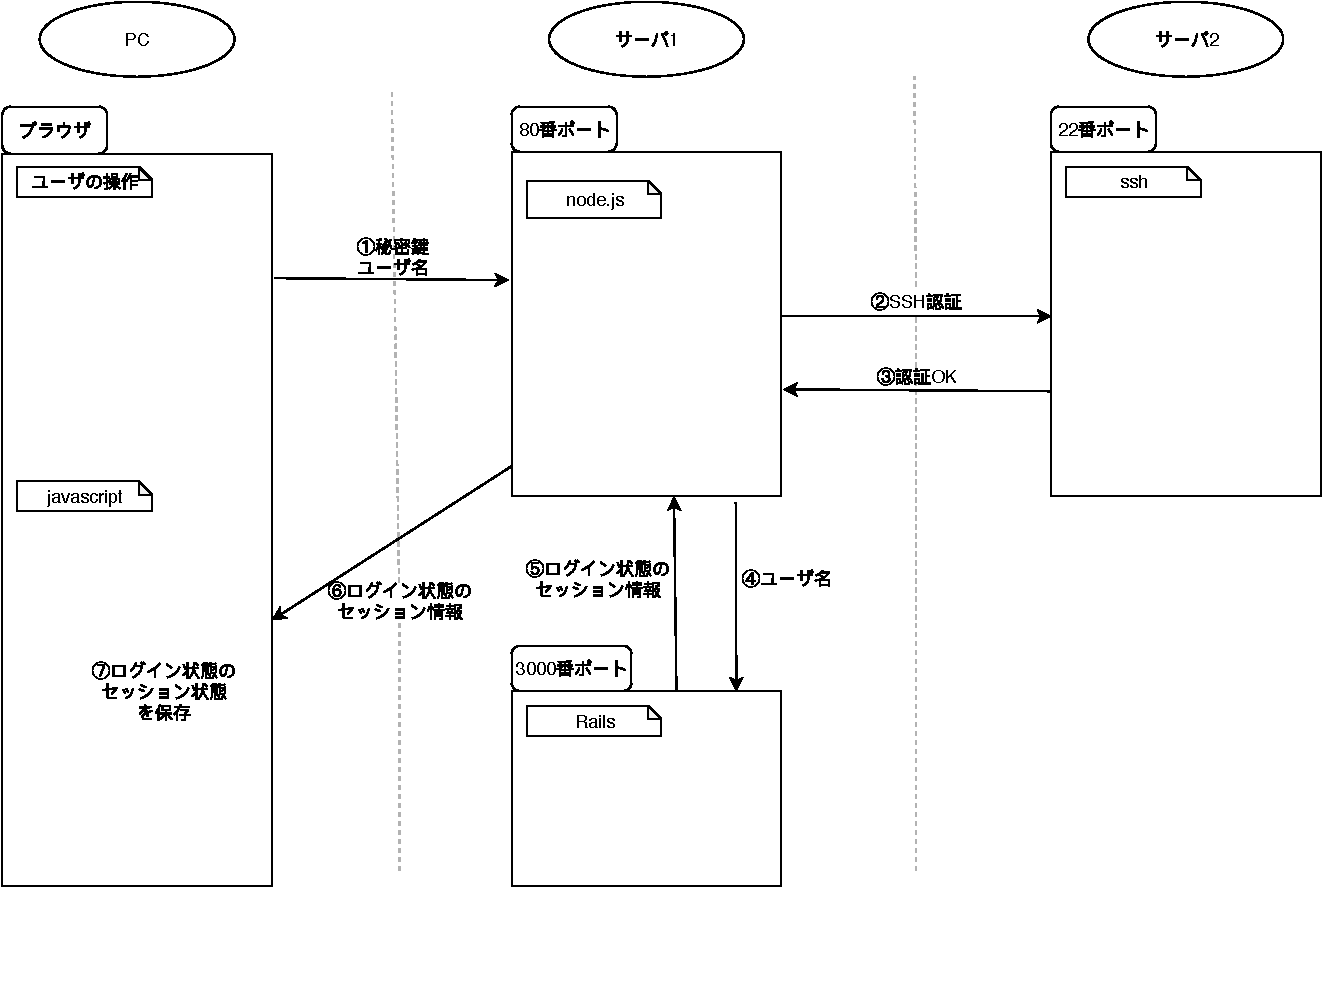
\includegraphics[width=13cm]{fig/chapter3/botu1-1.pdf}
    \caption{ログイン状態のセッション橋渡し案} 
    \label{botu1-1}
\end{figure}

%図を用いて(①とか)説明する
\noindent 図\ref{botu1-1}の\textcircled{\scriptsize 1} 〜 \textcircled{\scriptsize 3}では,エンドユーザはブラウザを用いて,公開鍵暗号方式によるsshをしている。
図\ref{botu1-1}の\textcircled{\scriptsize 4}では,HTTPリクエストのPOSTをしている。
図\ref{botu1-1}の\textcircled{\scriptsize 5}では,HTTPレスポンスが来て,そのヘッダ情報に「セッション情報をCookieに保存する」という情報が付与されている(のちのち,アクセス制限で,localhostからしかアクセスできないようにする).
図\ref{botu1-1}の\textcircled{\scriptsize 6}では,図\ref{botu1-1}の\textcircled{\scriptsize 5}の情報を,ブラウザのjavascript側にsocket通信で渡す.
最後に,図\ref{botu1-1}の\textcircled{\scriptsize 7}で,ログイン状態のセッション情報をCookieに保存する.
\\\\
\noindent ブラウザを用いての検証\\
ログイン中のセッション情報を,ブラウザのCookieに保存することで,ログインすることが可能かを検証する。\\
検証環境\\
 \quad 機器\\
  \qquad MacBook Pro (Retina, 13-inch, Early 2015)\\
  \qquad macOS High Sierra(バージョン10.13.6)\\
 \quad サーバ側\\
 \qquad Ruby on Rails(6.0.2.1)\\
 \qquad localhost:3000\\
 \quad ユーザ側\\
 \qquad 2っのブラウザ\\
 \qquad \quad Google Chrome\\
 \qquad \quad Google Chrome Canary\\
Cromeの開発環境(デベロッパーツール)を用いて以下の検証を行った。\\
まず,ログインした際の動きとして,HTTPレスポンスのヘッダ情報に,set-cookieがある.Cromeのデベロッパーツールでは,以下の図\ref{login-1}と表示される.\\
 \begin{figure}[h]
    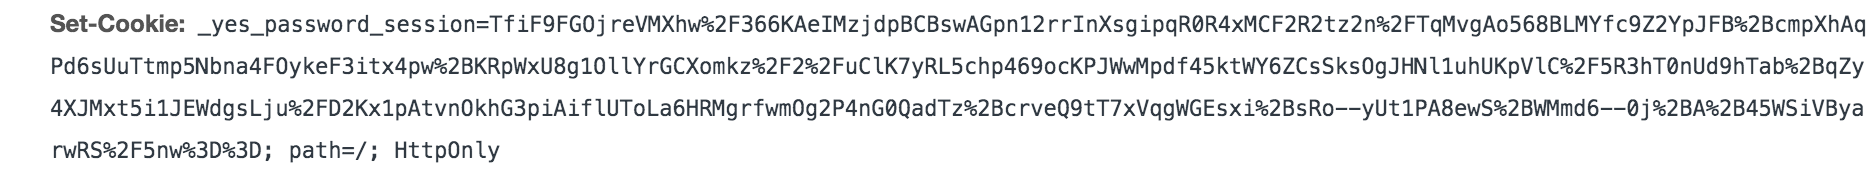
\includegraphics[width=13cm]{fig/chapter3/login-1.png}
    \caption{ログイン成功した際の,HTTPレスポンスの抜粋} 
    \label{login-1}
\end{figure}

\noindent 次に,図\ref{login-1}のHTTPレスポンスを元に,ブラウザのCookieにセッション情報を保存する。
Cromeのデベロッパーツールでは,以下の図\ref{login-2}と表示される.\\
\begin{figure}[h]
    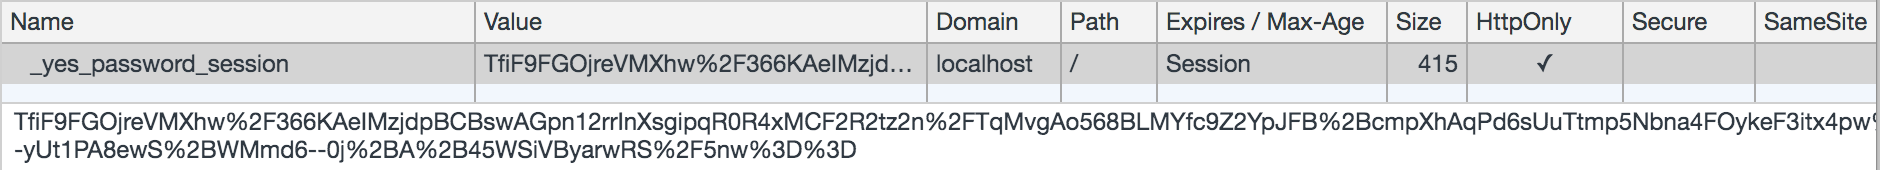
\includegraphics[width=13cm]{fig/chapter3/login-2.png}
    \caption{ブラウザのCookieのセッション情報}
    \label{login-2}
\end{figure}
上記の\ref{login-1},\ref{login-2}は,HTTPレスポンスのヘッダ情報で,ブラウザのCookieに値を保存している.その後,HTTPリクエストで,Cookie情報を付与\cite{cookie1}することにより,ステートレスなプロトコルであるHTTP上で,状態管理ができる\cite{cookie2}(ログイン状態の維持).
\\
現状で以下の図\ref{login_compare-1}のように,ログインしているブラウザ,ログインしていないブラウザがある.\\
\begin{figure}[h]
    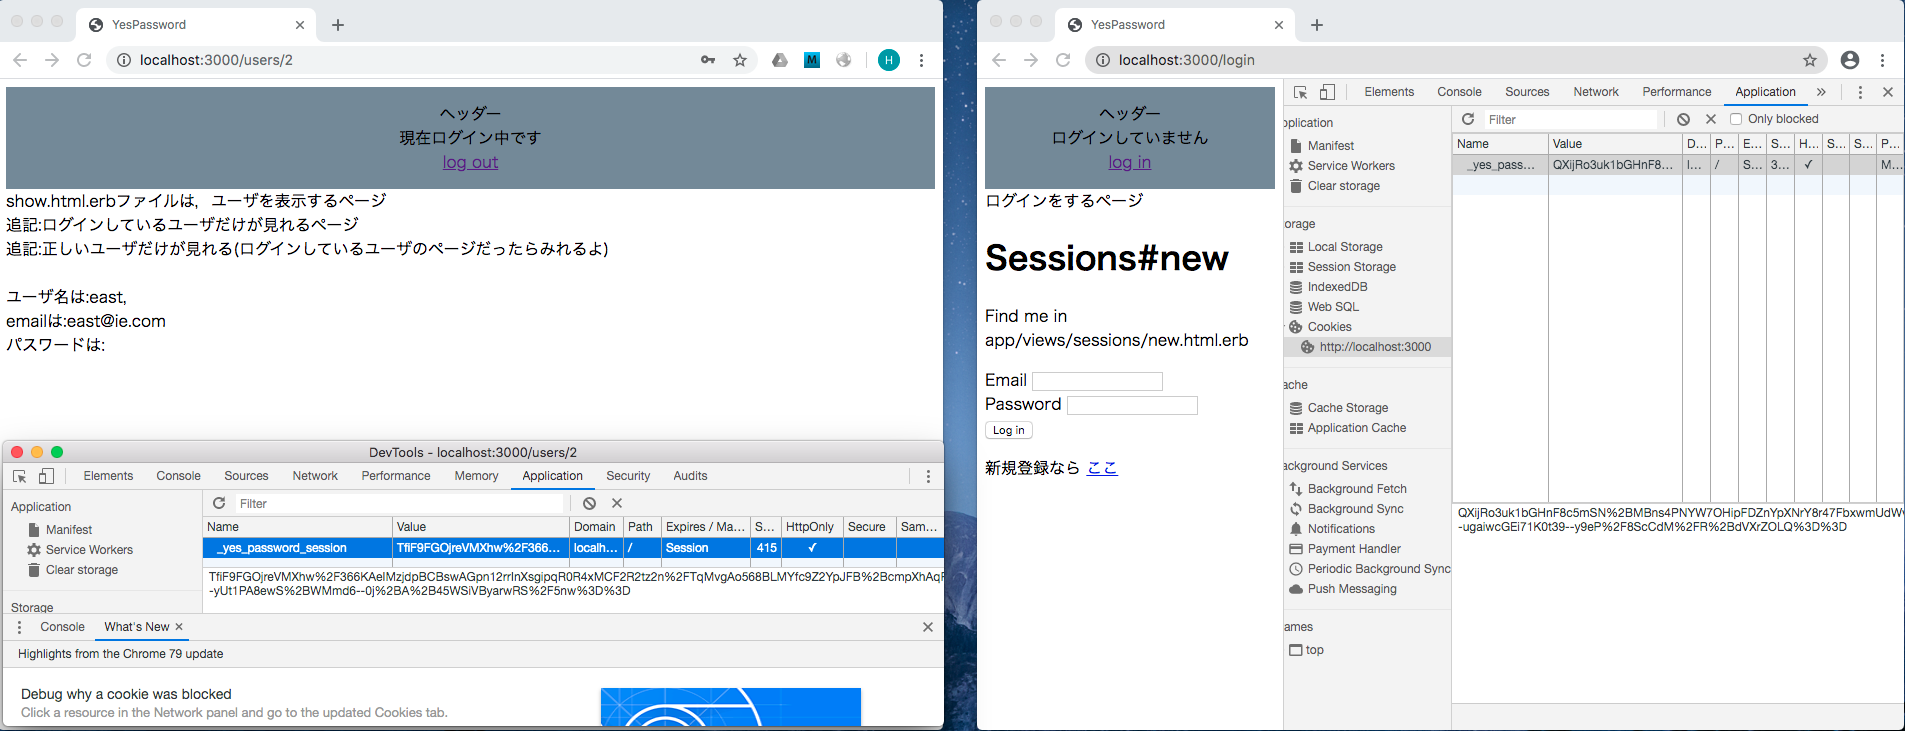
\includegraphics[width=13cm]{fig/chapter3/login_compare-1.png}
    \caption{2っのブラウザ(ログイン状態,ログインしていない状態)} 
    \label{login_compare-1}
\end{figure}
\\
上記の図\ref{login_compare-1}の状態から次の操作を行う.デベロッパーツールを用いて,ログインしているブラウザから,ログインしていないブラウザに,Cookie情報の,コピーアンドペーストを行い.リロードする.
その際の,状態が以下の図\ref{login_compare-2}になり,ログイン状態のセッションを橋渡し(Cookieに保存)することにより,ログインすることができることがわかる.\\
\begin{figure}[h]
    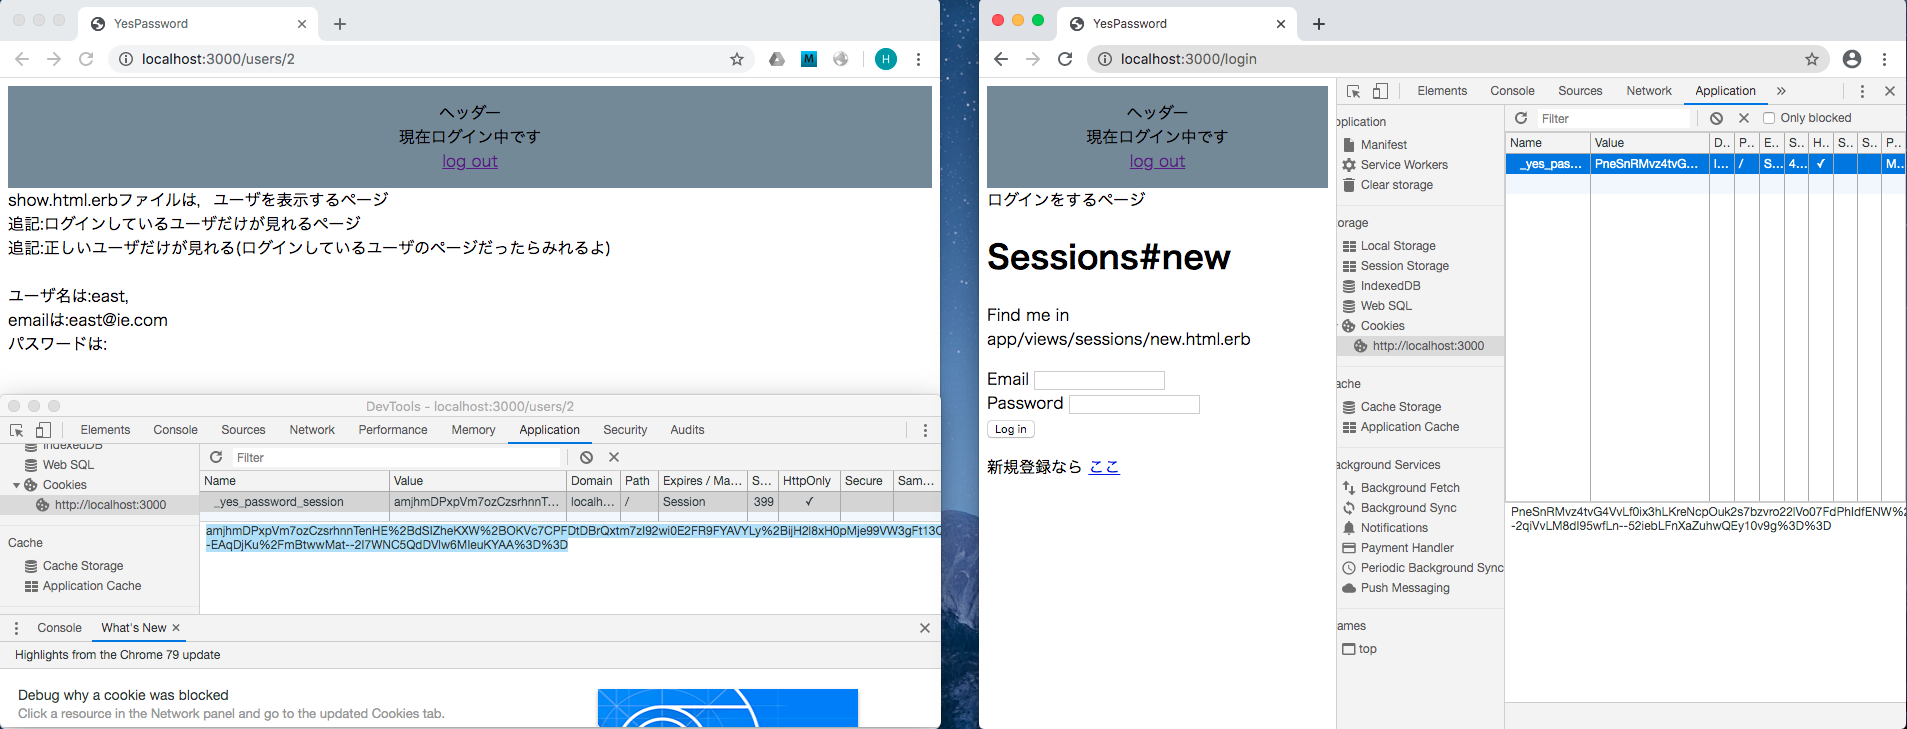
\includegraphics[width=13cm]{fig/chapter3/login_compare-2.png}
    \caption{2っのブラウザ(ログイン状態,ログイン状態)} 
    \label{login_compare-2}
\end{figure}
\\
図\ref{login_compare-2}の補足.\\
HTTPリクエストをする際に,新しいCookie情報が付与されることが確認できた.そのことにより,ログイン中の2っのブラウザが別のセッションになっている.
\\\\
\noindent 実際に実装\\
実際に実装を進めて,図\ref{botu1-1}の\textcircled{\scriptsize 1} 〜 \textcircled{\scriptsize 6}までできた.しかしながら,図\ref{botu1-1}の\textcircled{\scriptsize 7}ができなかった.その理由を以下の図\ref{botu1-2.pdf}を元に説明する.
\begin{figure}[h]
    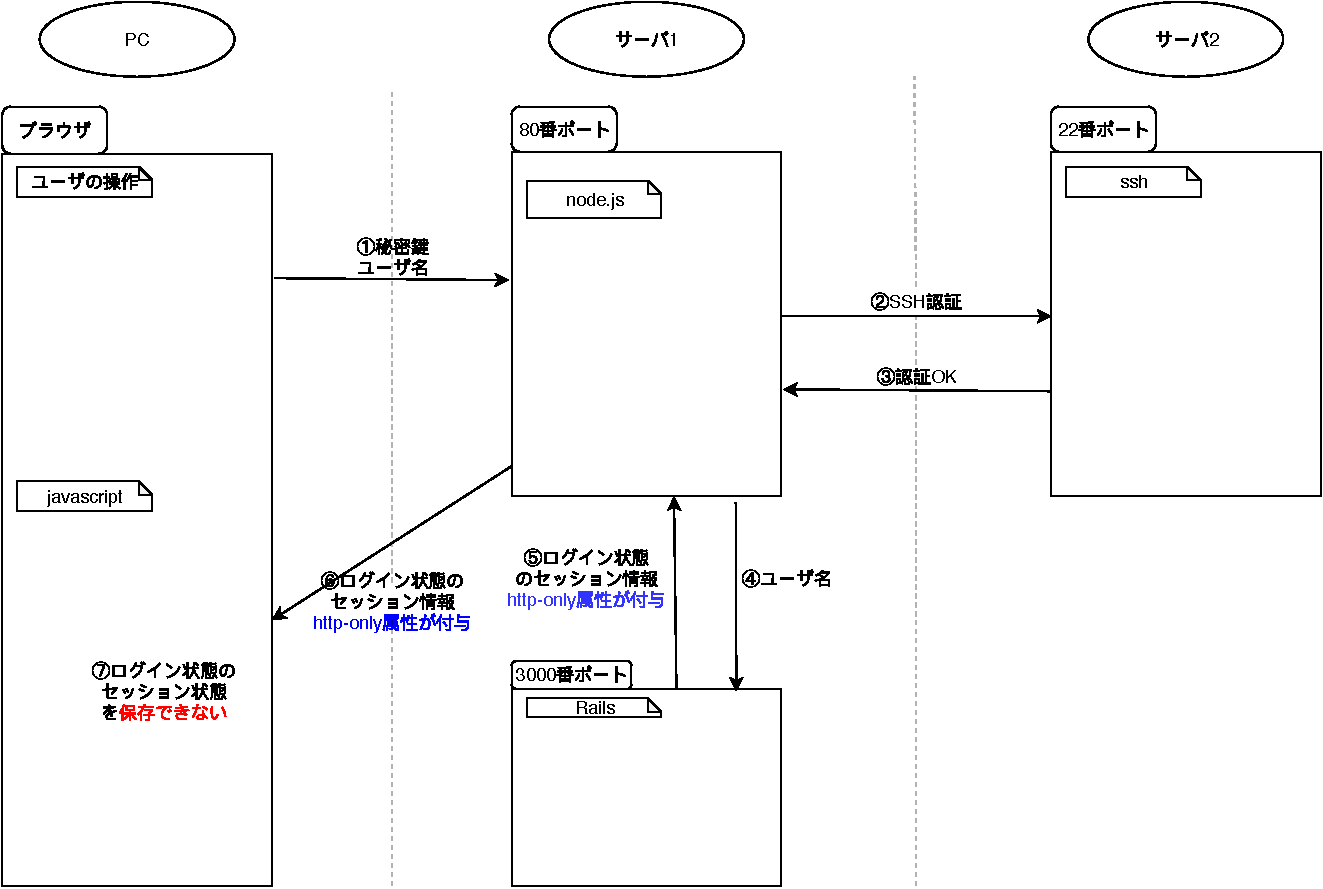
\includegraphics[width=13cm]{fig/chapter3/botu1-2.pdf}
    \caption{ログイン状態のセッション橋渡し案がボツになった} 
    \label{botu1-2.pdf}
\end{figure}
\\
図\ref{botu1-2.pdf}の\textcircled{\scriptsize 5} で,railsではセッションを発行する際に,http-only属性を付与している\cite{cookie-httponly-default}.そのことは,ログイン時のHTTPレスポンスである図\ref{login-1}でも現れている.
http-only属性がついたCookieは,javascriptで扱うことができなくなり,セッションハイジャックの対策を行っている\cite{cookie-httponly-security}.
そのため,図\ref{botu1-2.pdf}の\textcircled{\scriptsize 7}のように,セッション状態を保存することができなかったため,「ログイン状態のセッション橋渡し」の案はボツになった.
%
%
%図を用いながら,できない説明。
%  ( 図で,考案のどこまでできたかを示そうマル6までできたが,⑦でできなかった)
%そのためこの案はボツになった


% 実験
\chapter{検証}
\label{chap:poordirection}


\section{検証1}

\subsection{検証背景}

\subsubsection{検証目的}

password認証方式の,新規登録・認証の面倒さを解決するために,第3章の提案手法で
password認証方式に変わる,公開鍵暗号方式によるssh認証を用いた,WEBサービス認証の提案を行った。\\
しかしながら,提案だけだと,新規登録・認証の面倒さを解決していることの根拠に乏しい。
よって,検証を行い,第3章の提案手法は"面倒さの軽減"に効果的に繋がっているかの確認をする。


\subsubsection{検証手段}

検証の手段としては,実際に,以下の2つの認証方式の登録・認証を被験者に体験してもらう。
%また,実験マニュアルを作成し,実験者は被験者に対して,同じように接するようにする。

\begin{itemize}
  \item バグあり,パスワード方式認証(以後 "パスワード認証"と記述する)
  \item 公開鍵暗号暗号方式によるssh認証(以後 "鍵認証”と記述する)
\end{itemize}

※バグは「認証の際に,どんなパスワードでも認証してしまう」\\
その後,2つの観点から,"面倒さ"を数値化する。
1つ目の観点は「時間」である。
"面倒さ"をアカウント登録・認証にかかる時間と推測し,計測化する。
詳しい詳細については,検証環境のマニュアルに記述する。
%まず,パスワード 形式による登録・認証の時間計測をそれぞれ行う。
% 次に,公開鍵暗号方式によるSSH 形式登録・認証の時間計測をそれぞれ行う。
% 最後に,上記の形式による時間計測を比較する。
2つ目の観点は「アンケート」である。
アンケートには,点数で答える方式,文字で記入する欄 の2つがあり,点数で答える方式により"面倒さ”を数値化する。
アンケートの細かい内容は,4.1.3の検証画面に記述する。

また,アンケートには"面倒さ"を数値化する以外にも,以下の2つの意味を込める。
1つ目の意味は次の通りである。
アカウント登録・認証にかかる時間 を,"面倒さ"と予想して検証しているが,その予想を確かめる必要がある。
アンケートを取ることにより,「アカウント登録・認証にかかる時間」と,「アンケートによる面倒さ」が比例していることを確認することで,予想を確かめることができる。
また,被験者の状態も確認することで,面倒と感じるのが,検証自体に対しての面倒さと関係があるのかを確認する。
2つ目の意味は次のとおりである。
記入欄で,改善点や感じたことの意見をもらうことで,今後の研究に生きるようなアンケートをもらう。








\subsection{検証環境}
 \subsubsection{検証場所}
 第3章で記述したとおり,検証場所は学科のVMを用いているため,学科のネットワーク内(有線LAN,wifiアクセスポイント{ie-ryukyu})
 から,アクセスして検証を行う。


 %\subsubsection{検証画面}

 \subsubsection{検証の流れ}
    ここでは,被験者に行ってもらう,検証の流れを記述する。
    時間の観点で"面倒さ"を数値化する検証では,被験者にはパスワード方式,鍵方式の登録・認証をそれぞれ行ってもらう。その時,被験者は時間を測る。 
    また,再現性を持って,検証を行うためにマニュアルを作成し,マニュアル通りに検証を行う。
    アンケートの観点で"面倒さ"を数値化する検証では,
    時間の観点で"面倒さ"を数値化する検証 が終わった直後に行うようにすることで,被験者の思った感情とアンケート結果の差異が少なくなるようにする。
  

  \subsubsection{検証画面}
    %実際に記述--------------------------------------------------------
    ここでは,被験者に行ったもらう検証画面をのせる。

    以下の
    図\ref{検証1アカウント作成(パスワード方式)},
    図\ref{検証1認証(パスワード方式)}
    図\ref{検証1認証成功後(パスワード方式)}
    は,第3章の提案手法で実現したパスワード方式,登録・認証を,実際に被験者に行ってもらった時のブラウザ画面である。
    図\ref{検証1アカウント作成(パスワード方式)}は,アカウント登録画面である。
    図\ref{検証1認証(パスワード方式)}は,図\ref{検証1アカウント作成(パスワード方式)}で登録したアカウントに認証するための画面である。
    図\ref{検証1認証成功後(パスワード方式)}は,図\ref{検証1認証(パスワード方式)}で認証成功した後の画面である。
    % パスワード方式のスクショ---------------------------
    \vspace{4cm}%図の位置を正しくする!
    %\begin{figure}[h]
    \begin{figure}[H]
        %\centering
        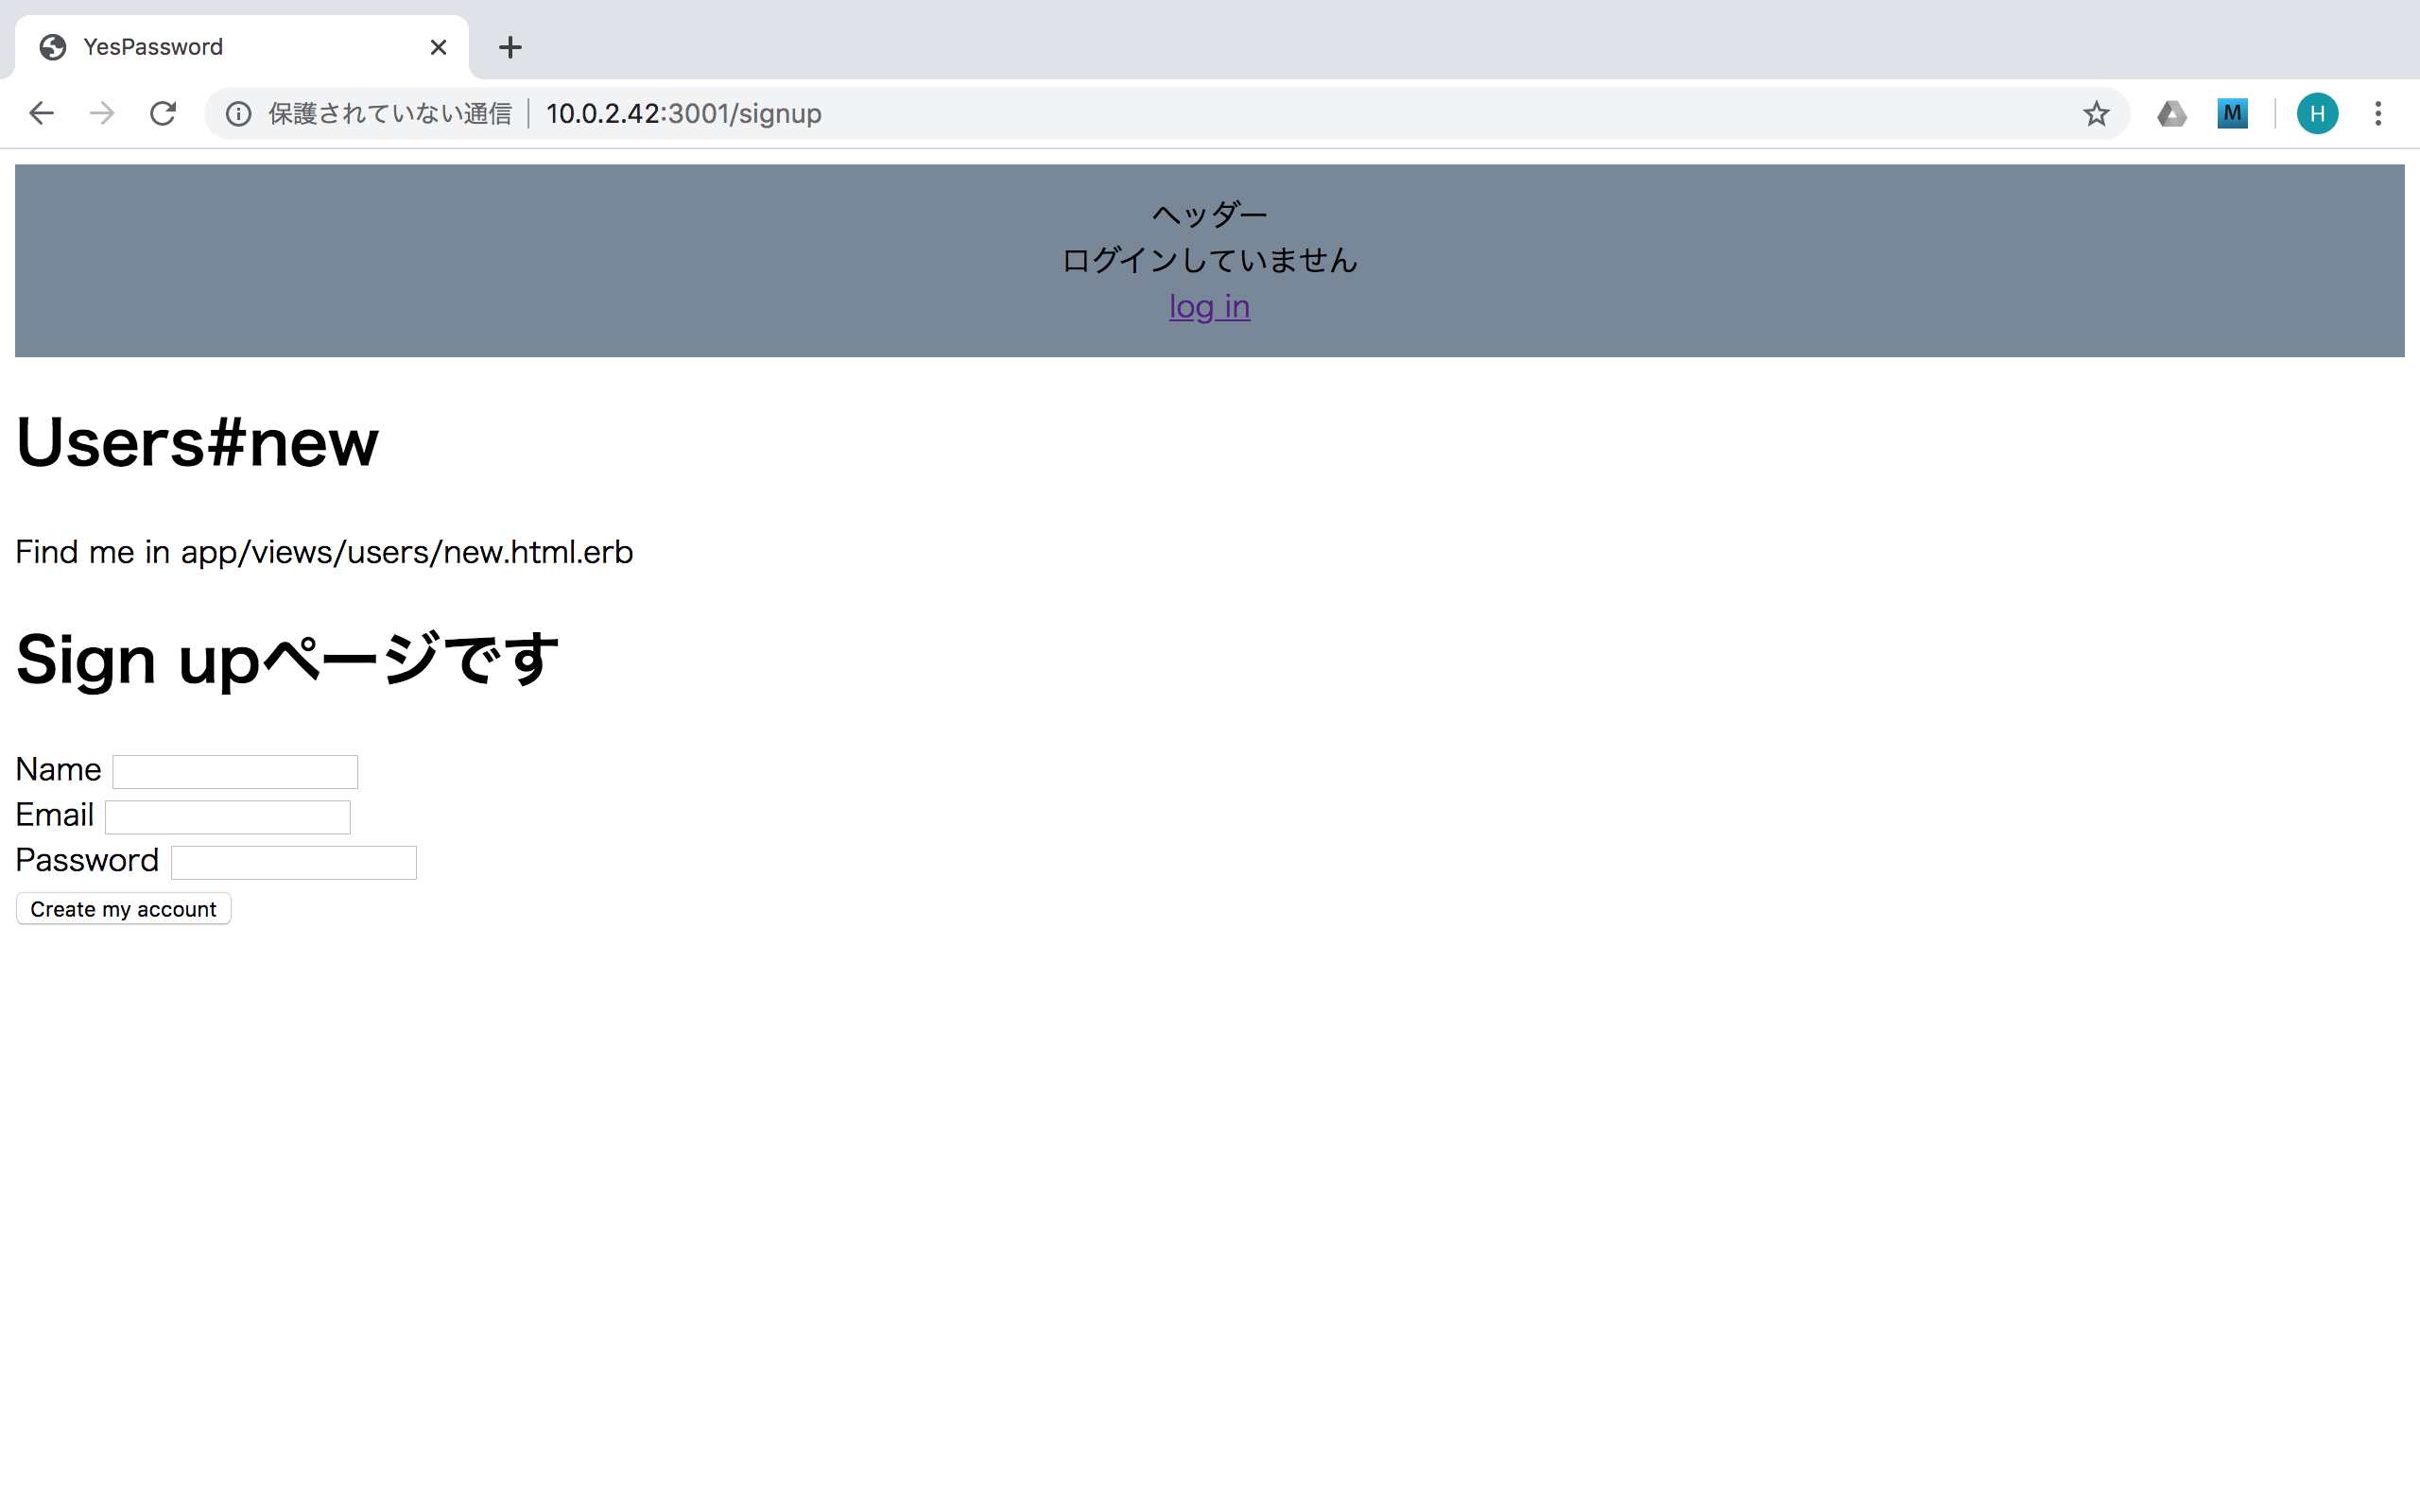
\includegraphics[height=8.4cm]{./fig/chapter4/inspect_1/password_screnn/sign_up.png}
        \caption{検証1\_アカウント作成(パスワード方式)}
        \label{検証1アカウント作成(パスワード方式)}
    \end{figure}

    \vspace{4cm}%図の位置を正しくする!
    \begin{figure}[H]
        %\centering
        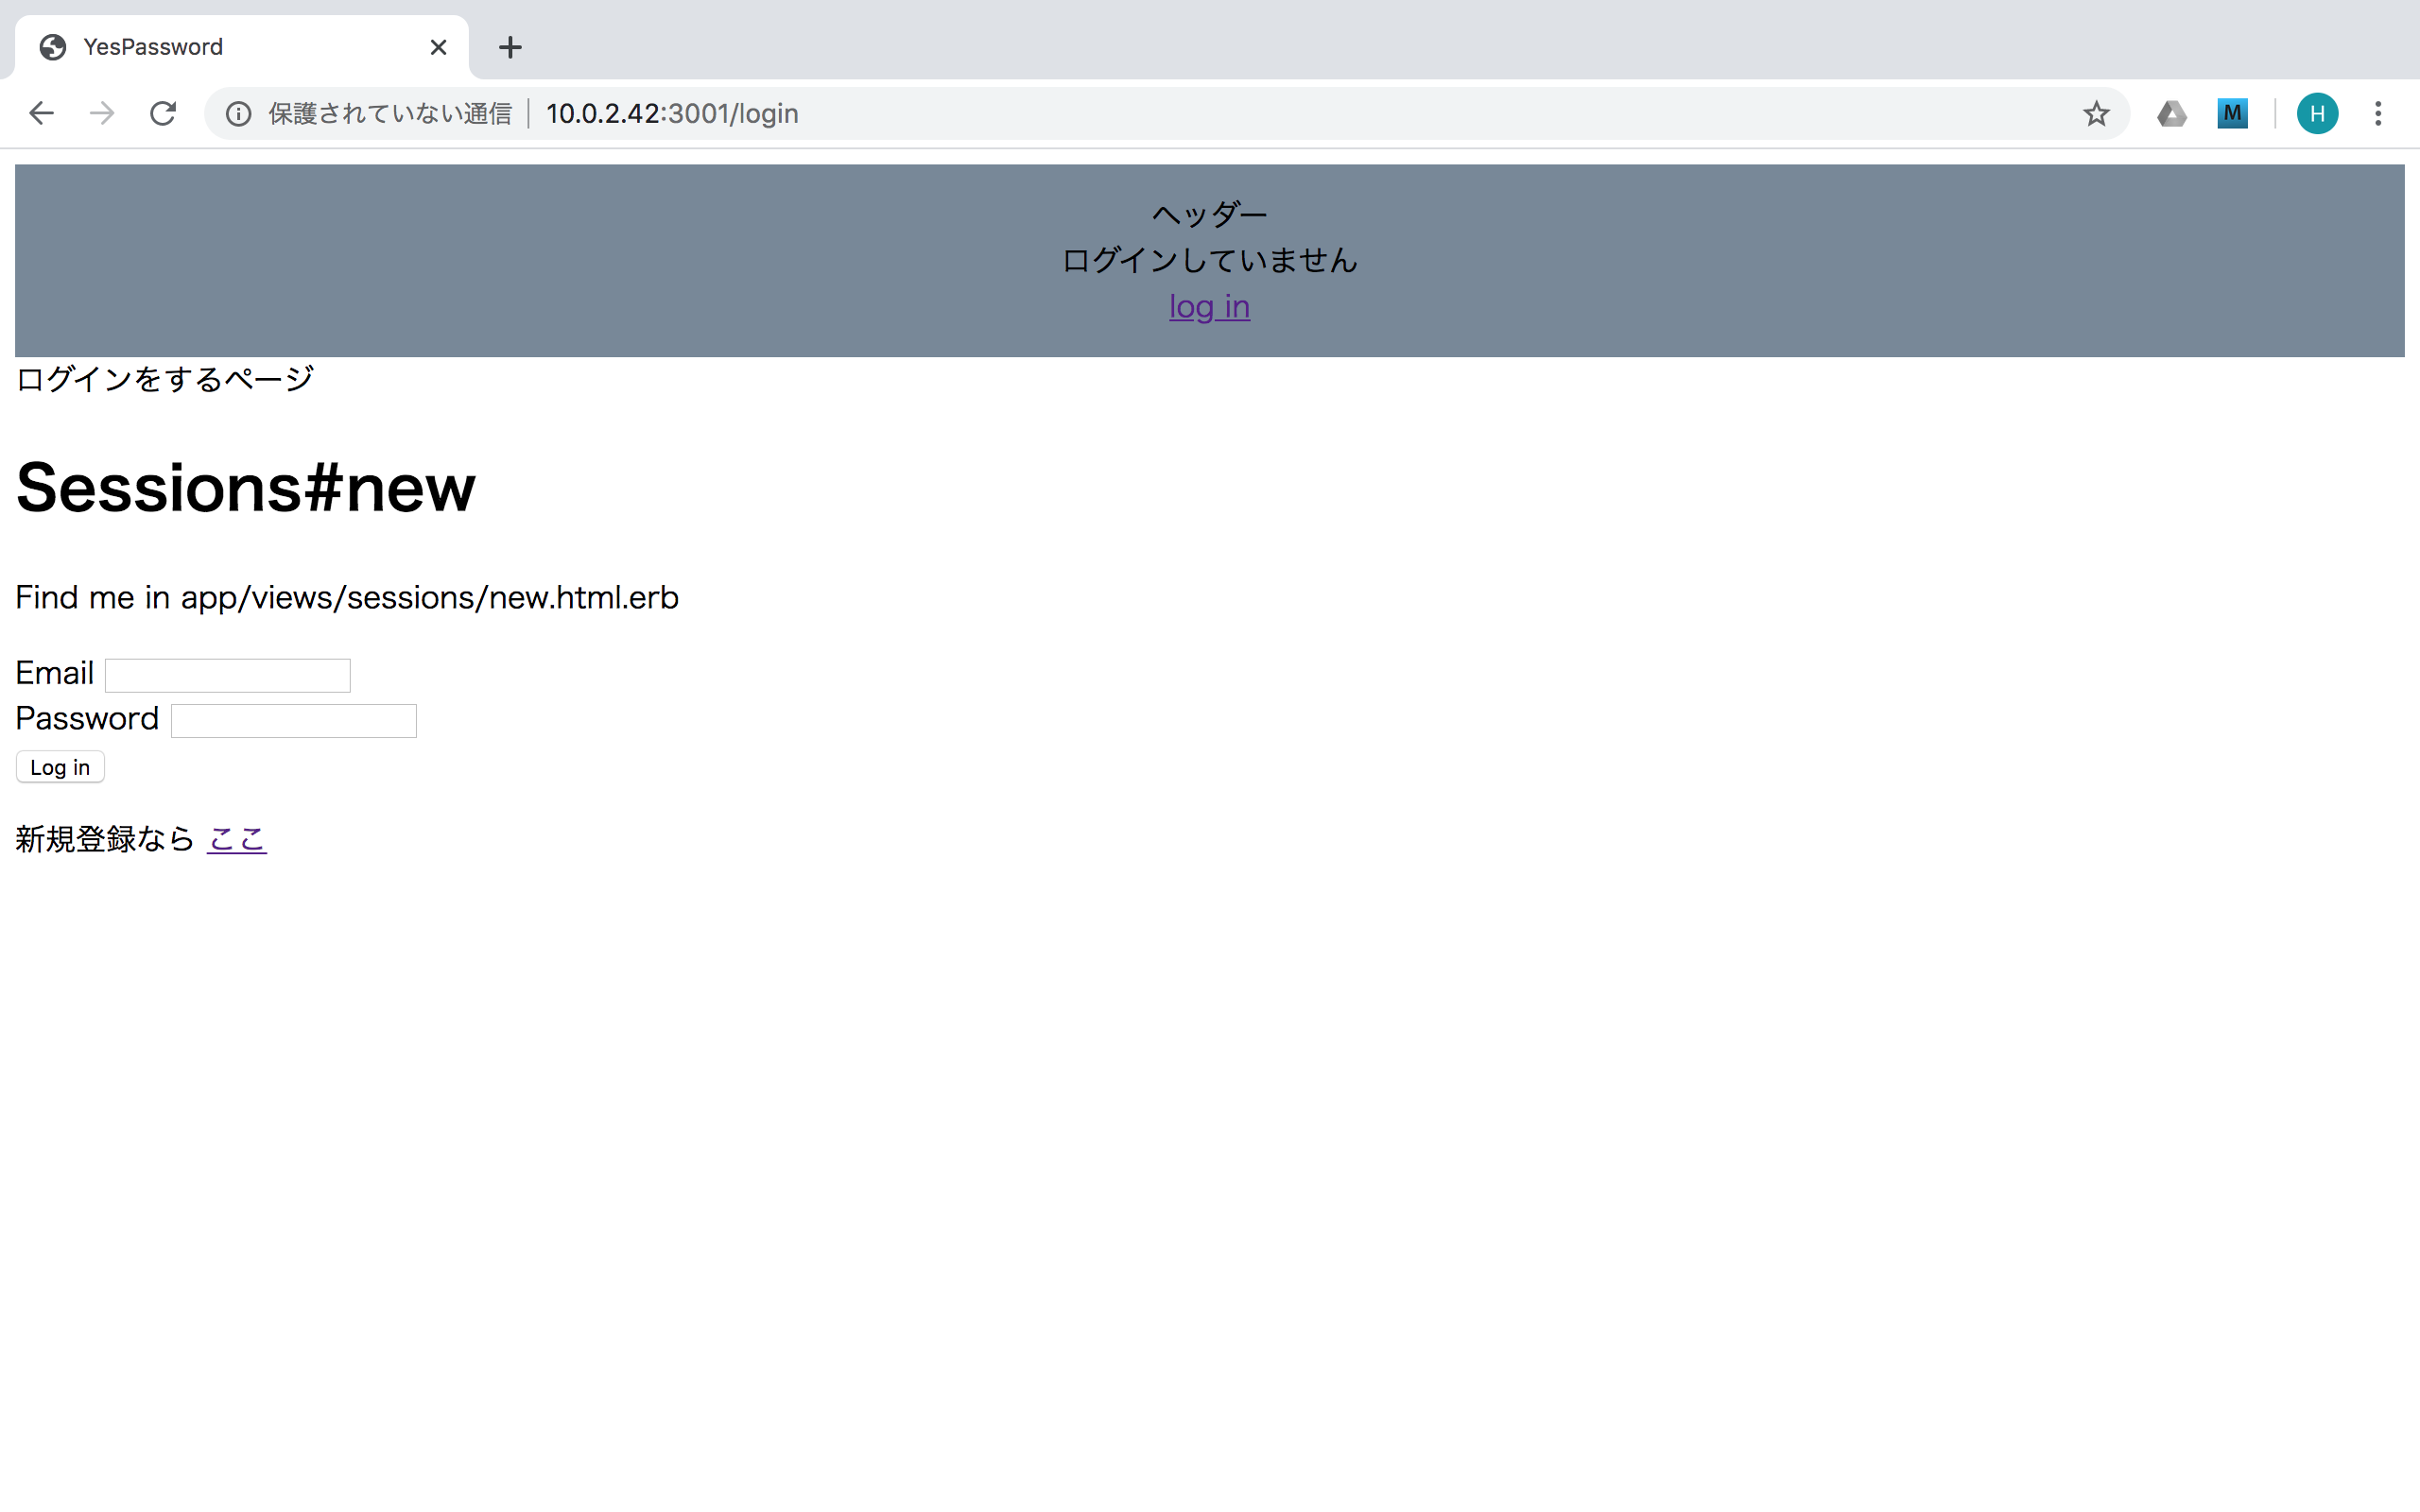
\includegraphics[height=8.4cm]{./fig/chapter4/inspect_1/password_screnn/login.png}
        \caption{検証1\_認証(パスワード方式)}
        \label{検証1認証(パスワード方式)}
    \end{figure}

    \vspace{4cm}%図の位置を正しくする!
    \begin{figure}[H]
        %\centering
        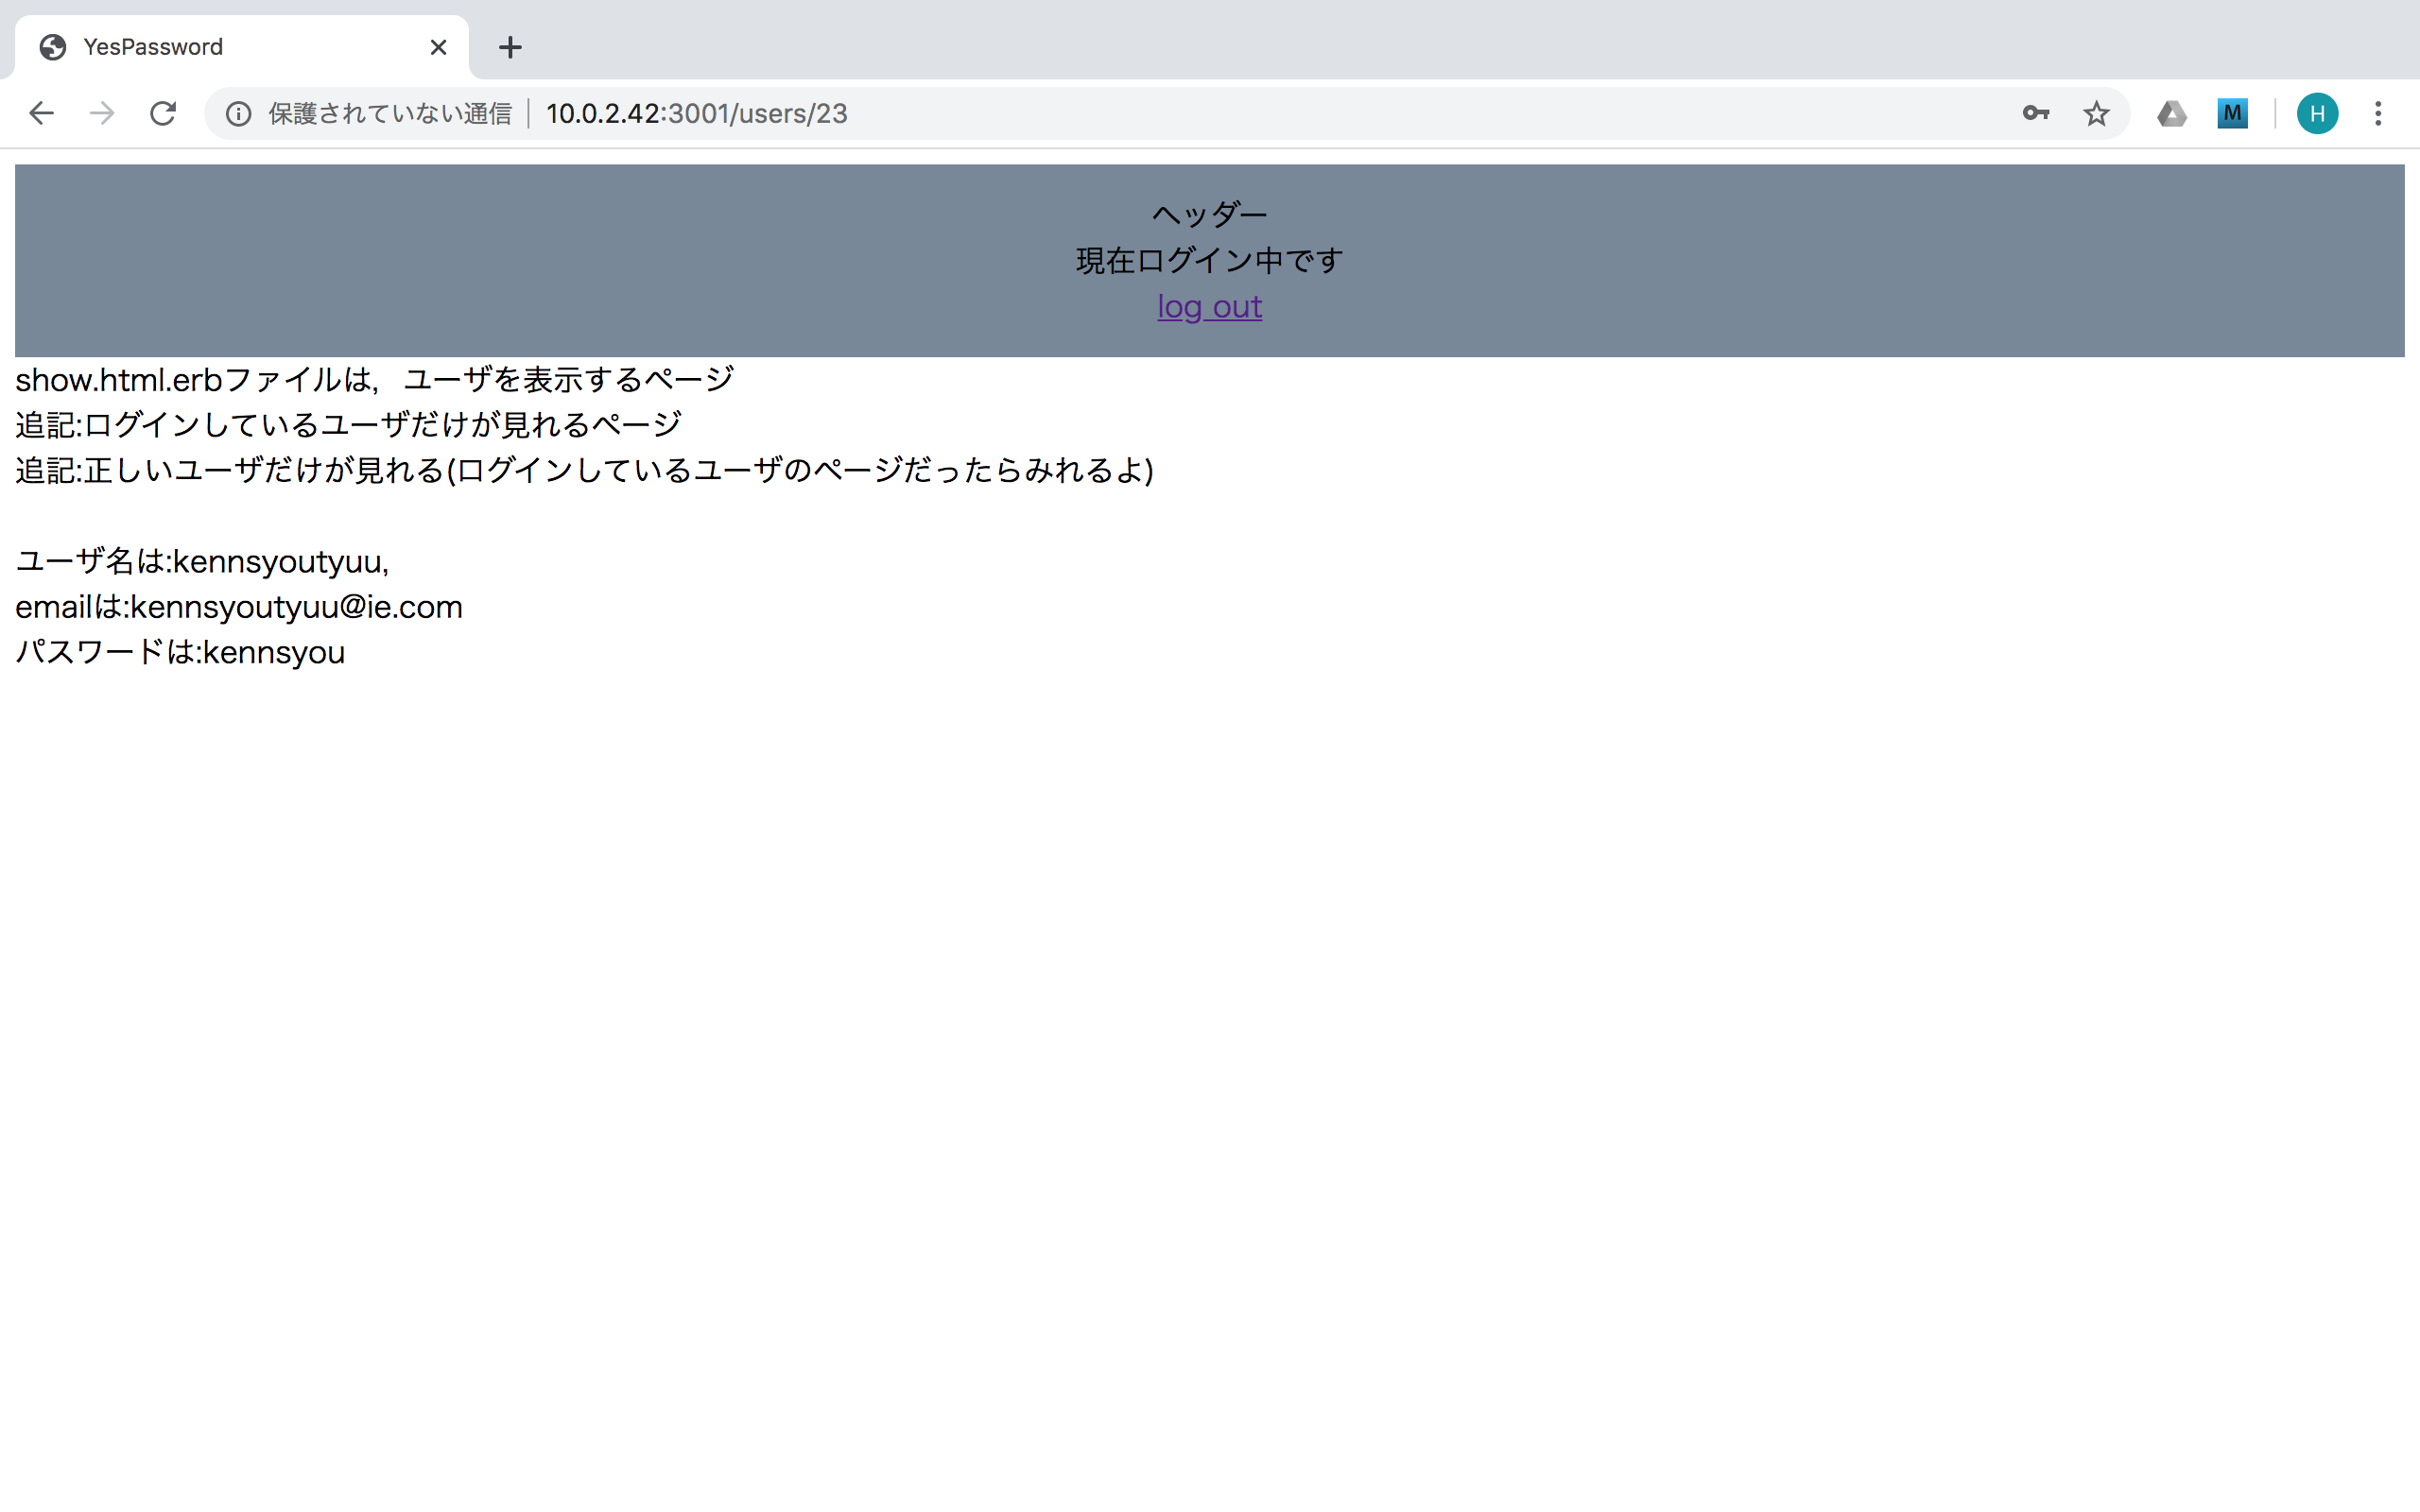
\includegraphics[height=8.4cm]{./fig/chapter4/inspect_1/password_screnn/success.png}
        \caption{検証1\_認証成功後(パスワード方式)}
        \label{検証1認証成功後(パスワード方式)}
    \end{figure}
    % パスワード方式のスクショ---------------------------








    \newpage
    \newpage

    以下の
    図\ref{検証1アカウント作成(鍵方式)},
    図\ref{検証1認証(鍵方式)}
    図\ref{検証1認証成功後(鍵方式)}
    は,第3章の提案手法で実現した,鍵方式の登録・認証を,実際に被験者に行ってもらった時のブラウザ画面である。
    図\ref{検証1アカウント作成(鍵方式)}は,アカウント登録画面である。
    図\ref{検証1認証(鍵方式)}は,図\ref{検証1アカウント作成(鍵方式)}で登録したアカウントに認証するための画面である。
    図\ref{検証1認証成功後(鍵方式)}は,図\ref{検証1認証(鍵方式)}で認証成功した後の画面である。
    % 鍵方式のスクショ----------------------------------
    \vspace{4cm}%図の位置を正しくする!
    \begin{figure}[H]
        %\centering
        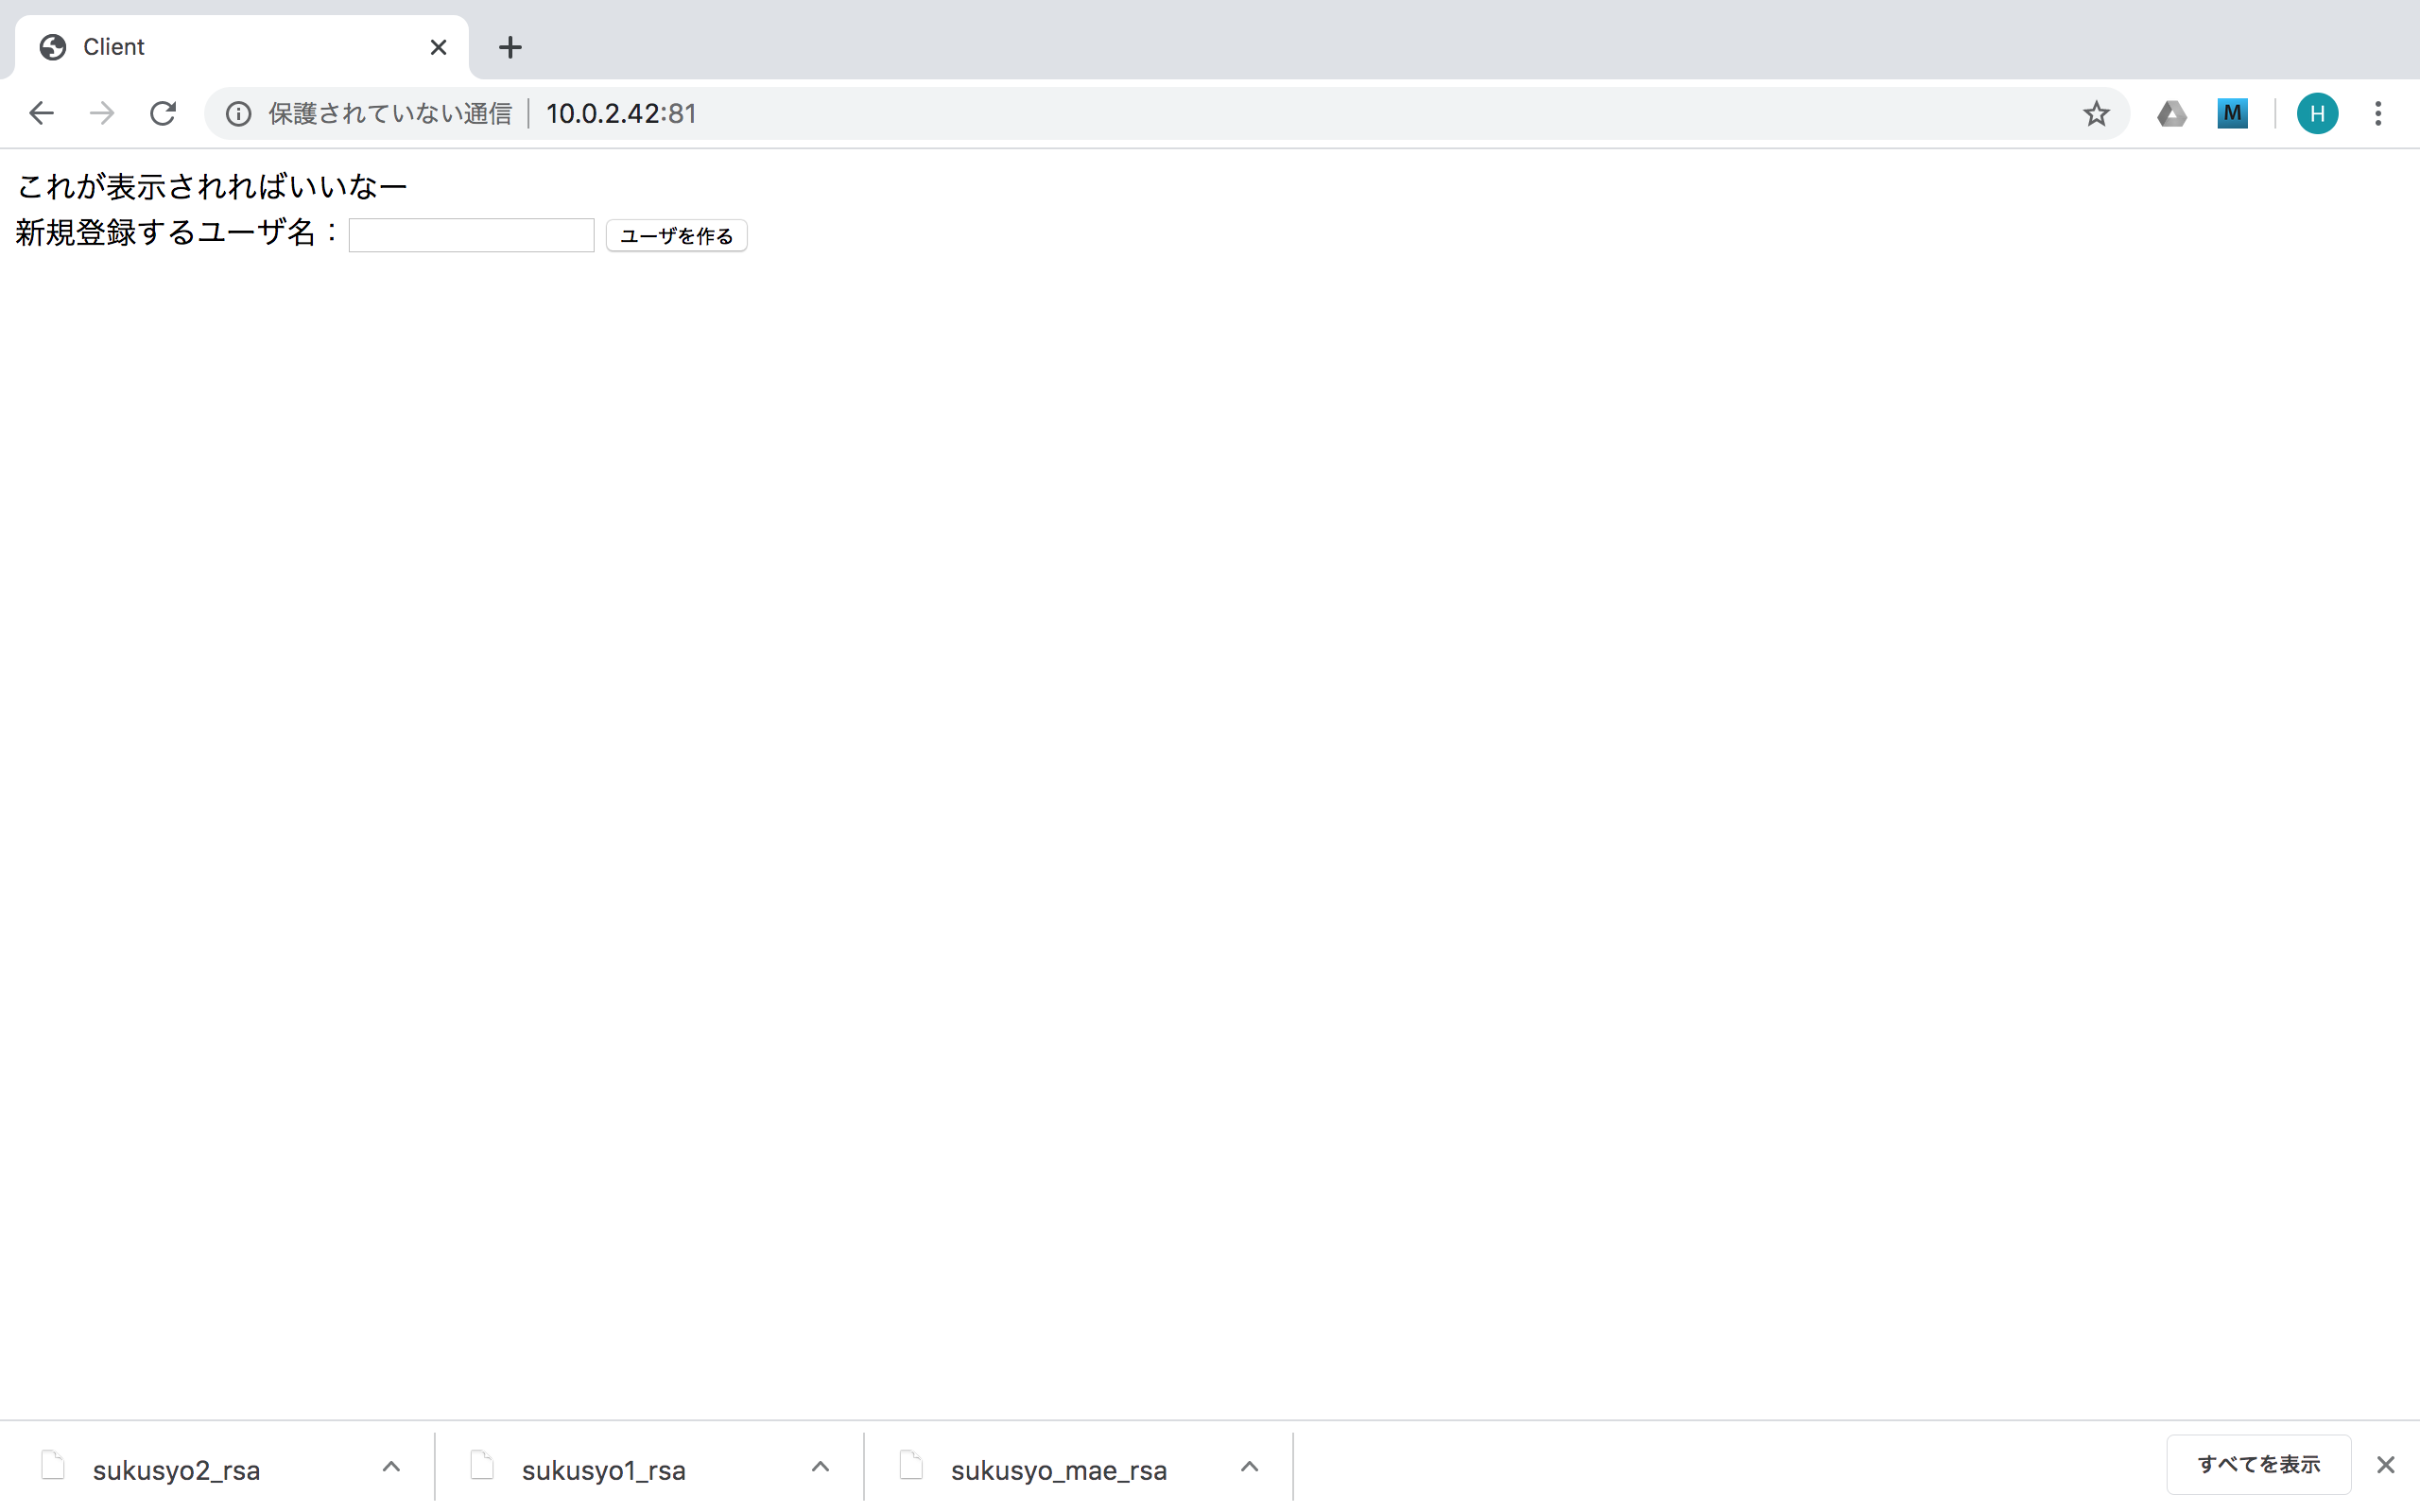
\includegraphics[height=8.4cm]{./fig/chapter4/inspect_1/key_screnn/sign_up.png}
        \caption{検証1\_アカウント作成(鍵方式)}
        \label{検証1アカウント作成(鍵方式)}
    \end{figure}

    \vspace{4cm}%図の位置を正しくする!
    \begin{figure}[H]
        %\centering
        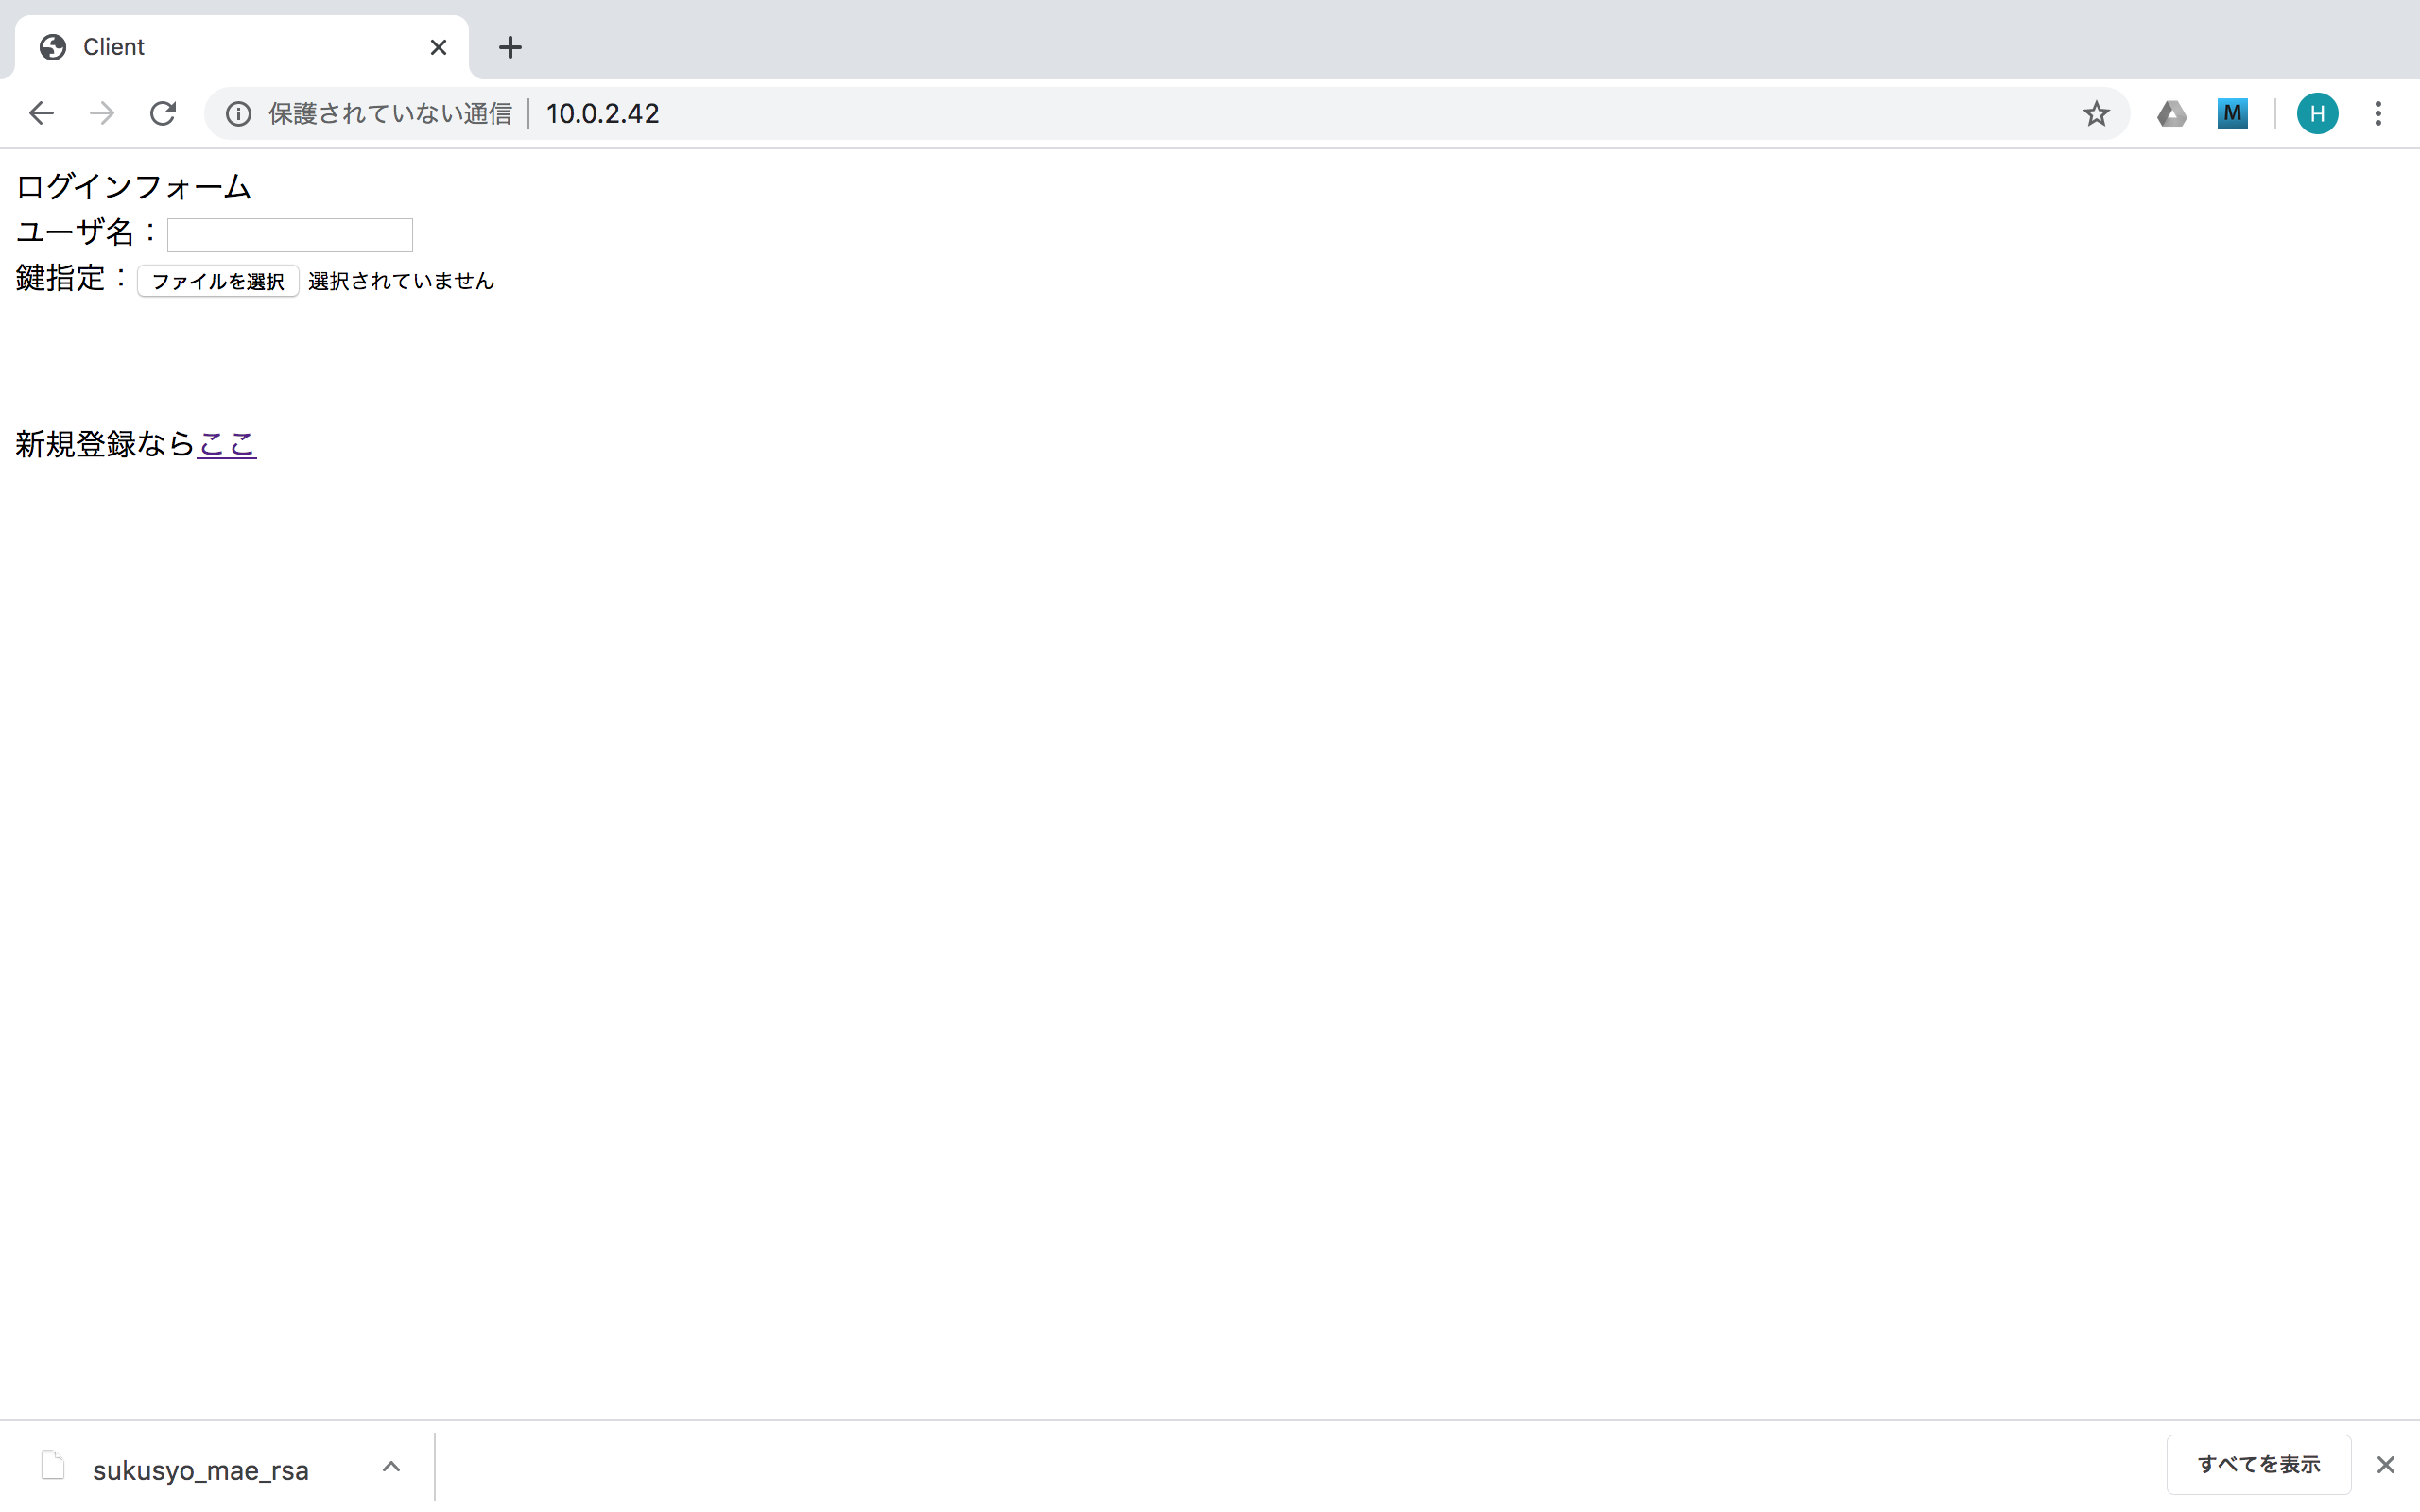
\includegraphics[height=8.4cm]{./fig/chapter4/inspect_1/key_screnn/login.png}
        \caption{検証1\_認証(鍵方式)}
        \label{検証1認証(鍵方式)}
    \end{figure}

    \vspace{4cm}%図の位置を正しくする!
    \begin{figure}[H]
        %\centering
        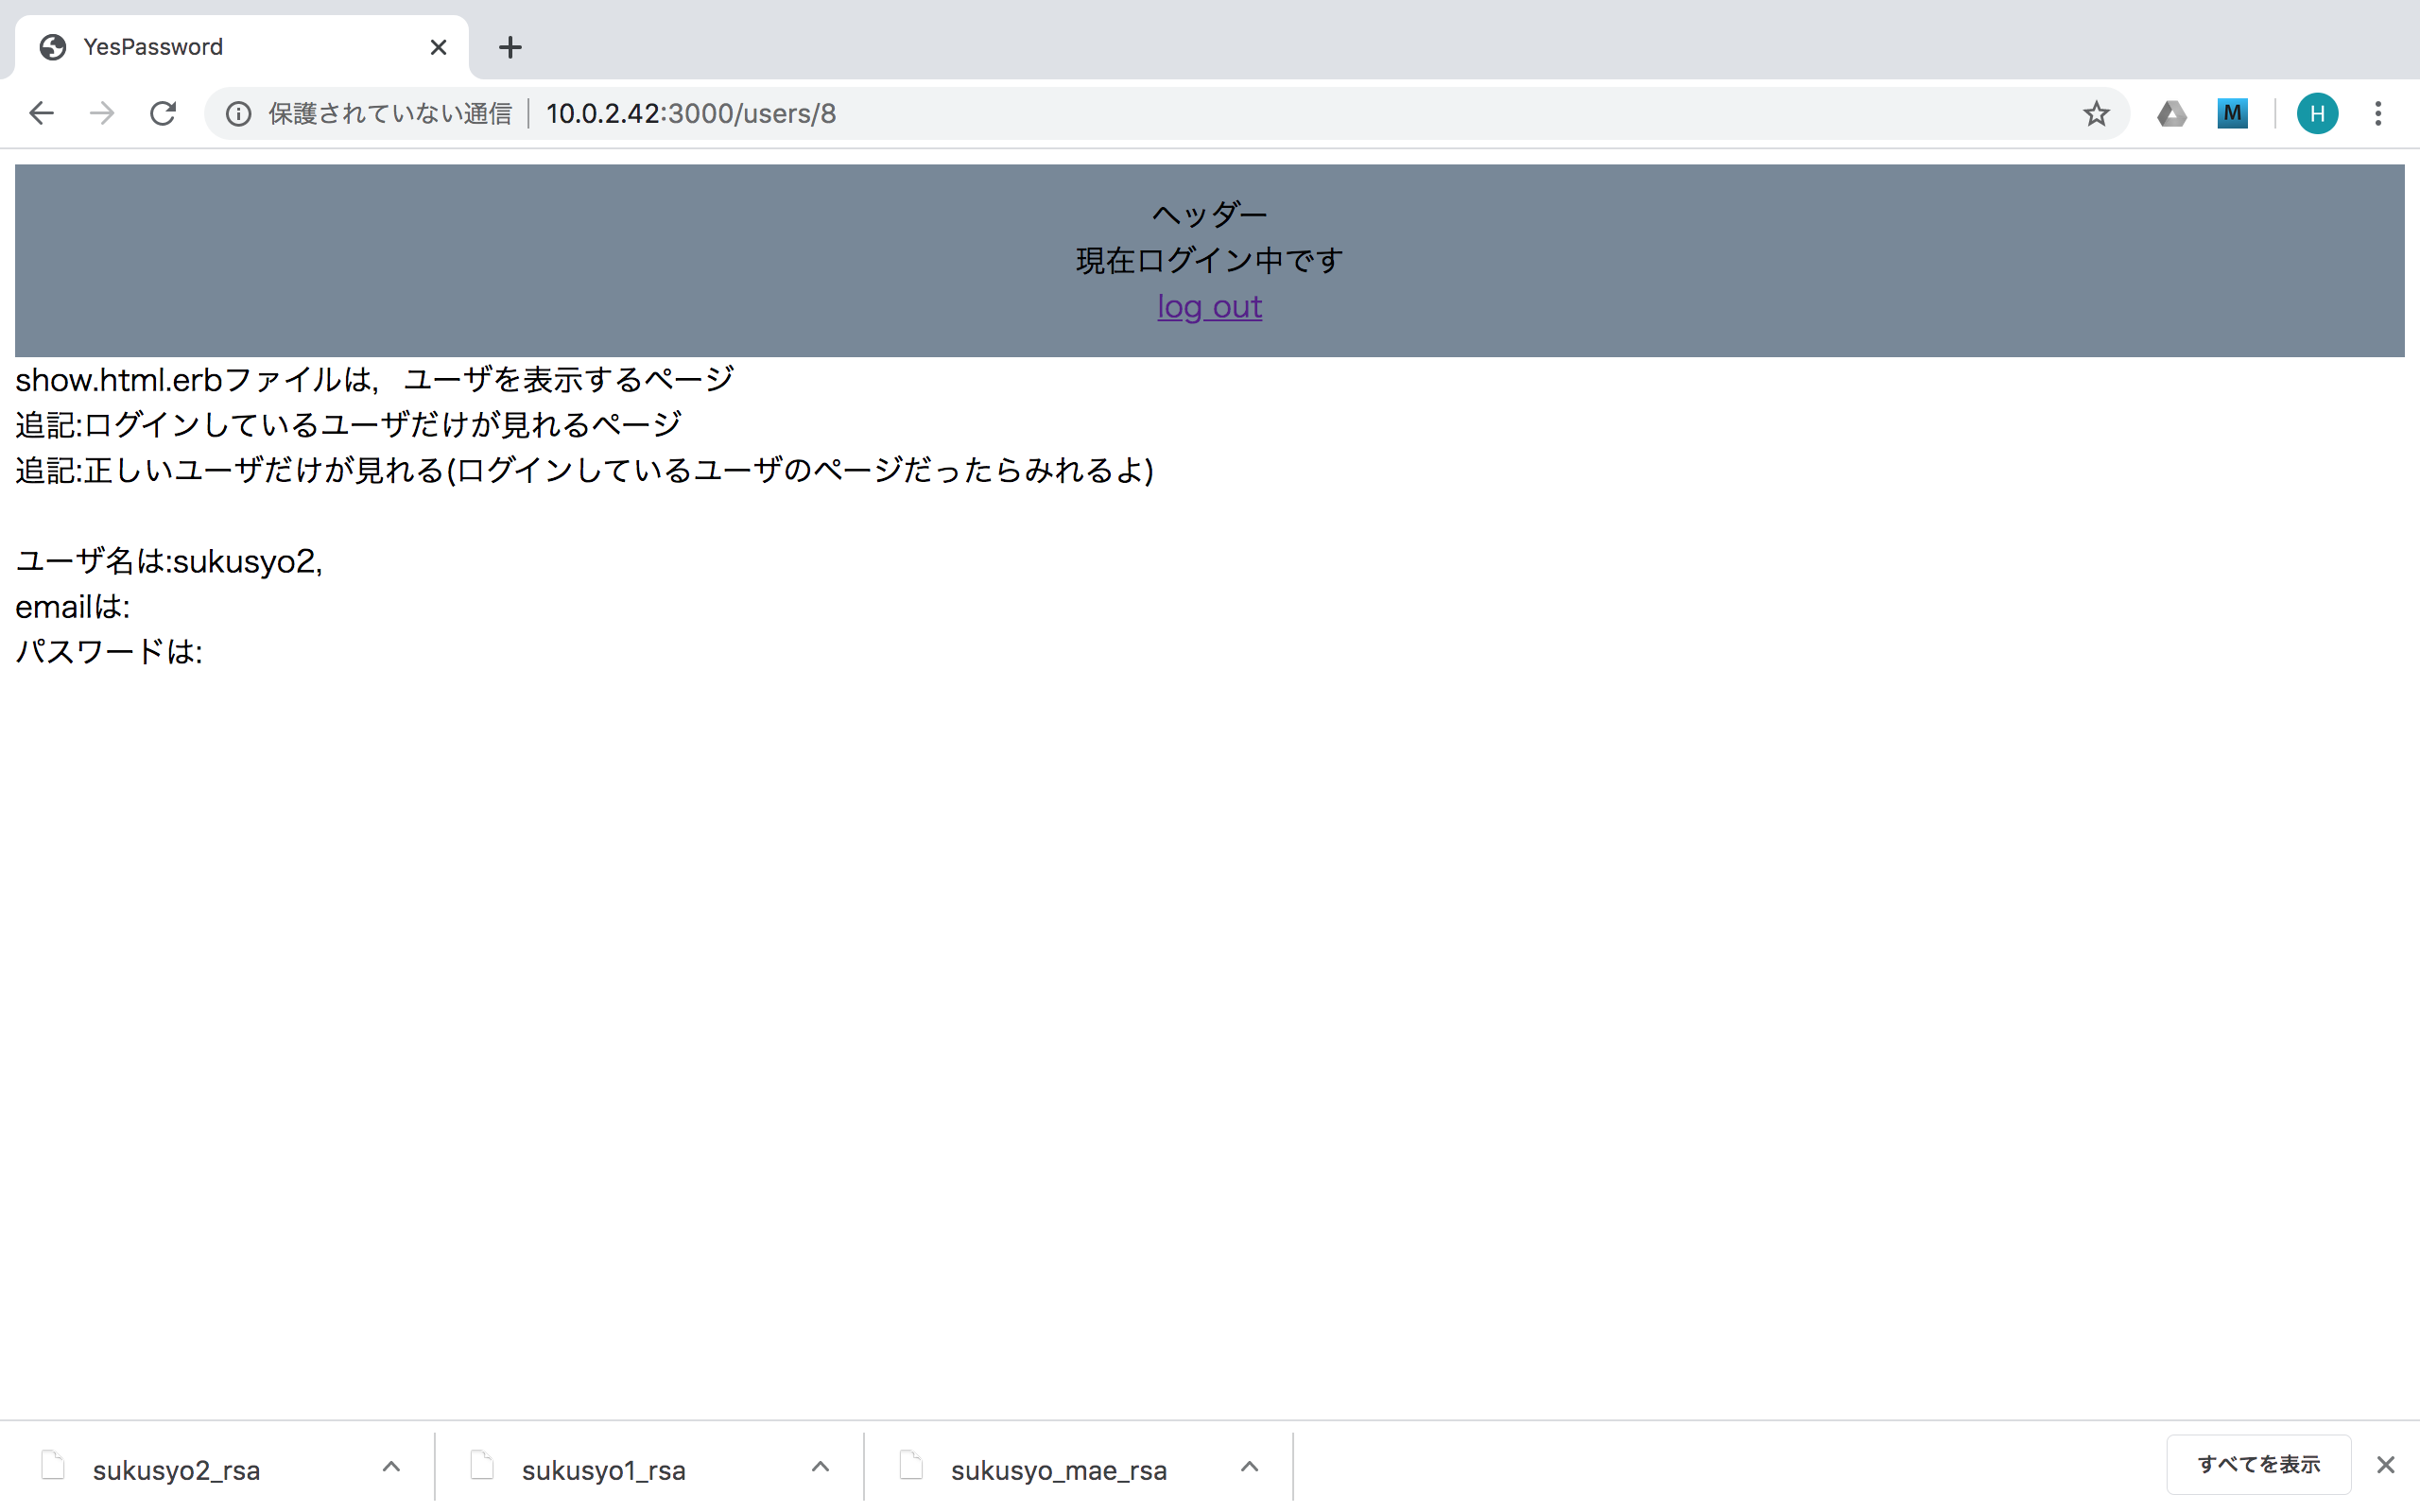
\includegraphics[height=8.4cm]{./fig/chapter4/inspect_1/key_screnn/login-after2.png}
        \caption{検証1\_認証成功後(鍵方式)}
        \label{検証1認証成功後(鍵方式)}
    \end{figure}
    % 鍵方式のスクショ----------------------------------





    

    以下の
    図\ref{アンケート1},
    図\ref{アンケート2},
    図\ref{アンケート3},
    図\ref{アンケート4}
    は
    図\ref{検証1アカウント作成(パスワード方式)} 〜 図\ref{検証1認証成功後(鍵方式)} までの,
    時間計測が終わった直後に行う,アンケートの画面である。
    %% アンケートの意図を説明
    % 検証自体面倒か
    図\ref{アンケート1} では,"検証自体の面倒さ"をアンケートで聞いている。
    その意図として,"面倒"と感じた感情は,検証役になること自体が面倒だったことに起因していないかを確かめるためである。
    % 登録・認証に対して,面倒と感じた度合いを
    図\ref{アンケート2}では,パスワード方式の登録・認証それぞれについて,どのくらい面倒かを質問している。
    図\ref{アンケート3}では,鍵方式の登録・認証それぞれについて,どのくらい面倒かを質問している。
    図\ref{アンケート2},図\ref{アンケート3}の質問の意図としては,アンケートの観点から"面倒さ"を数値化することである。
    図\ref{アンケート4}では,鍵方式の登録・認証について,被験者の技術視点と利用視点から,自由形式で意見を求めている。
    図\ref{アンケート4}の意図としては,よりよい物を作るために,被験者意見を収集し,今後の方針を決めるためである。

    % アンケートのスクショ----------------------------------
    \vspace{4cm}%図の位置を正しくする!
    \begin{figure}[H]
        %\centering
        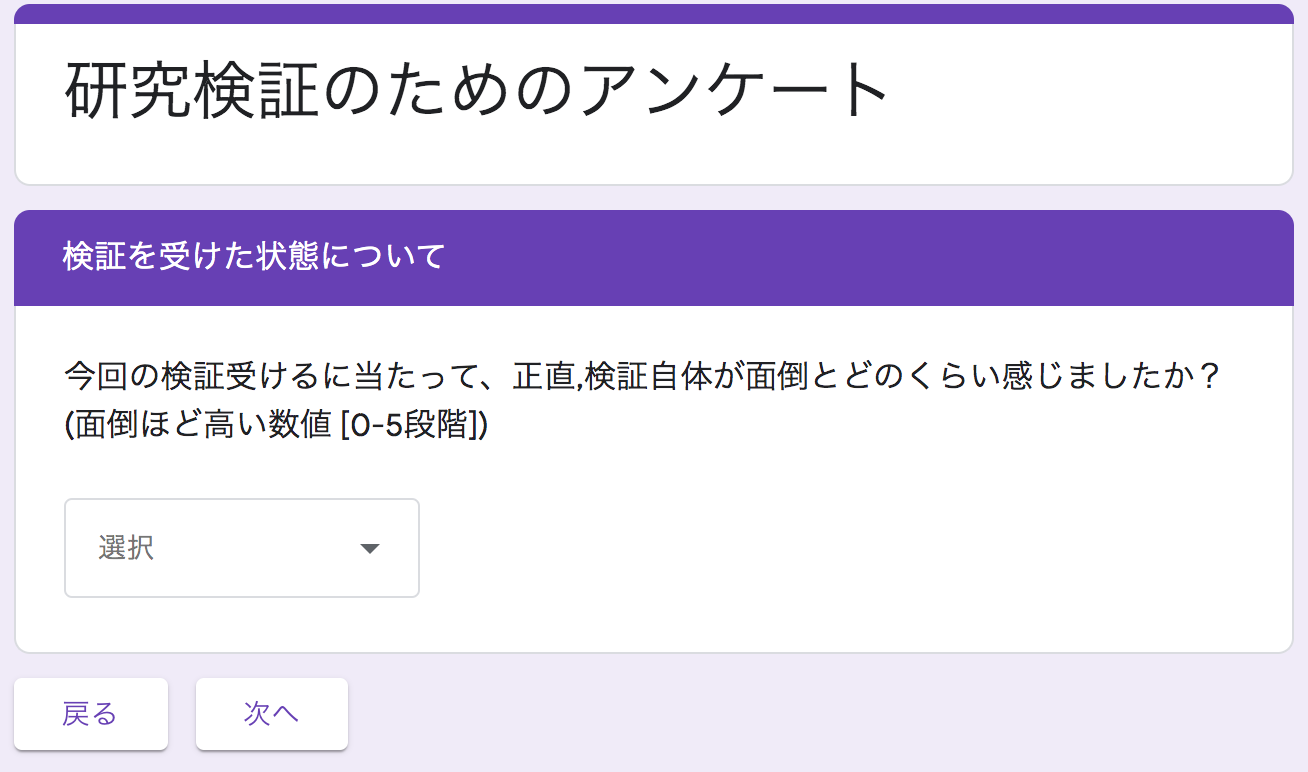
\includegraphics[width=15cm]{./fig/chapter4/inspect_1/questionnaire/questionnaire_1.png}
        \caption{アンケート1}
        \label{アンケート1}
    \end{figure}

    \vspace{4cm}%図の位置を正しくする!
    \begin{figure}[H]
        %\centering
        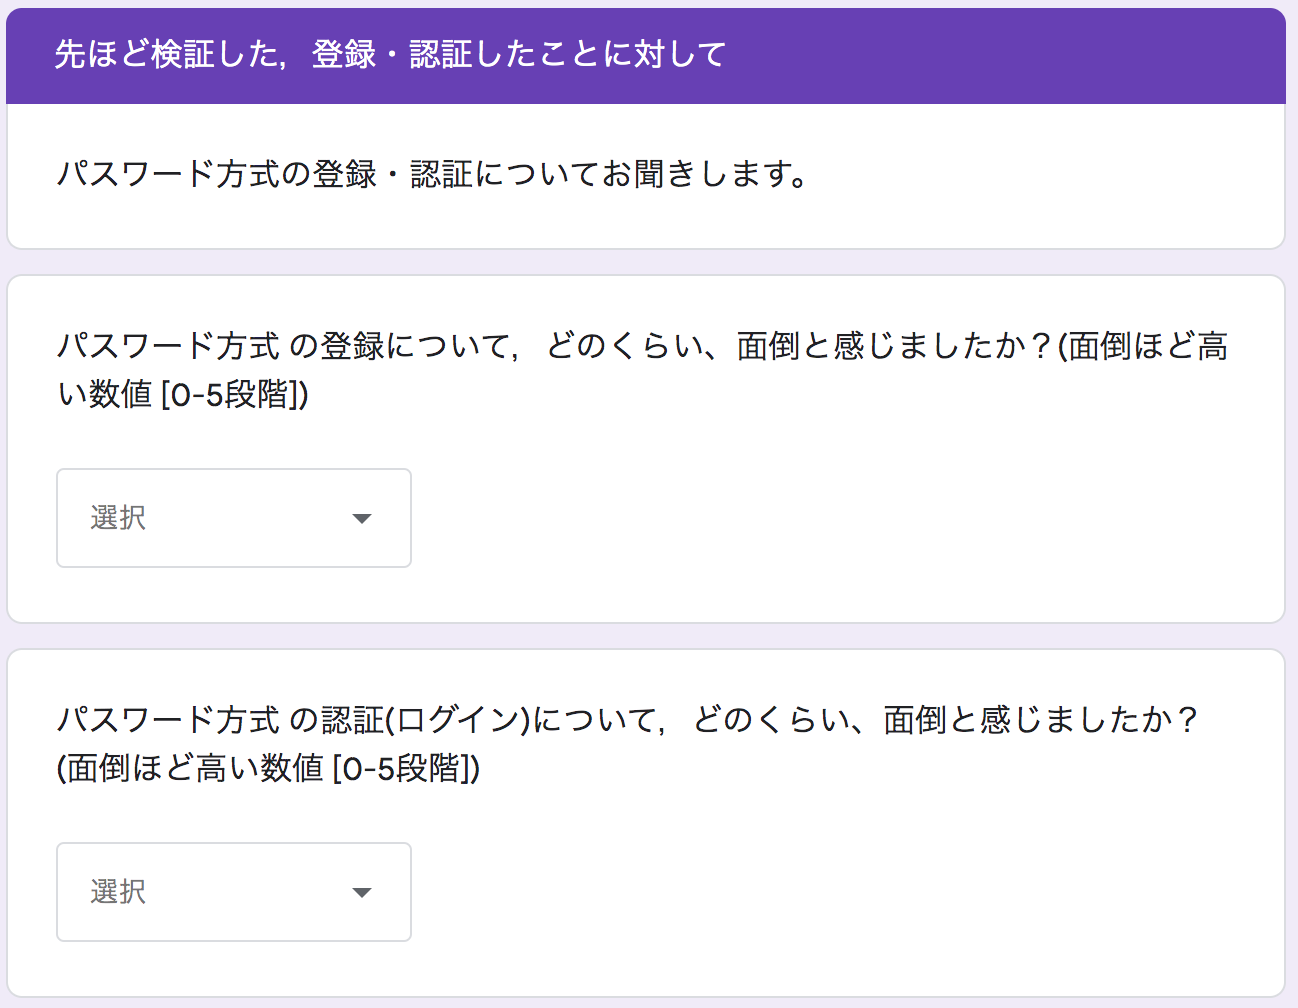
\includegraphics[width=15cm]{./fig/chapter4/inspect_1/questionnaire/questionnaire_2.png}
        \caption{アンケート2}
        \label{アンケート2}
    \end{figure}

    \vspace{4cm}%図の位置を正しくする!
    \begin{figure}[H]
        %\centering
        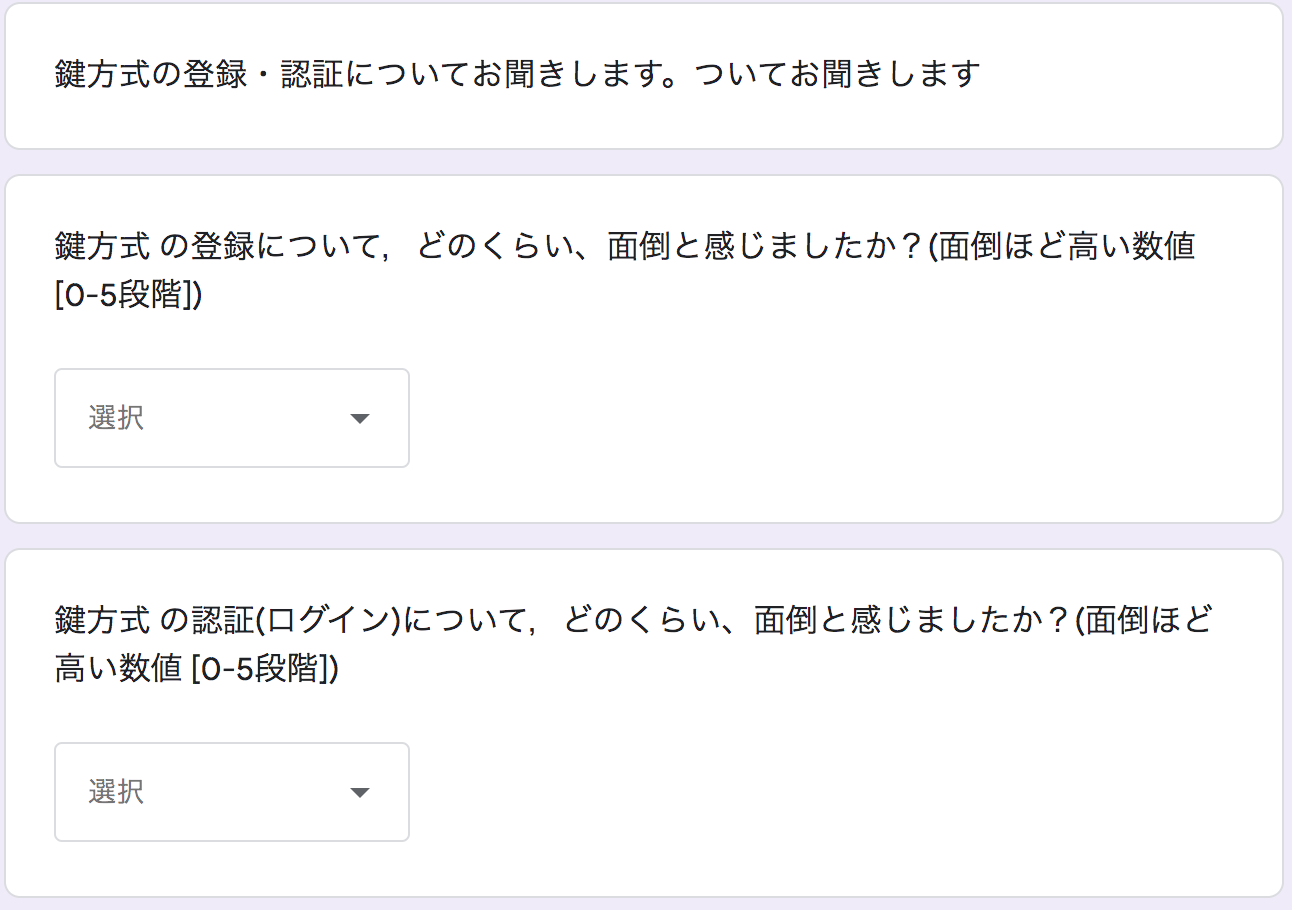
\includegraphics[width=15cm]{./fig/chapter4/inspect_1/questionnaire/questionnaire_3.png}
        \caption{アンケート3}
        \label{アンケート3}
    \end{figure}

    \vspace{4cm}%図の位置を正しくする!
    \begin{figure}[H]
        %\centering
        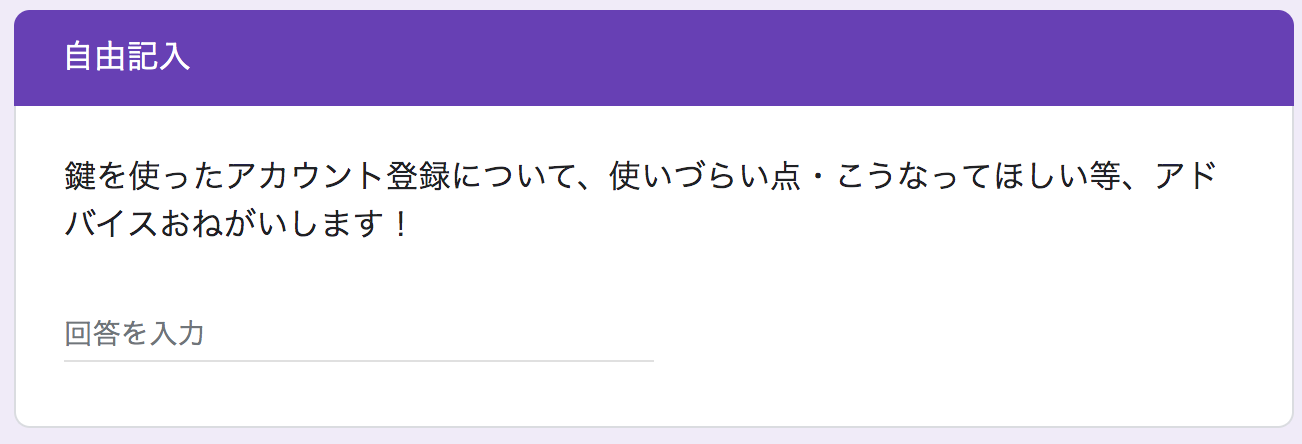
\includegraphics[width=15cm]{./fig/chapter4/inspect_1/questionnaire/questionnaire_4.png}
        \caption{アンケート4}
        \label{アンケート4}
    \end{figure}

    
    % アンケートのスクショ----------------------------------

    %実際に記述--------------------------------------------------------
    




    %%%%%%%%%%%%%%%%%%%%%%%%%%%アン
    %目的
    %  ここでは,被験者に行ったもらう検証画面をのせる。
    %  %(なぜか --> 
    %  % - 検証結果が,どういう検証をした上での,結果になったかを見る必要がある。
    %  % - プラスアルファ
    %  %   - 検証結果を受けて,変更したから,どういう変更したかを,被験者目線でわかるようにする
    %  %)
    %  
    %検証の詳細
    %  パスワード方式の認証・登録の検証画面
    %  鍵方式の認証・登録の検証画面
    %  アンケートの画面
    %
    %  
    %被験者に検証してもらう,鍵方式とパスワード方式それぞれの,登録・認証をする上での,図を載せる。
    %
    %%%%%%%%%%%%%%%%%%%%%%%%%%%アン

 \subsubsection{検証マニュアル}
 %再現性のためにという説明をする
 以下の図\ref{検証マニュアル1},図\ref{検証マニュアル2}は,上記の図\ref{検証1アカウント作成(パスワード方式)} 〜 図\ref{アンケート4} 
 の検証を行うためのマニュアルである.
 マニュアルを作成して,検証を行った意図としては,再現性を持って検証を行うためである.

 \newpage

 \vspace{4cm}%図の位置を正しくする!
 \begin{figure}[H]
     %\centering
     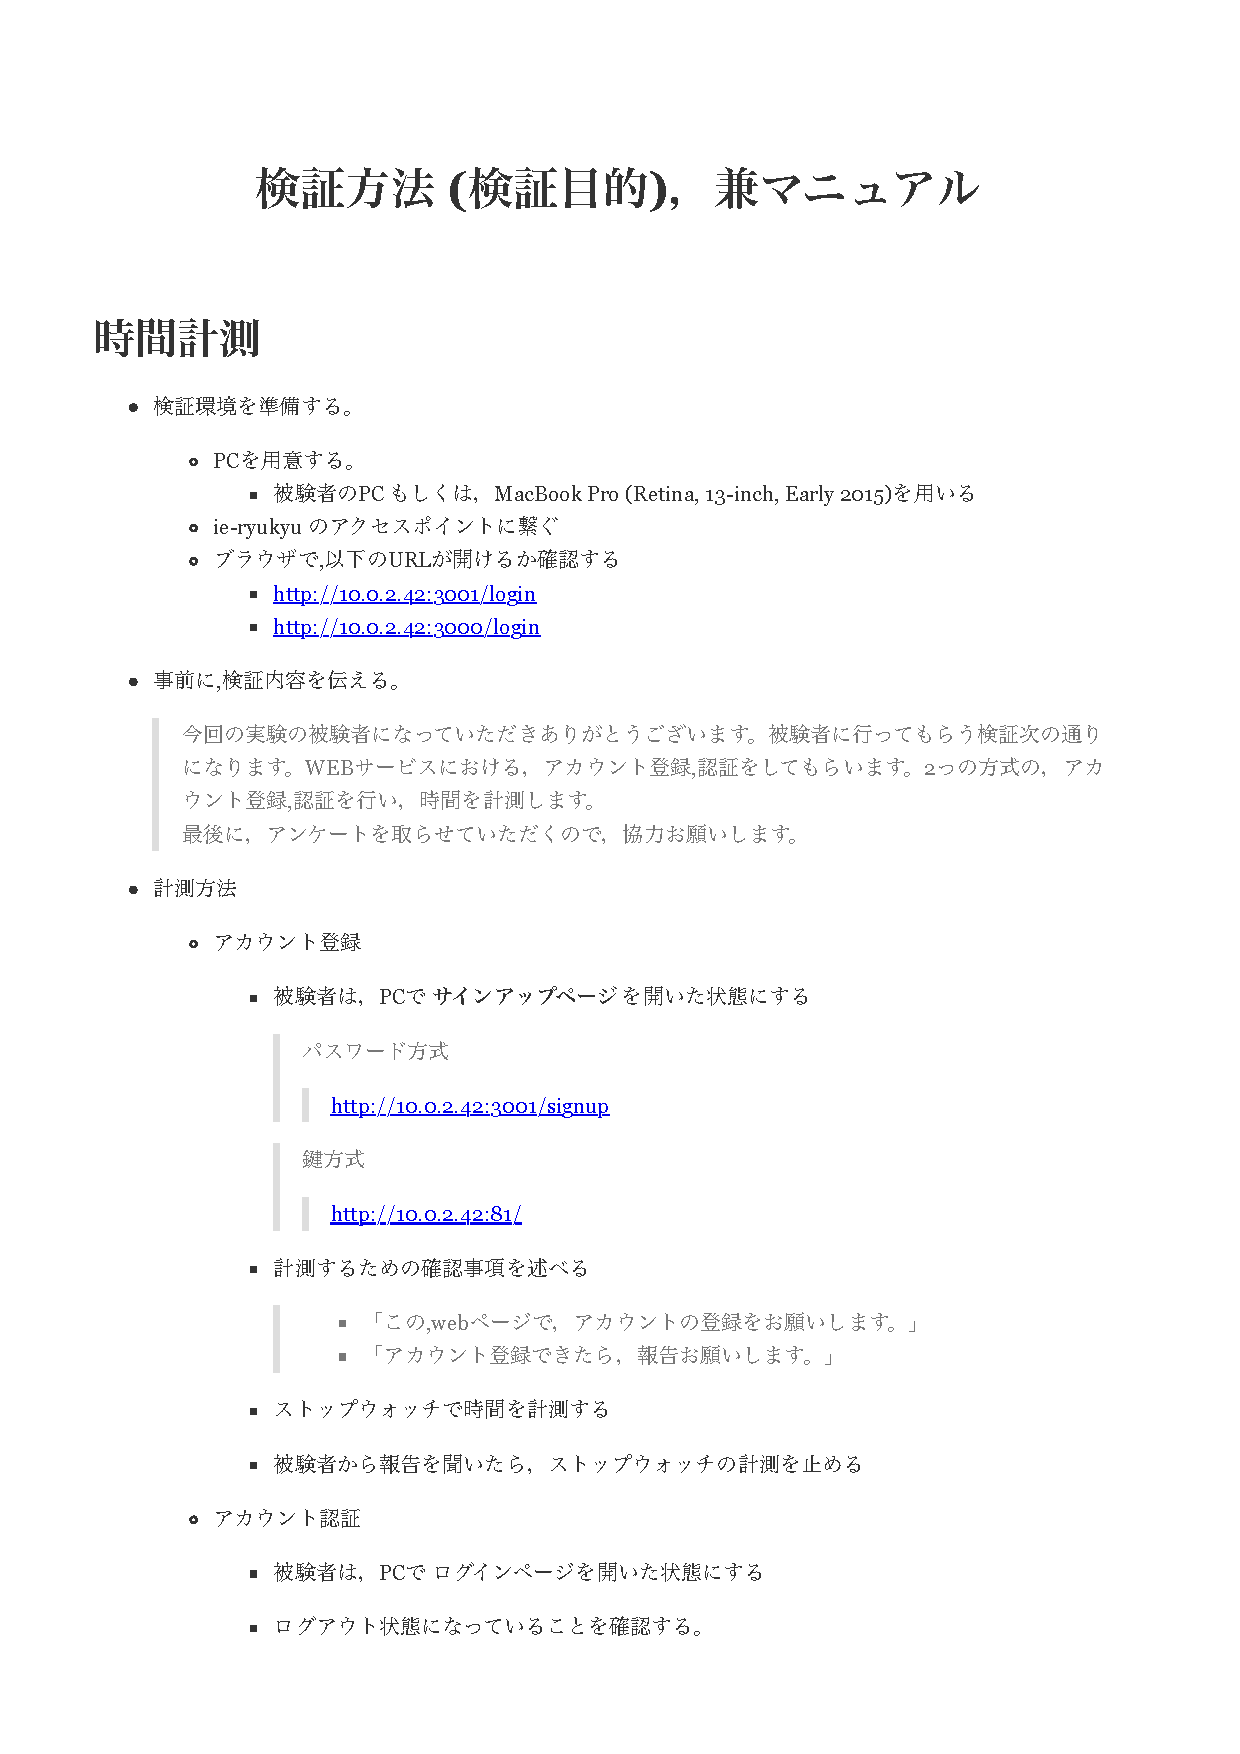
\includegraphics[width=15cm]{./fig/chapter4/inspect_1/manual/manual_1.pdf}
     \caption{検証マニュアル1}
     \label{検証マニュアル1}
 \end{figure}

 \vspace{4cm}%図の位置を正しくする!
 \begin{figure}[H]
     %\centering
     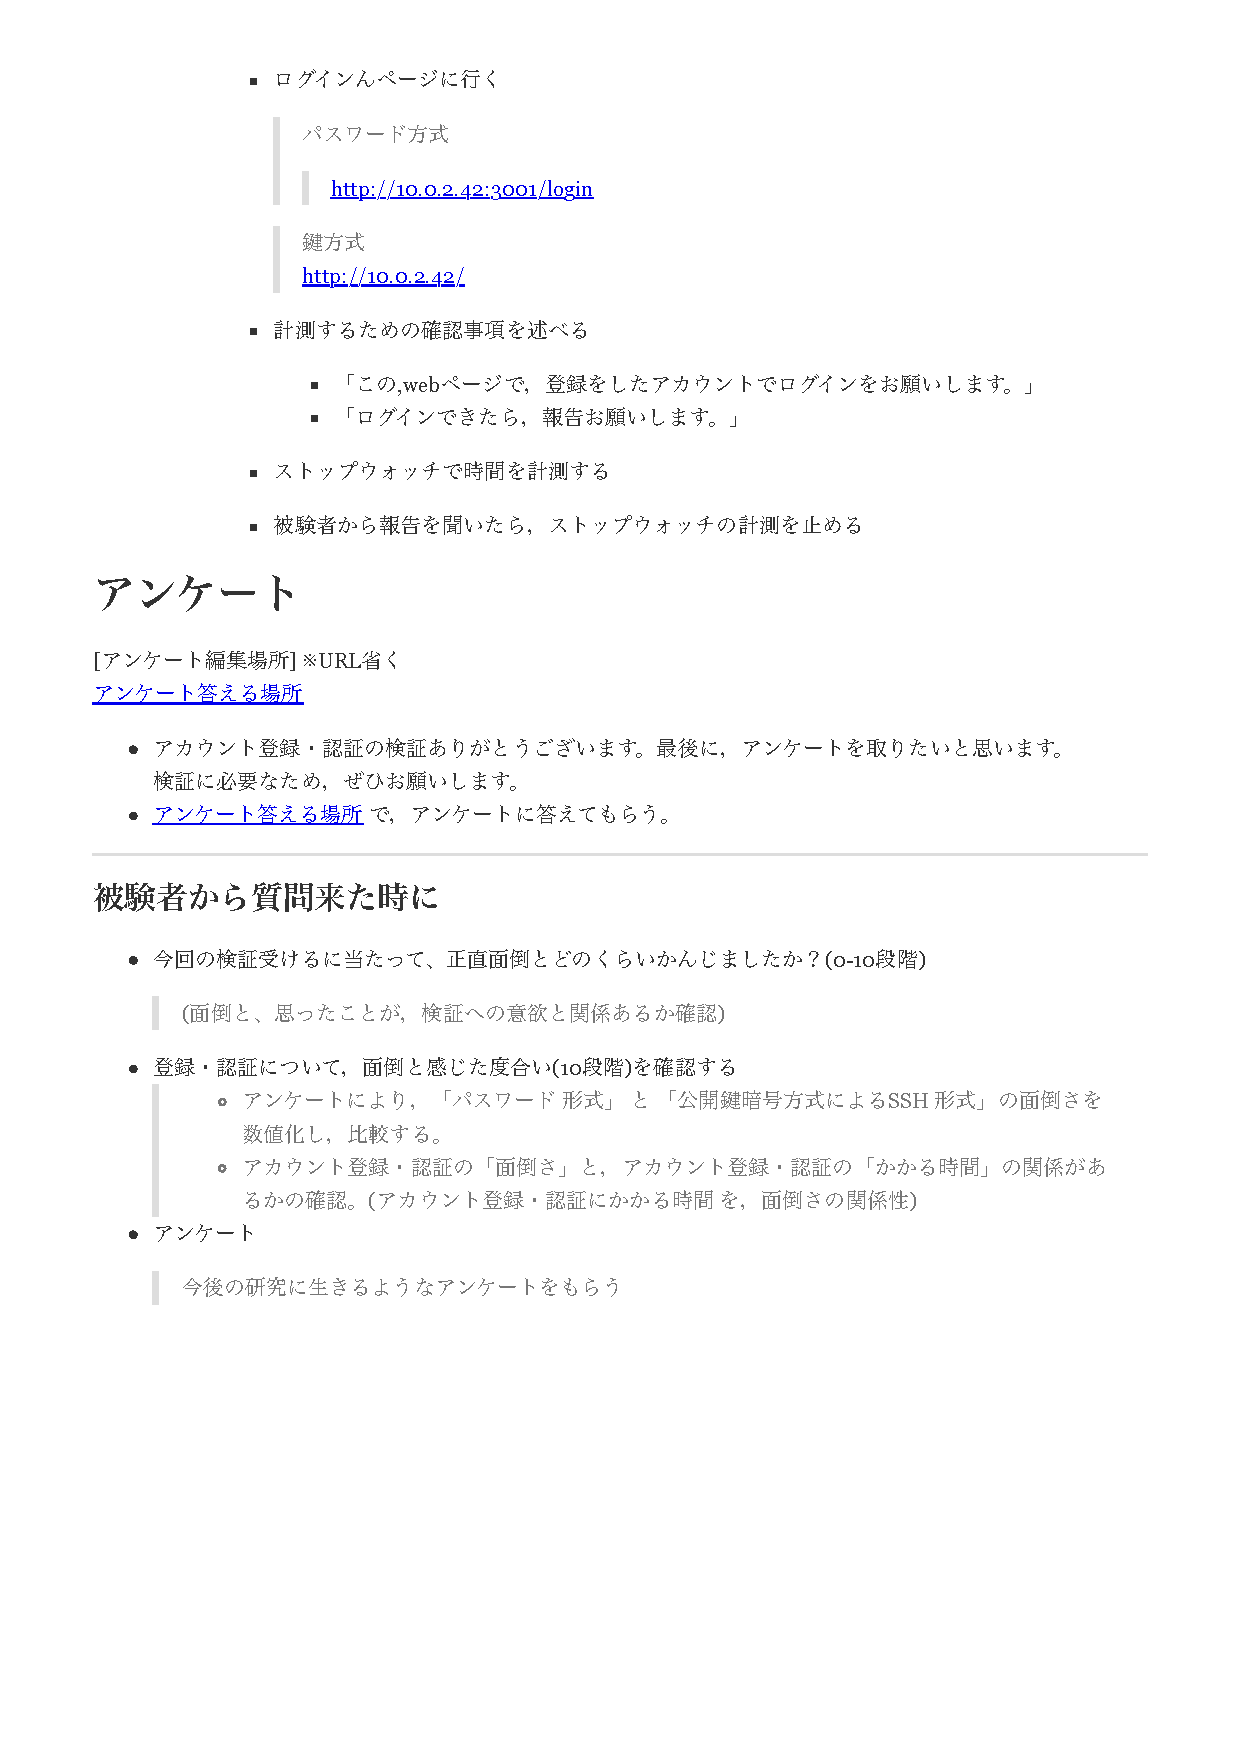
\includegraphics[width=15cm]{./fig/chapter4/inspect_1/manual/manual_2.pdf}
     \caption{検証マニュアル2}
     \label{検証マニュアル2}
 \end{figure}

 \subsection{検証結果}

    \subsubsection{被験者について}
    \begin{itemize}
        \item 琉球大学情報工学科の学生(4人)
    \end{itemize}


    \subsubsection{時間の観点からの面倒さ}
        ここでは被験者に行ってもらった,登録・認証にかかる時間を以下の表\ref{検証1 認証・登録の計測時間}に示す.
        表\ref{検証1 認証・登録の計測時間} は パスワード方式,鍵方式の登録・認証それぞれについて,個の時間,平均時間を記述した表である.
        %表の記述
        \begin{table}[htb]
            \caption{検証1\_認証・登録の計測時間}
            \label{検証1 認証・登録の計測時間}
            \begin{tabular}{|l|r|r|r|r|r|} \hline%| (ハイプ) は縦線
                %登録・認証の種類 \textbackslash 被験者 & 被験者1 & 被験者2 & 被験者3  & 被験者4 & 平均\\ \hline%\hline は横の線
                                & 被験者1 & 被験者2 & 被験者3  & 被験者4 & 平均 \\ \hline%\hline は横の線
                登録(パスワード方式) & 24.88 & 38.99 & 28.21 & 18.04 & 27.53 \\ \hline
                認証(パスワード方式) & 16.57 & 13.24 & 21.27 & 12.23 & 15.83 \\ \hline
                登録(鍵方式)       & 19.96 & 19.14 & 21.73 & 7.81 & 17.16 \\ \hline
                認証(鍵方式)       & 14.86 & 18.63 & 18.35 & 11.47 & 15.83 \\ \hline

                %----- 最終ページの表の最下部 --------
                \multicolumn{6}{r}{\small\it (単位:秒)}\\
                \end{tabular}
        \end{table}

        %上の表の参考方法
        %%表\ref{検証1 認証・登録の計測時間}

    \subsubsection{アンケートの観点からの面倒さ}
        ここでは,被験者に対して,2つの方式の登録・認証が終わった直後に,
        記入してもらったアンケートについての数値のまとめを以下の表\ref{検証1 アンケートによる6段階評価}に示す.
        表\ref{検証1 アンケートによる6段階評価}は 被験者による パスワード方式,鍵方式の登録・認証それぞれについて0 〜 5 段階評価,さらに,検証自体の面倒さについての評価を加えて まとめた表である.
        %表の記述
        \begin{table}[htb]
            \caption{検証1\_アンケートによる6段階評価}
            \label{検証1 アンケートによる6段階評価}
            \begin{tabular}{|l|r|r|r|r|r|} \hline%| (ハイプ) は縦線
                %登録・認証の種類 \textbackslash 被験者 & 被験者1 & 被験者2 & 被験者3  & 被験者4 & 平均\\ \hline%\hline は横の線
                                        & 被験者1 & 被験者2 & 被験者3  & 被験者4 & 平均 \\ \hline%\hline は横の線
                登録(パスワード方式)の面倒さ & 1 & 1 & 2 & 0 & 1 \\ \hline
                認証(パスワード方式)の面倒さ & 1 & 1 & 2 & 1 & 1.25 \\ \hline
                登録(鍵方式)の面倒さ       & 0 & 2 & 0 & 1 & 0.75 \\ \hline
                認証(鍵方式)の面倒さ       & 0 & 2 & 0 & 2 & 1 \\ \hline
                検証自体の面倒さ       & 2 & 1 & 1 & 1 & 1.25 \\ \hline
    
                %----- 最終ページの表の最下部 --------
                \multicolumn{6}{r}{\small\it (0 〜 5段階)}\\
            \end{tabular}
        \end{table}

        %上の表の参考方法
        %%表\ref{検証1 アンケートによる6段階評価}

 \newpage


 \subsection{考察}
 時間の観点での"面倒さ"では,時間がかかる方"面倒"と感じると予測していたため,
 パスワードの観点と,アンケートの観点の面倒さの数値は比例すると考えていた。
 しかし,表\ref{検証1 認証・登録の計測時間},表\ref{検証1 アンケートによる6段階評価} 被験者2の
 パスワード方式と鍵方式の「アカウント登録・認証にかかる時間の大きさ」と,
 「アンケートによる面倒の数値」が,半比例関係だった.
 上記のような結果になった理由としては2通り考えられる.
 1つ目は,普段登録,認証で使っている,パスワード方式の方が,慣れているため,「面倒」と感じにくかったと考察することができる.
 2つ目は,アンケートに「PCから秘密鍵を選択するのが少し面倒だと感じた。」とあり,鍵の管理を面倒だと感じたことが,影響したと思われる.

 鍵方式についてのアンケートの結果に「なんかわかった」というアンケートの記述があった.
 被験者に確認したところ,鍵方式の登録・認証の流れがよく分からなかったとのことだった.
 実際に,鍵方式で登録する際に,登録できたのか戸惑っていた。
 この原因としては,鍵方式の登録・認証の流れが分からなかったためだと考えられる.

 表\ref{検証1 アンケートによる6段階評価}の検証自体の面倒さは0数値にする人が無く,
 検証自体に,少しながら面倒と感じていることが分かる.
 その原因としては,検証するためのWEBページ(図\ref{検証1アカウント作成(パスワード方式)} 〜 図\ref{検証1認証成功後(鍵方式)} )が
 デバッグページのままで,登録・認証が作業的になってしまったためだと考えられる.

 検証後の聞き取りで,パスワード方式の登録で以下のような日常的に,
 使用しないと思われるパスワードの確認ができた.
 \begin{itemize}
    \item パスワードの使い回し
    \item パスワード "password"を設定する
 \end{itemize}
 そのことから,検証方法のマニュアルに,
 普段使うようなWEBサービスのように実施してもらうような注意事項を用意する必要がある.

\newpage





%% 検証2でやるやつ
%\section{検証2}
%  \subsection{検証背景}
%    \subsubsection{検証目的}
%    \subsubsection{検証手段} 
%  \subsection{検証環境}                        OK
%    \subsubsection{検証場所}                   OK
%    \subsubsection{検証の流れ}                 OK
%    \subsubsection{検証画面}                   OK
%    \subsubsection{検証マニュアル}              OK
%  \subsection{検証結果}
%  \subsection{考察}




\section{検証2}
  \subsection{検証背景}
    \subsubsection{検証目的}
    password認証方式の,新規登録・認証の面倒さを解決するために,第3章の提案手法で
    password認証方式に変わる,公開鍵暗号方式によるssh認証を用いた,WEBサービス認証の提案を行った。\\
    しかしながら,提案だけだと,新規登録・認証の面倒さを解決していることの根拠に乏しい。
    よって,検証を行い,第3章の提案手法は"面倒さの軽減"に効果的に繋がっているかの確認をする。
    \subsubsection{検証手段} 
    検証の手段としては,実際に,以下の2つの認証方式の登録・認証を被験者に体験してもらう。
    %また,実験マニュアルを作成し,実験者は被験者に対して,同じように接するようにする。

    \begin{itemize}
    \item パスワード方式認証(以後 "パスワード認証"と記述する)
    \item 公開鍵暗号暗号方式によるssh認証(以後 "鍵認証”と記述する)
    \end{itemize}

    その後,2つの観点から,"面倒さ"を数値化する。
    1つ目の観点は「時間」である。
    "面倒さ"をアカウント登録・認証にかかる時間と推測し,計測化する。
    詳しい詳細については,検証環境のマニュアルに記述する。
    %まず,パスワード 形式による登録・認証の時間計測をそれぞれ行う。
    % 次に,公開鍵暗号方式によるSSH 形式登録・認証の時間計測をそれぞれ行う。
    % 最後に,上記の形式による時間計測を比較する。
    2つ目の観点は「アンケート」である。
    アンケートには,点数で答える方式,文字で記入する欄 の2つがあり,点数で答える方式により"面倒さ”を数値化する。
    アンケートの細かい内容は,4.1.3の検証画面に記述する。

    また,アンケートには"面倒さ"を数値化する以外にも,以下の2つの意味を込める。
    1つ目の意味は次の通りである。
    アカウント登録・認証にかかる時間 を,"面倒さ"と予想して検証しているが,その予想を確かめる必要がある。
    アンケートを取ることにより,「アカウント登録・認証にかかる時間」と,「アンケートによる面倒さ」が比例していることを確認することで,予想を確かめることができる。
    また,被験者の状態も確認することで,面倒と感じるのが,検証自体に対しての面倒さと関係があるのかを確認する。
    2つ目の意味は次のとおりである。
    記入欄で,改善点や感じたことの意見をもらうことで,今後の研究に生きるようなアンケートをもらう。

    検証1より効果的な検証方法にするため変更して検証をおこなう.変更点とその理由についてはそれぞれの項で述べる.

  \newpage

  \subsection{検証環境} 
    \subsubsection{検証場所}% 基本一緒?
       第3章で記述したとおり,検証場所は学科のVMを用いているため,学科のネットワーク内(有線LAN,wifiアクセスポイント{ie-ryukyu})
        から,アクセスして検証を行う。
    \subsubsection{検証の流れ}% 基本一緒?
        ここでは,被験者に行ってもらう,検証の流れを記述する。
        時間の観点で"面倒さ"を数値化する検証では,被験者にはパスワード方式,鍵方式の登録・認証をそれぞれ行ってもらう。その時,被験者は時間を測る。 
        また,再現性を持って,検証を行うためにマニュアルを作成し,マニュアル通りに検証を行う。
        アンケートの観点で"面倒さ"を数値化する検証では,
        時間の観点で"面倒さ"を数値化する検証 が終わった直後に行うようにすることで,被験者の思った感情とアンケート結果の差異が少なくなるようにする。


    \newpage

    \subsubsection{検証画面}

    ここでは,検証1より効果的に検証結果目的を達成するために,修正した検証2の検証画面とその意図について述べる。

    %ここで,検証を行った際に,検証1と比較して被験者が視覚的・聴覚的に差異が生じる主な変更点を以下に述べる。

    まずは検証画面図の説明をする。\\
    パスワード方式について
    \begin{itemize}
        \item 図\ref{検証2ホーム画面(パスワード方式)}は,ホーム画面である.
        \item 図\ref{検証2アカウント作成(パスワード方式)}は,アカウント登録画面である。
        \item 図\ref{検証2認証(パスワード方式)}は,図\ref{検証2アカウント作成(パスワード方式)}で登録したアカウントに認証するための画面である。
        \item 図\ref{検証2認証成功後(パスワード方式)}は,図\ref{検証2認証(パスワード方式)}で認証成功した後の画面である。
    \end{itemize}
    %
    鍵方式について\\
    \begin{itemize}
        \item 図\ref{検証2ホーム画面(鍵方式)}は,ホーム画面である.
        \item 図\ref{検証2アカウント作成(鍵方式)}は,アカウント登録画面である。
        \item 図\ref{検証2認証(鍵方式)}は,図\ref{検証2アカウント作成(鍵方式)}で登録したアカウントに認証するための画面である。
        \item 図\ref{検証2認証成功後(鍵方式)}は,図\ref{検証2認証(鍵方式)}で認証成功した後の画面である。
    \end{itemize}



    % 言いたいやつ----------------------------------------------------------------------------------------------

    %% web画面面 -----------------------------------------------------
    %%% アンケートの"検証自体面倒"という観点から
    %%%%検証1のアンケートで,"検証自体が面倒"と答える被験者の平均が,5段階中の1であった。その原因として,
    %%%%デバッグ画面や,登録フォーム・認証フォームだけのWEB画面が,
    %%%%作業的な検証に繋がり,”検証自体が面倒"に繋がった大きな要因の一つと考えられる。
    %%%%よって,ホーム画面(図???)の用意や,デバッグの消去(図???),さらには,「幸せになれるWEBサイト」と認識してもらうことで,被験者にとって,作業的な検証から,WEBサービスに登録する検証を狙って,変更した。
    %% web画面面 -----------------------------------------------------

    %% 細かいやつ
    %%%アンケートは検証1と同じ質問(意図)をしているため,割愛する。

    % 言いたいやつ----------------------------------------------------------------------------------------------

    次に,検証1 との変更点と,その意図について述べる。
    %アンケートの"検証自体面倒"という観点から
    検証1のアンケート(図\ref{検証2アカウント作成(鍵方式)})で,"検証自体が面倒"と答える被験者の平均が,5段階中の1であった。その原因として,
    デバッグ画面や,登録フォーム・認証フォームだけのWEB画面が,
    作業的な検証に繋がり,"検証自体が面倒"に繋がった大きな要因の一つと考えられる。
    よって,ホーム画面(図\ref{検証2ホーム画面(パスワード方式)},図\ref{検証2ホーム画面(鍵方式)})の用意や,
    デバッグのための文字の消去(図\ref{検証2アカウント作成(パスワード方式)} 〜 図\ref{検証2認証成功後(パスワード方式)} , \ref{検証2アカウント作成(鍵方式)} 〜 \ref{検証2アカウント作成(鍵方式)}),
    さらには,「幸せになれるWEBサイト」( 図\ref{検証2ホーム画面(パスワード方式)} 〜 \ref{検証2アカウント作成(鍵方式)} )と認識してもらうことで,
    被験者にとって,作業的な検証から,WEBサービスに登録する検証になることを狙って,変更した。









    % パスワード方式のスクショ---------------------------
    \vspace{4cm}%図の位置を正しくする!
    %\begin{figure}[h]
    \begin{figure}[H]
        %\centering
        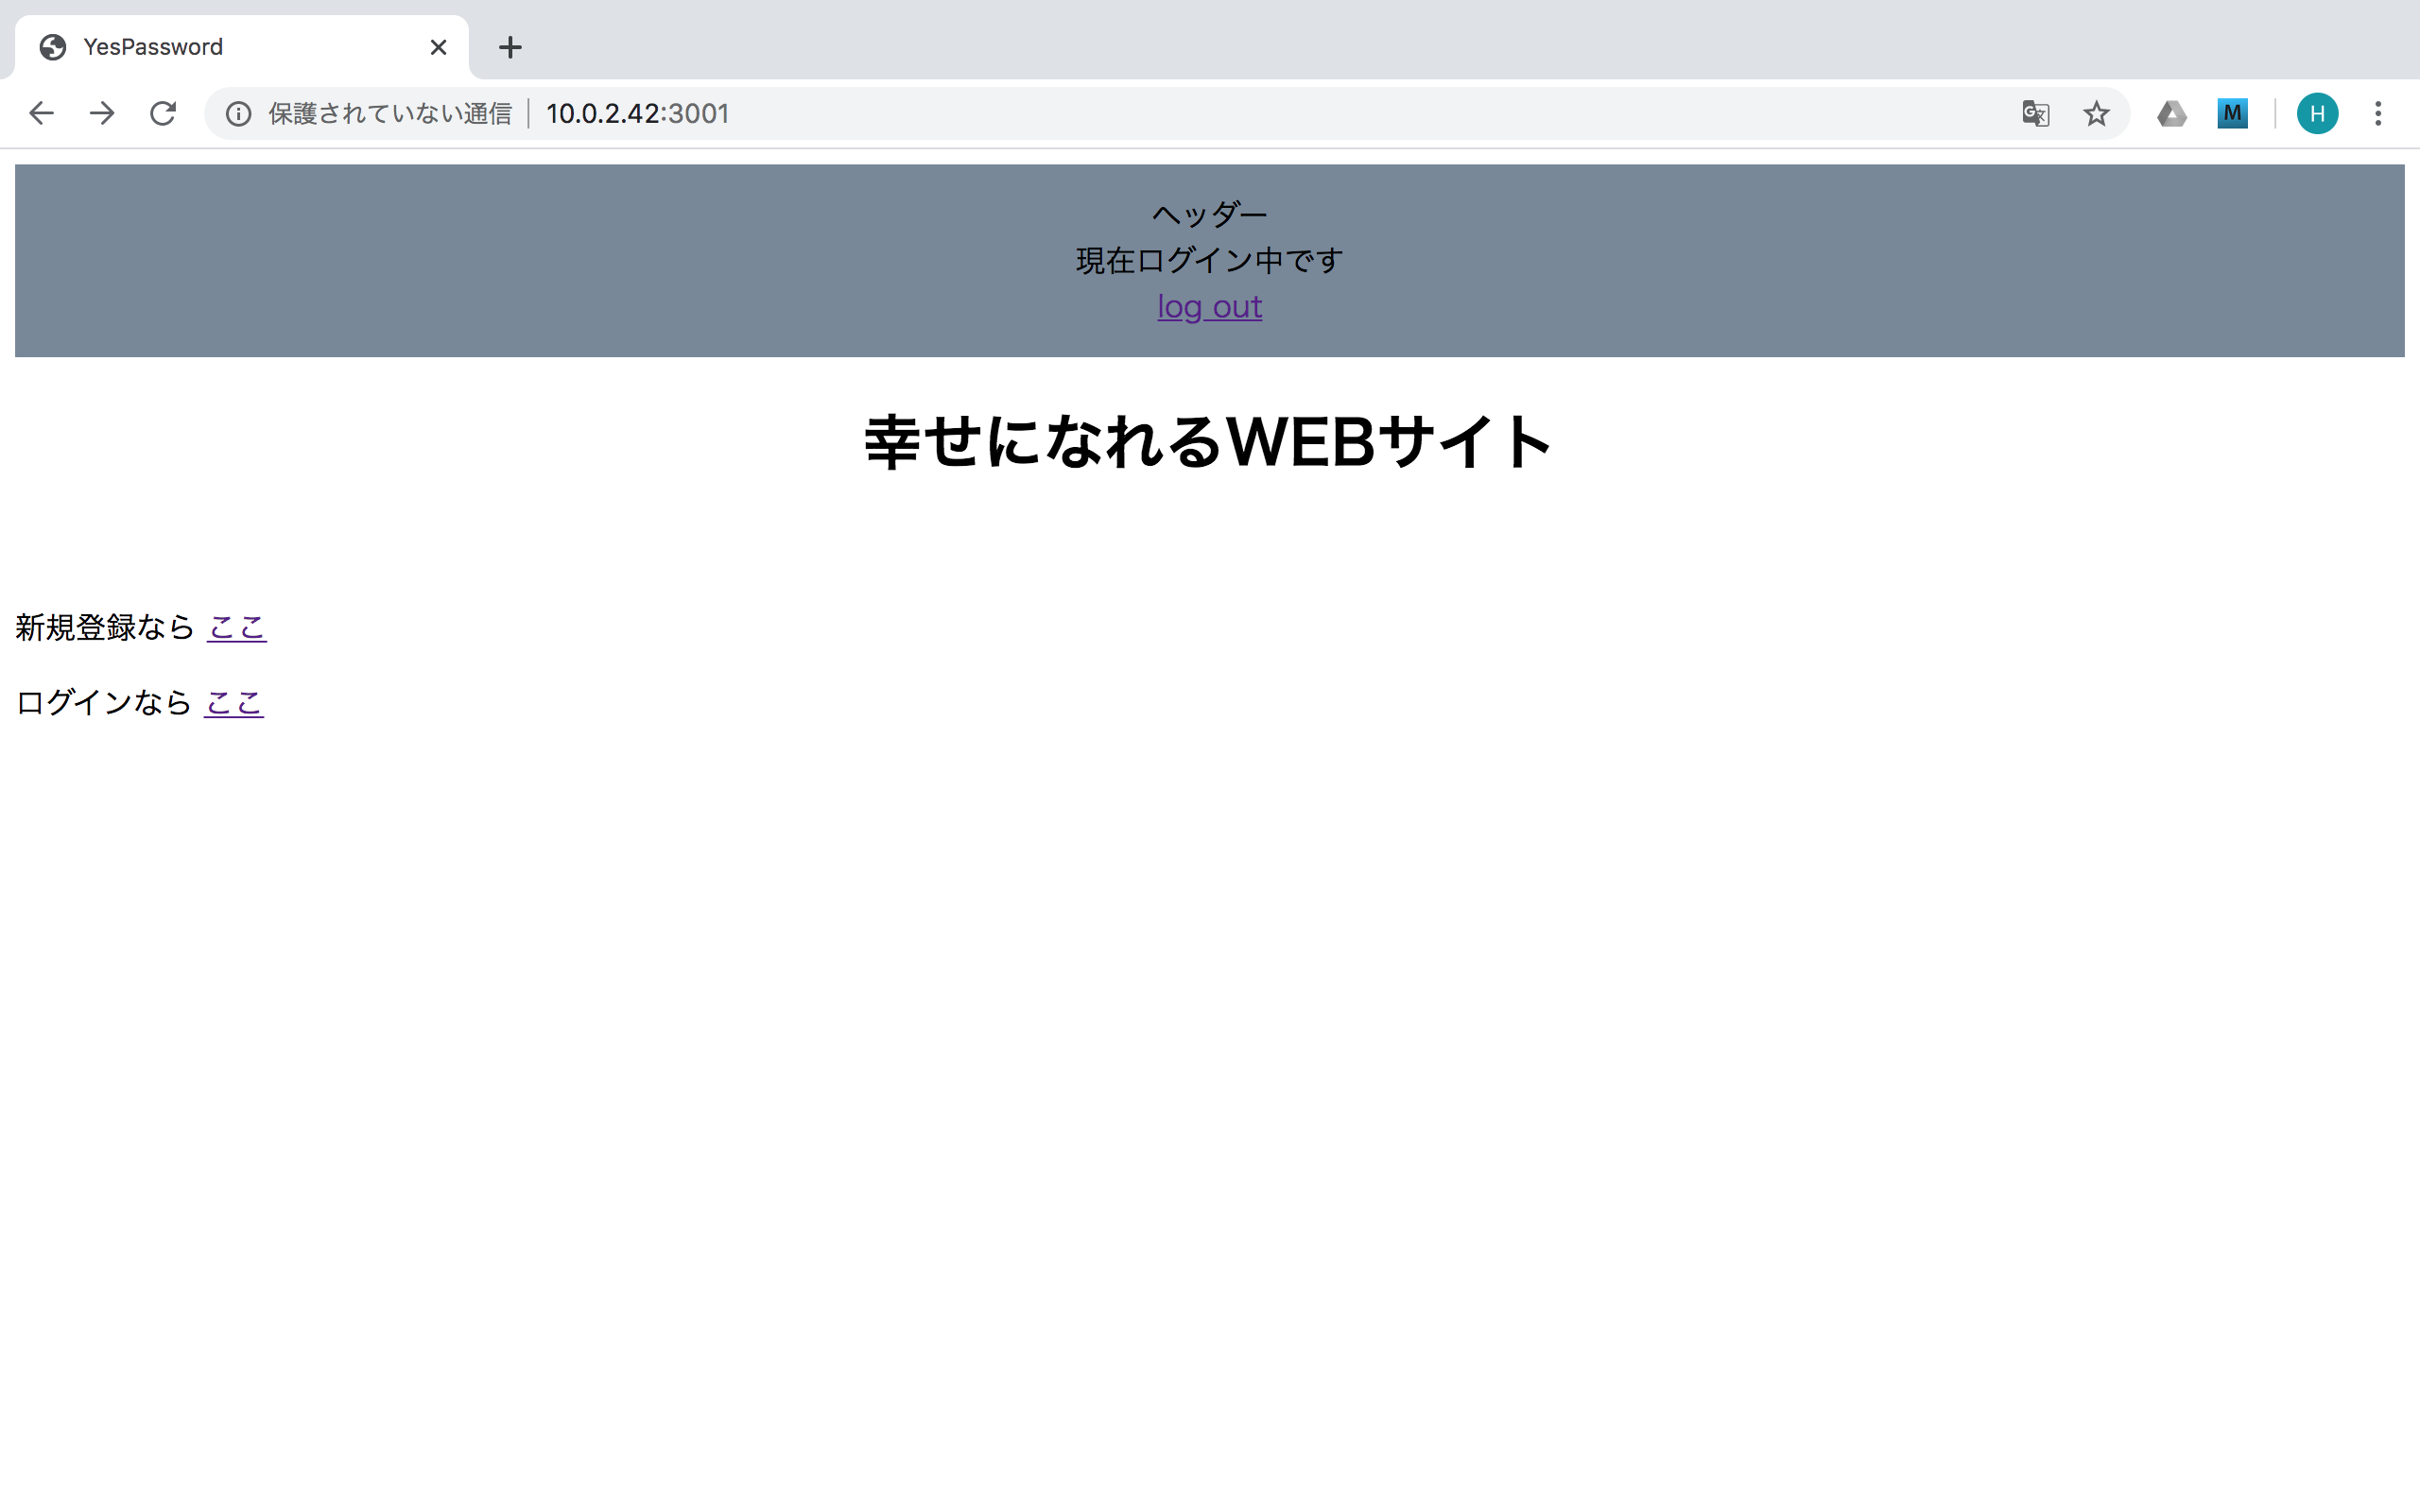
\includegraphics[height=8.4cm]{./fig/chapter4/inspect_2/password_screnn/home.png}
        \caption{検証2\_ホーム画面(パスワード方式)}
        \label{検証2ホーム画面(パスワード方式)}
    \end{figure}


    \vspace{4cm}%図の位置を正しくする!
    %\begin{figure}[h]
    \begin{figure}[H]
        %\centering
        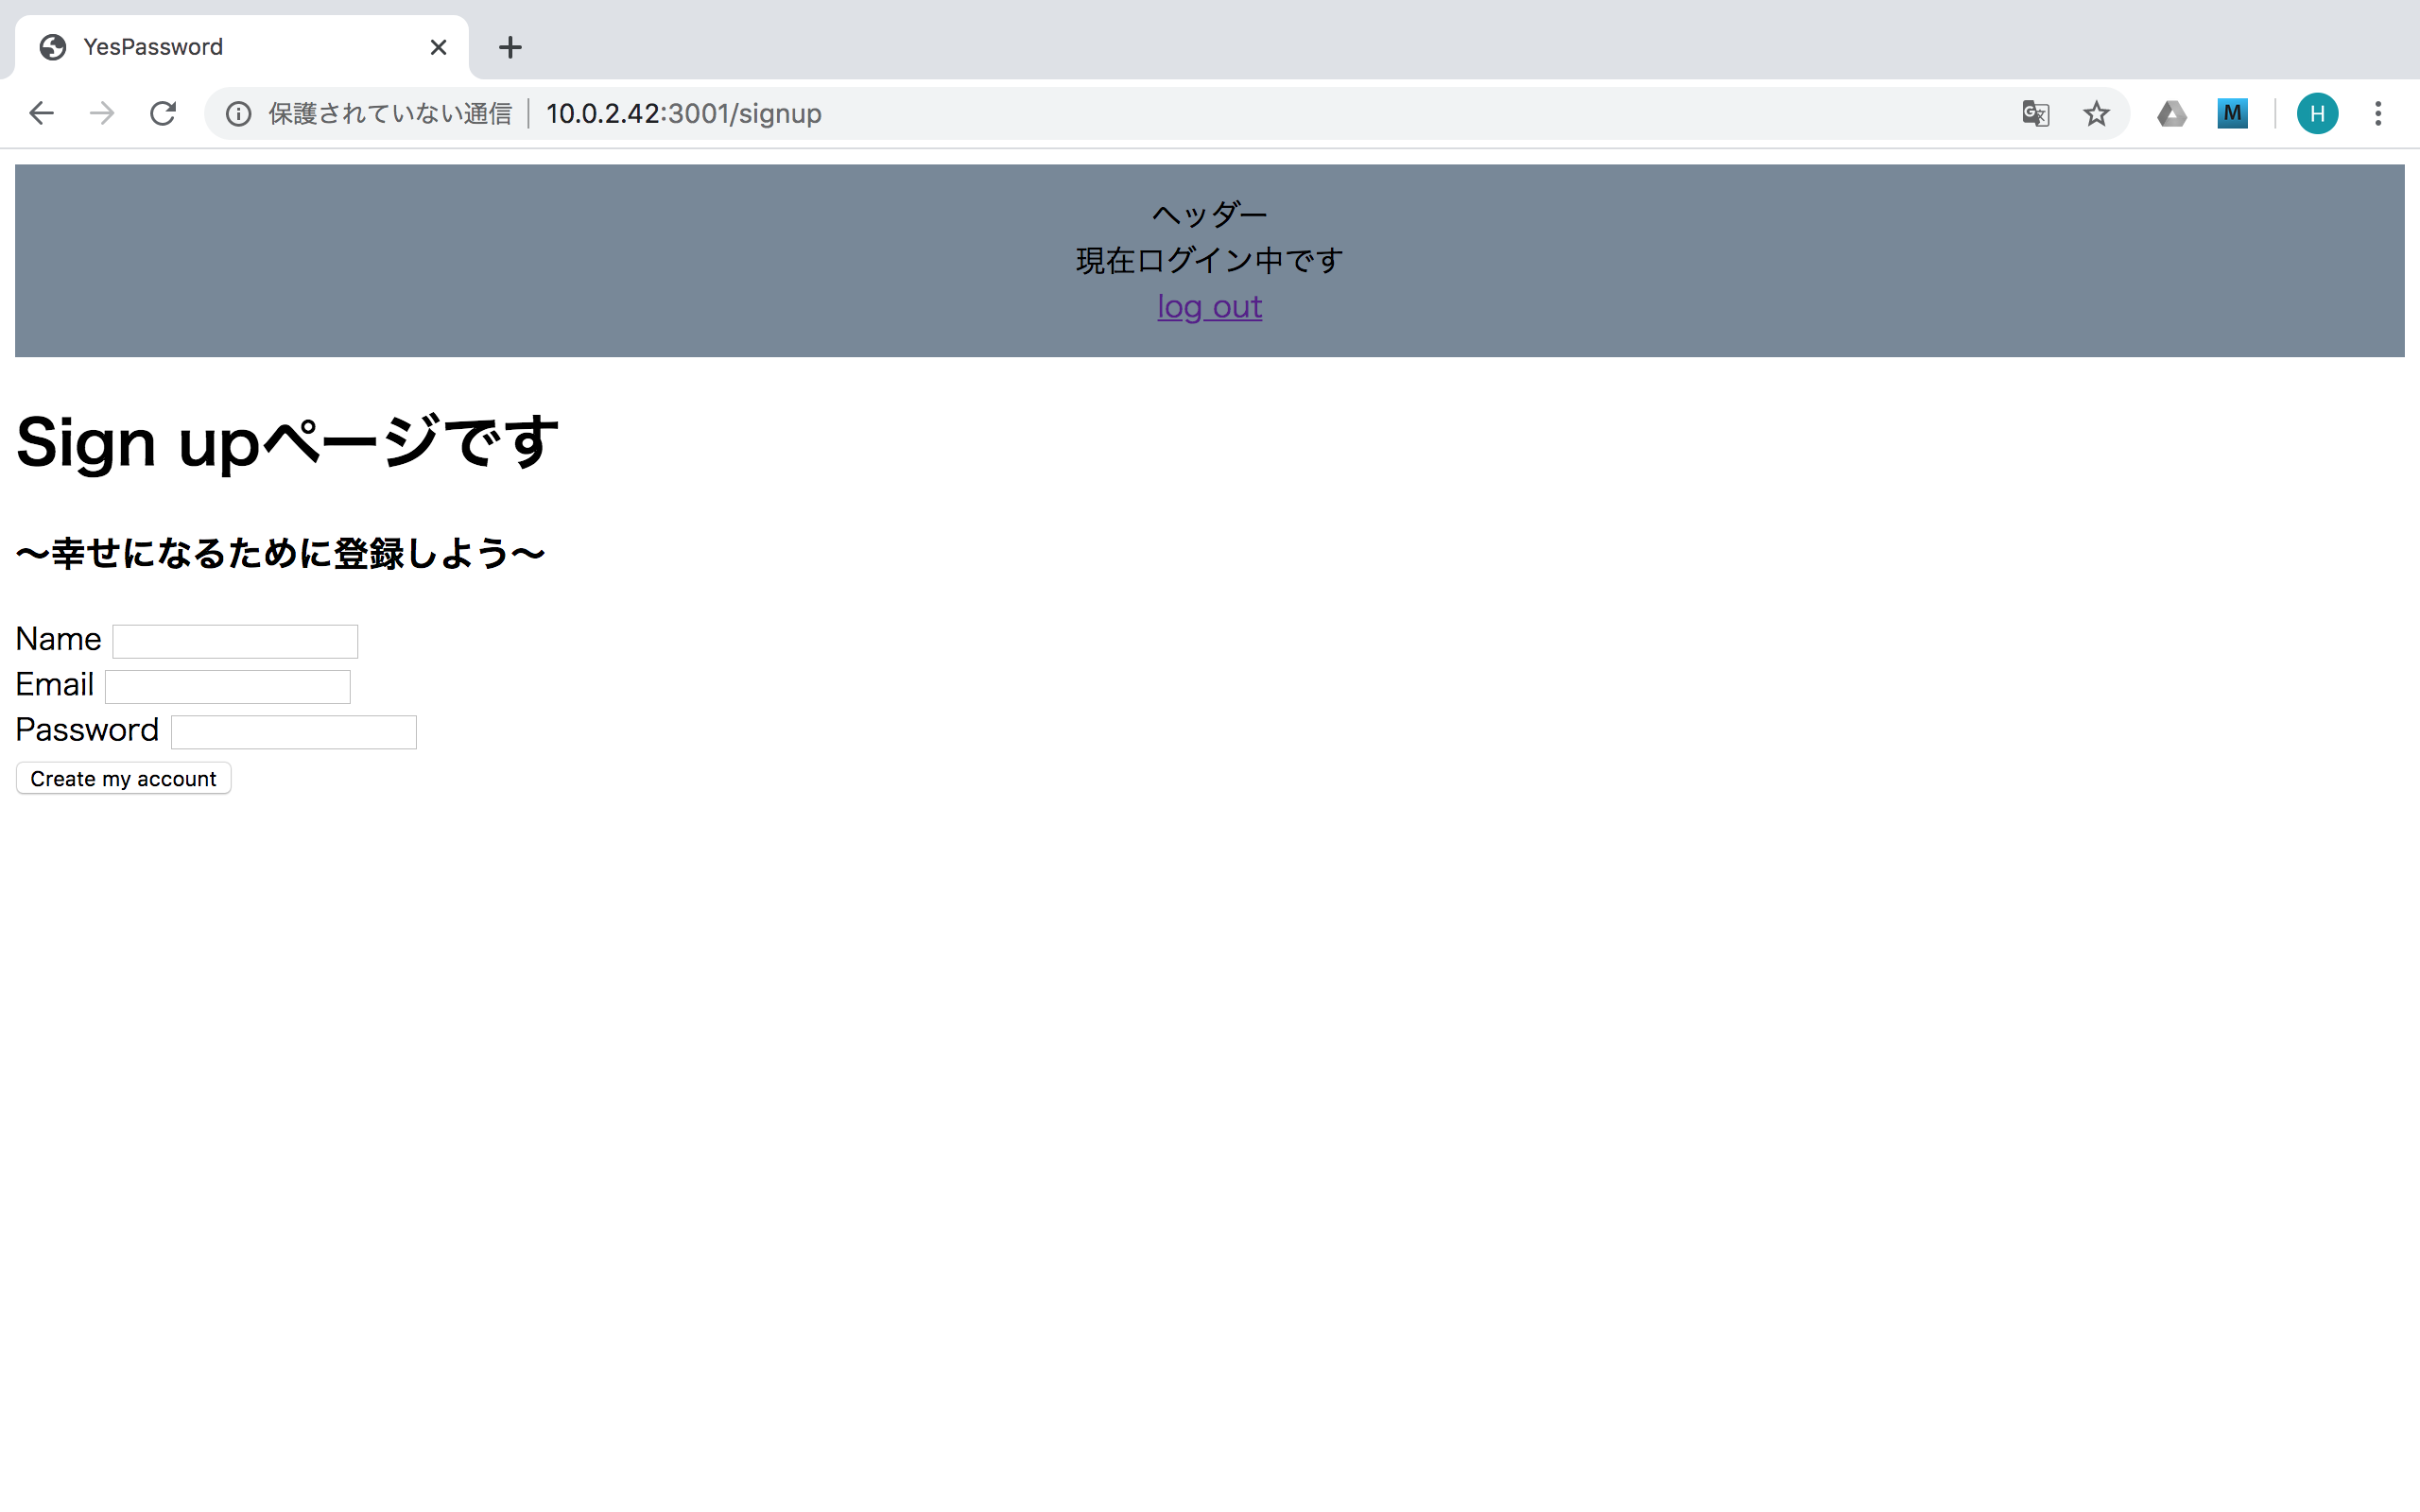
\includegraphics[height=8.4cm]{./fig/chapter4/inspect_2/password_screnn/sign_up.png}
        \caption{検証2\_アカウント作成(パスワード方式)}
        \label{検証2アカウント作成(パスワード方式)}
    \end{figure}

    \vspace{4cm}%図の位置を正しくする!
    %\begin{figure}[h]
    \begin{figure}[H]
        %\centering
        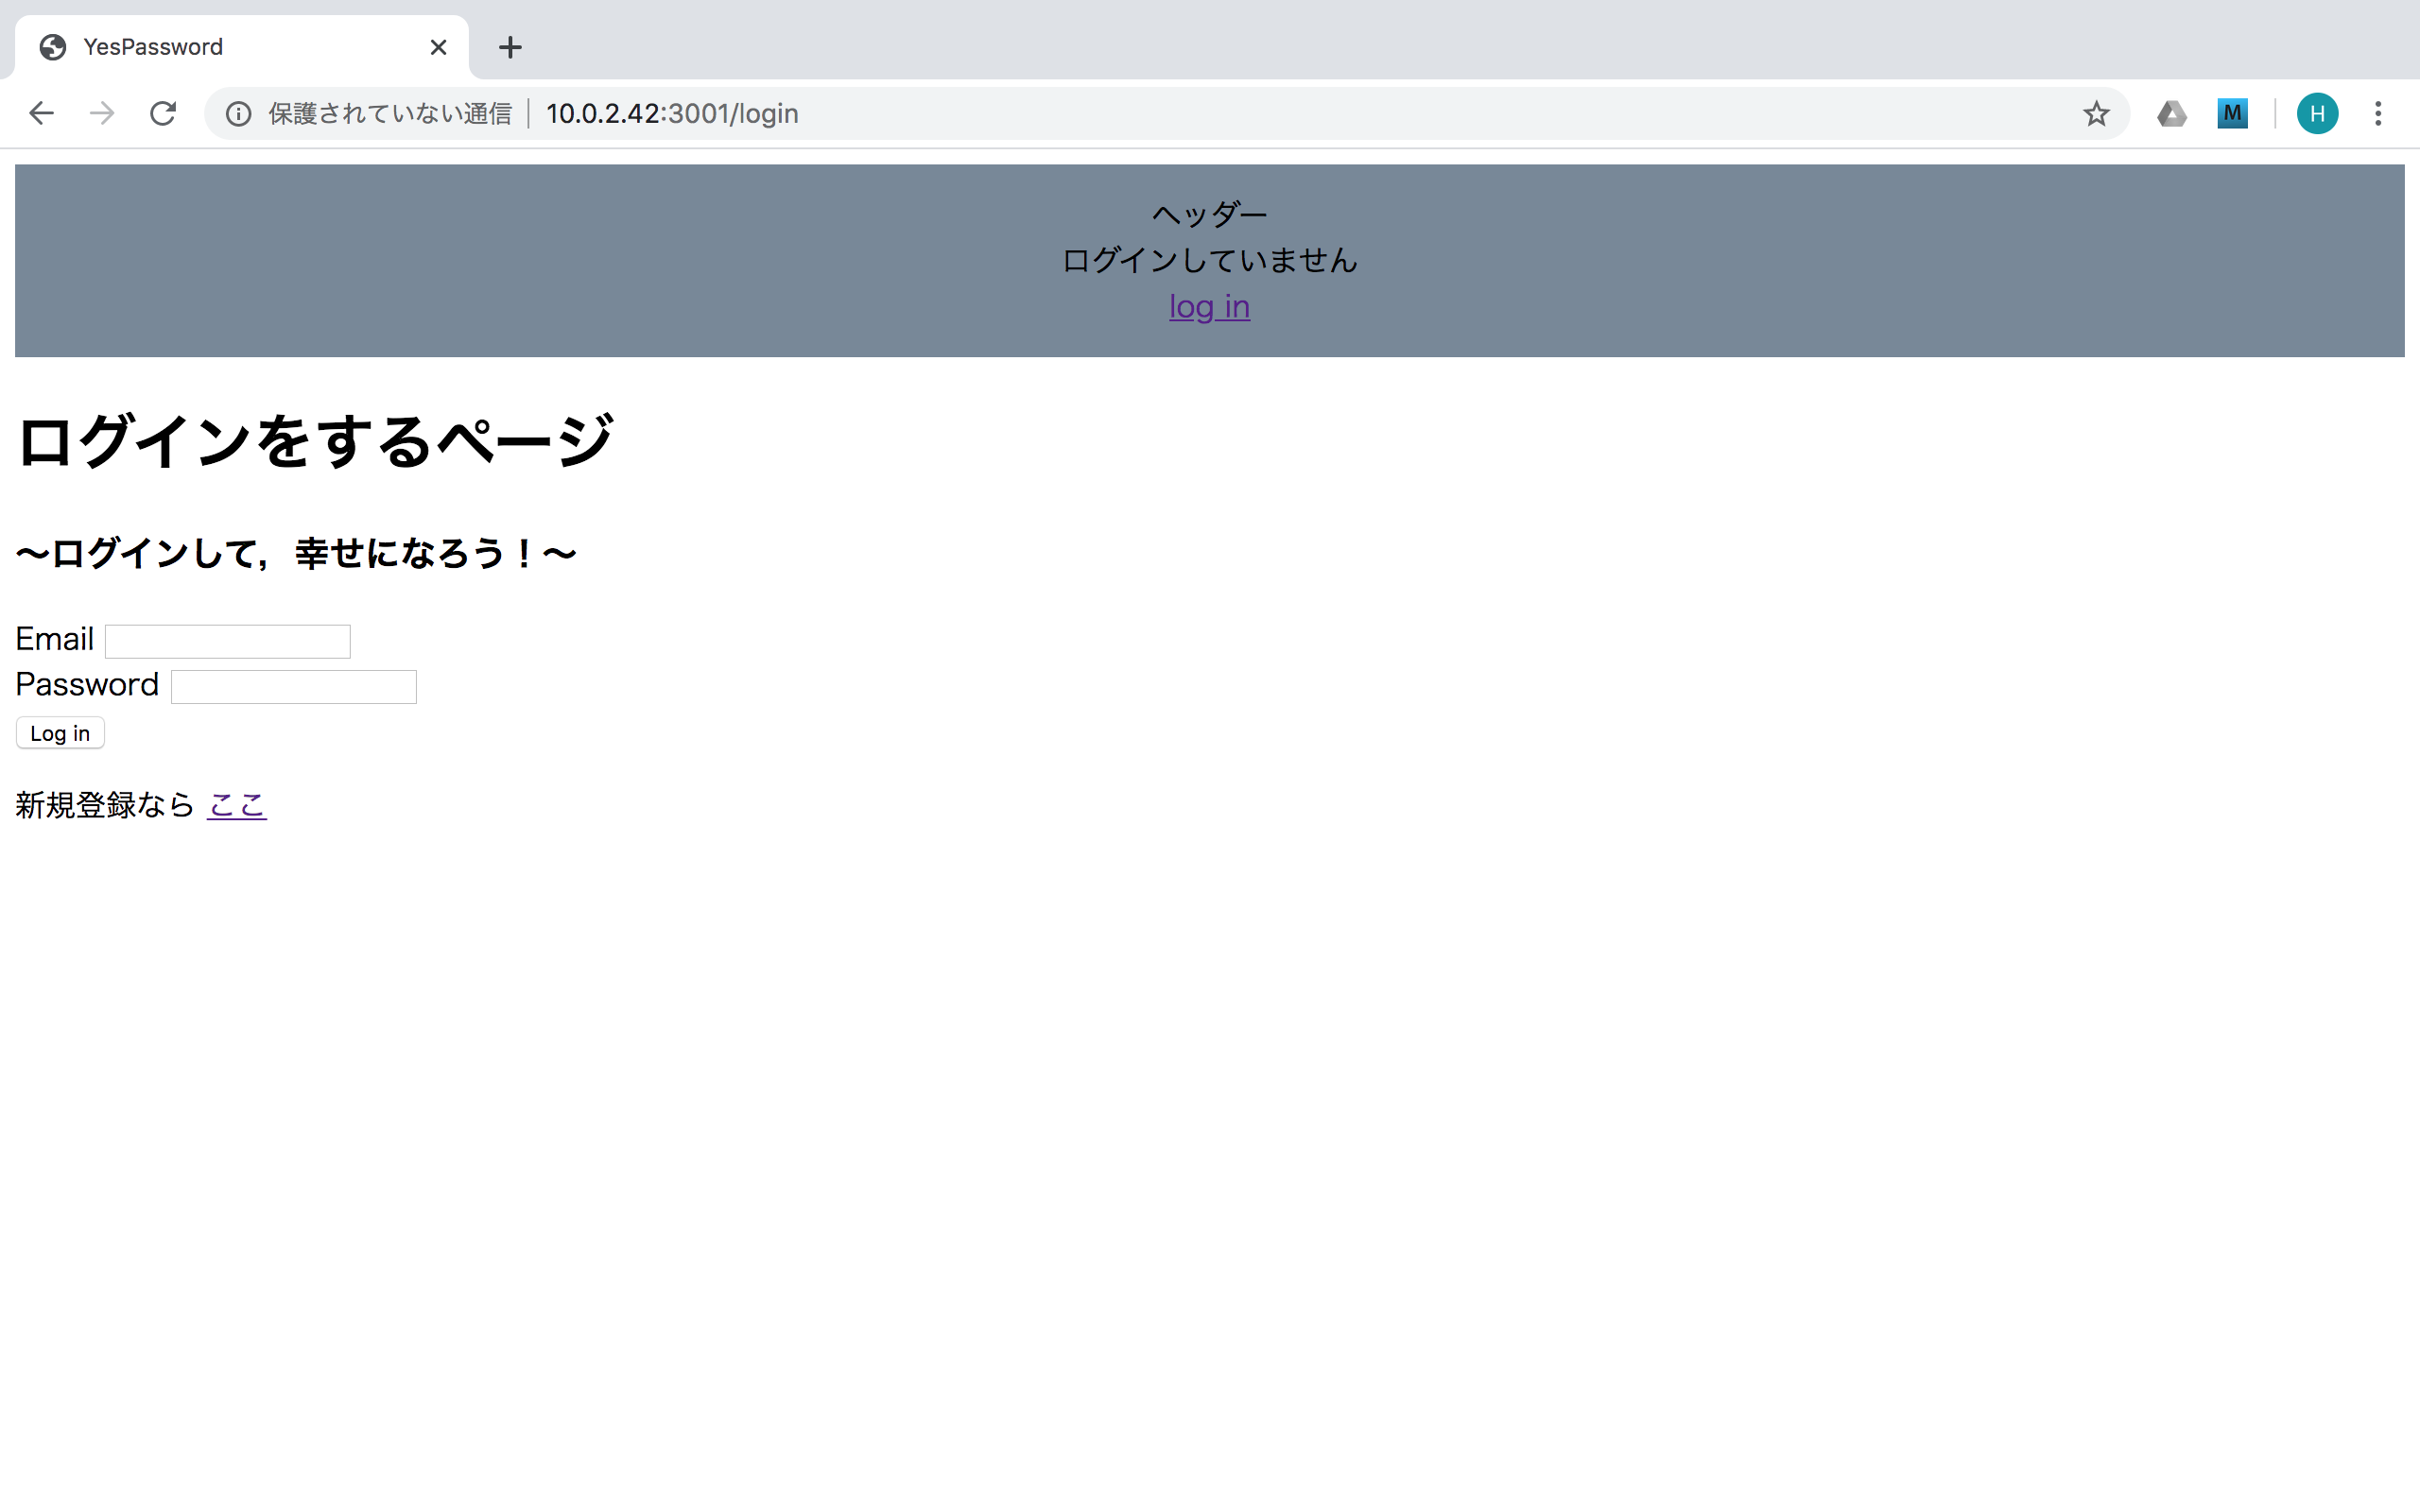
\includegraphics[height=8.4cm]{./fig/chapter4/inspect_2/password_screnn/login.png}
        \caption{検証2\_認証(パスワード方式)}
        \label{検証2認証(パスワード方式)}
    \end{figure}

    \vspace{4cm}%図の位置を正しくする!
    %\begin{figure}[h]
    \begin{figure}[H]
        %\centering
        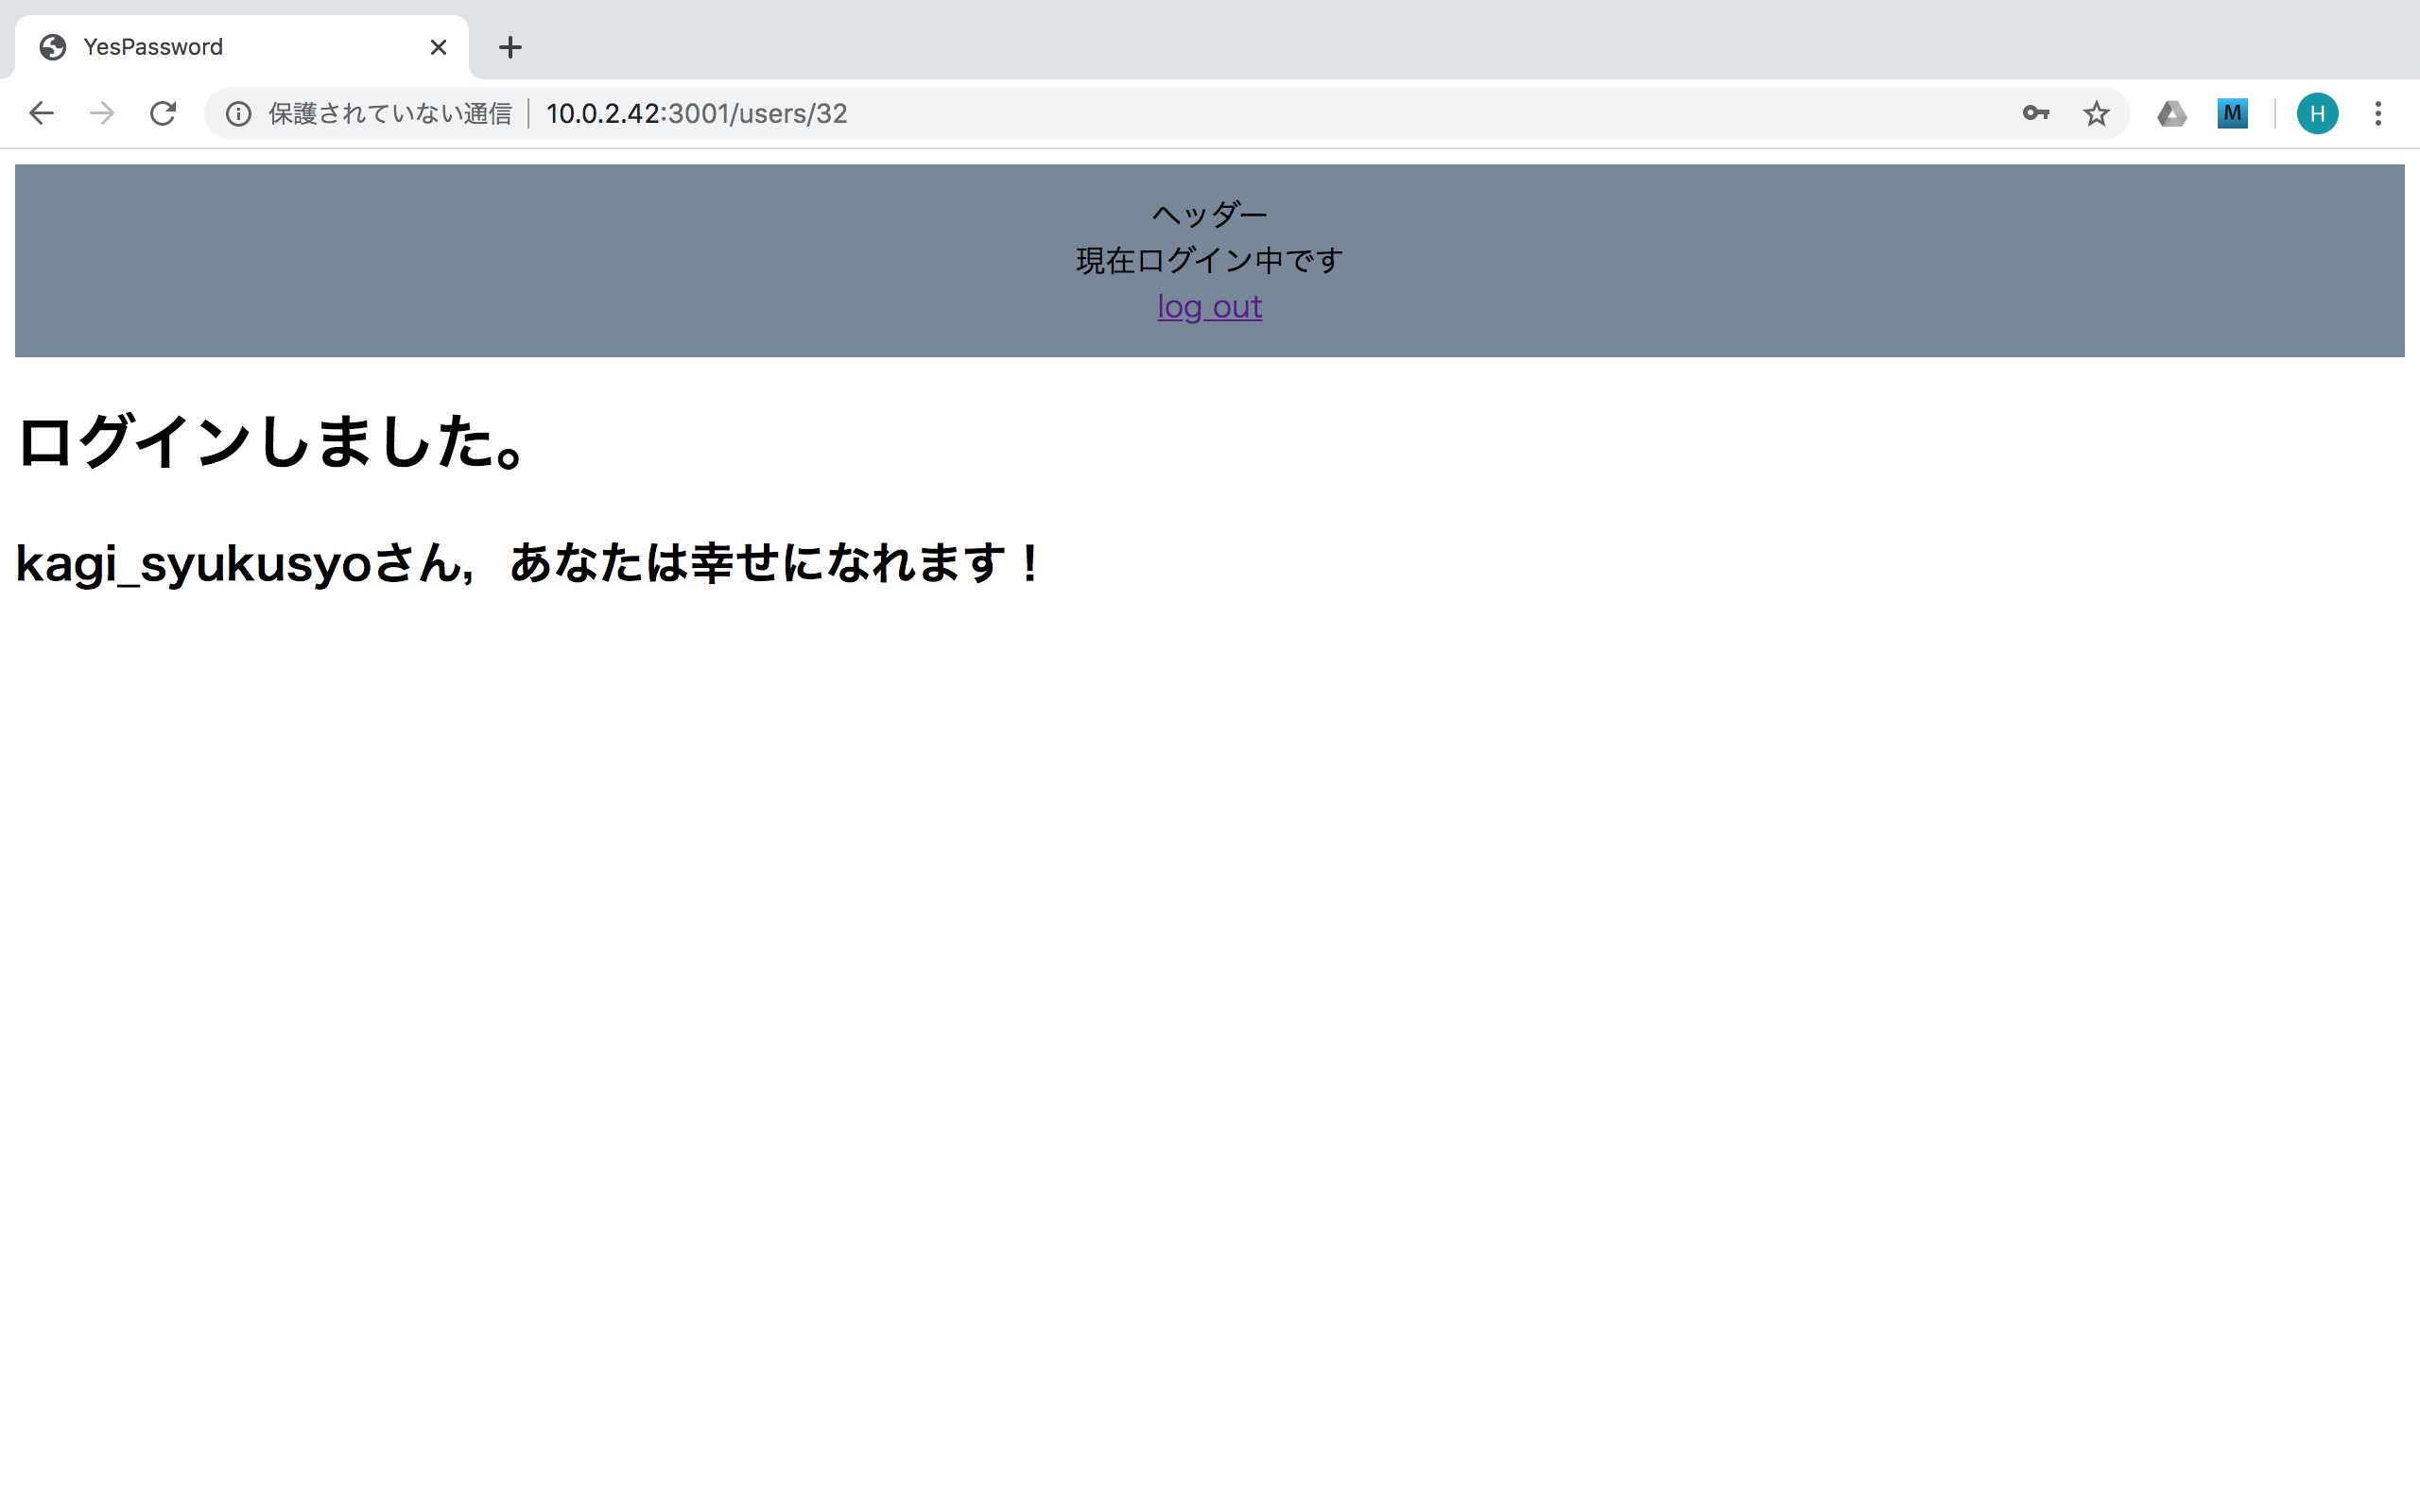
\includegraphics[height=8.4cm]{./fig/chapter4/inspect_2/password_screnn/success.png}
        \caption{検証2\_認証成功後(パスワード方式)}
        \label{検証2認証成功後(パスワード方式)}
    \end{figure}
    % パスワード方式のスクショ---------------------------

    % 鍵方式のスクショ----------------------------------
    \vspace{4cm}%図の位置を正しくする!
    \begin{figure}[H]
        %\centering
        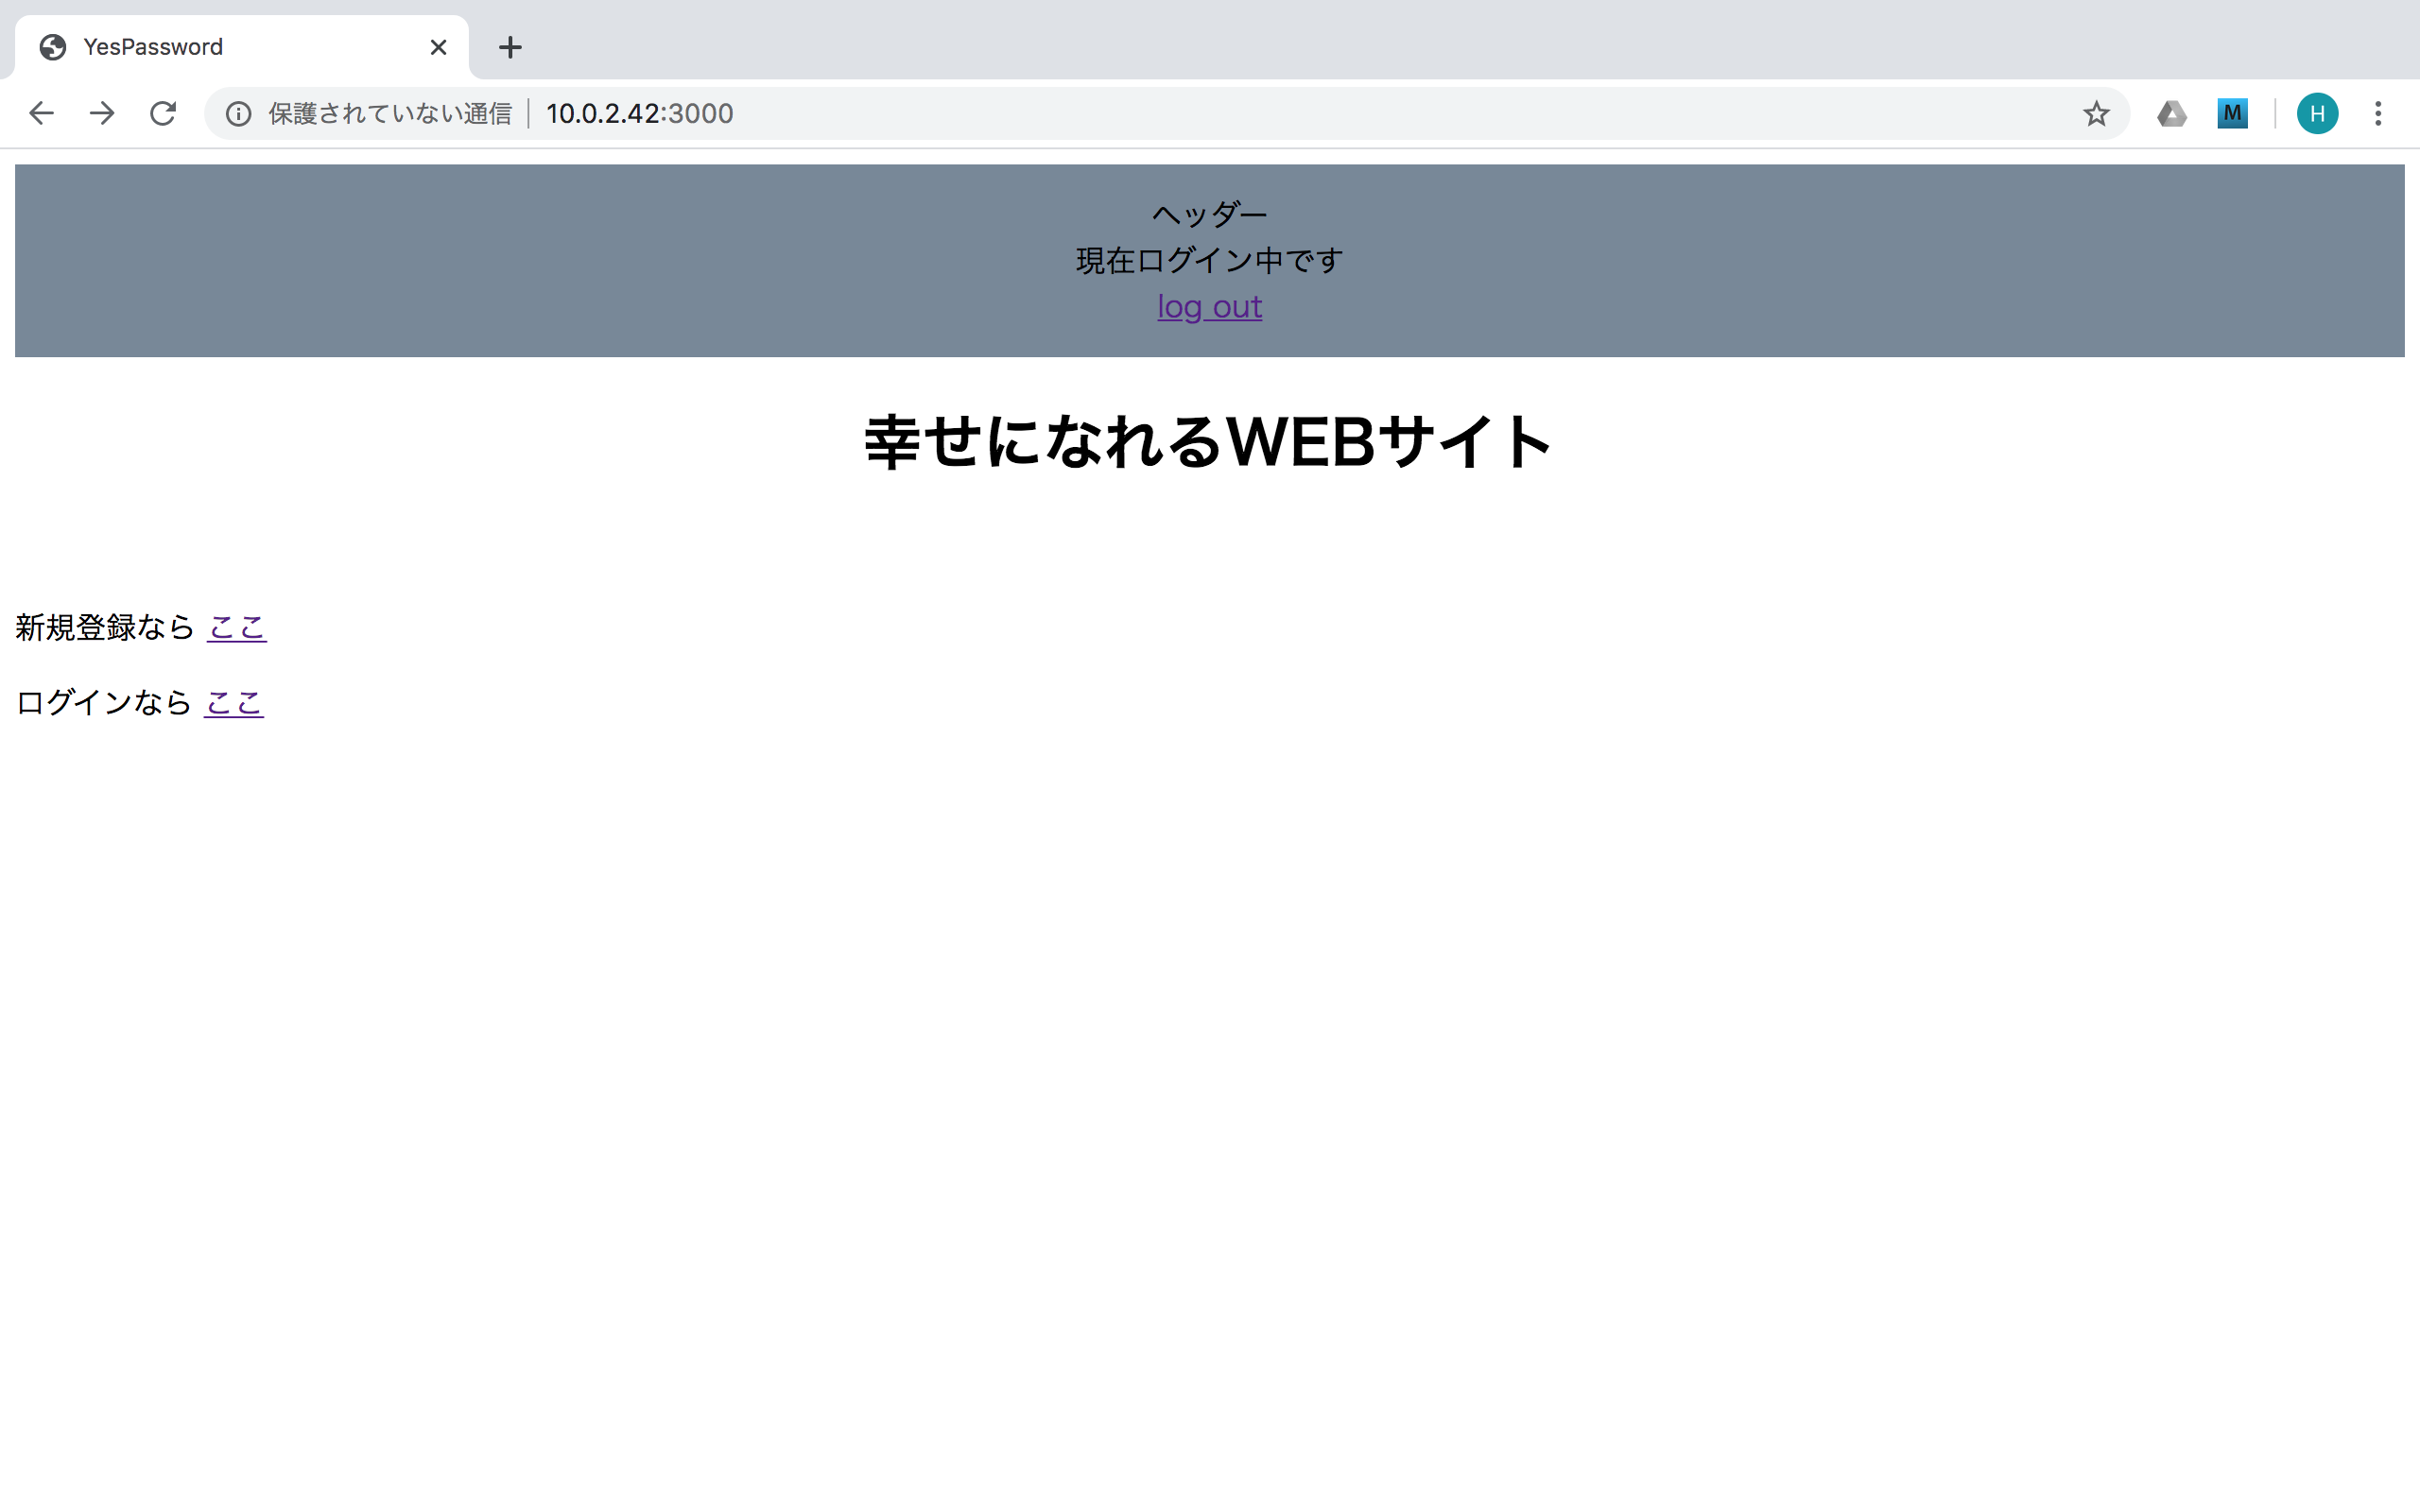
\includegraphics[height=8.4cm]{./fig/chapter4/inspect_2/key_screnn/home.png}
        \caption{検証2\_ホーム画面(鍵方式)}
        \label{検証2ホーム画面(鍵方式)}
    \end{figure}

    \vspace{4cm}%図の位置を正しくする!
    \begin{figure}[H]
        %\centering
        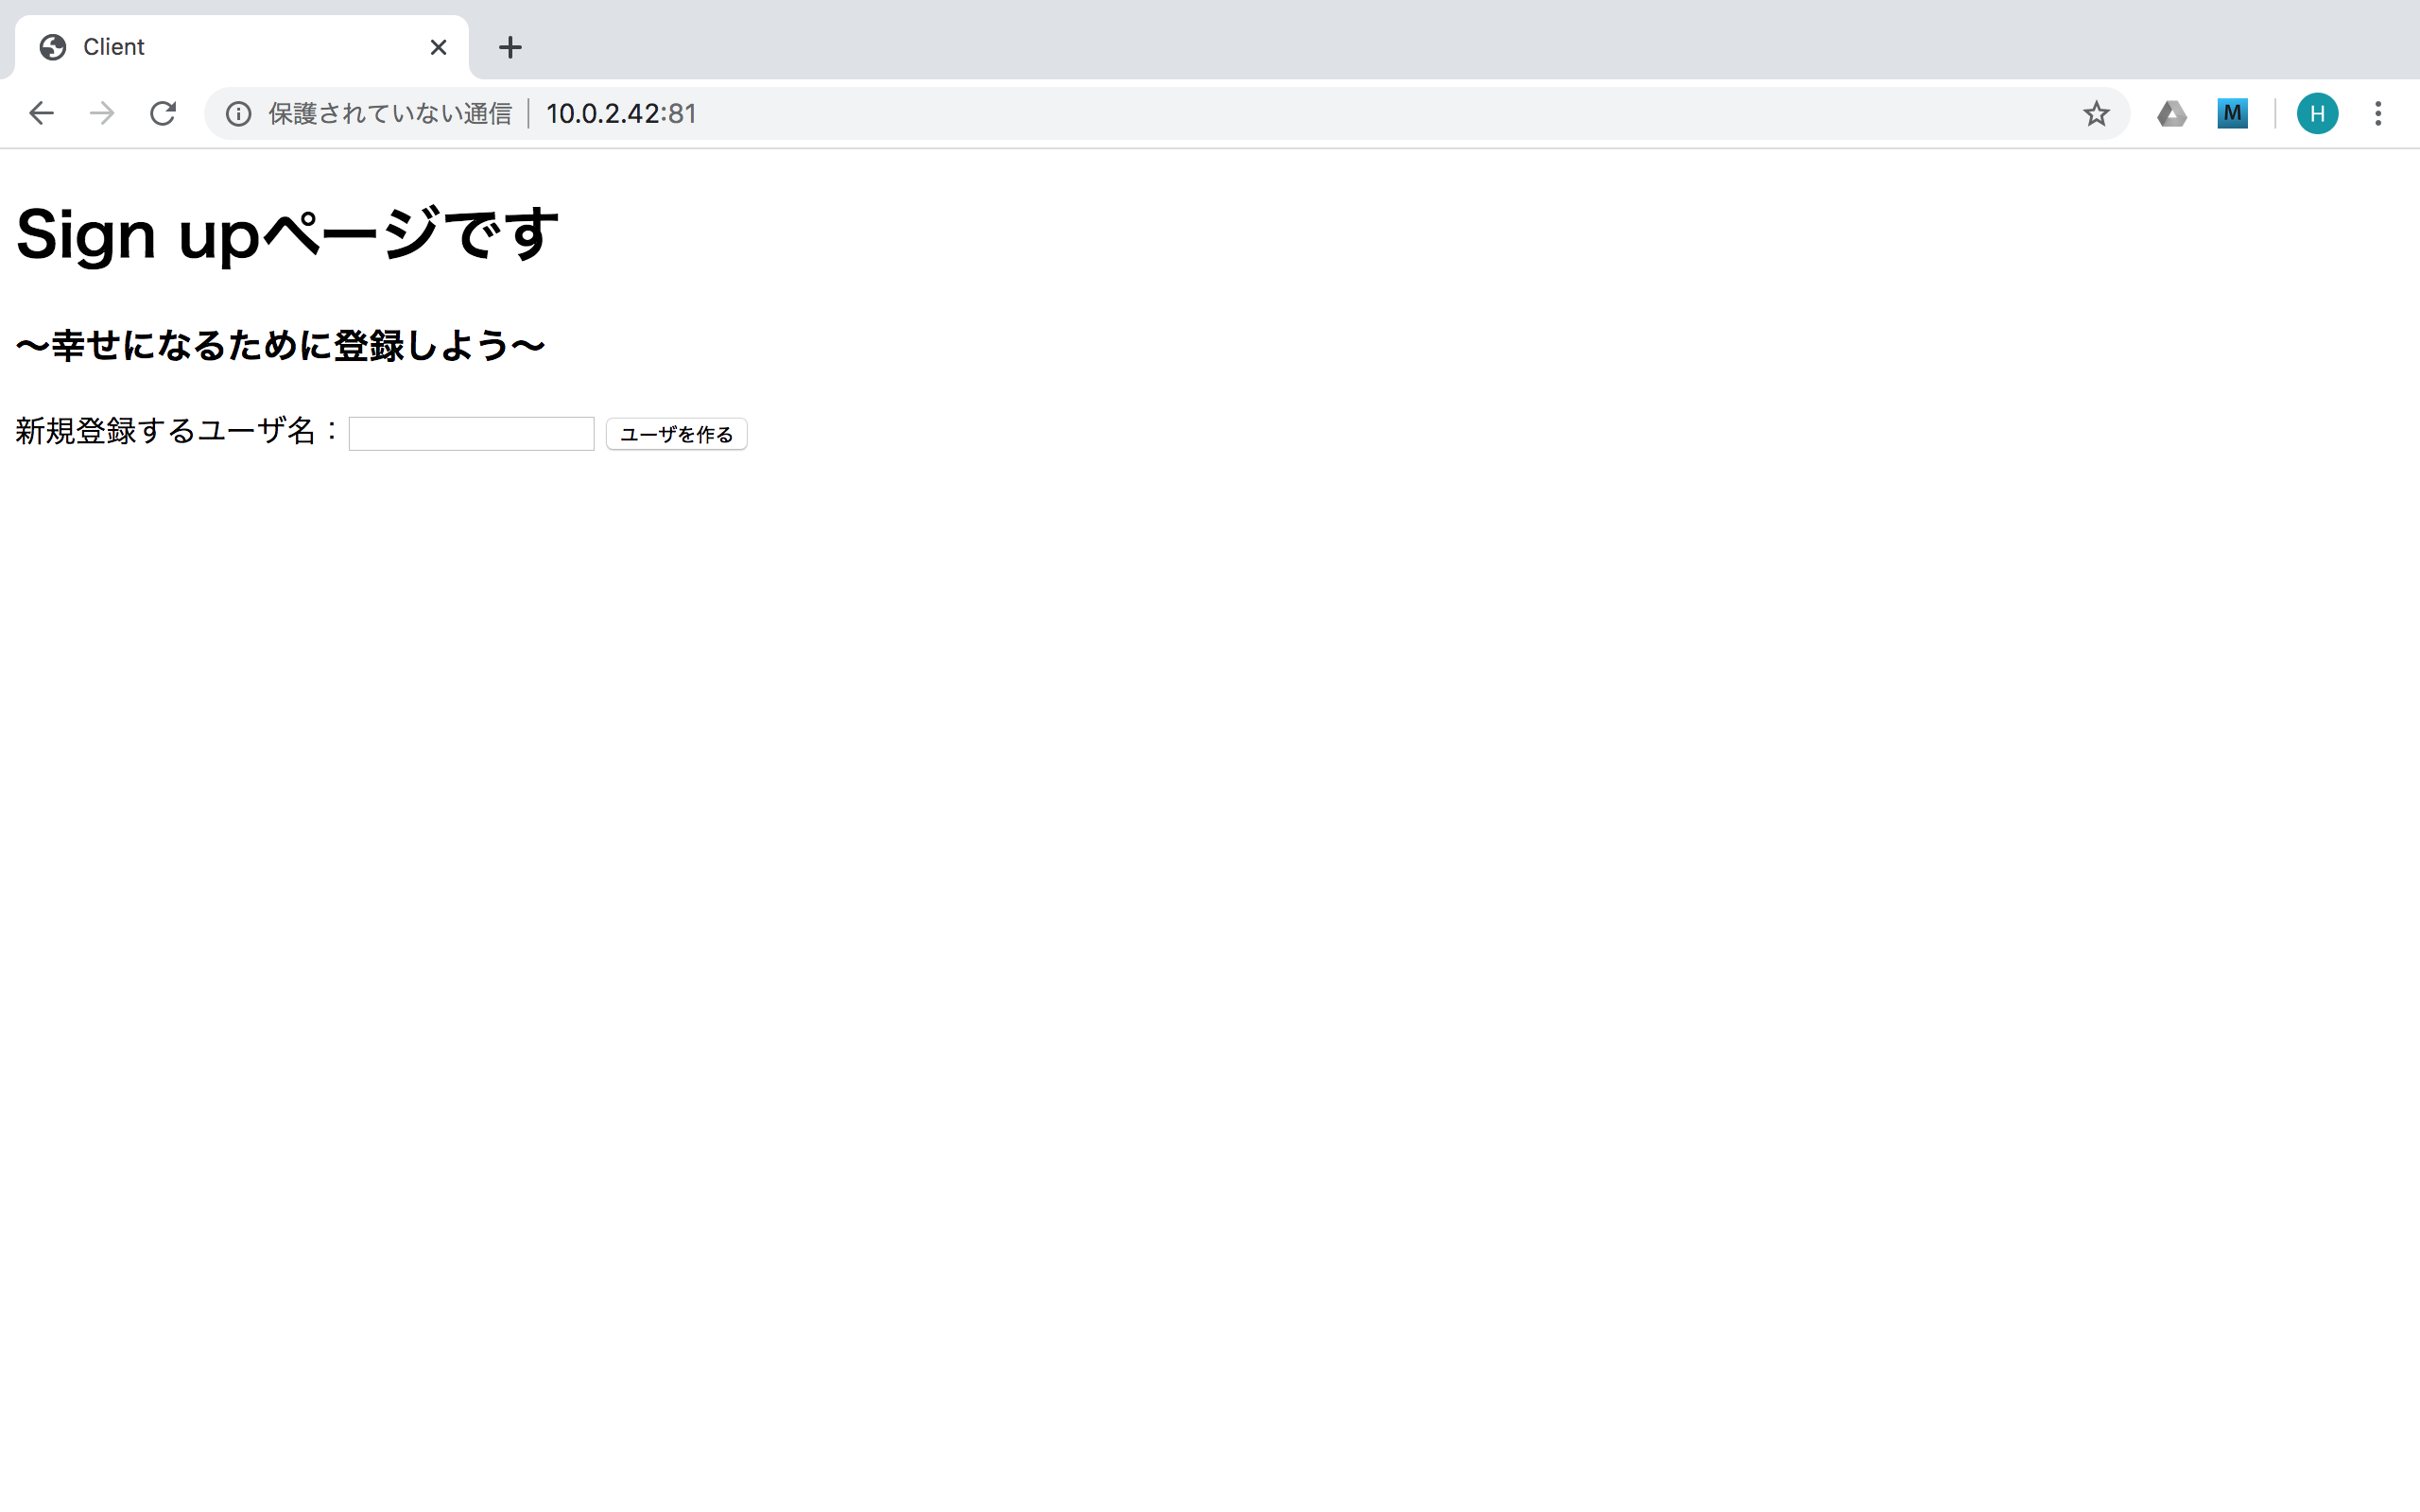
\includegraphics[height=8.4cm]{./fig/chapter4/inspect_2/key_screnn/sign_up.png}
        \caption{検証2\_アカウント作成(鍵方式)}
        \label{検証2アカウント作成(鍵方式)}
    \end{figure}

    \vspace{4cm}%図の位置を正しくする!
    \begin{figure}[H]
        %\centering
        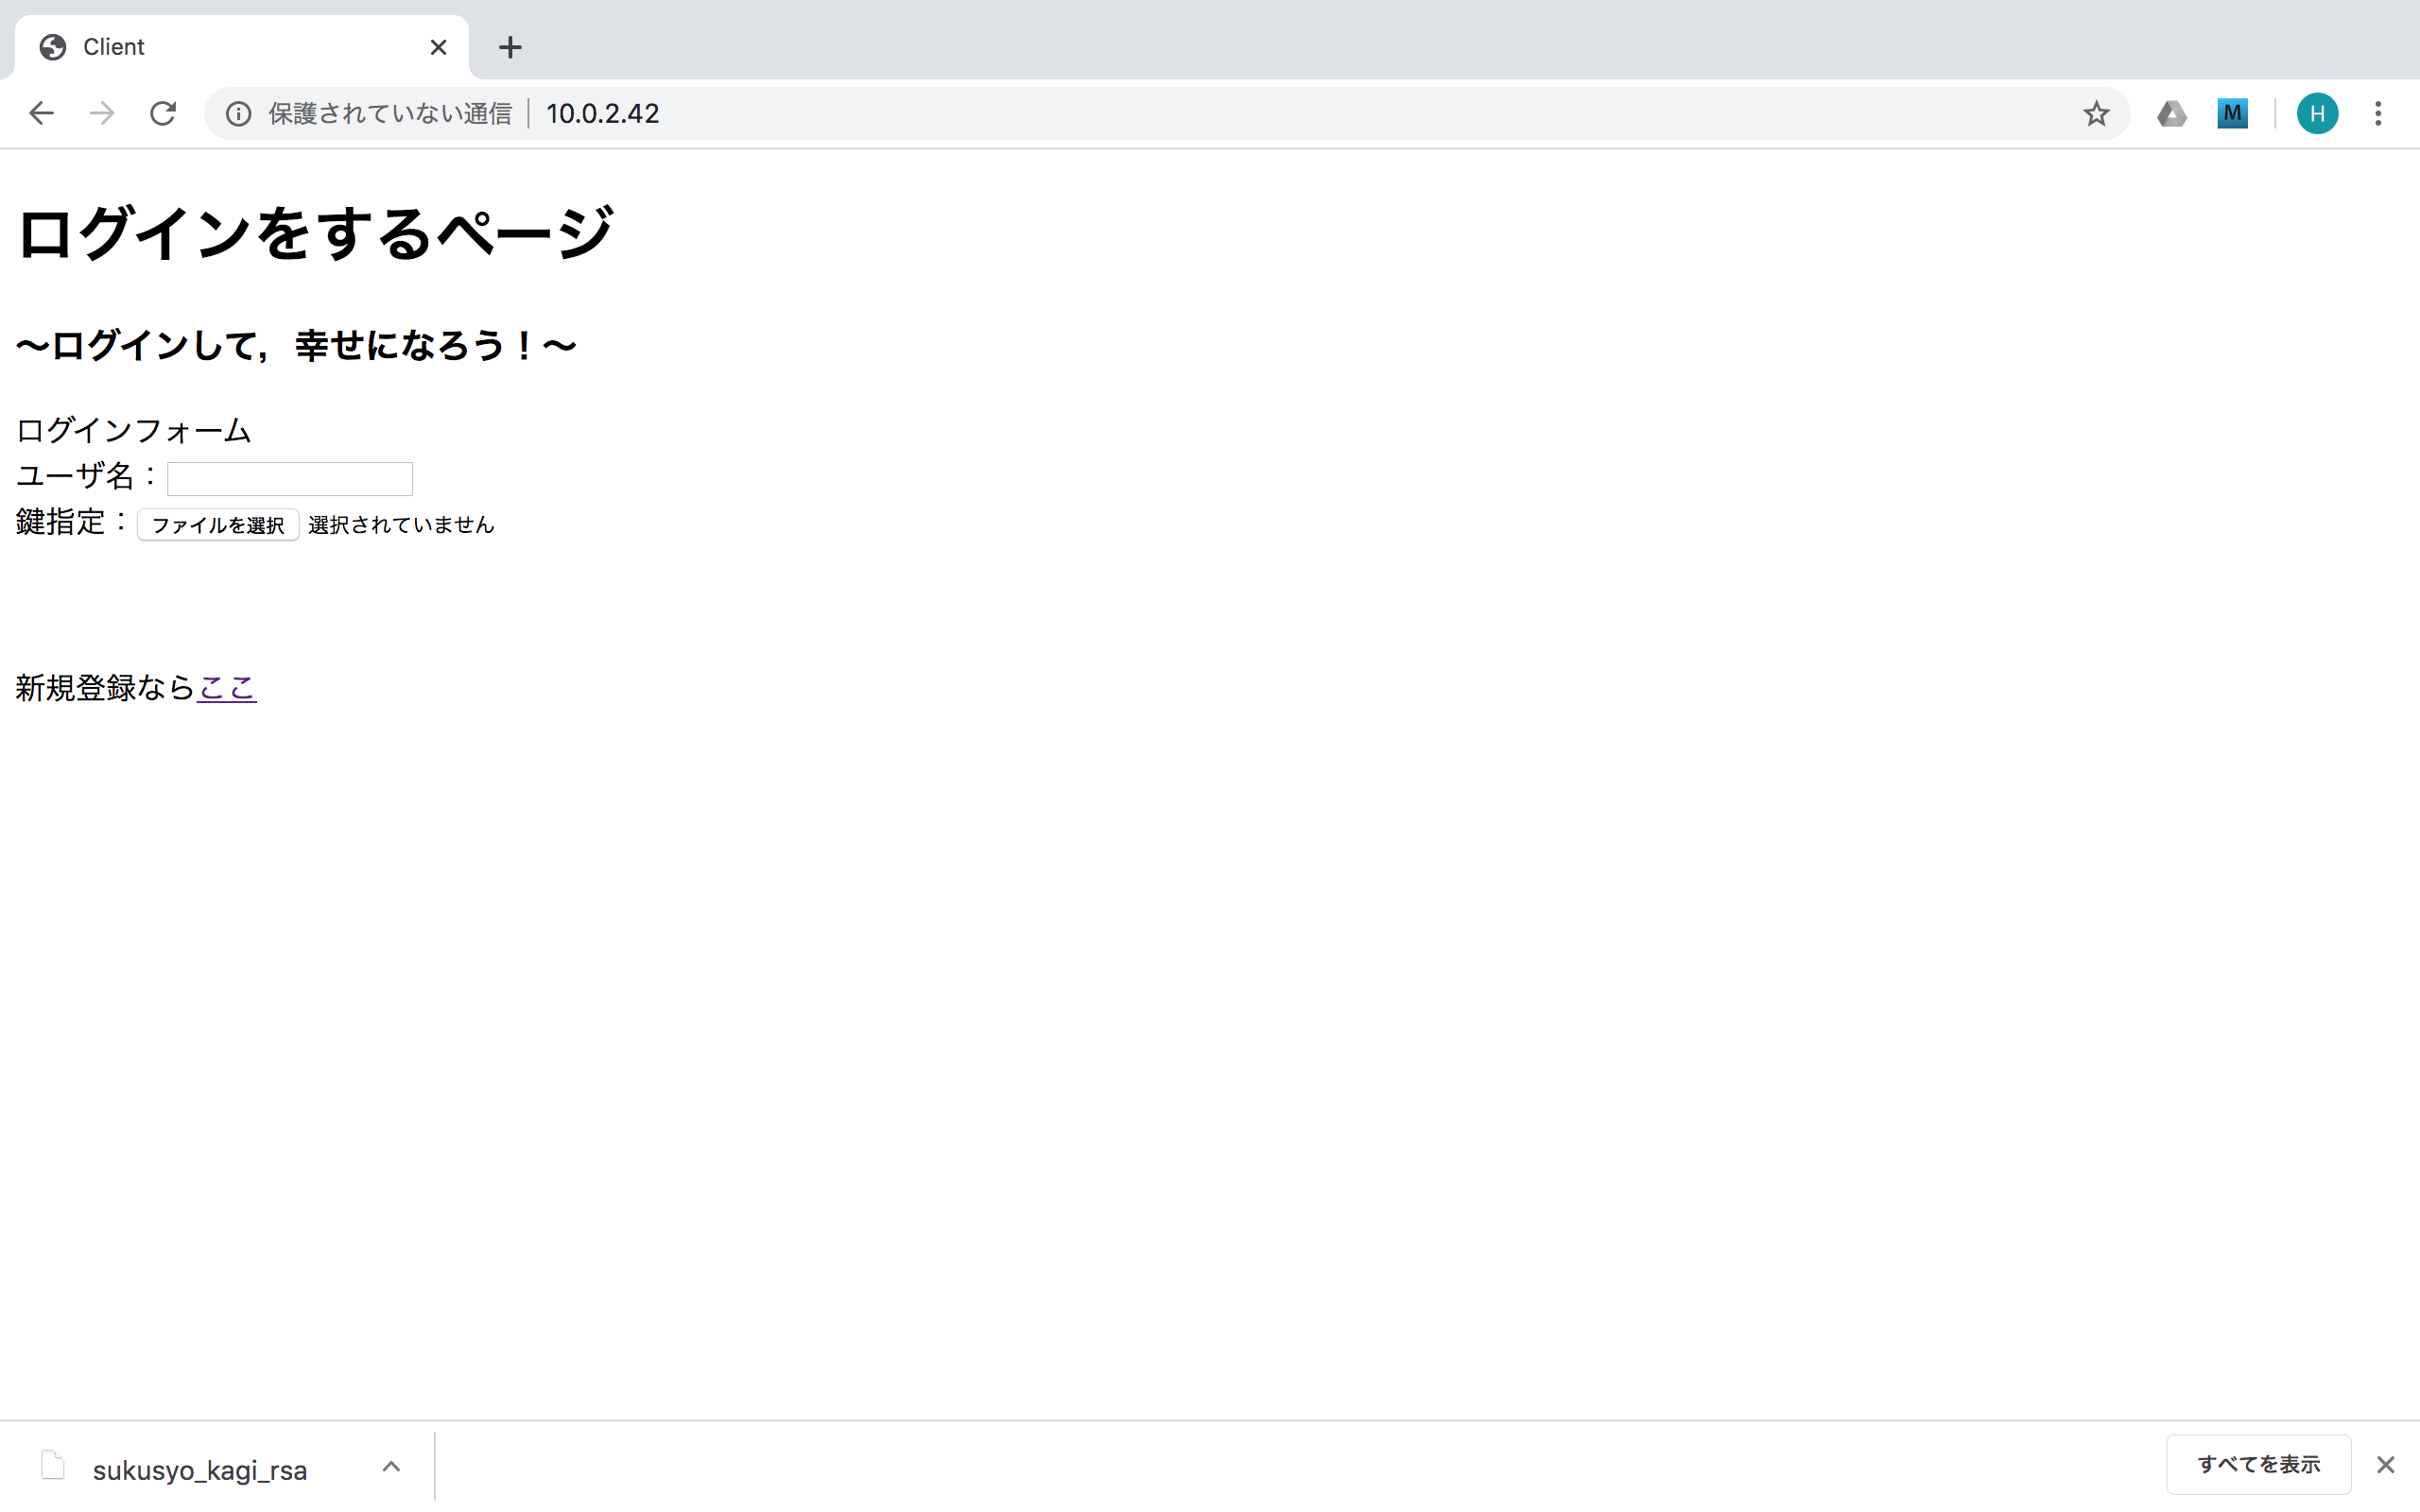
\includegraphics[height=8.4cm]{./fig/chapter4/inspect_2/key_screnn/login.png}
        \caption{検証2\_認証(鍵方式)}
        \label{検証2認証(鍵方式)}
    \end{figure}

    \vspace{4cm}%図の位置を正しくする!
    \begin{figure}[H]
        %\centering
        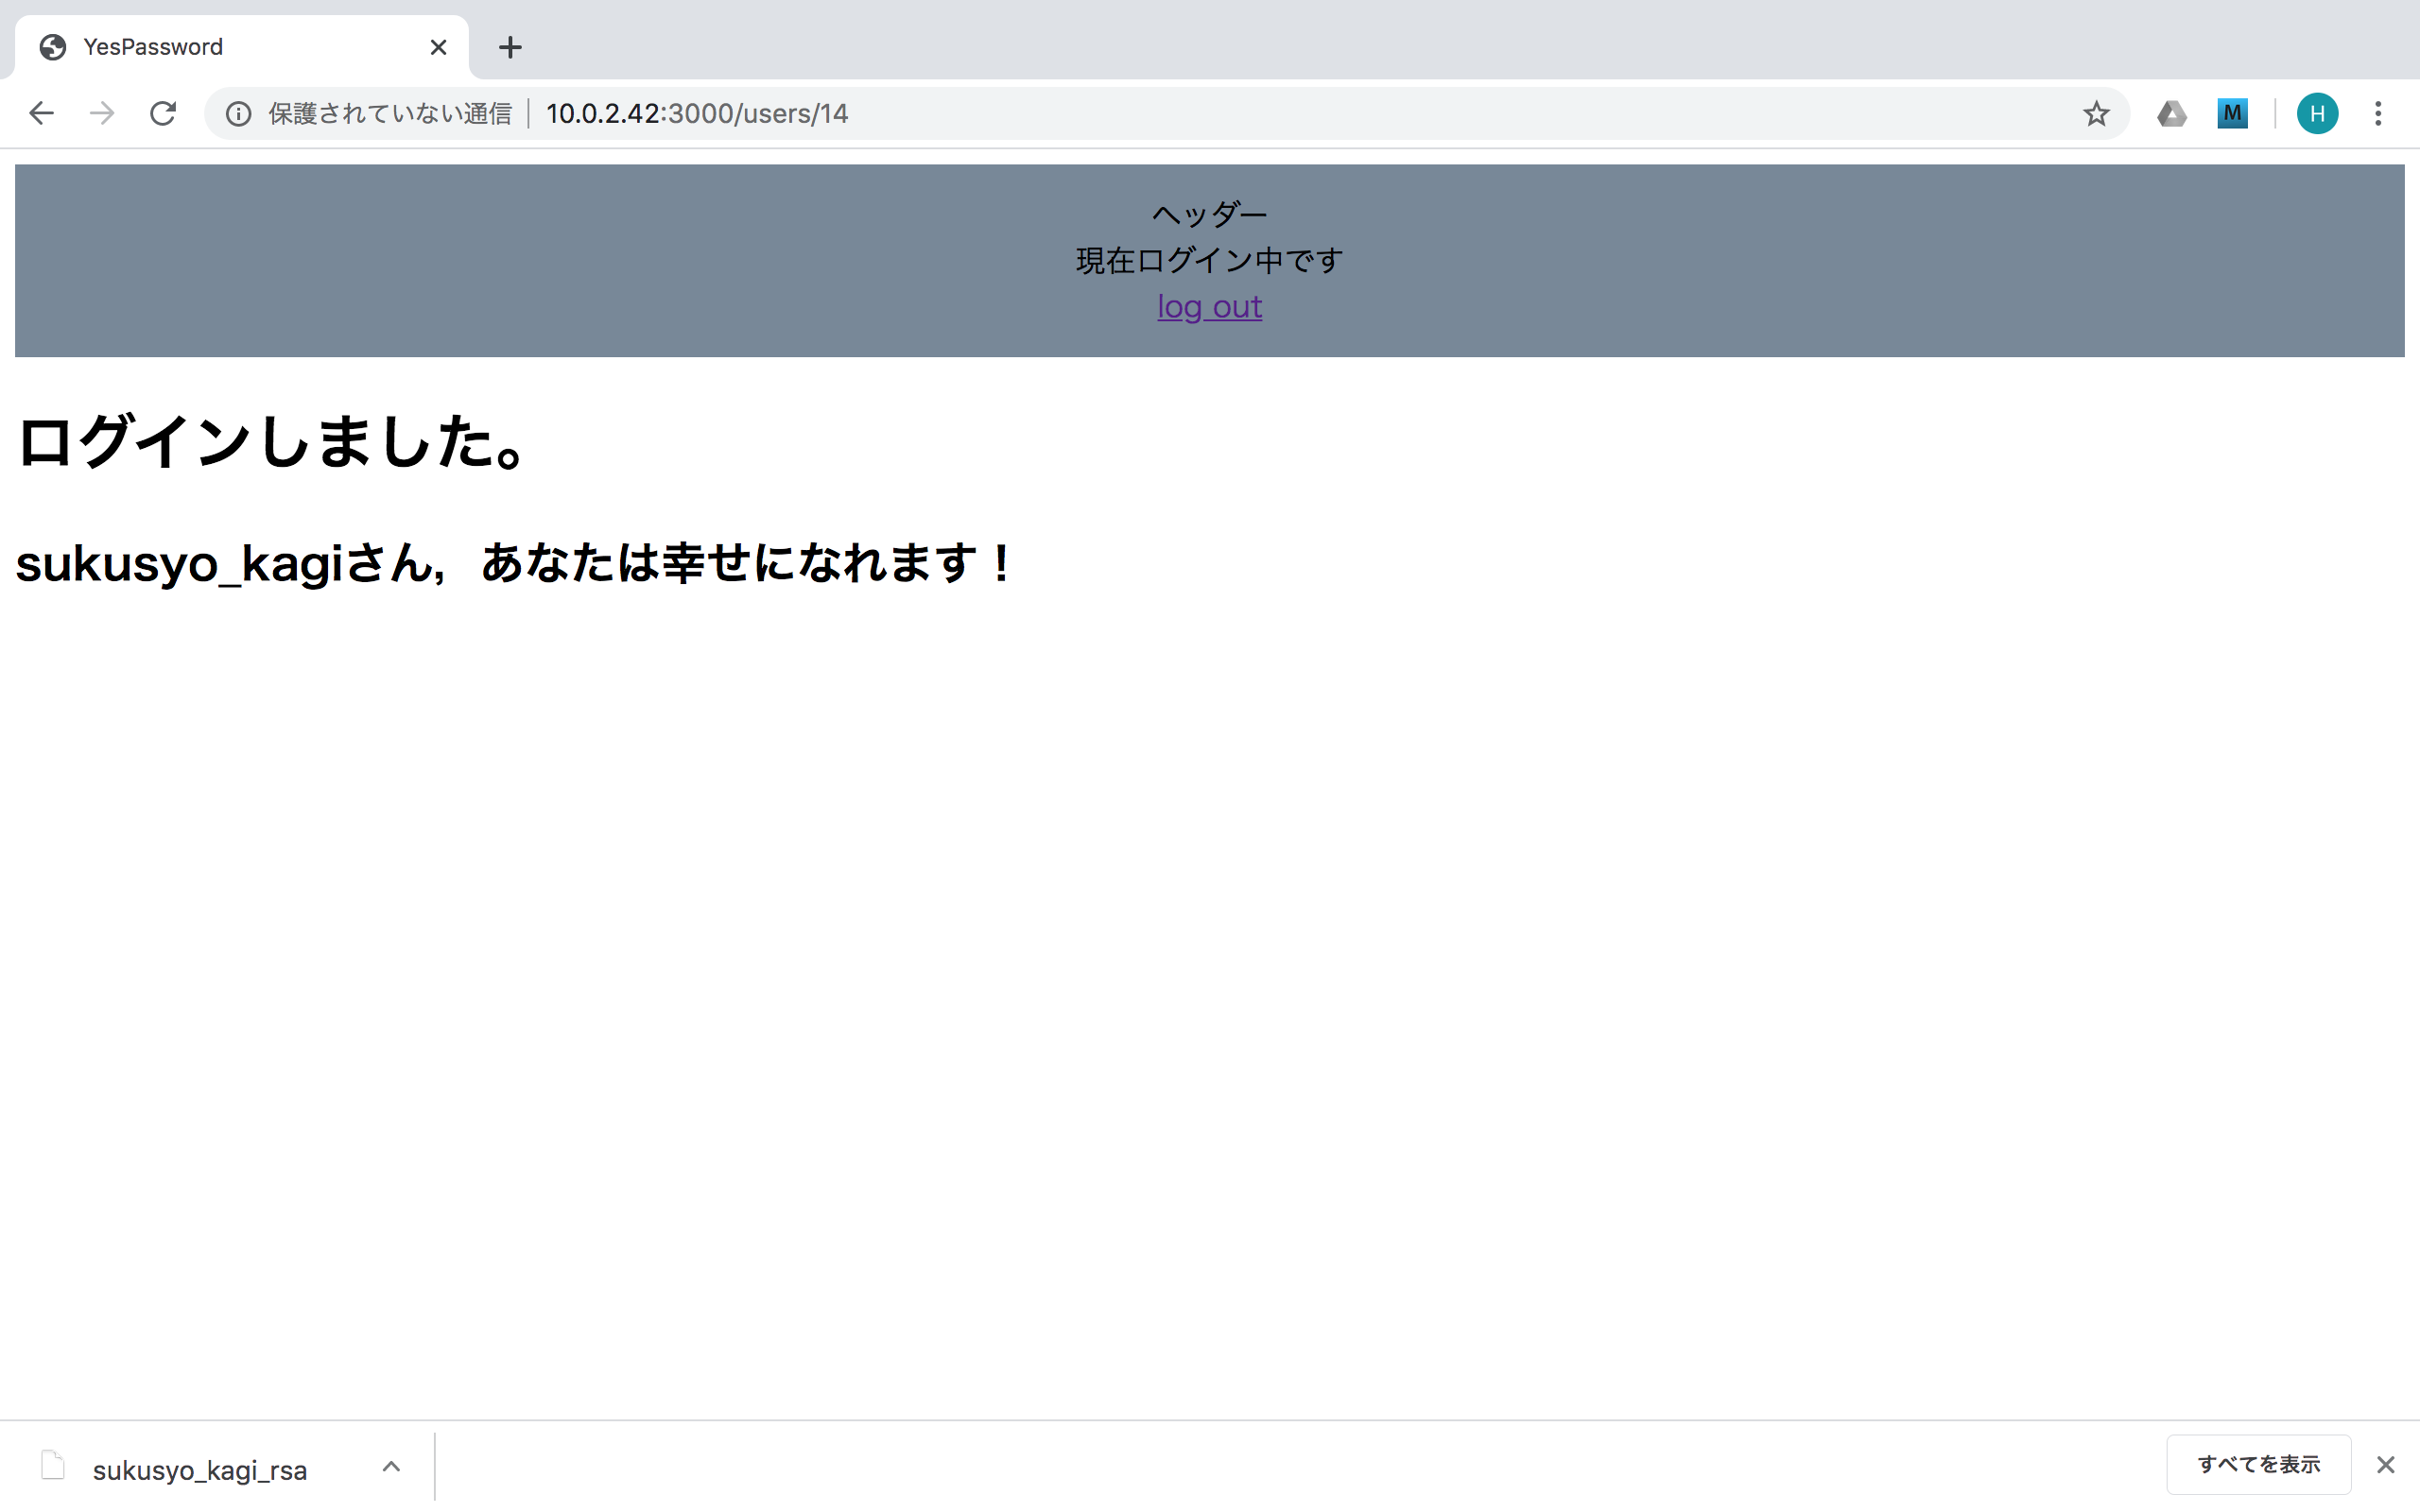
\includegraphics[height=8.4cm]{./fig/chapter4/inspect_2/key_screnn/login-after2.png}
        \caption{検証2\_認証成功後(鍵方式)}
        \label{検証2認証成功後(鍵方式)}
    \end{figure}
    % 鍵方式のスクショ---------------------------------- 

    % アンケートは検証1と同じ質問(意図)をしているため,割愛する。








   
    \newpage


    \subsubsection{検証マニュアル}
    以下の図\ref{検証2マニュアル1},図\ref{検証2マニュアル2},図\ref{検証2マニュアル3}は,上記の図\ref{検証2アカウント作成(パスワード方式)} 〜 図\ref{検証2アカウント作成(鍵方式)} ,図\ref{アンケート1} 〜 図\ref{アンケート4}
    の検証を行うためのマニュアルである.
    マニュアルを作成して,検証を行った意図としては,再現性を持って検証を行うためである.

    次に,検証1のマニュアルと比べての相違点とその意図を以下に述べる.\\
    パスワードの使い回し,password というパスワードなど,日常的に設定しないと思われるパスワードの設定が見受けられた。
    そのため,マニュアル(図\ref{検証2マニュアル1})に 「普段用いるように」,と被験者に注意を促す。
    また,パスワードの設定に関して,日常的に設定ような,より効果的な検証を行うためには,
    アカウントの登録で,パスワードに対して,バリデーション(パスワードの制限)をすることがあげられる。
    しかし,今回の検証では,あえてバリデーションをかけないことにする。
    理由は,
        鍵認証方式の,セキュリティは脆弱性が大きいのに対して,
        パスワード方式のだけセキュアにすると,検証比較として適していないと判断したためである。

    %何をやっているのかわからない
    鍵方式での,登録・認証に関して「何やっているかわからない」という意見があった。
    よって,マニュアル(図\ref{検証2マニュアル1},図\ref{検証2マニュアル2})に,「"パスワード方式です" "鍵方式です"」と軽く説明を加える。
    また,鍵方式の登録・認証に対しての,説明を詳しくすると,
    一般的に普及している,パスワード方式 による,被験者の慣れ を検証に含めることができないので,
    軽く「"パスワード方式です" "鍵方式です"」という説明を加えることにする。

    % 言いたいやつ----------------------------------------------------------------------------------------------
    %% マニュアル面(被験者生の動作や生の声から)----------------------------

    %%% より,日常的な検証結果を得るために(パスワード設定)
    %%%%パスワードの使い回し,password というパスワードなど,日常的に設定しないと思われるパスワードの設定が見受けられた。
    %%%%そのため,マニュアル(図????)に 「普段用いるように」,と被験者に注意を促す。
    %%%%また,パスワードの設定に関して,日常的に設定ような,より効果的な検証を行うためには,
    %%%%アカウントの登録で,パスワードに対して,バリデーション(パスワードの制限)をすることがあげられる。
    %%%%しかし,今回の検証では,あえてバリデーションをかけないことにする。
    %%%%理由は,
    %%%%    鍵認証方式の,セキュリティは脆弱性が大きいのに対して,
    %%%%    パスワード方式のだけセキュアにすると,検証比較として適していないと判断したためである。

    %%% 何をやっているのかわからない
    %%%% 鍵方式での,登録・認証に関して「何やっているかわからない」という意見があった。
    %%%% よって,マニュアル(図????)に,「"パスワード方式です" "鍵方式です"」と軽く説明を加える。
    %%%% 鍵方式の登録・認証に対しての,説明を詳しくすると,
    %%%%    一般的に普及している,パスワード方式 による,被験者の慣れ を検証に含めることができないので,
    %%%% 軽く「"パスワード方式です" "鍵方式です"」という説明を加える。
    %% マニュアル面(被験者生の動作や生の声から)----------------------------

    % 言いたいやつ----------------------------------------------------------------------------------------------


    \newpage
    \vspace{4cm}%図の位置を正しくする!
    \begin{figure}[H]
        %\centering
        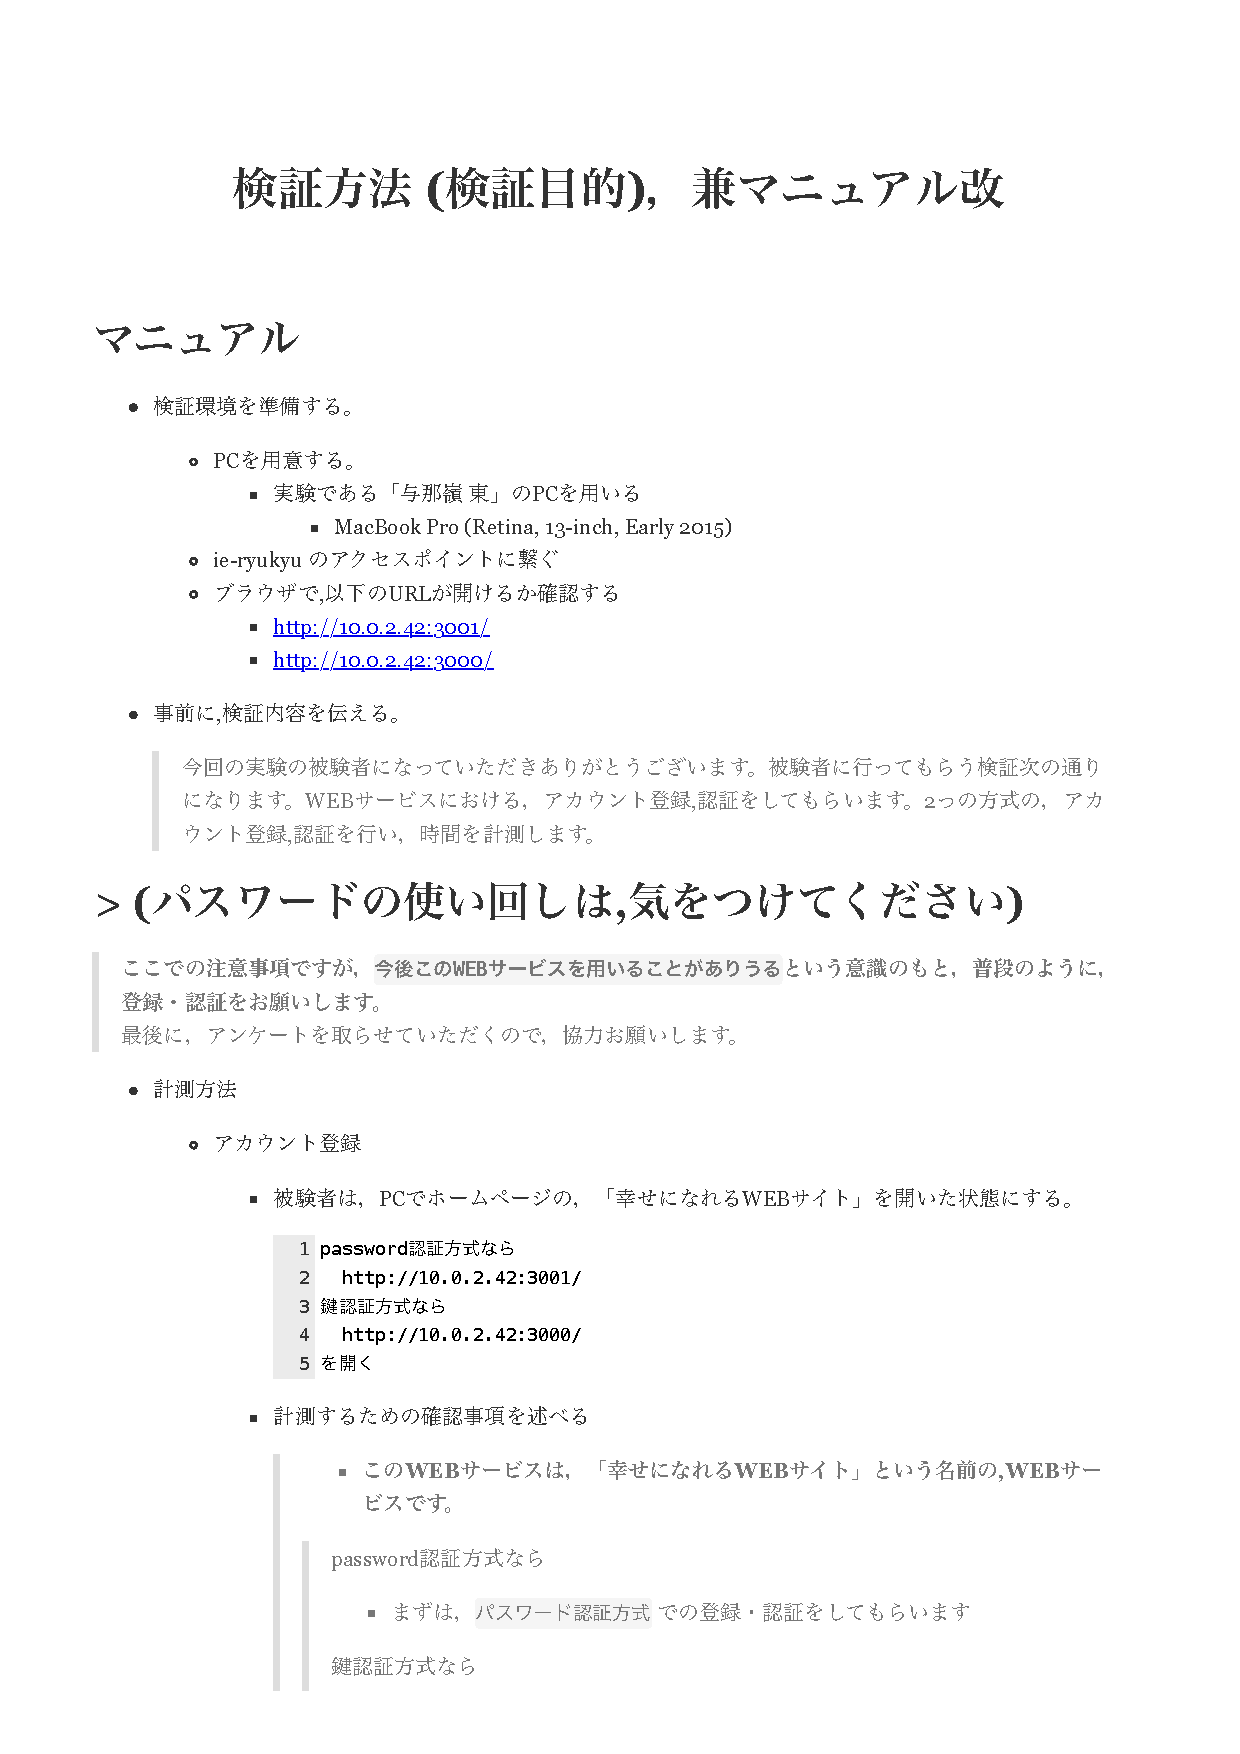
\includegraphics[width=15cm]{./fig/chapter4/inspect_2/manual/manual_1.pdf}
        \caption{検証2マニュアル1}
        \label{検証2マニュアル1}
    \end{figure}

    \vspace{4cm}%図の位置を正しくする!
    \begin{figure}[H]
        %\centering
        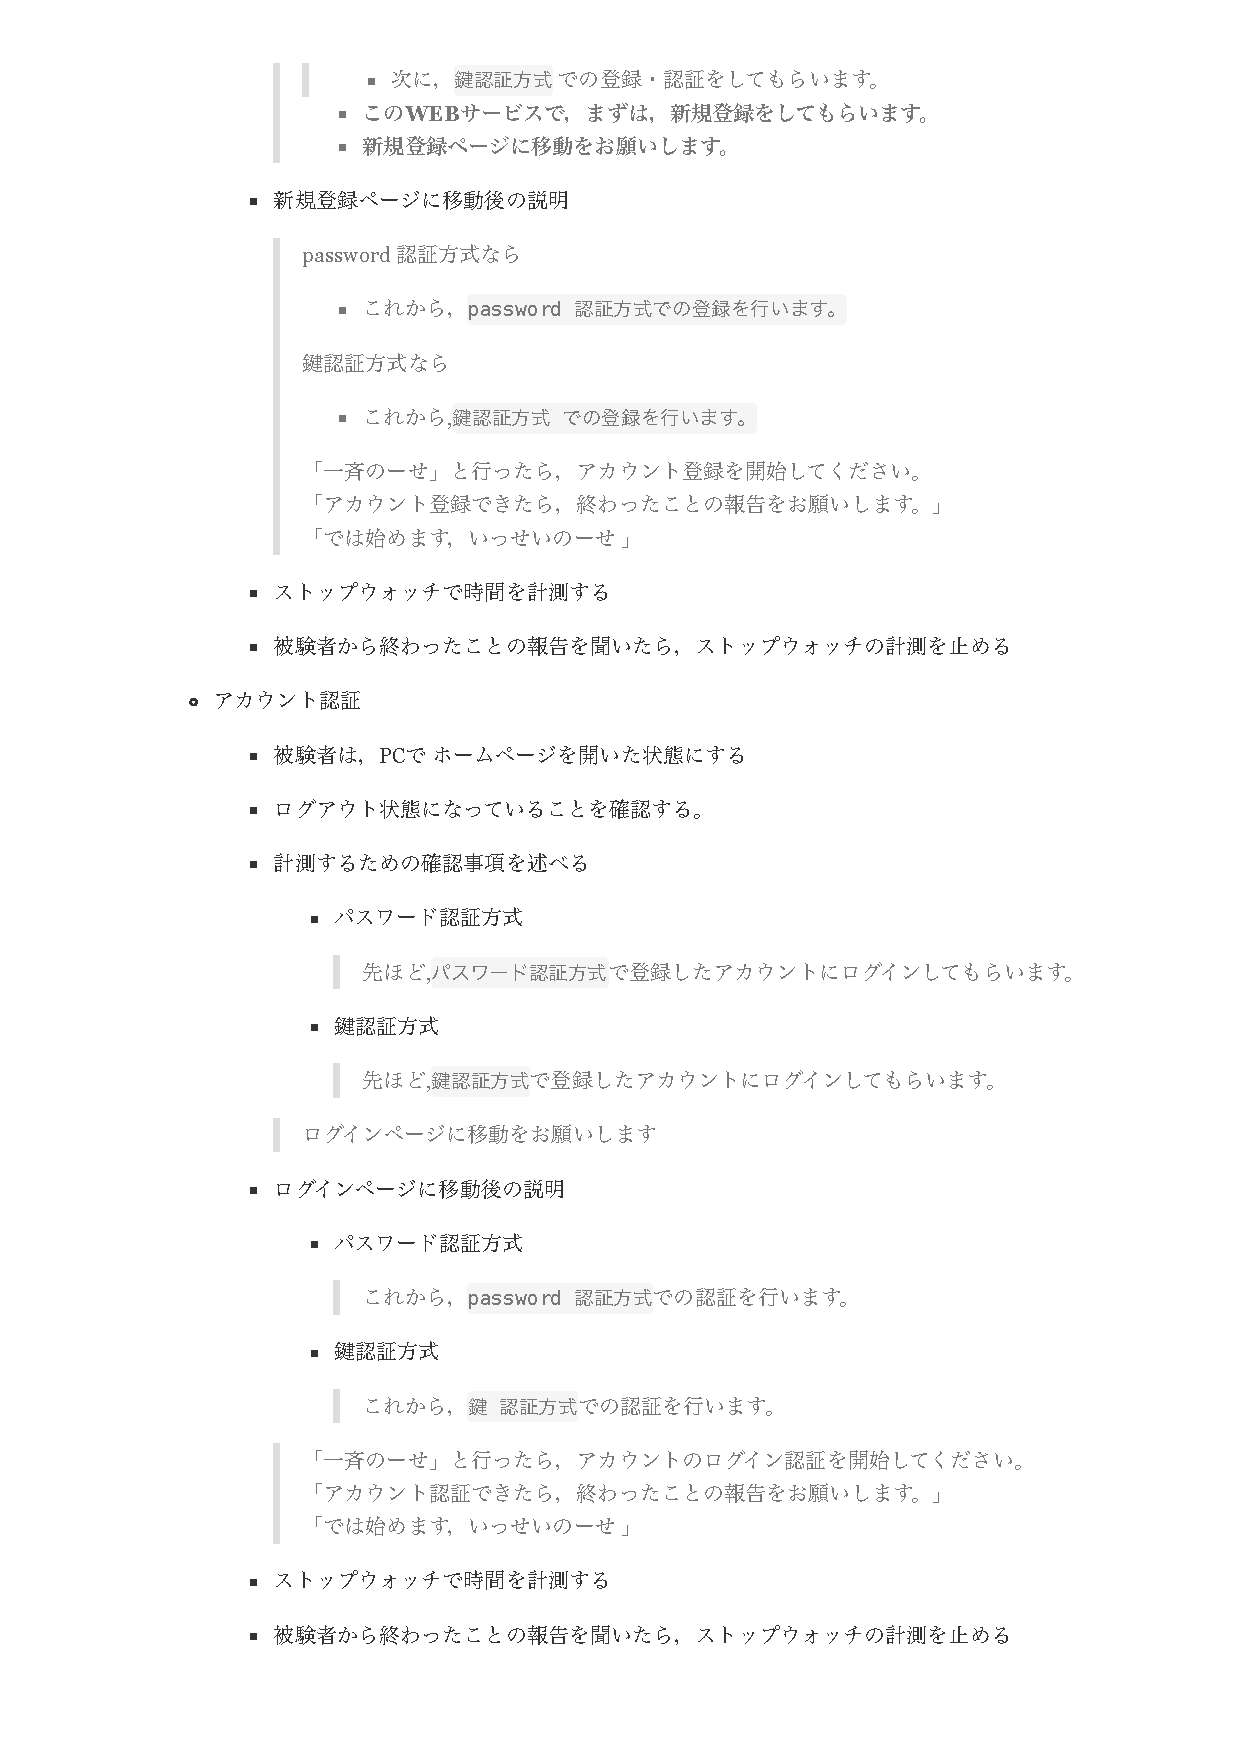
\includegraphics[width=15cm]{./fig/chapter4/inspect_2/manual/manual_2.pdf}
        \caption{検証2マニュアル2}
        \label{検証2マニュアル2}
    \end{figure}

    \vspace{4cm}%図の位置を正しくする!
    \begin{figure}[H]
        %\centering
        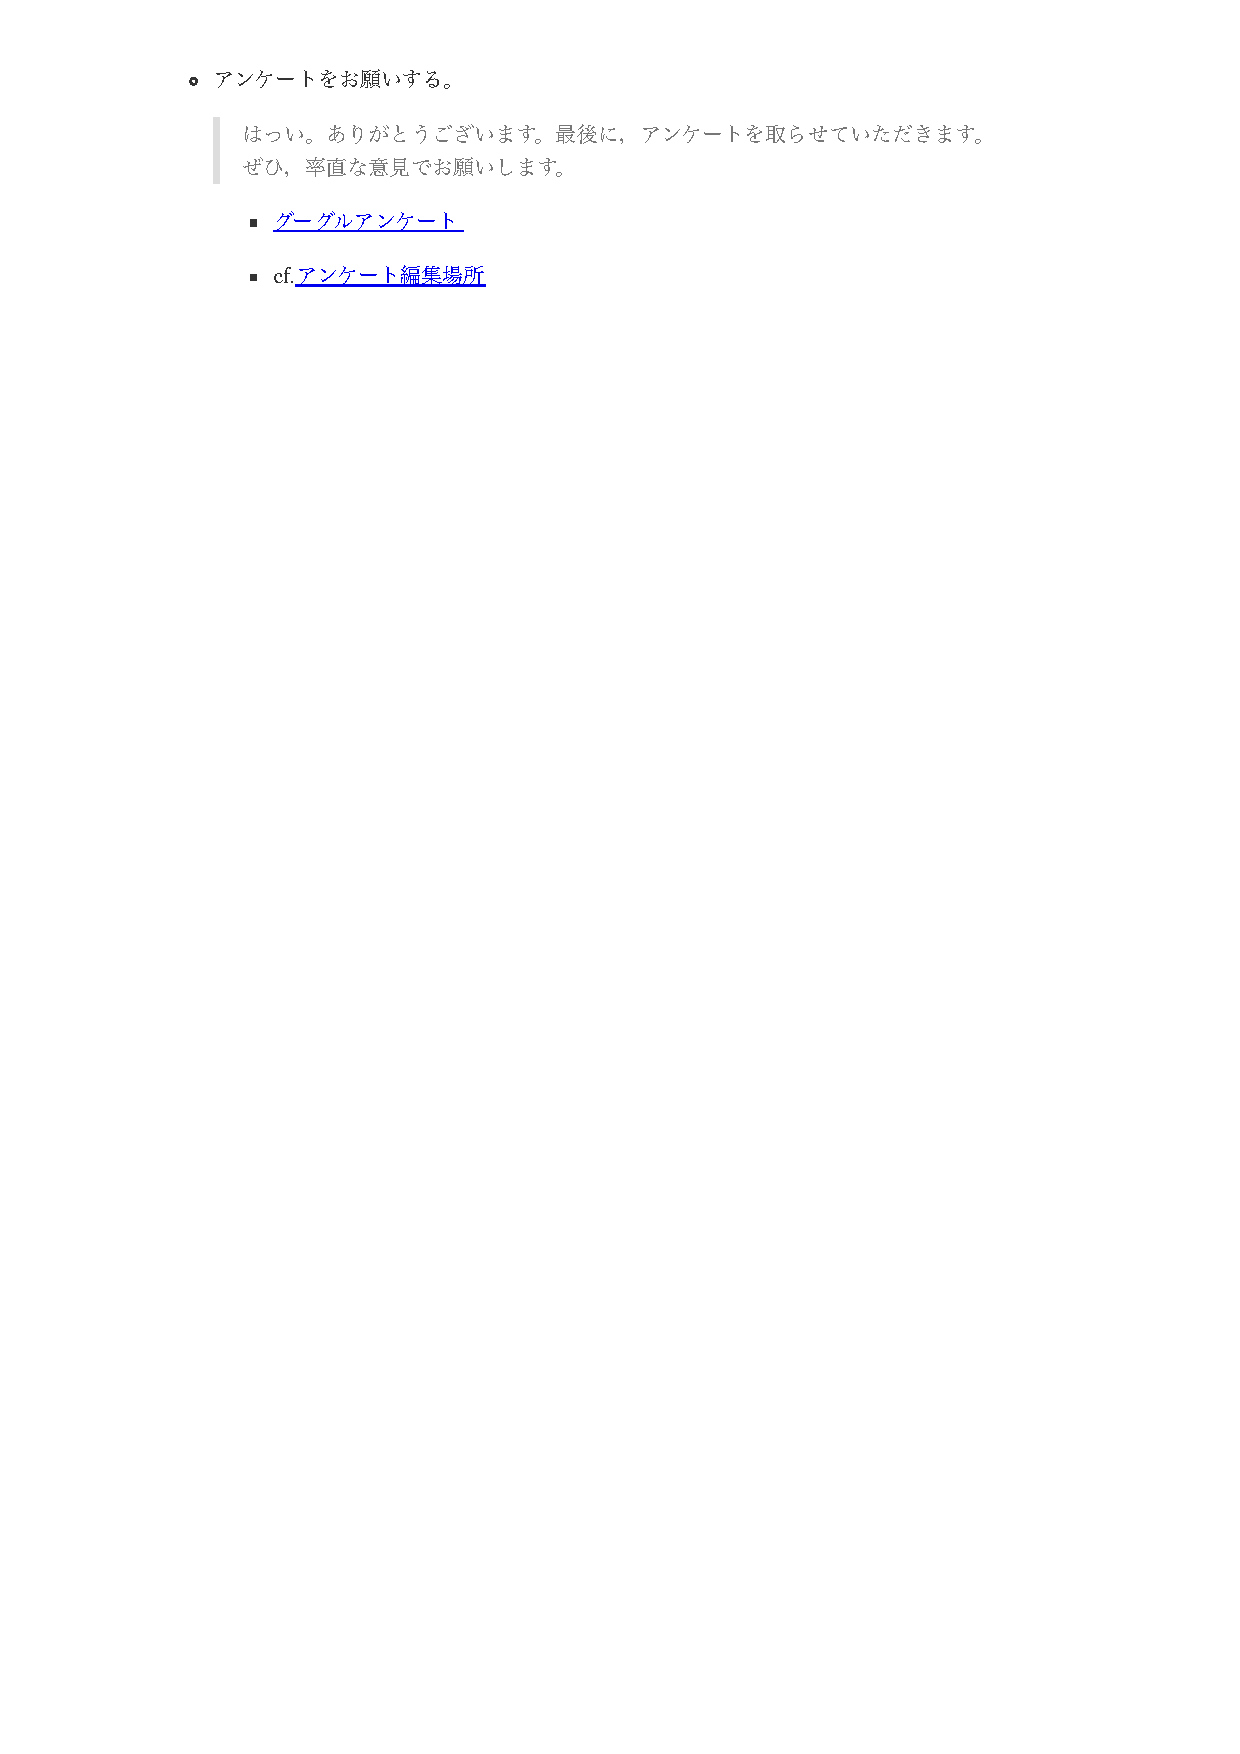
\includegraphics[width=15cm]{./fig/chapter4/inspect_2/manual/manual_3.pdf}
        \caption{検証2マニュアル3}
        \label{検証2マニュアル3}
    \end{figure}



\subsection{検証結果}
    \subsubsection{被験者について}
    \begin{itemize}
        \item 琉球大学情報工学科の学生(4人)
        \item 琉球大学情報工学科の教員(1人)
        \item 琉球大学機械システム工学科の学生(1人)
    \end{itemize}
    %琉球大学情報工学科の学生(4人)\\
    %琉球大学情報工学科の学生(1人)\\
    %琉球大学機械システム工学科の学生(1人)\\

    \subsubsection{時間の観点からの面倒さ}
        ここでは被験者に行ってもらった,登録・認証にかかる時間を以下の表\ref{検証2 認証・登録の計測時間}に示す.
        表\ref{検証2 認証・登録の計測時間} は パスワード方式,鍵方式の登録・認証それぞれについて,個の時間,平均時間を記述した表である.
        被験者6に関しては,password方式の実装の2つの問題点により,計測ができなかったため,省く.
            % 2つの問題点について
                % バグ(登録できるが,認証ができない){同じメアドで登録できてしまうから}
                % パスワード確認入力欄が無い
            %+アルファー
                % 情報工学科以外の ゆういつ の被験者 -> パソコン操作に慣れていない
                %$ --> 今後の課題として,パソコン操作に慣れていない人でも,使いやすいようにする?????
        %表の記述
        \begin{table}[htb]
            \caption{検証2\_認証・登録の計測時間}
            \label{検証2 認証・登録の計測時間}
            \begin{tabular}{|l|r|r|r|r|r|r|r|} \hline%| (ハイプ) は縦線
                %登録・認証の種類 \textbackslash 被験者 & 被験者1 & 被験者2 & 被験者3  & 被験者4 & 平均\\ \hline%\hline は横の線
                                    & 被験者5 & 被験者7 & 被験者8 & 被験者9 & 被験者10 & 被験者11 & 平均 \\ \hline%\hline は横の線
                登録(パスワード方式) & 29.68 & 20.56   & 16.20 & 42.06   & 51.85   & 17.88   & 29.71\\ \hline
                認証(パスワード方式) & 17.29 & 14.95   & 10.40 & 17.95   & 19.62   & 13.33   & 15.59\\ \hline
                登録(鍵方式)        & 11.26 & 11.06   & 8.53  & 19.18   & 12.16   & 11.98   & 12.36\\ \hline
                認証(鍵方式)        & 13.63 & 16.23   & 8.65  & 43.83   & 12.3    & 15.51   & 18.36\\ \hline
    
                %----- 最終ページの表の最下部 --------
                \multicolumn{6}{r}{\small\it (単位:秒)}\\
            \end{tabular}
        \end{table}
    
        %上の表の参考方法
        %%表\ref{検証2 認証・登録の計測時間}


    \subsubsection{アンケートの観点からの面倒さ}
        ここでは,被験者に対して,2つの方式の登録・認証が終わった直後に,
        記入してもらったアンケートについての数値のまとめを以下の表\ref{検証1 アンケートによる6段階評価}に示す.
        表\ref{検証1 アンケートによる6段階評価}は 被験者による パスワード方式,鍵方式の登録・認証それぞれについて0 〜 5 段階評価,さらに,検証自体の面倒さについての評価を加えて まとめた表である.
        被験者6に関しては,password方式の実装の2つの問題点により,時間の計測ができなかったため,省く.
        %表の記述
        \begin{table}[htb]
            \caption{検証2\_アンケートによる6段階評価}
            \label{検証2 アンケートによる6段階評価}
            \begin{tabular}{|l|r|r|r|r|r|r|r|} \hline%| (ハイプ) は縦線
                %登録・認証の種類 \textbackslash 被験者 & 被験者1 & 被験者2 & 被験者3  & 被験者4 & 平均\\ \hline%\hline は横の線
                                          & 被験者5 & 被験者7 & 被験者8 & 被験者9 & 被験者10 & 被験者11 & 平均 \\ \hline%\hline は横の線
                % 改行するために
                \begin{tabular}{l}
                    登録(パスワード方式)\\の面倒さ
                \end{tabular}
                                          & 1 & 4 & 2 & 2 & 1 & 3 & 2.17 \\ \hline%6
                % 改行するために
                \begin{tabular}{l}
                    認証(パスワード方式)\\の面倒さ  
                \end{tabular}
                                         & 1 & 3 & 2 & 2 & 2 & 3 & 2.17  \\ \hline
                登録(鍵方式)の面倒さ        & 0 & 2 & 0 & 2 & 0 & 2 & 1.00  \\ \hline
                認証(鍵方式)の面倒さ        & 1 & 1 & 1 & 2 & 1 & 2 & 1.33  \\ \hline
                検証自体の面倒さ           & 0 & 2 & 0 & 3 & 0 & 0 & 0.83  \\ \hline
    
                %----- 最終ページの表の最下部 --------
                \multicolumn{6}{r}{\small\it (0 〜 5段階)}\\
            \end{tabular}
        \end{table}
        %上の表の参考方法
        %%表\ref{検証2 アンケートによる6段階評価}


  \newpage

  \subsection{考察}
  検証者6の検証は失敗した.鍵方式の登録の検証の際,認証まで進んでしまい,データの取得ができなかったためである.
  そのことから,次の考察ができる.
    被験者6は,唯一 情報工学科でない学生であった.他の情報工学科の被験者と比較して,
    PCを専門にしていない学生である.そのことから,より利用者目線の被験者だと言える.
    利用者目線では,今回の鍵方式は使いづらい認証方式になっていると考察することができる.

    被験者7の認証(表\ref{検証2 認証・登録の計測時間})に注目すると,パスワード方式に比べて鍵方式の方が時間がかかっている.
    しかし,アンケートによる認証の面倒さ(表\ref{検証2 アンケートによる6段階評価})に着目すると,鍵方式に比べてパスワード方式の方が面倒 という数値になっている.
    また,被験者7の検証後に次のことを聞いた.「また,検証後に次のことを聞いた.「(公開鍵暗号方式方式)わかっているから,簡単だった」」
    被験者6と比較すると,鍵認証方式について次のことが考察できる.
    公開鍵暗号方式の知識を持っている人は,公開鍵暗号方式の知識を持っていない人に比べて,簡単に感じる傾向があるということが考えられる.


% 他の論文との比較
%\chapter{検証}
\label{chap:poordirection}


\section{検証1}

\subsection{検証背景}

\subsubsection{検証目的}

password認証方式の,新規登録・認証の面倒さを解決するために,第3章の提案手法で
password認証方式に変わる,公開鍵暗号方式によるssh認証を用いた,WEBサービス認証の提案を行った。\\
しかしながら,提案だけだと,新規登録・認証の面倒さを解決していることの根拠に乏しい。
よって,検証を行い,第3章の提案手法は"面倒さの軽減"に効果的に繋がっているかの確認をする。


\subsubsection{検証手段}

検証の手段としては,実際に,以下の2つの認証方式の登録・認証を被験者に体験してもらう。
%また,実験マニュアルを作成し,実験者は被験者に対して,同じように接するようにする。

\begin{itemize}
  \item バグあり,パスワード方式認証(以後 "パスワード認証"と記述する)
  \item 公開鍵暗号暗号方式によるssh認証(以後 "鍵認証”と記述する)
\end{itemize}

※バグは「認証の際に,どんなパスワードでも認証してしまう」\\
その後,2つの観点から,"面倒さ"を数値化する。
1つ目の観点は「時間」である。
"面倒さ"をアカウント登録・認証にかかる時間と推測し,計測化する。
詳しい詳細については,検証環境のマニュアルに記述する。
%まず,パスワード 形式による登録・認証の時間計測をそれぞれ行う。
% 次に,公開鍵暗号方式によるSSH 形式登録・認証の時間計測をそれぞれ行う。
% 最後に,上記の形式による時間計測を比較する。
2つ目の観点は「アンケート」である。
アンケートには,点数で答える方式,文字で記入する欄 の2つがあり,点数で答える方式により"面倒さ”を数値化する。
アンケートの細かい内容は,4.1.3の検証画面に記述する。

また,アンケートには"面倒さ"を数値化する以外にも,以下の2つの意味を込める。
1つ目の意味は次の通りである。
アカウント登録・認証にかかる時間 を,"面倒さ"と予想して検証しているが,その予想を確かめる必要がある。
アンケートを取ることにより,「アカウント登録・認証にかかる時間」と,「アンケートによる面倒さ」が比例していることを確認することで,予想を確かめることができる。
また,被験者の状態も確認することで,面倒と感じるのが,検証自体に対しての面倒さと関係があるのかを確認する。
2つ目の意味は次のとおりである。
記入欄で,改善点や感じたことの意見をもらうことで,今後の研究に生きるようなアンケートをもらう。








\subsection{検証環境}
 \subsubsection{検証場所}
 第3章で記述したとおり,検証場所は学科のVMを用いているため,学科のネットワーク内(有線LAN,wifiアクセスポイント{ie-ryukyu})
 から,アクセスして検証を行う。


 %\subsubsection{検証画面}

 \subsubsection{検証の流れ}
    ここでは,被験者に行ってもらう,検証の流れを記述する。
    時間の観点で"面倒さ"を数値化する検証では,被験者にはパスワード方式,鍵方式の登録・認証をそれぞれ行ってもらう。その時,被験者は時間を測る。 
    また,再現性を持って,検証を行うためにマニュアルを作成し,マニュアル通りに検証を行う。
    アンケートの観点で"面倒さ"を数値化する検証では,
    時間の観点で"面倒さ"を数値化する検証 が終わった直後に行うようにすることで,被験者の思った感情とアンケート結果の差異が少なくなるようにする。
  

  \subsubsection{検証画面}
    %実際に記述--------------------------------------------------------
    ここでは,被験者に行ったもらう検証画面をのせる。

    以下の
    図\ref{検証1アカウント作成(パスワード方式)},
    図\ref{検証1認証(パスワード方式)}
    図\ref{検証1認証成功後(パスワード方式)}
    は,第3章の提案手法で実現したパスワード方式,登録・認証を,実際に被験者に行ってもらった時のブラウザ画面である。
    図\ref{検証1アカウント作成(パスワード方式)}は,アカウント登録画面である。
    図\ref{検証1認証(パスワード方式)}は,図\ref{検証1アカウント作成(パスワード方式)}で登録したアカウントに認証するための画面である。
    図\ref{検証1認証成功後(パスワード方式)}は,図\ref{検証1認証(パスワード方式)}で認証成功した後の画面である。
    % パスワード方式のスクショ---------------------------
    \vspace{4cm}%図の位置を正しくする!
    %\begin{figure}[h]
    \begin{figure}[H]
        %\centering
        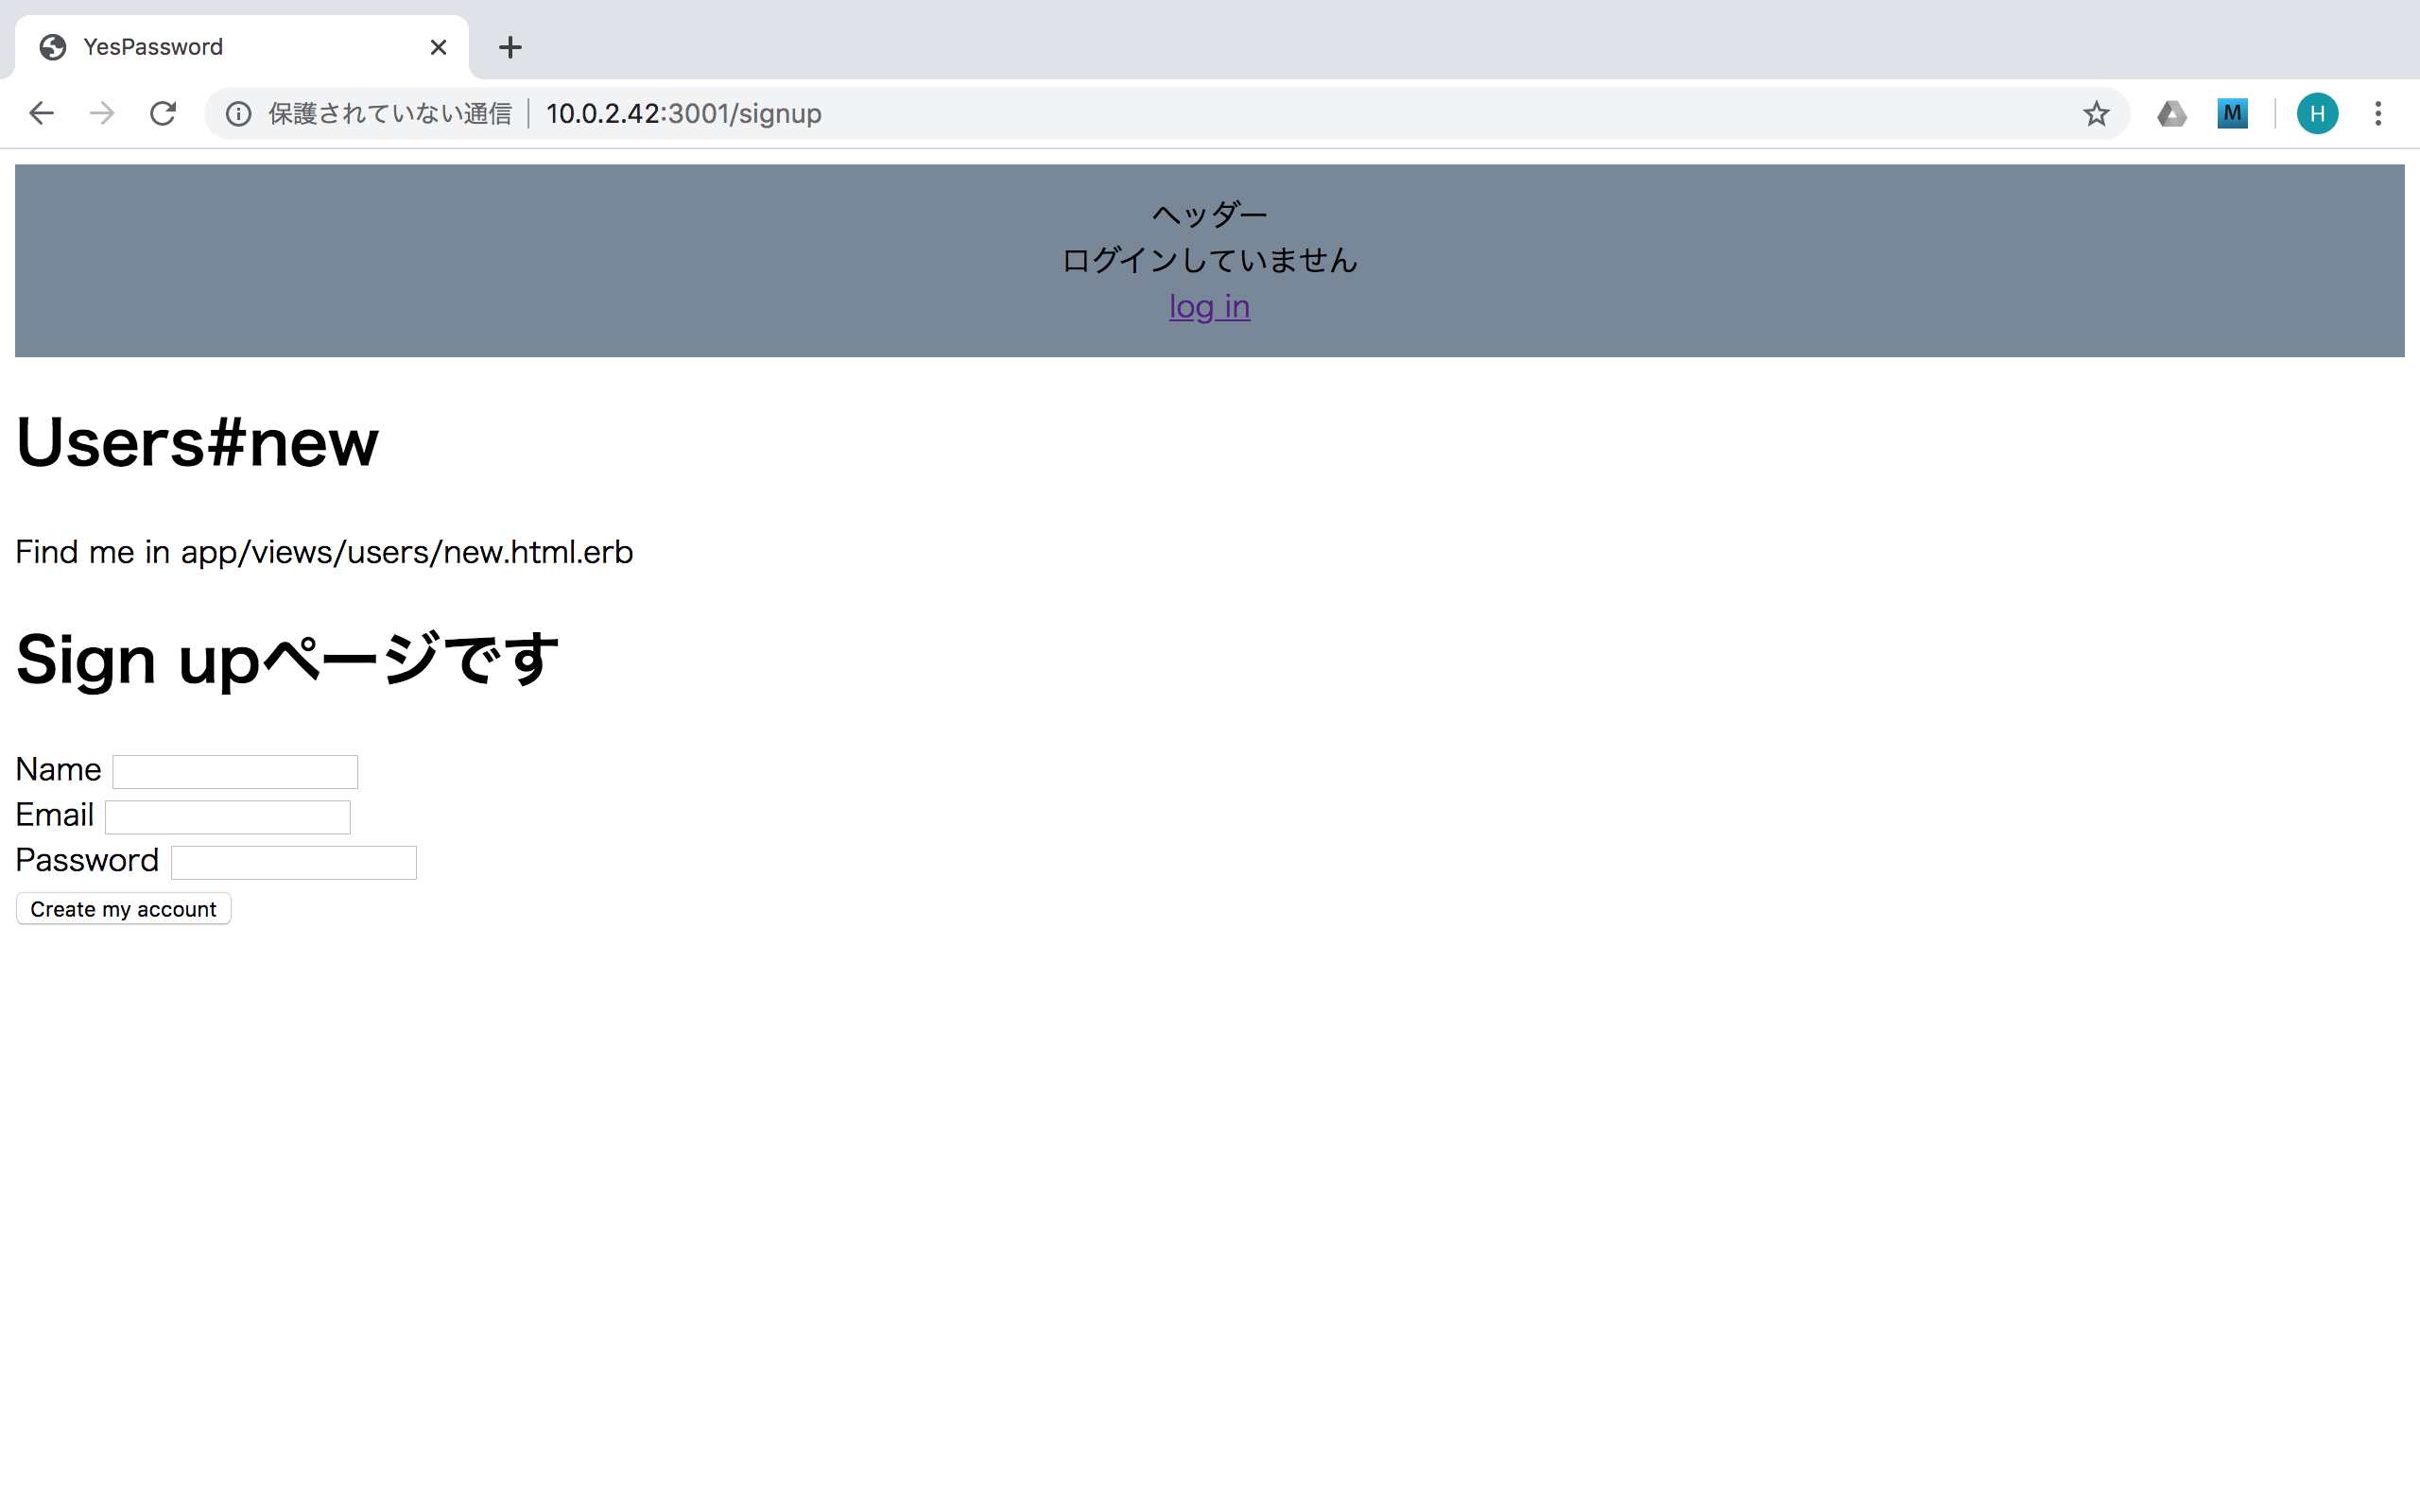
\includegraphics[height=8.4cm]{./fig/chapter4/inspect_1/password_screnn/sign_up.png}
        \caption{検証1\_アカウント作成(パスワード方式)}
        \label{検証1アカウント作成(パスワード方式)}
    \end{figure}

    \vspace{4cm}%図の位置を正しくする!
    \begin{figure}[H]
        %\centering
        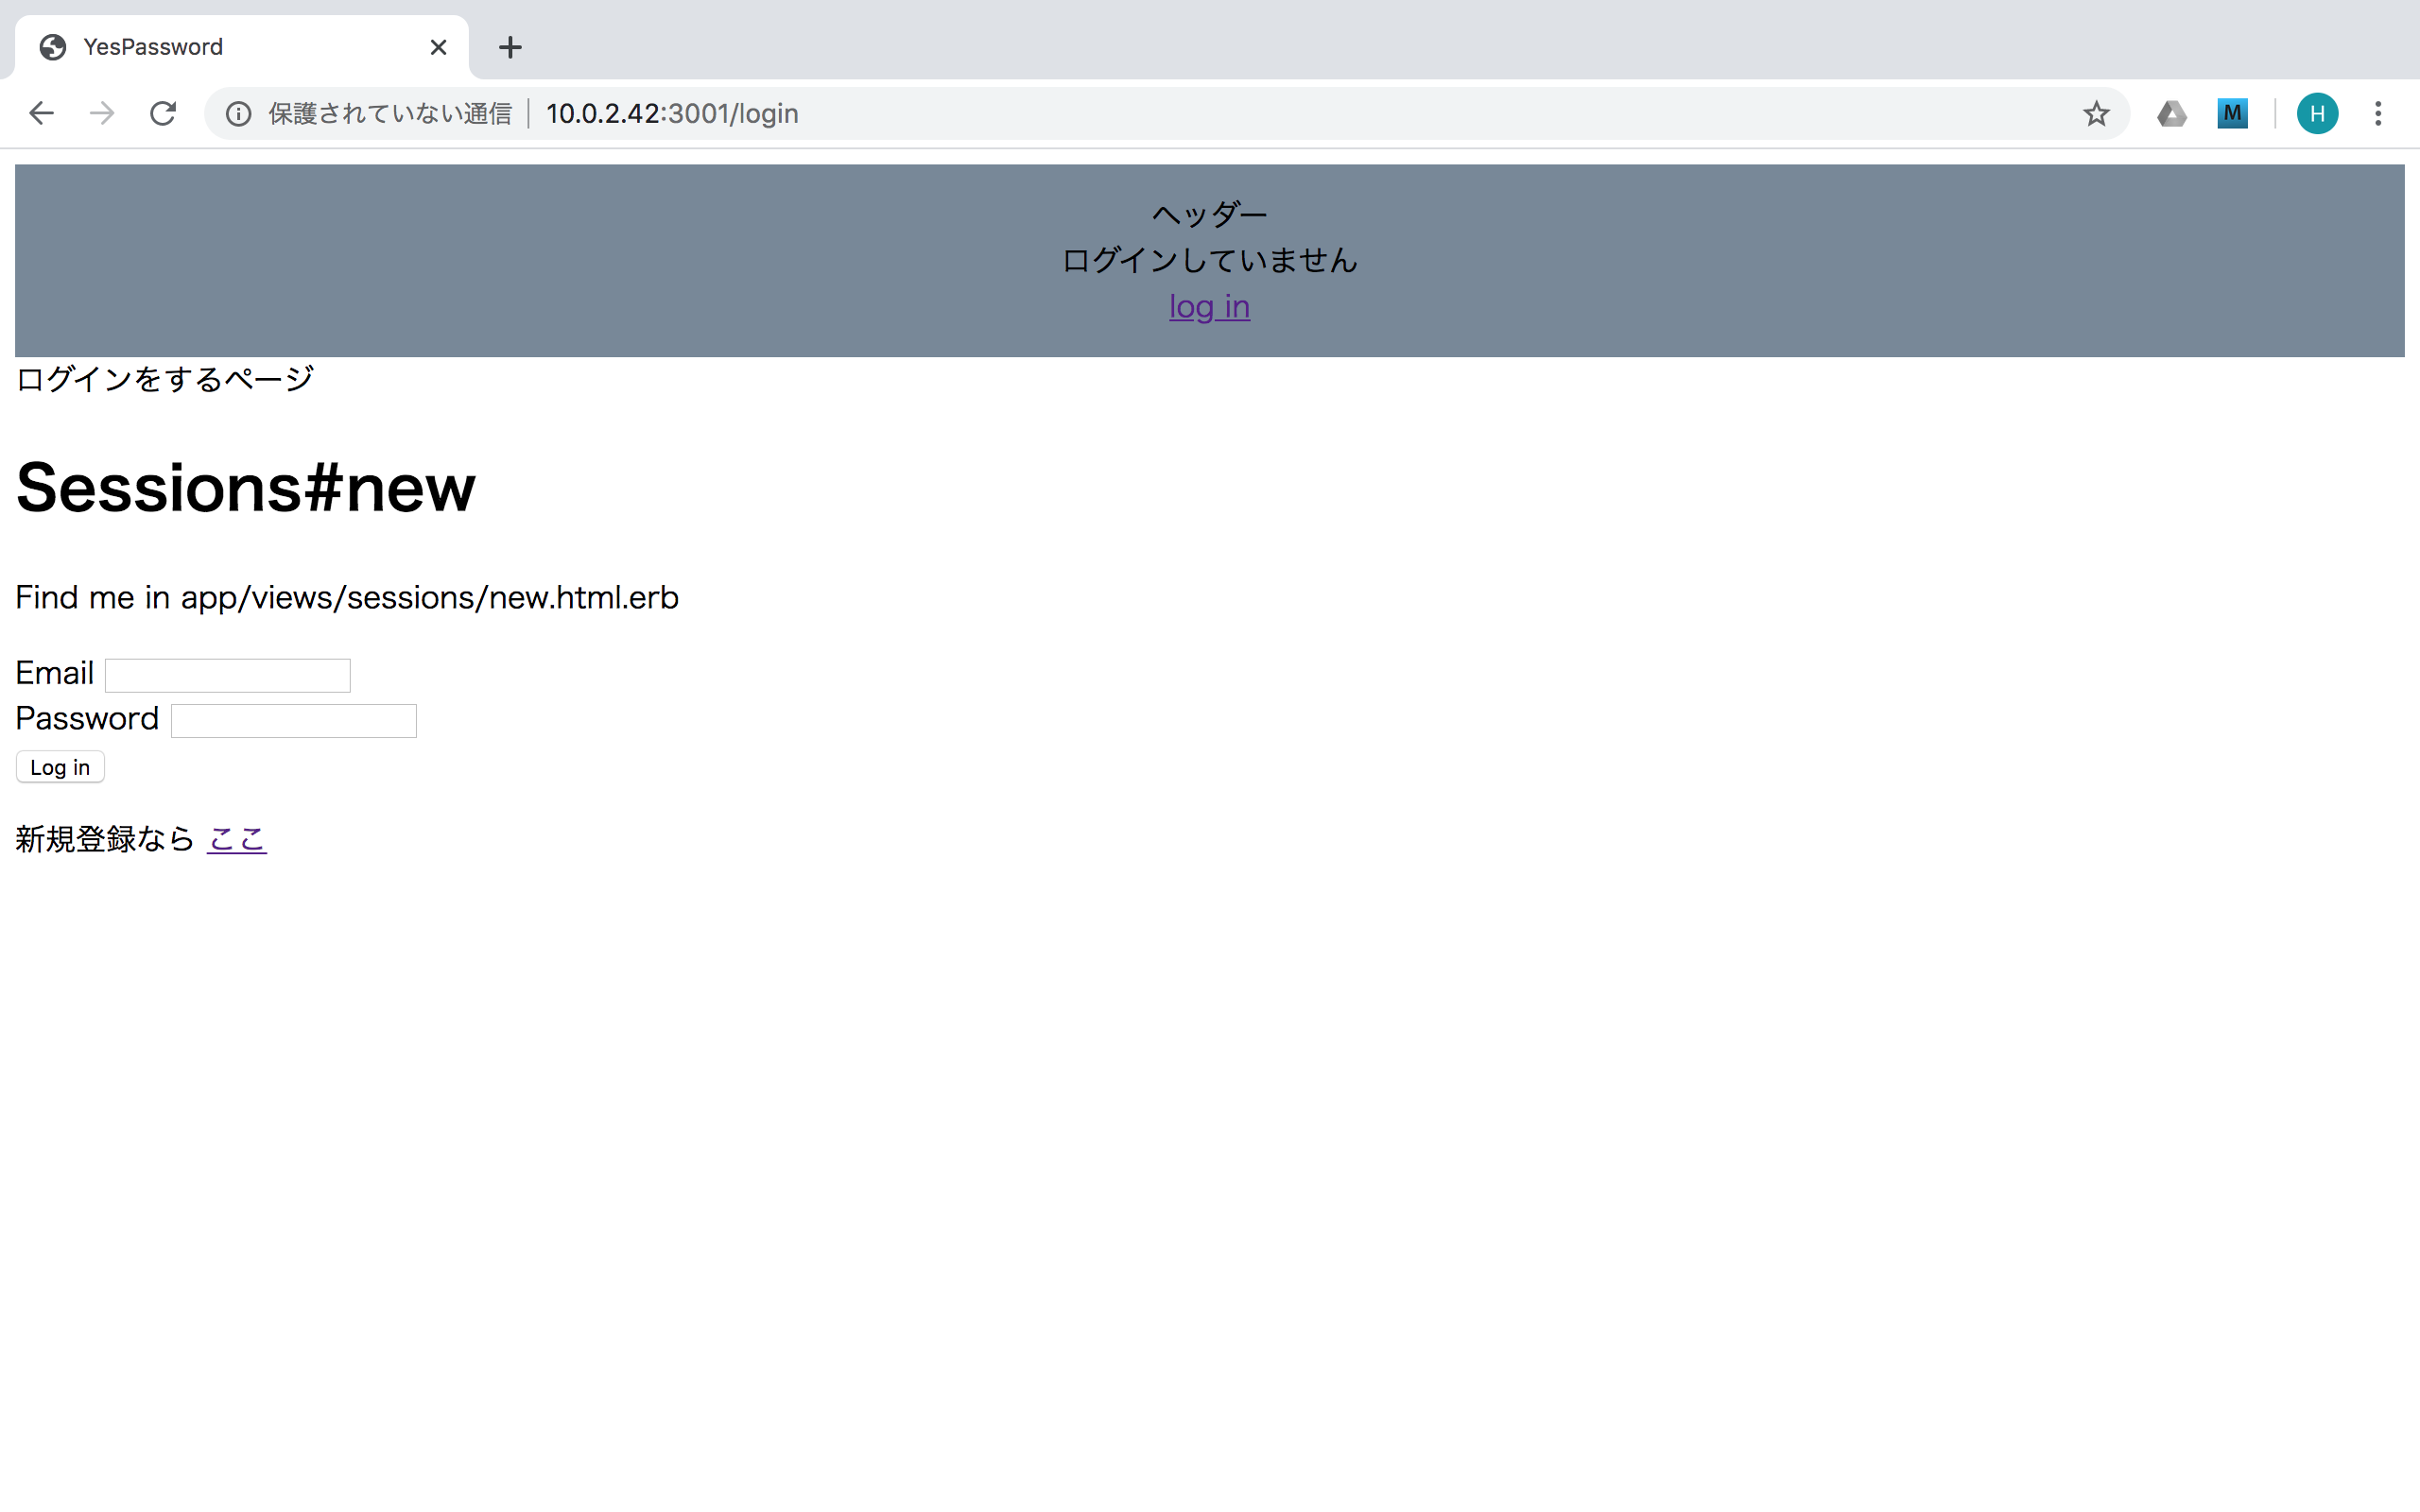
\includegraphics[height=8.4cm]{./fig/chapter4/inspect_1/password_screnn/login.png}
        \caption{検証1\_認証(パスワード方式)}
        \label{検証1認証(パスワード方式)}
    \end{figure}

    \vspace{4cm}%図の位置を正しくする!
    \begin{figure}[H]
        %\centering
        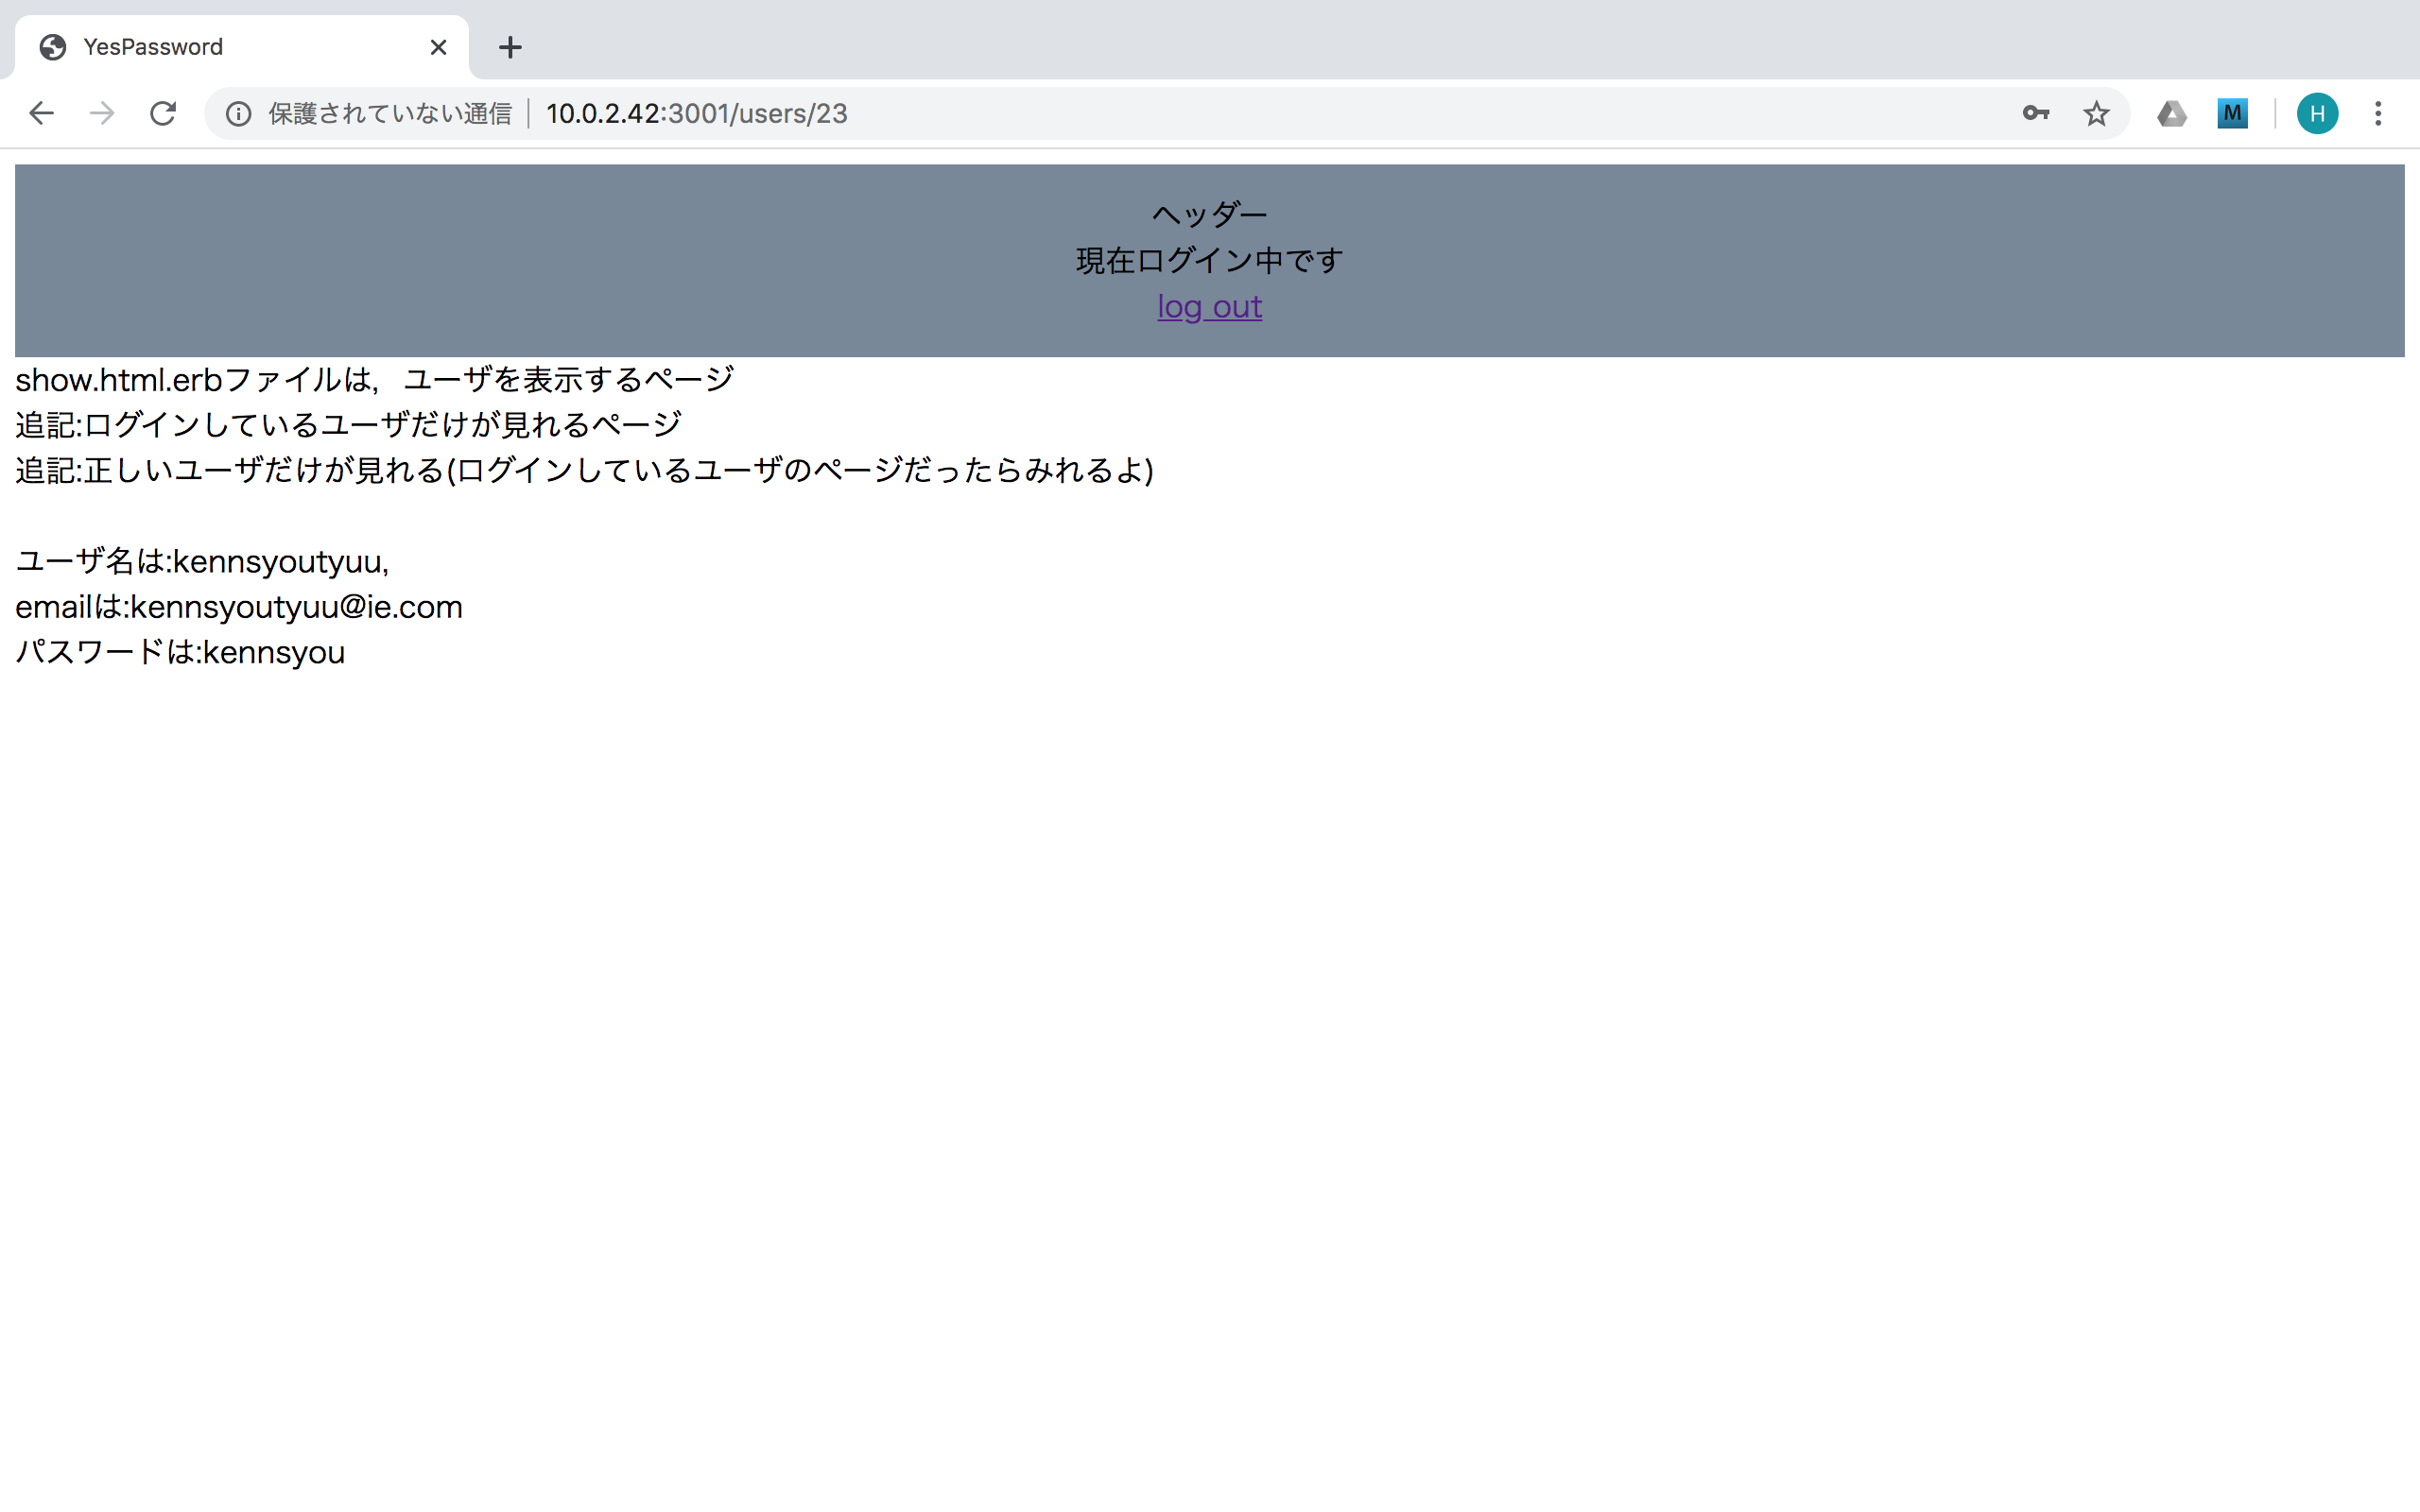
\includegraphics[height=8.4cm]{./fig/chapter4/inspect_1/password_screnn/success.png}
        \caption{検証1\_認証成功後(パスワード方式)}
        \label{検証1認証成功後(パスワード方式)}
    \end{figure}
    % パスワード方式のスクショ---------------------------








    \newpage
    \newpage

    以下の
    図\ref{検証1アカウント作成(鍵方式)},
    図\ref{検証1認証(鍵方式)}
    図\ref{検証1認証成功後(鍵方式)}
    は,第3章の提案手法で実現した,鍵方式の登録・認証を,実際に被験者に行ってもらった時のブラウザ画面である。
    図\ref{検証1アカウント作成(鍵方式)}は,アカウント登録画面である。
    図\ref{検証1認証(鍵方式)}は,図\ref{検証1アカウント作成(鍵方式)}で登録したアカウントに認証するための画面である。
    図\ref{検証1認証成功後(鍵方式)}は,図\ref{検証1認証(鍵方式)}で認証成功した後の画面である。
    % 鍵方式のスクショ----------------------------------
    \vspace{4cm}%図の位置を正しくする!
    \begin{figure}[H]
        %\centering
        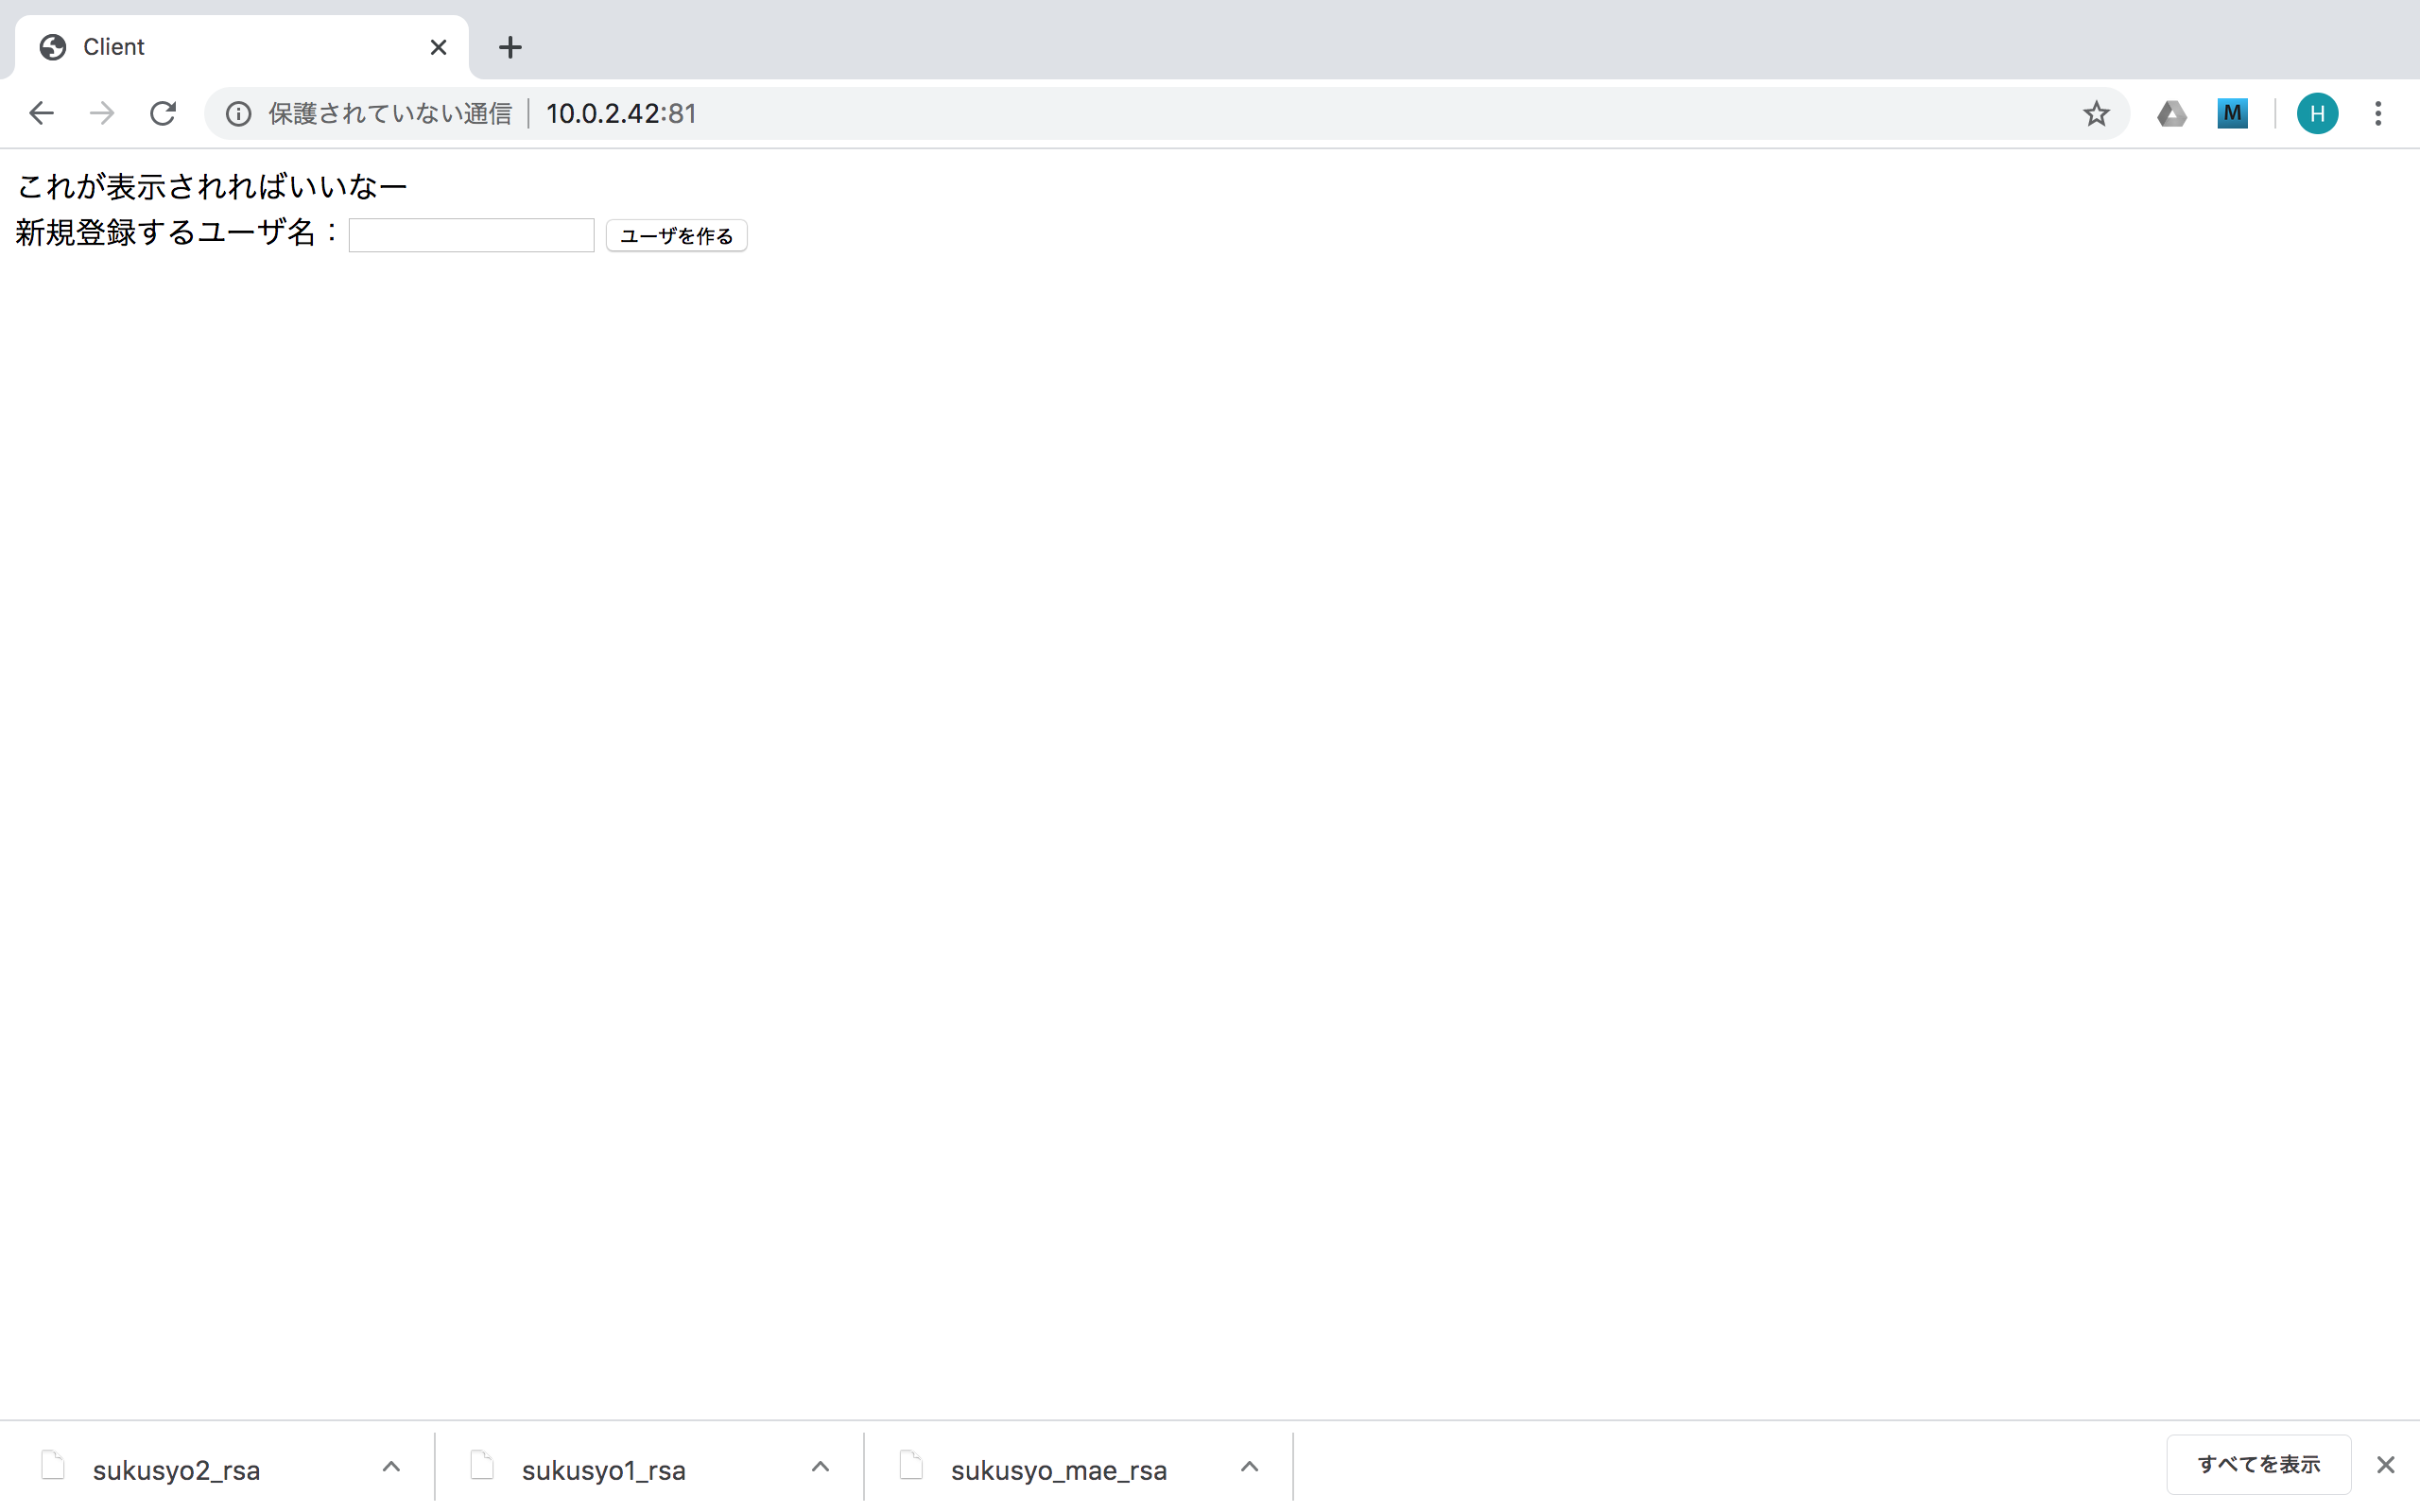
\includegraphics[height=8.4cm]{./fig/chapter4/inspect_1/key_screnn/sign_up.png}
        \caption{検証1\_アカウント作成(鍵方式)}
        \label{検証1アカウント作成(鍵方式)}
    \end{figure}

    \vspace{4cm}%図の位置を正しくする!
    \begin{figure}[H]
        %\centering
        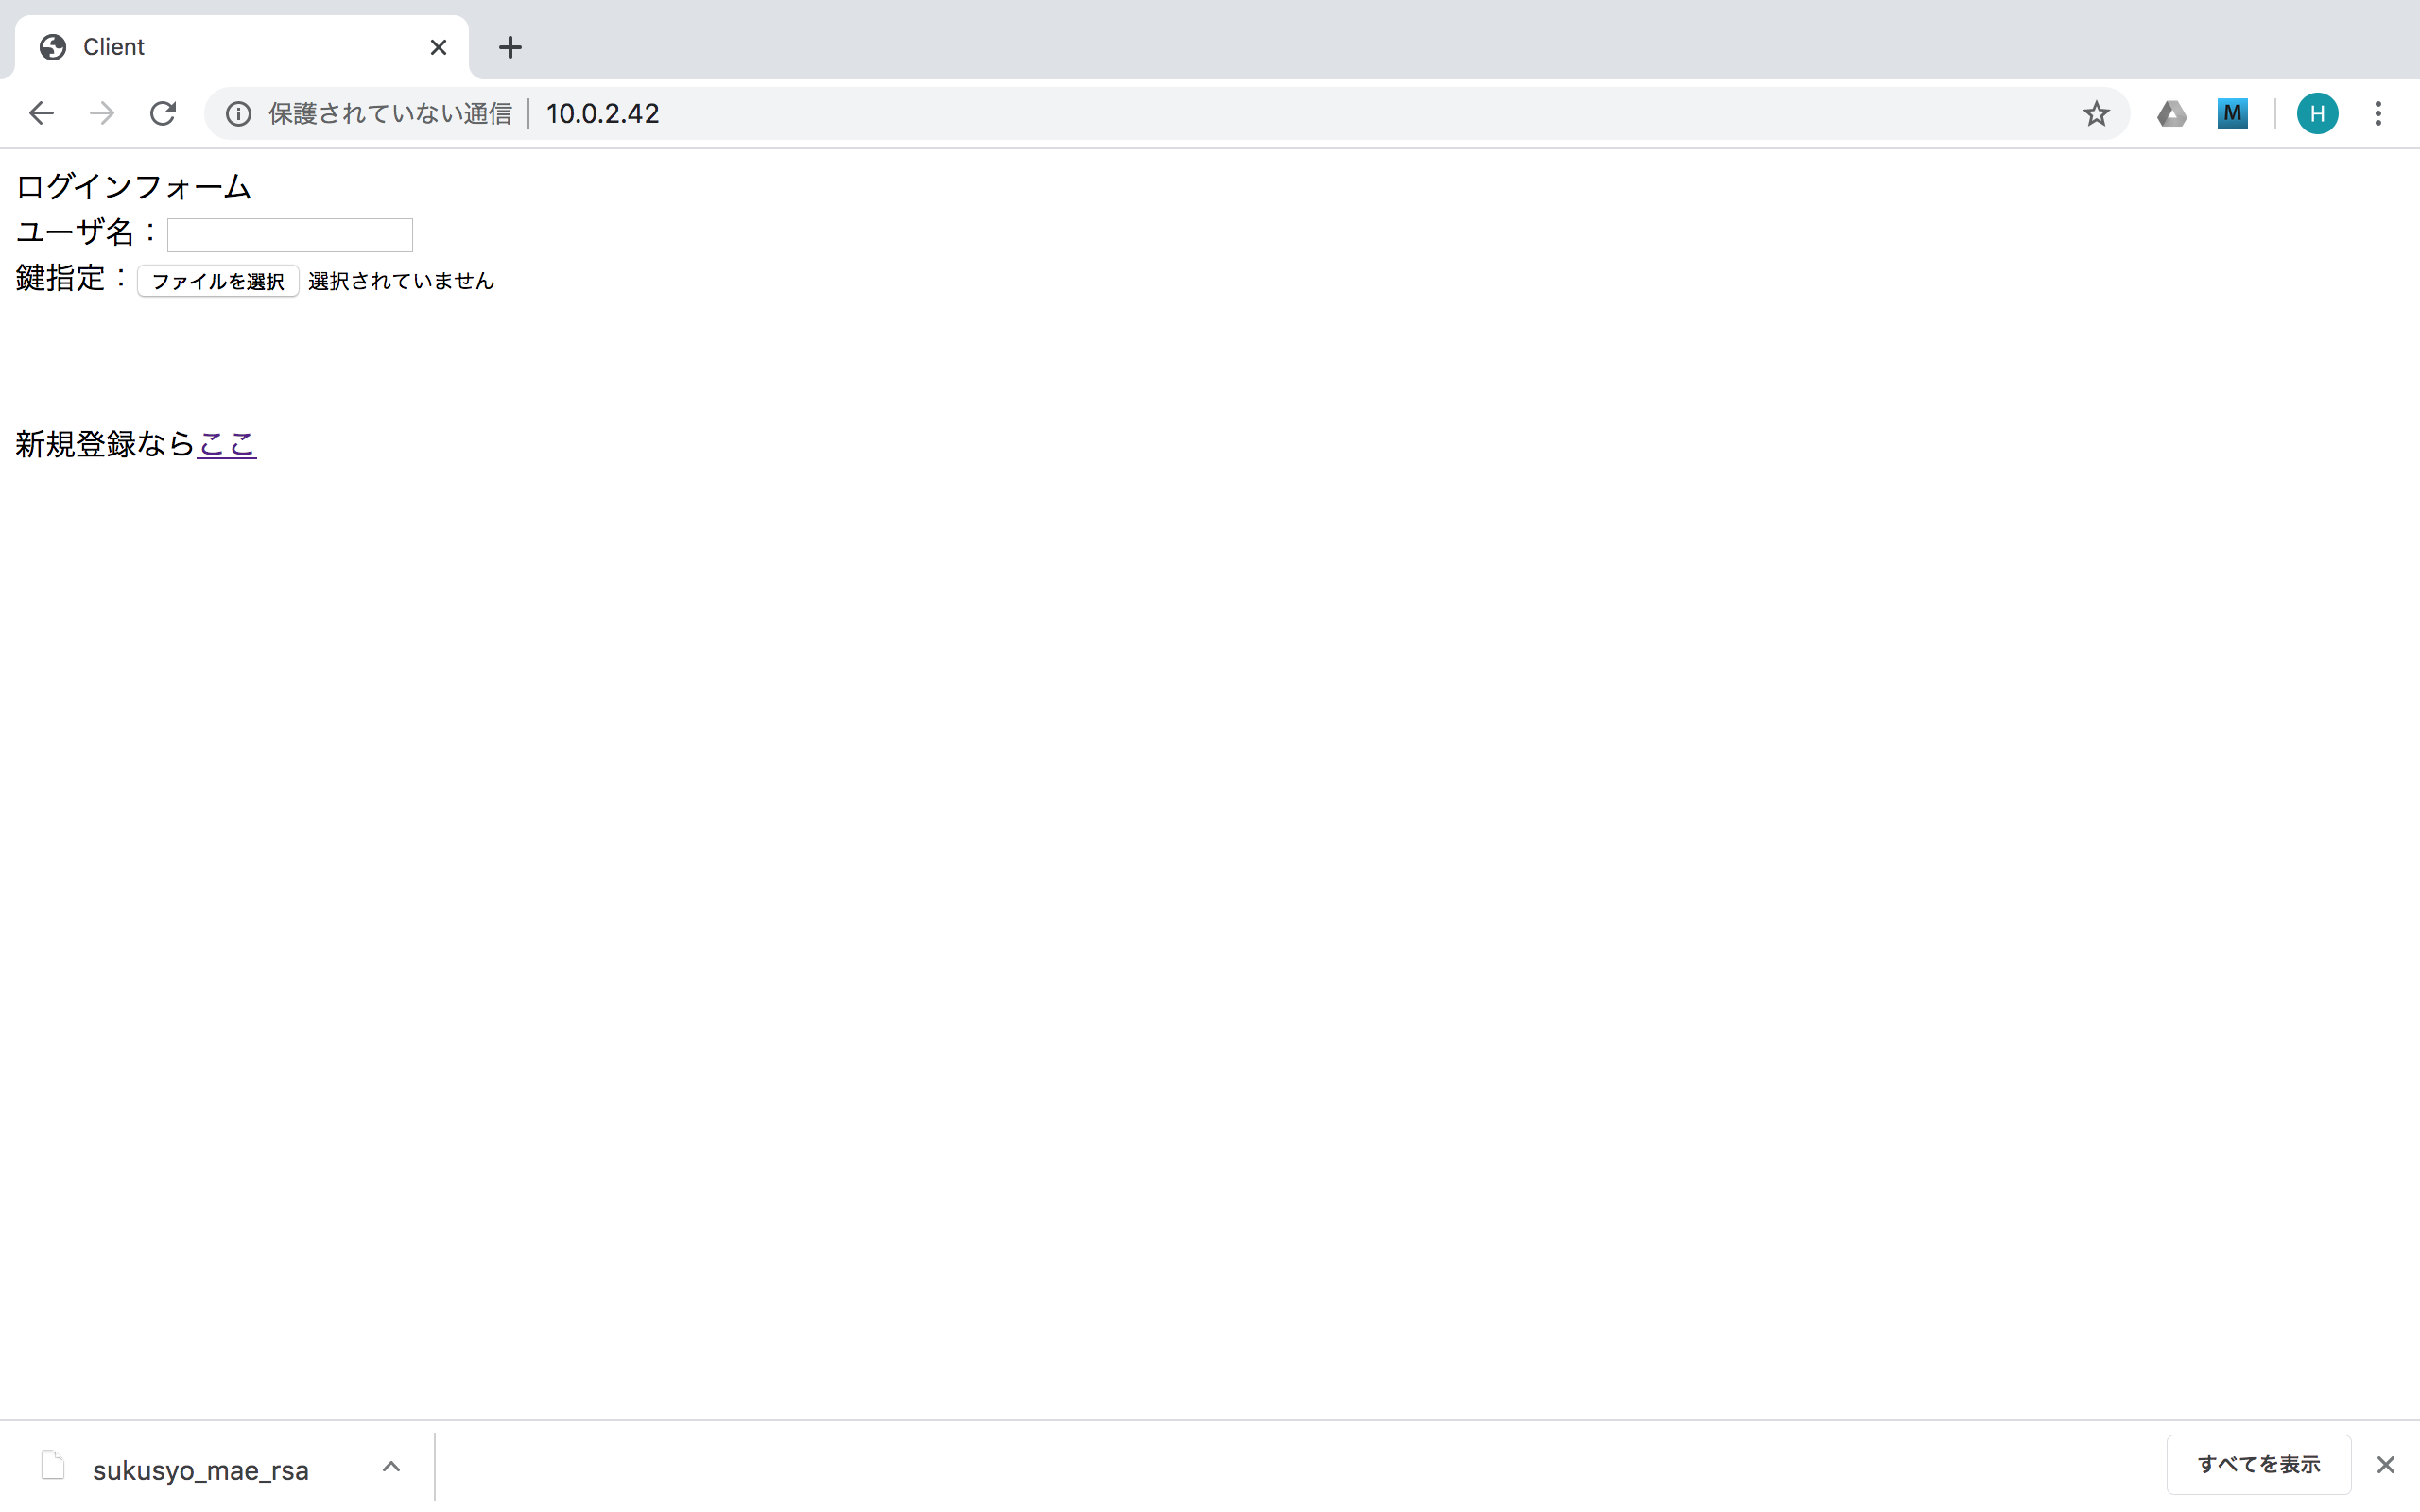
\includegraphics[height=8.4cm]{./fig/chapter4/inspect_1/key_screnn/login.png}
        \caption{検証1\_認証(鍵方式)}
        \label{検証1認証(鍵方式)}
    \end{figure}

    \vspace{4cm}%図の位置を正しくする!
    \begin{figure}[H]
        %\centering
        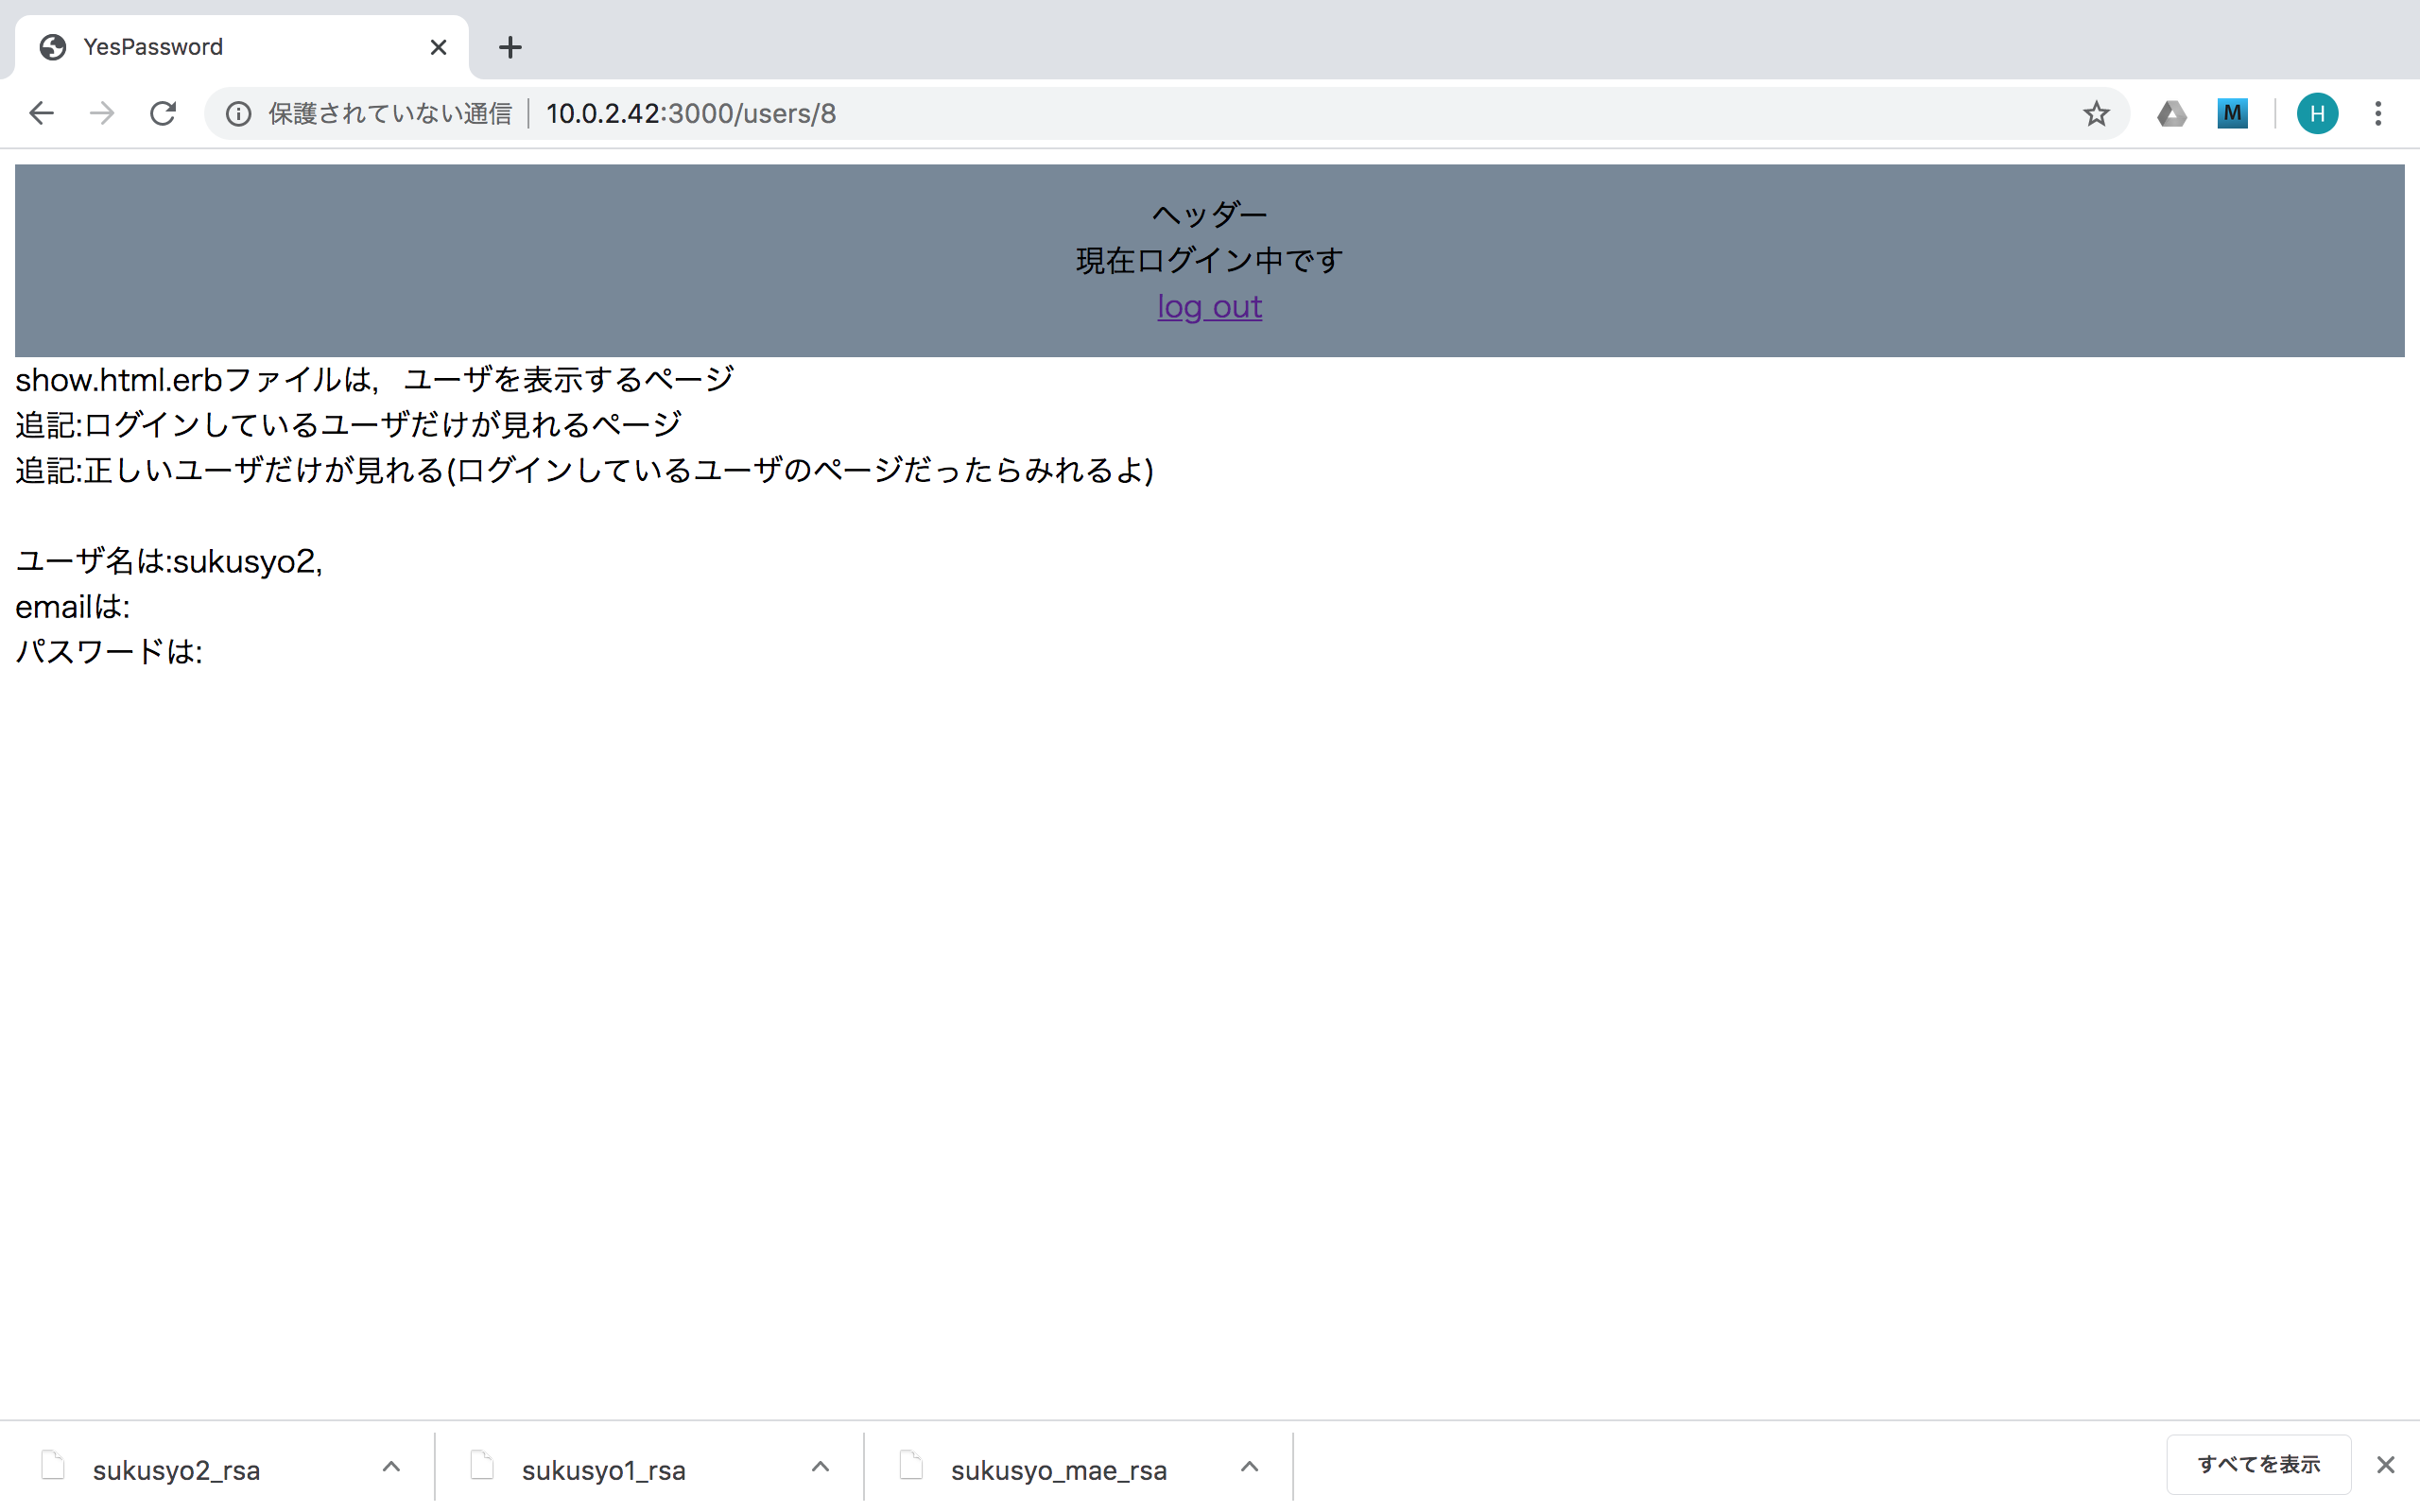
\includegraphics[height=8.4cm]{./fig/chapter4/inspect_1/key_screnn/login-after2.png}
        \caption{検証1\_認証成功後(鍵方式)}
        \label{検証1認証成功後(鍵方式)}
    \end{figure}
    % 鍵方式のスクショ----------------------------------





    

    以下の
    図\ref{アンケート1},
    図\ref{アンケート2},
    図\ref{アンケート3},
    図\ref{アンケート4}
    は
    図\ref{検証1アカウント作成(パスワード方式)} 〜 図\ref{検証1認証成功後(鍵方式)} までの,
    時間計測が終わった直後に行う,アンケートの画面である。
    %% アンケートの意図を説明
    % 検証自体面倒か
    図\ref{アンケート1} では,"検証自体の面倒さ"をアンケートで聞いている。
    その意図として,"面倒"と感じた感情は,検証役になること自体が面倒だったことに起因していないかを確かめるためである。
    % 登録・認証に対して,面倒と感じた度合いを
    図\ref{アンケート2}では,パスワード方式の登録・認証それぞれについて,どのくらい面倒かを質問している。
    図\ref{アンケート3}では,鍵方式の登録・認証それぞれについて,どのくらい面倒かを質問している。
    図\ref{アンケート2},図\ref{アンケート3}の質問の意図としては,アンケートの観点から"面倒さ"を数値化することである。
    図\ref{アンケート4}では,鍵方式の登録・認証について,被験者の技術視点と利用視点から,自由形式で意見を求めている。
    図\ref{アンケート4}の意図としては,よりよい物を作るために,被験者意見を収集し,今後の方針を決めるためである。

    % アンケートのスクショ----------------------------------
    \vspace{4cm}%図の位置を正しくする!
    \begin{figure}[H]
        %\centering
        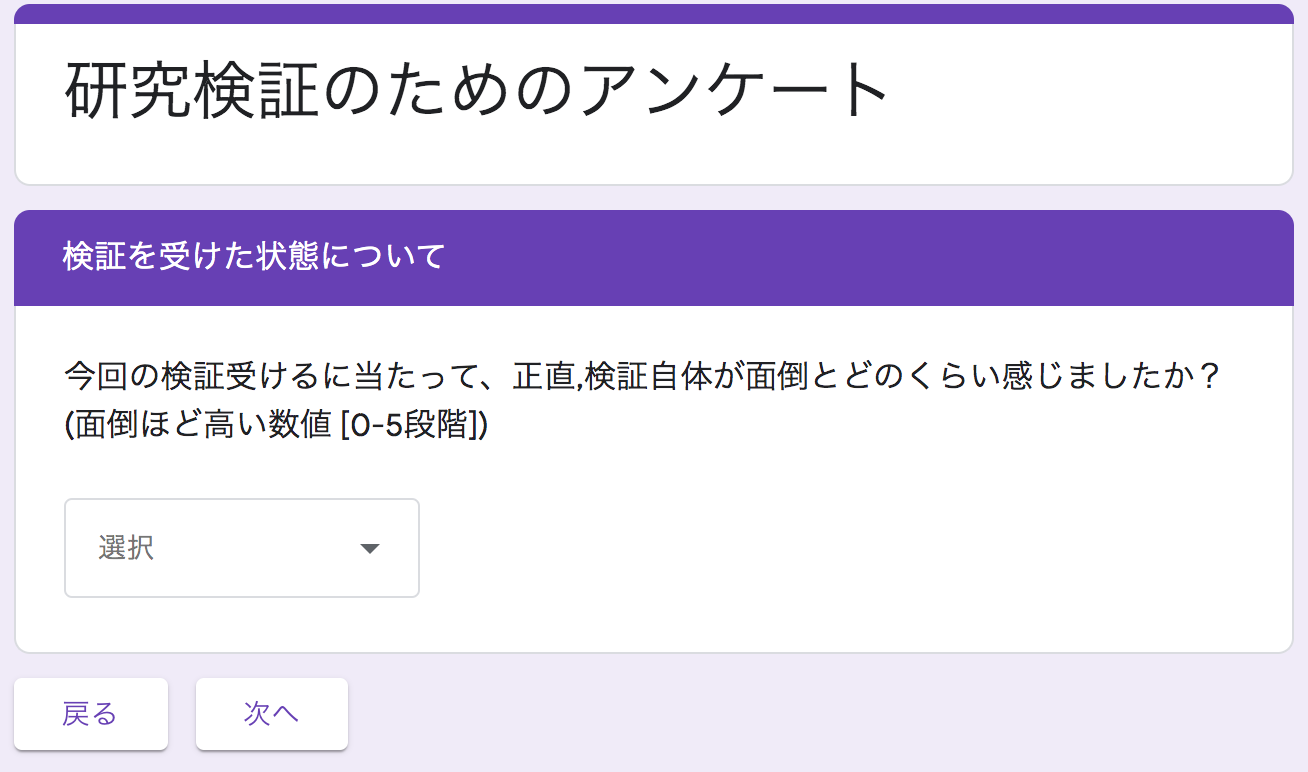
\includegraphics[width=15cm]{./fig/chapter4/inspect_1/questionnaire/questionnaire_1.png}
        \caption{アンケート1}
        \label{アンケート1}
    \end{figure}

    \vspace{4cm}%図の位置を正しくする!
    \begin{figure}[H]
        %\centering
        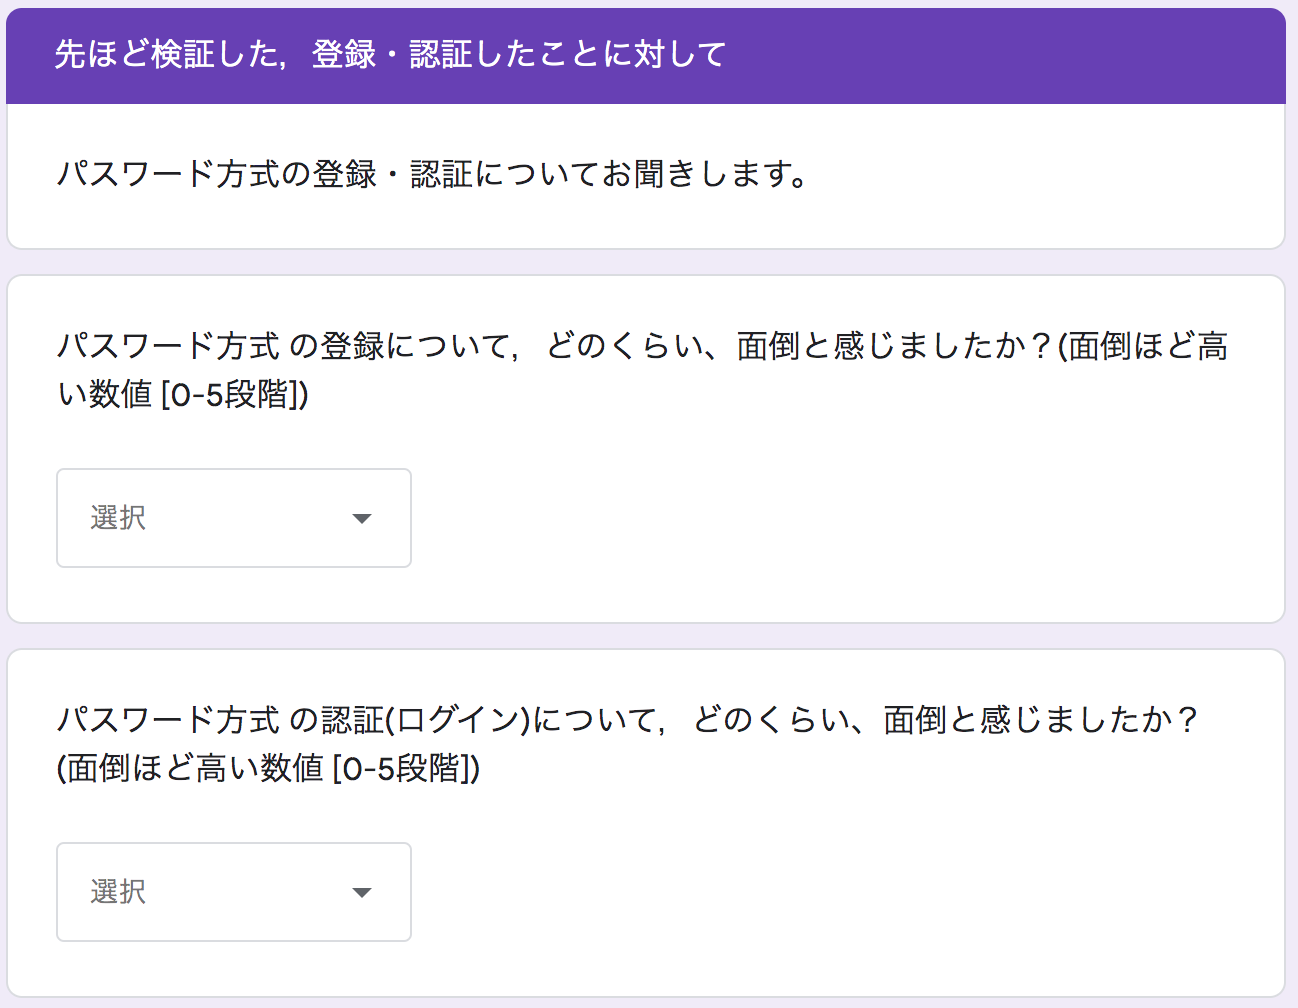
\includegraphics[width=15cm]{./fig/chapter4/inspect_1/questionnaire/questionnaire_2.png}
        \caption{アンケート2}
        \label{アンケート2}
    \end{figure}

    \vspace{4cm}%図の位置を正しくする!
    \begin{figure}[H]
        %\centering
        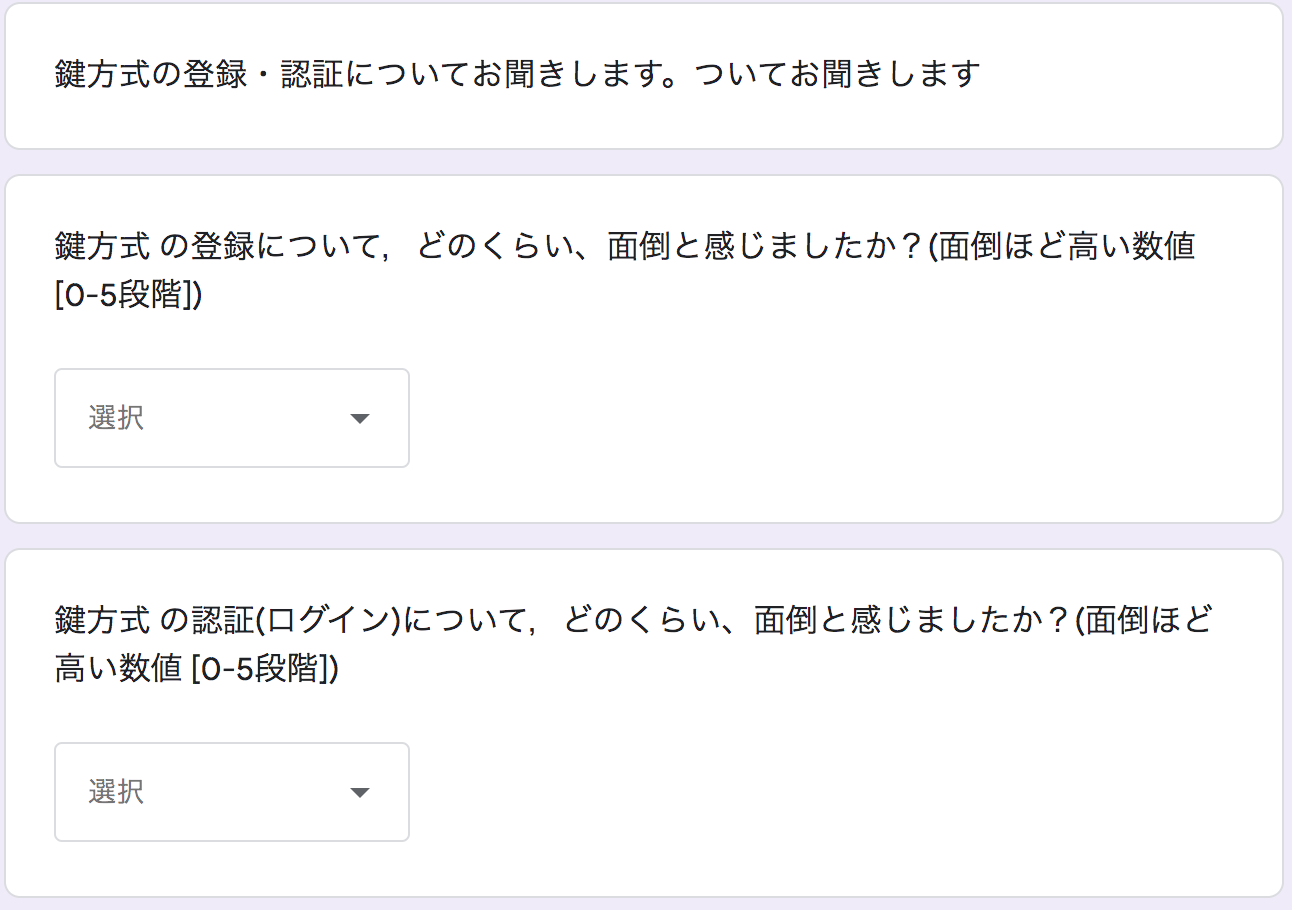
\includegraphics[width=15cm]{./fig/chapter4/inspect_1/questionnaire/questionnaire_3.png}
        \caption{アンケート3}
        \label{アンケート3}
    \end{figure}

    \vspace{4cm}%図の位置を正しくする!
    \begin{figure}[H]
        %\centering
        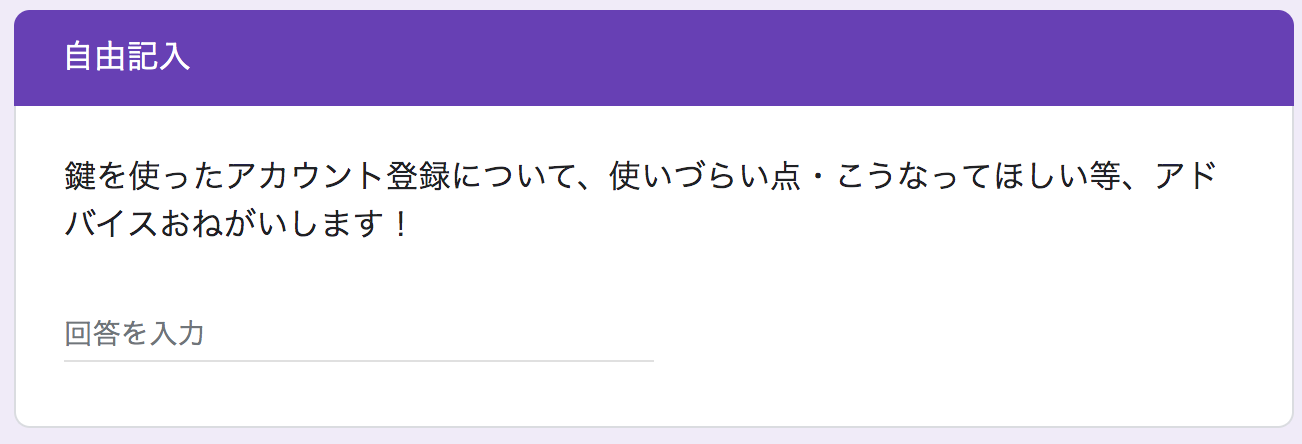
\includegraphics[width=15cm]{./fig/chapter4/inspect_1/questionnaire/questionnaire_4.png}
        \caption{アンケート4}
        \label{アンケート4}
    \end{figure}

    
    % アンケートのスクショ----------------------------------

    %実際に記述--------------------------------------------------------
    




    %%%%%%%%%%%%%%%%%%%%%%%%%%%アン
    %目的
    %  ここでは,被験者に行ったもらう検証画面をのせる。
    %  %(なぜか --> 
    %  % - 検証結果が,どういう検証をした上での,結果になったかを見る必要がある。
    %  % - プラスアルファ
    %  %   - 検証結果を受けて,変更したから,どういう変更したかを,被験者目線でわかるようにする
    %  %)
    %  
    %検証の詳細
    %  パスワード方式の認証・登録の検証画面
    %  鍵方式の認証・登録の検証画面
    %  アンケートの画面
    %
    %  
    %被験者に検証してもらう,鍵方式とパスワード方式それぞれの,登録・認証をする上での,図を載せる。
    %
    %%%%%%%%%%%%%%%%%%%%%%%%%%%アン

 \subsubsection{検証マニュアル}
 %再現性のためにという説明をする
 以下の図\ref{検証マニュアル1},図\ref{検証マニュアル2}は,上記の図\ref{検証1アカウント作成(パスワード方式)} 〜 図\ref{アンケート4} 
 の検証を行うためのマニュアルである.
 マニュアルを作成して,検証を行った意図としては,再現性を持って検証を行うためである.

 \newpage

 \vspace{4cm}%図の位置を正しくする!
 \begin{figure}[H]
     %\centering
     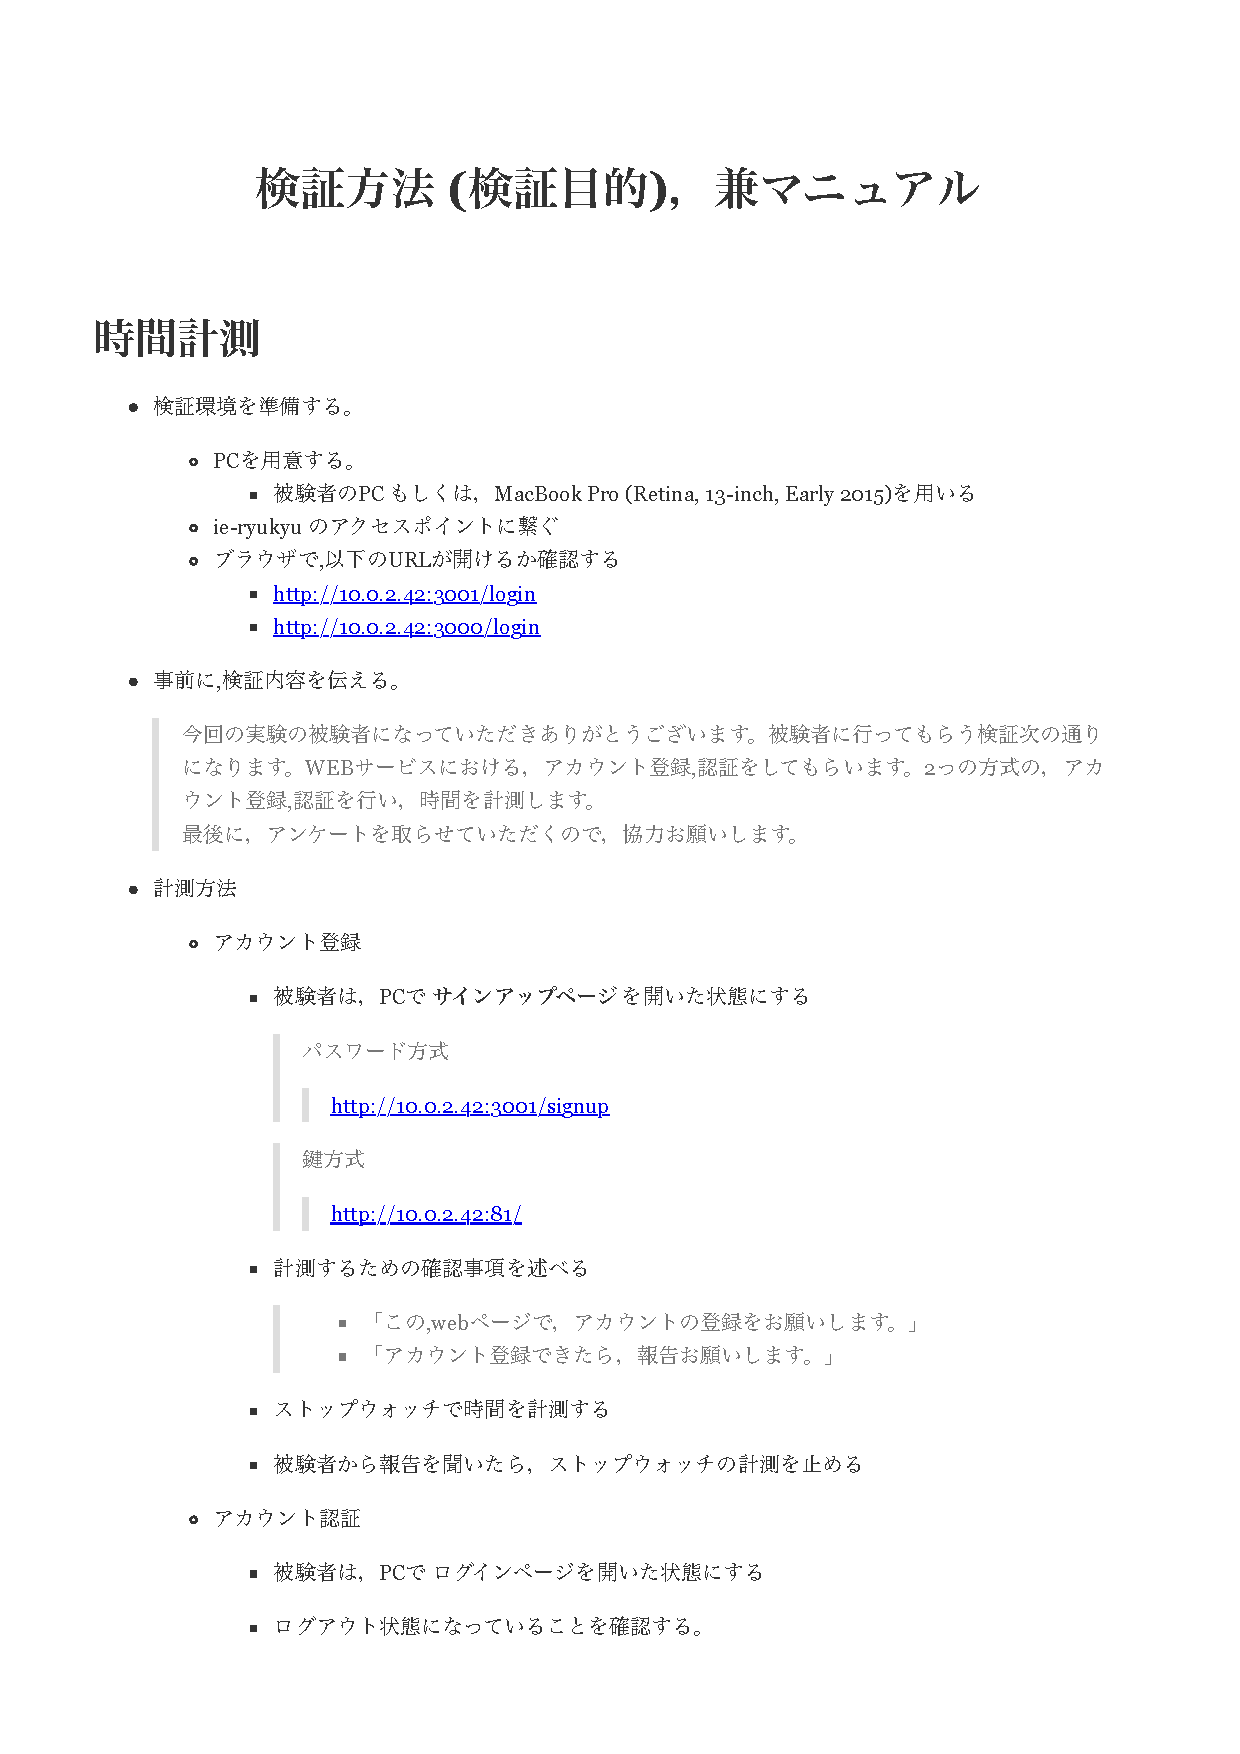
\includegraphics[width=15cm]{./fig/chapter4/inspect_1/manual/manual_1.pdf}
     \caption{検証マニュアル1}
     \label{検証マニュアル1}
 \end{figure}

 \vspace{4cm}%図の位置を正しくする!
 \begin{figure}[H]
     %\centering
     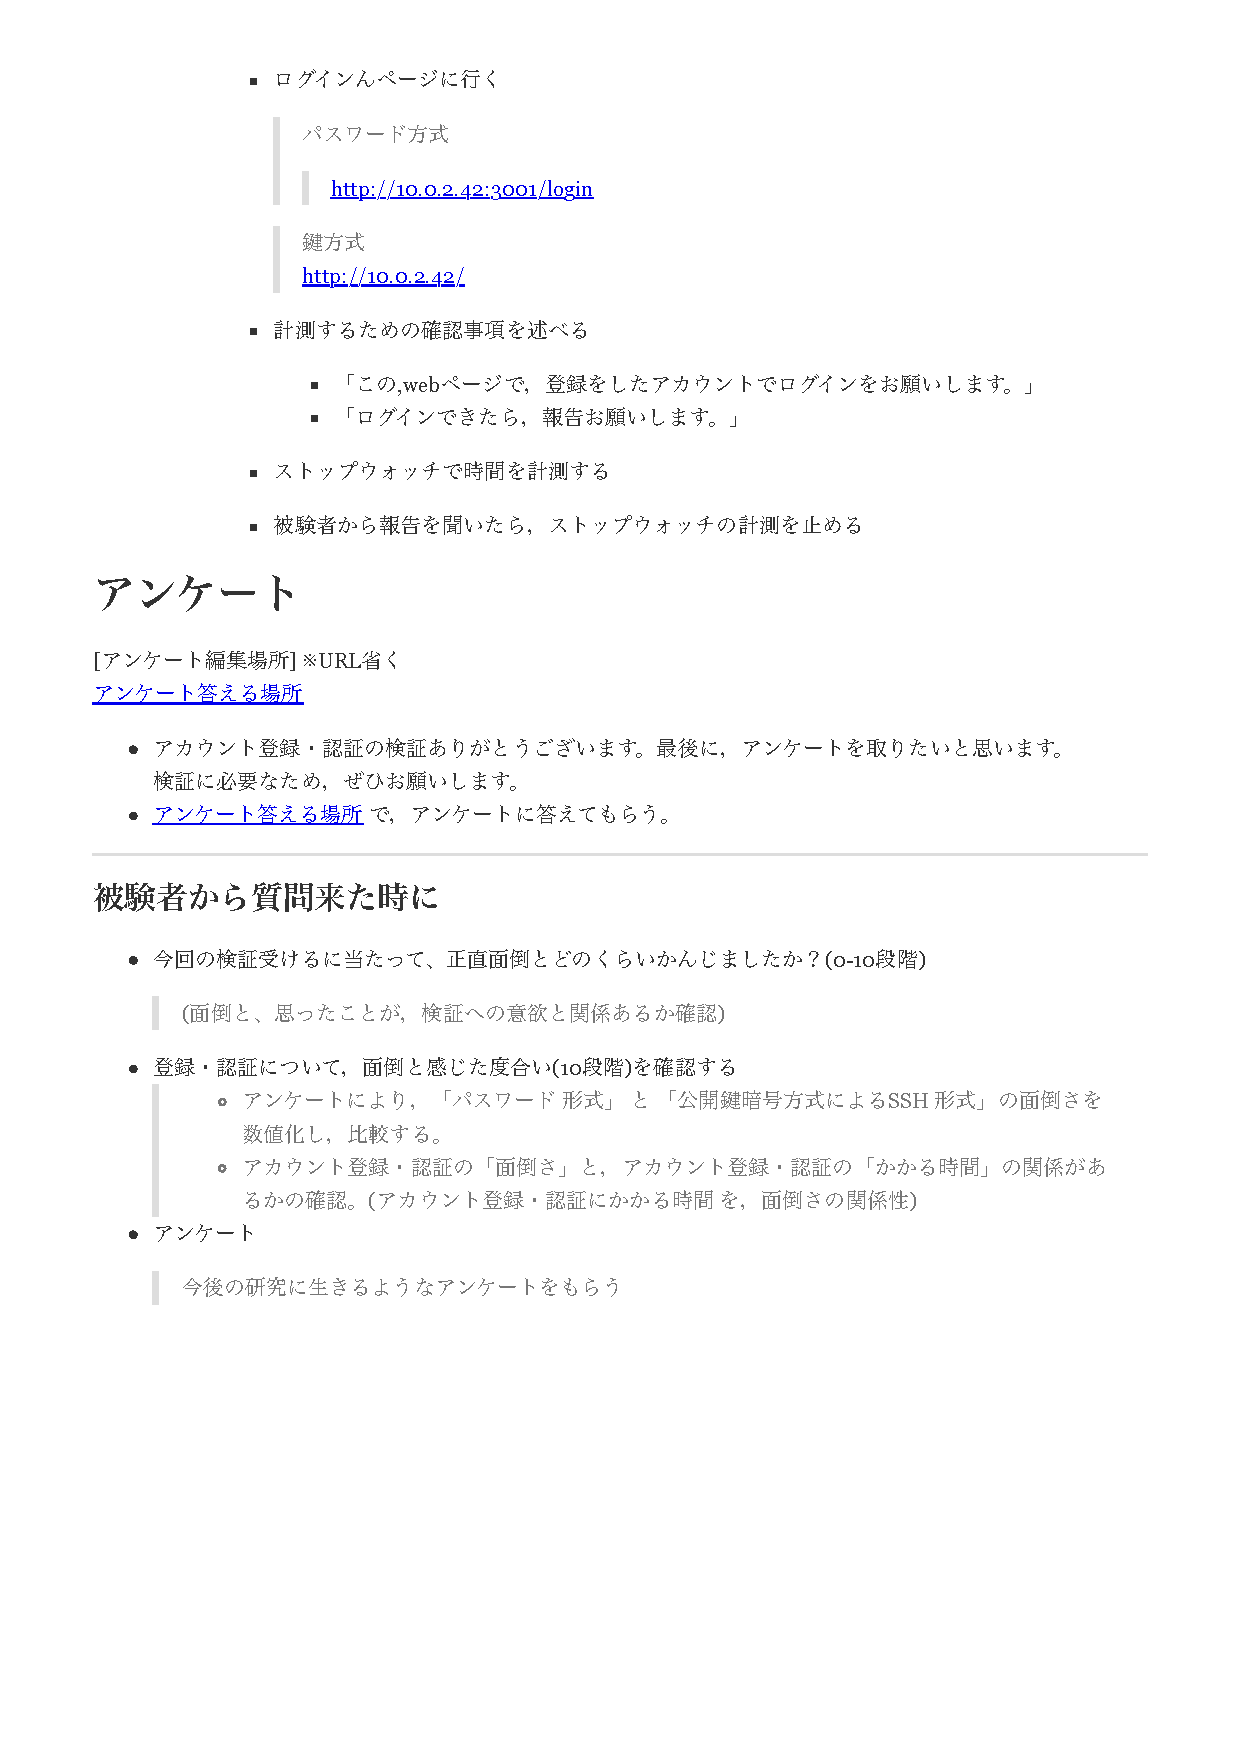
\includegraphics[width=15cm]{./fig/chapter4/inspect_1/manual/manual_2.pdf}
     \caption{検証マニュアル2}
     \label{検証マニュアル2}
 \end{figure}

 \subsection{検証結果}

    \subsubsection{被験者について}
    \begin{itemize}
        \item 琉球大学情報工学科の学生(4人)
    \end{itemize}


    \subsubsection{時間の観点からの面倒さ}
        ここでは被験者に行ってもらった,登録・認証にかかる時間を以下の表\ref{検証1 認証・登録の計測時間}に示す.
        表\ref{検証1 認証・登録の計測時間} は パスワード方式,鍵方式の登録・認証それぞれについて,個の時間,平均時間を記述した表である.
        %表の記述
        \begin{table}[htb]
            \caption{検証1\_認証・登録の計測時間}
            \label{検証1 認証・登録の計測時間}
            \begin{tabular}{|l|r|r|r|r|r|} \hline%| (ハイプ) は縦線
                %登録・認証の種類 \textbackslash 被験者 & 被験者1 & 被験者2 & 被験者3  & 被験者4 & 平均\\ \hline%\hline は横の線
                                & 被験者1 & 被験者2 & 被験者3  & 被験者4 & 平均 \\ \hline%\hline は横の線
                登録(パスワード方式) & 24.88 & 38.99 & 28.21 & 18.04 & 27.53 \\ \hline
                認証(パスワード方式) & 16.57 & 13.24 & 21.27 & 12.23 & 15.83 \\ \hline
                登録(鍵方式)       & 19.96 & 19.14 & 21.73 & 7.81 & 17.16 \\ \hline
                認証(鍵方式)       & 14.86 & 18.63 & 18.35 & 11.47 & 15.83 \\ \hline

                %----- 最終ページの表の最下部 --------
                \multicolumn{6}{r}{\small\it (単位:秒)}\\
                \end{tabular}
        \end{table}

        %上の表の参考方法
        %%表\ref{検証1 認証・登録の計測時間}

    \subsubsection{アンケートの観点からの面倒さ}
        ここでは,被験者に対して,2つの方式の登録・認証が終わった直後に,
        記入してもらったアンケートについての数値のまとめを以下の表\ref{検証1 アンケートによる6段階評価}に示す.
        表\ref{検証1 アンケートによる6段階評価}は 被験者による パスワード方式,鍵方式の登録・認証それぞれについて0 〜 5 段階評価,さらに,検証自体の面倒さについての評価を加えて まとめた表である.
        %表の記述
        \begin{table}[htb]
            \caption{検証1\_アンケートによる6段階評価}
            \label{検証1 アンケートによる6段階評価}
            \begin{tabular}{|l|r|r|r|r|r|} \hline%| (ハイプ) は縦線
                %登録・認証の種類 \textbackslash 被験者 & 被験者1 & 被験者2 & 被験者3  & 被験者4 & 平均\\ \hline%\hline は横の線
                                        & 被験者1 & 被験者2 & 被験者3  & 被験者4 & 平均 \\ \hline%\hline は横の線
                登録(パスワード方式)の面倒さ & 1 & 1 & 2 & 0 & 1 \\ \hline
                認証(パスワード方式)の面倒さ & 1 & 1 & 2 & 1 & 1.25 \\ \hline
                登録(鍵方式)の面倒さ       & 0 & 2 & 0 & 1 & 0.75 \\ \hline
                認証(鍵方式)の面倒さ       & 0 & 2 & 0 & 2 & 1 \\ \hline
                検証自体の面倒さ       & 2 & 1 & 1 & 1 & 1.25 \\ \hline
    
                %----- 最終ページの表の最下部 --------
                \multicolumn{6}{r}{\small\it (0 〜 5段階)}\\
            \end{tabular}
        \end{table}

        %上の表の参考方法
        %%表\ref{検証1 アンケートによる6段階評価}

 \newpage


 \subsection{考察}
 時間の観点での"面倒さ"では,時間がかかる方"面倒"と感じると予測していたため,
 パスワードの観点と,アンケートの観点の面倒さの数値は比例すると考えていた。
 しかし,表\ref{検証1 認証・登録の計測時間},表\ref{検証1 アンケートによる6段階評価} 被験者2の
 パスワード方式と鍵方式の「アカウント登録・認証にかかる時間の大きさ」と,
 「アンケートによる面倒の数値」が,半比例関係だった.
 上記のような結果になった理由としては2通り考えられる.
 1つ目は,普段登録,認証で使っている,パスワード方式の方が,慣れているため,「面倒」と感じにくかったと考察することができる.
 2つ目は,アンケートに「PCから秘密鍵を選択するのが少し面倒だと感じた。」とあり,鍵の管理を面倒だと感じたことが,影響したと思われる.

 鍵方式についてのアンケートの結果に「なんかわかった」というアンケートの記述があった.
 被験者に確認したところ,鍵方式の登録・認証の流れがよく分からなかったとのことだった.
 実際に,鍵方式で登録する際に,登録できたのか戸惑っていた。
 この原因としては,鍵方式の登録・認証の流れが分からなかったためだと考えられる.

 表\ref{検証1 アンケートによる6段階評価}の検証自体の面倒さは0数値にする人が無く,
 検証自体に,少しながら面倒と感じていることが分かる.
 その原因としては,検証するためのWEBページ(図\ref{検証1アカウント作成(パスワード方式)} 〜 図\ref{検証1認証成功後(鍵方式)} )が
 デバッグページのままで,登録・認証が作業的になってしまったためだと考えられる.

 検証後の聞き取りで,パスワード方式の登録で以下のような日常的に,
 使用しないと思われるパスワードの確認ができた.
 \begin{itemize}
    \item パスワードの使い回し
    \item パスワード "password"を設定する
 \end{itemize}
 そのことから,検証方法のマニュアルに,
 普段使うようなWEBサービスのように実施してもらうような注意事項を用意する必要がある.

\newpage





%% 検証2でやるやつ
%\section{検証2}
%  \subsection{検証背景}
%    \subsubsection{検証目的}
%    \subsubsection{検証手段} 
%  \subsection{検証環境}                        OK
%    \subsubsection{検証場所}                   OK
%    \subsubsection{検証の流れ}                 OK
%    \subsubsection{検証画面}                   OK
%    \subsubsection{検証マニュアル}              OK
%  \subsection{検証結果}
%  \subsection{考察}




\section{検証2}
  \subsection{検証背景}
    \subsubsection{検証目的}
    password認証方式の,新規登録・認証の面倒さを解決するために,第3章の提案手法で
    password認証方式に変わる,公開鍵暗号方式によるssh認証を用いた,WEBサービス認証の提案を行った。\\
    しかしながら,提案だけだと,新規登録・認証の面倒さを解決していることの根拠に乏しい。
    よって,検証を行い,第3章の提案手法は"面倒さの軽減"に効果的に繋がっているかの確認をする。
    \subsubsection{検証手段} 
    検証の手段としては,実際に,以下の2つの認証方式の登録・認証を被験者に体験してもらう。
    %また,実験マニュアルを作成し,実験者は被験者に対して,同じように接するようにする。

    \begin{itemize}
    \item パスワード方式認証(以後 "パスワード認証"と記述する)
    \item 公開鍵暗号暗号方式によるssh認証(以後 "鍵認証”と記述する)
    \end{itemize}

    その後,2つの観点から,"面倒さ"を数値化する。
    1つ目の観点は「時間」である。
    "面倒さ"をアカウント登録・認証にかかる時間と推測し,計測化する。
    詳しい詳細については,検証環境のマニュアルに記述する。
    %まず,パスワード 形式による登録・認証の時間計測をそれぞれ行う。
    % 次に,公開鍵暗号方式によるSSH 形式登録・認証の時間計測をそれぞれ行う。
    % 最後に,上記の形式による時間計測を比較する。
    2つ目の観点は「アンケート」である。
    アンケートには,点数で答える方式,文字で記入する欄 の2つがあり,点数で答える方式により"面倒さ”を数値化する。
    アンケートの細かい内容は,4.1.3の検証画面に記述する。

    また,アンケートには"面倒さ"を数値化する以外にも,以下の2つの意味を込める。
    1つ目の意味は次の通りである。
    アカウント登録・認証にかかる時間 を,"面倒さ"と予想して検証しているが,その予想を確かめる必要がある。
    アンケートを取ることにより,「アカウント登録・認証にかかる時間」と,「アンケートによる面倒さ」が比例していることを確認することで,予想を確かめることができる。
    また,被験者の状態も確認することで,面倒と感じるのが,検証自体に対しての面倒さと関係があるのかを確認する。
    2つ目の意味は次のとおりである。
    記入欄で,改善点や感じたことの意見をもらうことで,今後の研究に生きるようなアンケートをもらう。

    検証1より効果的な検証方法にするため変更して検証をおこなう.変更点とその理由についてはそれぞれの項で述べる.

  \newpage

  \subsection{検証環境} 
    \subsubsection{検証場所}% 基本一緒?
       第3章で記述したとおり,検証場所は学科のVMを用いているため,学科のネットワーク内(有線LAN,wifiアクセスポイント{ie-ryukyu})
        から,アクセスして検証を行う。
    \subsubsection{検証の流れ}% 基本一緒?
        ここでは,被験者に行ってもらう,検証の流れを記述する。
        時間の観点で"面倒さ"を数値化する検証では,被験者にはパスワード方式,鍵方式の登録・認証をそれぞれ行ってもらう。その時,被験者は時間を測る。 
        また,再現性を持って,検証を行うためにマニュアルを作成し,マニュアル通りに検証を行う。
        アンケートの観点で"面倒さ"を数値化する検証では,
        時間の観点で"面倒さ"を数値化する検証 が終わった直後に行うようにすることで,被験者の思った感情とアンケート結果の差異が少なくなるようにする。


    \newpage

    \subsubsection{検証画面}

    ここでは,検証1より効果的に検証結果目的を達成するために,修正した検証2の検証画面とその意図について述べる。

    %ここで,検証を行った際に,検証1と比較して被験者が視覚的・聴覚的に差異が生じる主な変更点を以下に述べる。

    まずは検証画面図の説明をする。\\
    パスワード方式について
    \begin{itemize}
        \item 図\ref{検証2ホーム画面(パスワード方式)}は,ホーム画面である.
        \item 図\ref{検証2アカウント作成(パスワード方式)}は,アカウント登録画面である。
        \item 図\ref{検証2認証(パスワード方式)}は,図\ref{検証2アカウント作成(パスワード方式)}で登録したアカウントに認証するための画面である。
        \item 図\ref{検証2認証成功後(パスワード方式)}は,図\ref{検証2認証(パスワード方式)}で認証成功した後の画面である。
    \end{itemize}
    %
    鍵方式について\\
    \begin{itemize}
        \item 図\ref{検証2ホーム画面(鍵方式)}は,ホーム画面である.
        \item 図\ref{検証2アカウント作成(鍵方式)}は,アカウント登録画面である。
        \item 図\ref{検証2認証(鍵方式)}は,図\ref{検証2アカウント作成(鍵方式)}で登録したアカウントに認証するための画面である。
        \item 図\ref{検証2認証成功後(鍵方式)}は,図\ref{検証2認証(鍵方式)}で認証成功した後の画面である。
    \end{itemize}



    % 言いたいやつ----------------------------------------------------------------------------------------------

    %% web画面面 -----------------------------------------------------
    %%% アンケートの"検証自体面倒"という観点から
    %%%%検証1のアンケートで,"検証自体が面倒"と答える被験者の平均が,5段階中の1であった。その原因として,
    %%%%デバッグ画面や,登録フォーム・認証フォームだけのWEB画面が,
    %%%%作業的な検証に繋がり,”検証自体が面倒"に繋がった大きな要因の一つと考えられる。
    %%%%よって,ホーム画面(図???)の用意や,デバッグの消去(図???),さらには,「幸せになれるWEBサイト」と認識してもらうことで,被験者にとって,作業的な検証から,WEBサービスに登録する検証を狙って,変更した。
    %% web画面面 -----------------------------------------------------

    %% 細かいやつ
    %%%アンケートは検証1と同じ質問(意図)をしているため,割愛する。

    % 言いたいやつ----------------------------------------------------------------------------------------------

    次に,検証1 との変更点と,その意図について述べる。
    %アンケートの"検証自体面倒"という観点から
    検証1のアンケート(図\ref{検証2アカウント作成(鍵方式)})で,"検証自体が面倒"と答える被験者の平均が,5段階中の1であった。その原因として,
    デバッグ画面や,登録フォーム・認証フォームだけのWEB画面が,
    作業的な検証に繋がり,"検証自体が面倒"に繋がった大きな要因の一つと考えられる。
    よって,ホーム画面(図\ref{検証2ホーム画面(パスワード方式)},図\ref{検証2ホーム画面(鍵方式)})の用意や,
    デバッグのための文字の消去(図\ref{検証2アカウント作成(パスワード方式)} 〜 図\ref{検証2認証成功後(パスワード方式)} , \ref{検証2アカウント作成(鍵方式)} 〜 \ref{検証2アカウント作成(鍵方式)}),
    さらには,「幸せになれるWEBサイト」( 図\ref{検証2ホーム画面(パスワード方式)} 〜 \ref{検証2アカウント作成(鍵方式)} )と認識してもらうことで,
    被験者にとって,作業的な検証から,WEBサービスに登録する検証になることを狙って,変更した。









    % パスワード方式のスクショ---------------------------
    \vspace{4cm}%図の位置を正しくする!
    %\begin{figure}[h]
    \begin{figure}[H]
        %\centering
        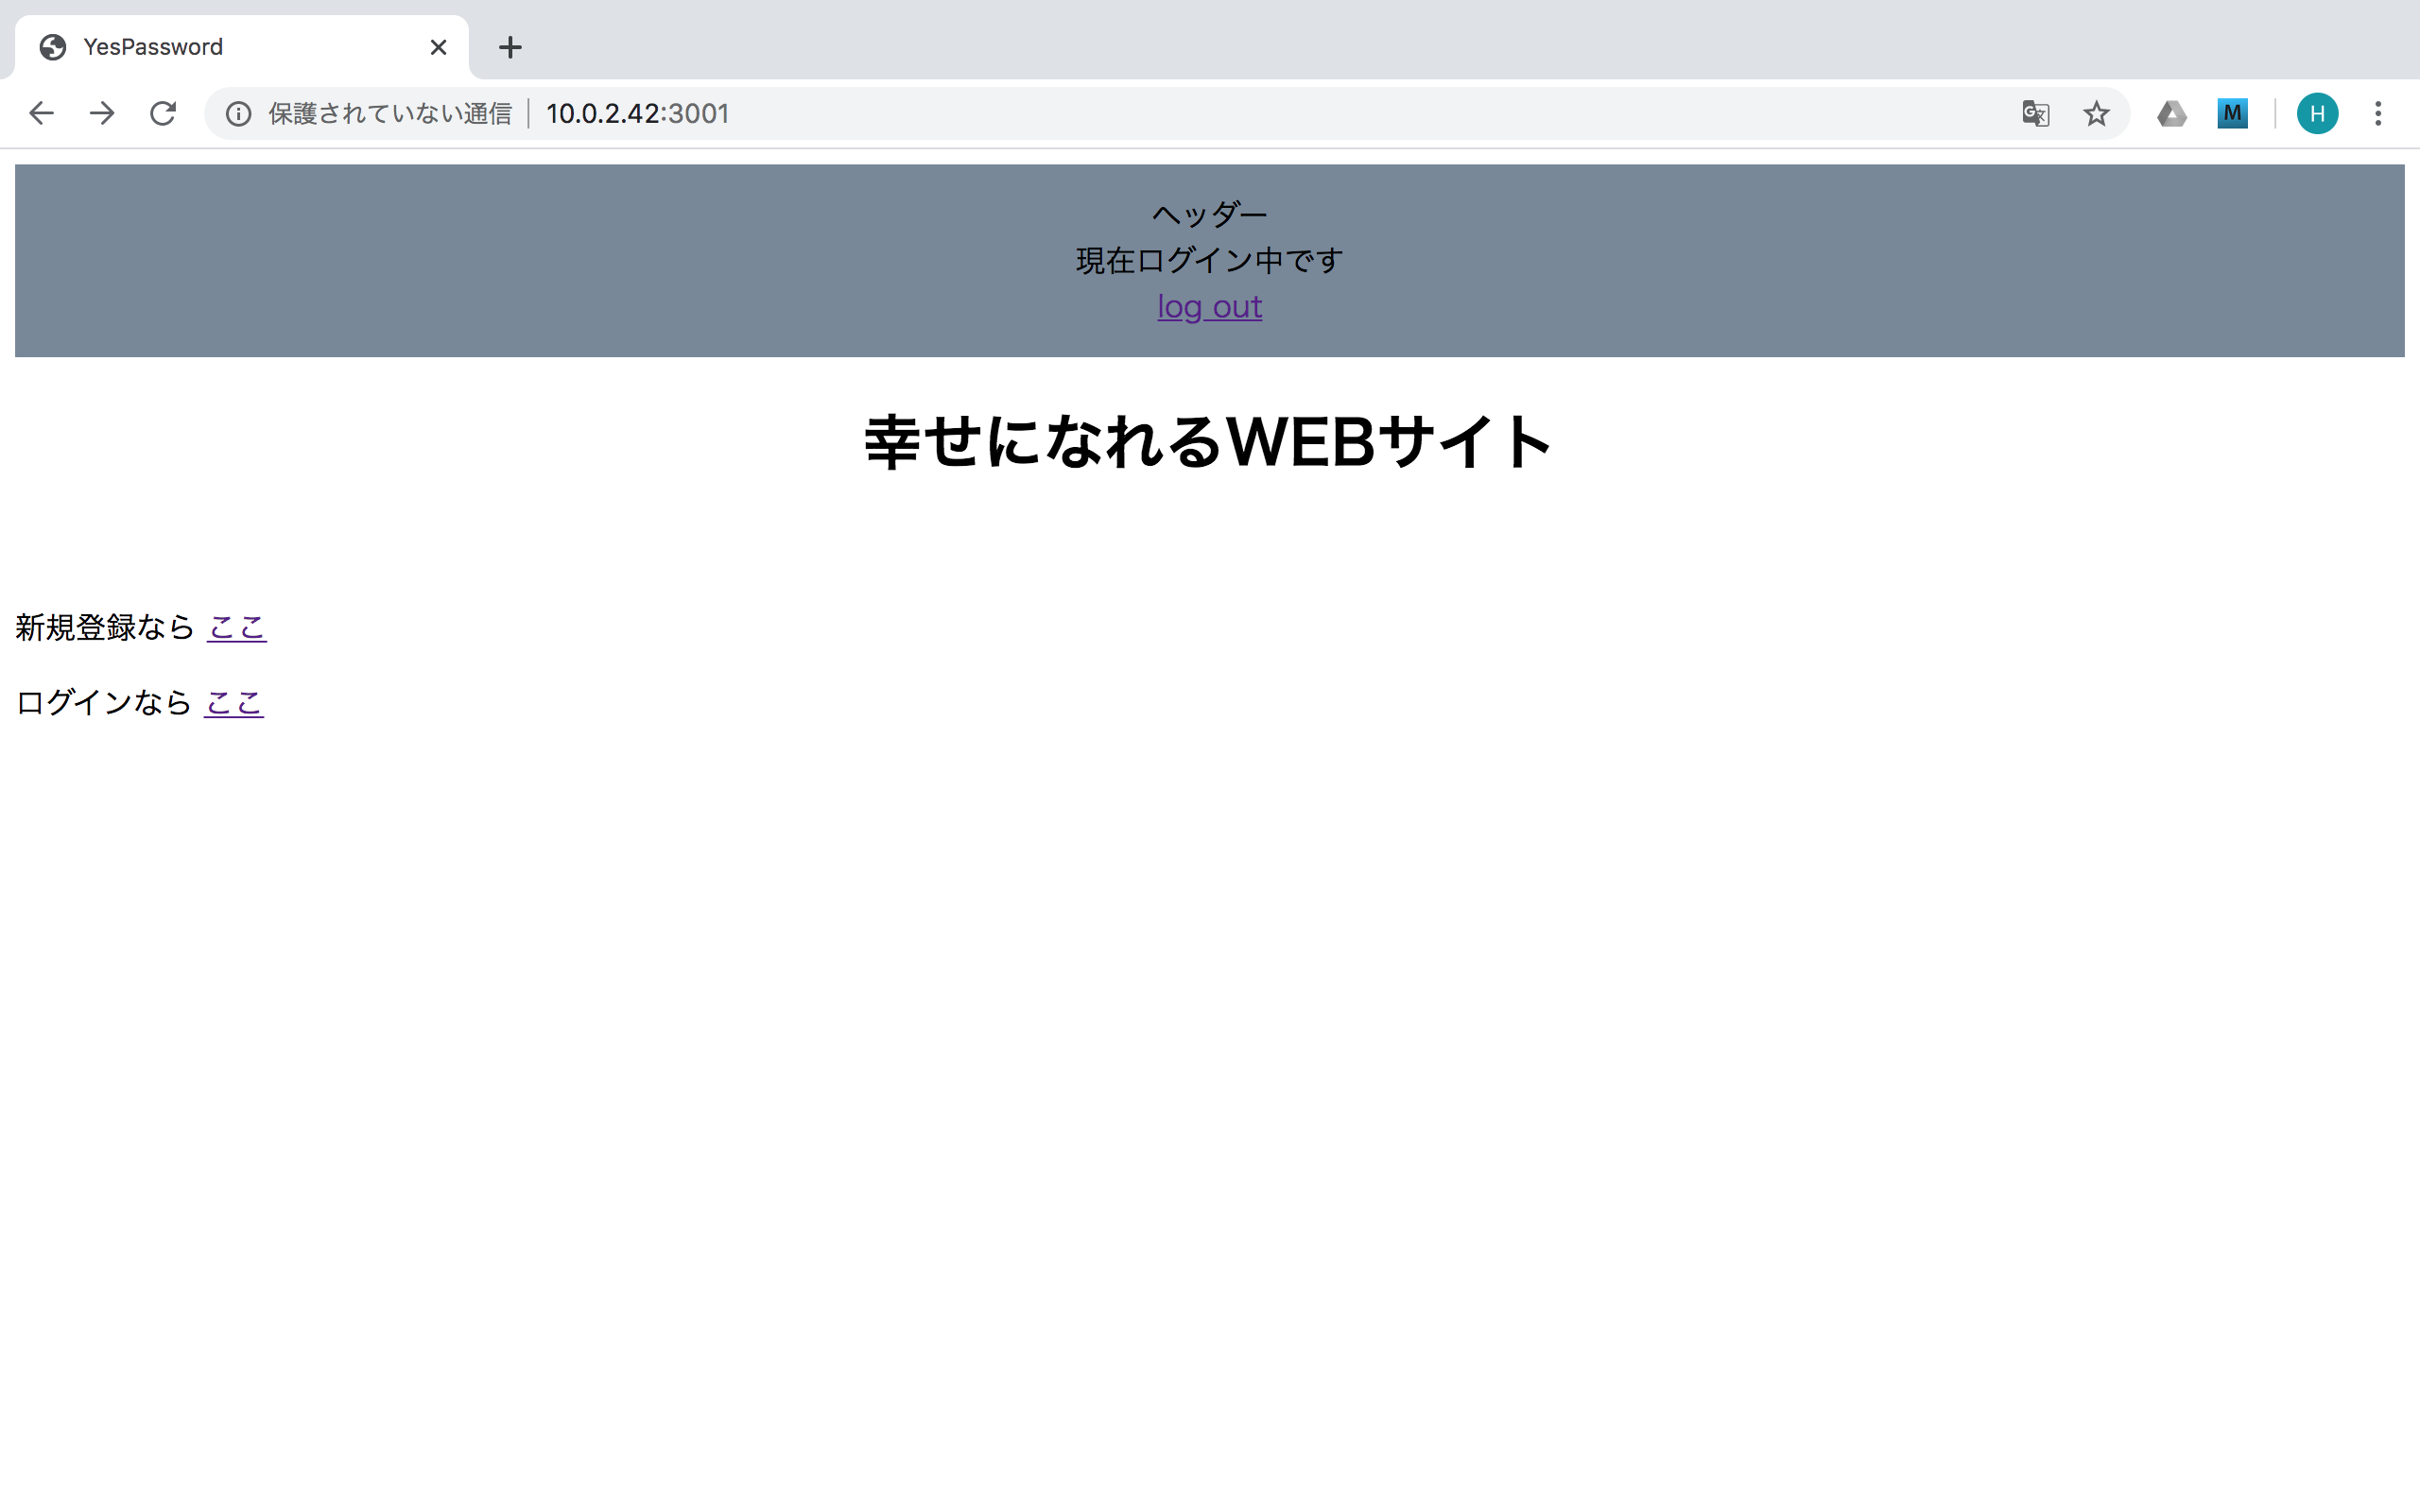
\includegraphics[height=8.4cm]{./fig/chapter4/inspect_2/password_screnn/home.png}
        \caption{検証2\_ホーム画面(パスワード方式)}
        \label{検証2ホーム画面(パスワード方式)}
    \end{figure}


    \vspace{4cm}%図の位置を正しくする!
    %\begin{figure}[h]
    \begin{figure}[H]
        %\centering
        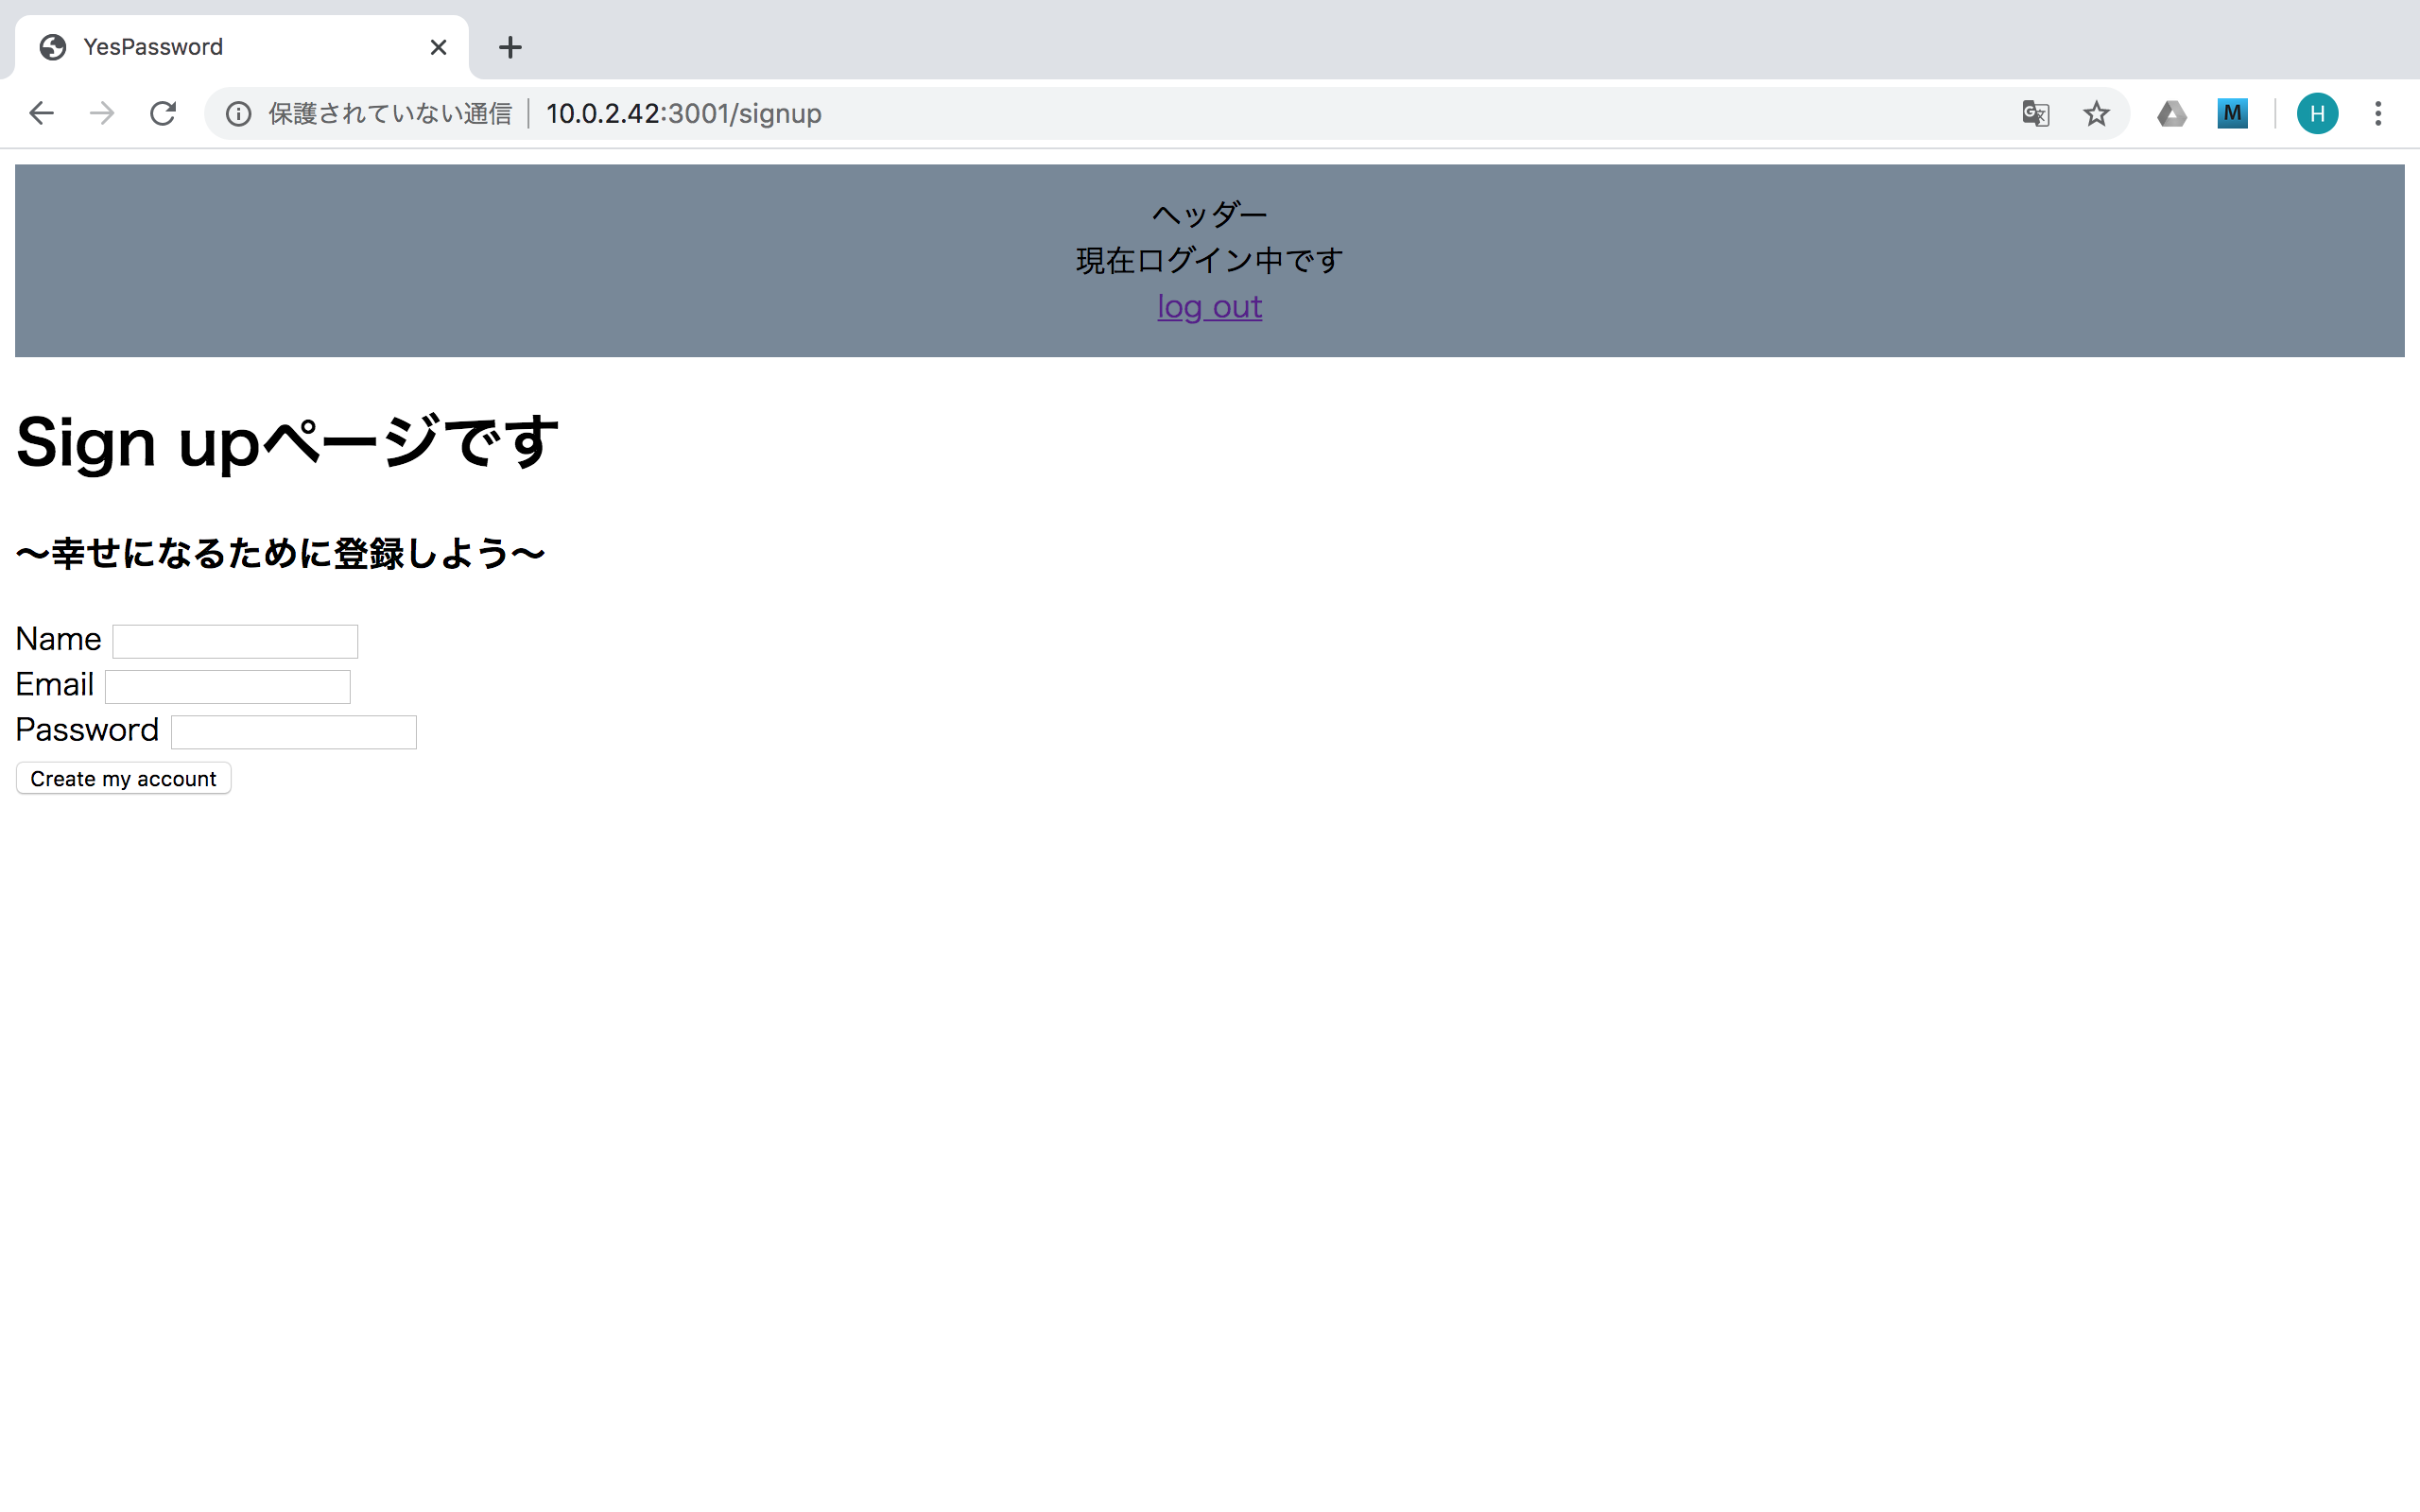
\includegraphics[height=8.4cm]{./fig/chapter4/inspect_2/password_screnn/sign_up.png}
        \caption{検証2\_アカウント作成(パスワード方式)}
        \label{検証2アカウント作成(パスワード方式)}
    \end{figure}

    \vspace{4cm}%図の位置を正しくする!
    %\begin{figure}[h]
    \begin{figure}[H]
        %\centering
        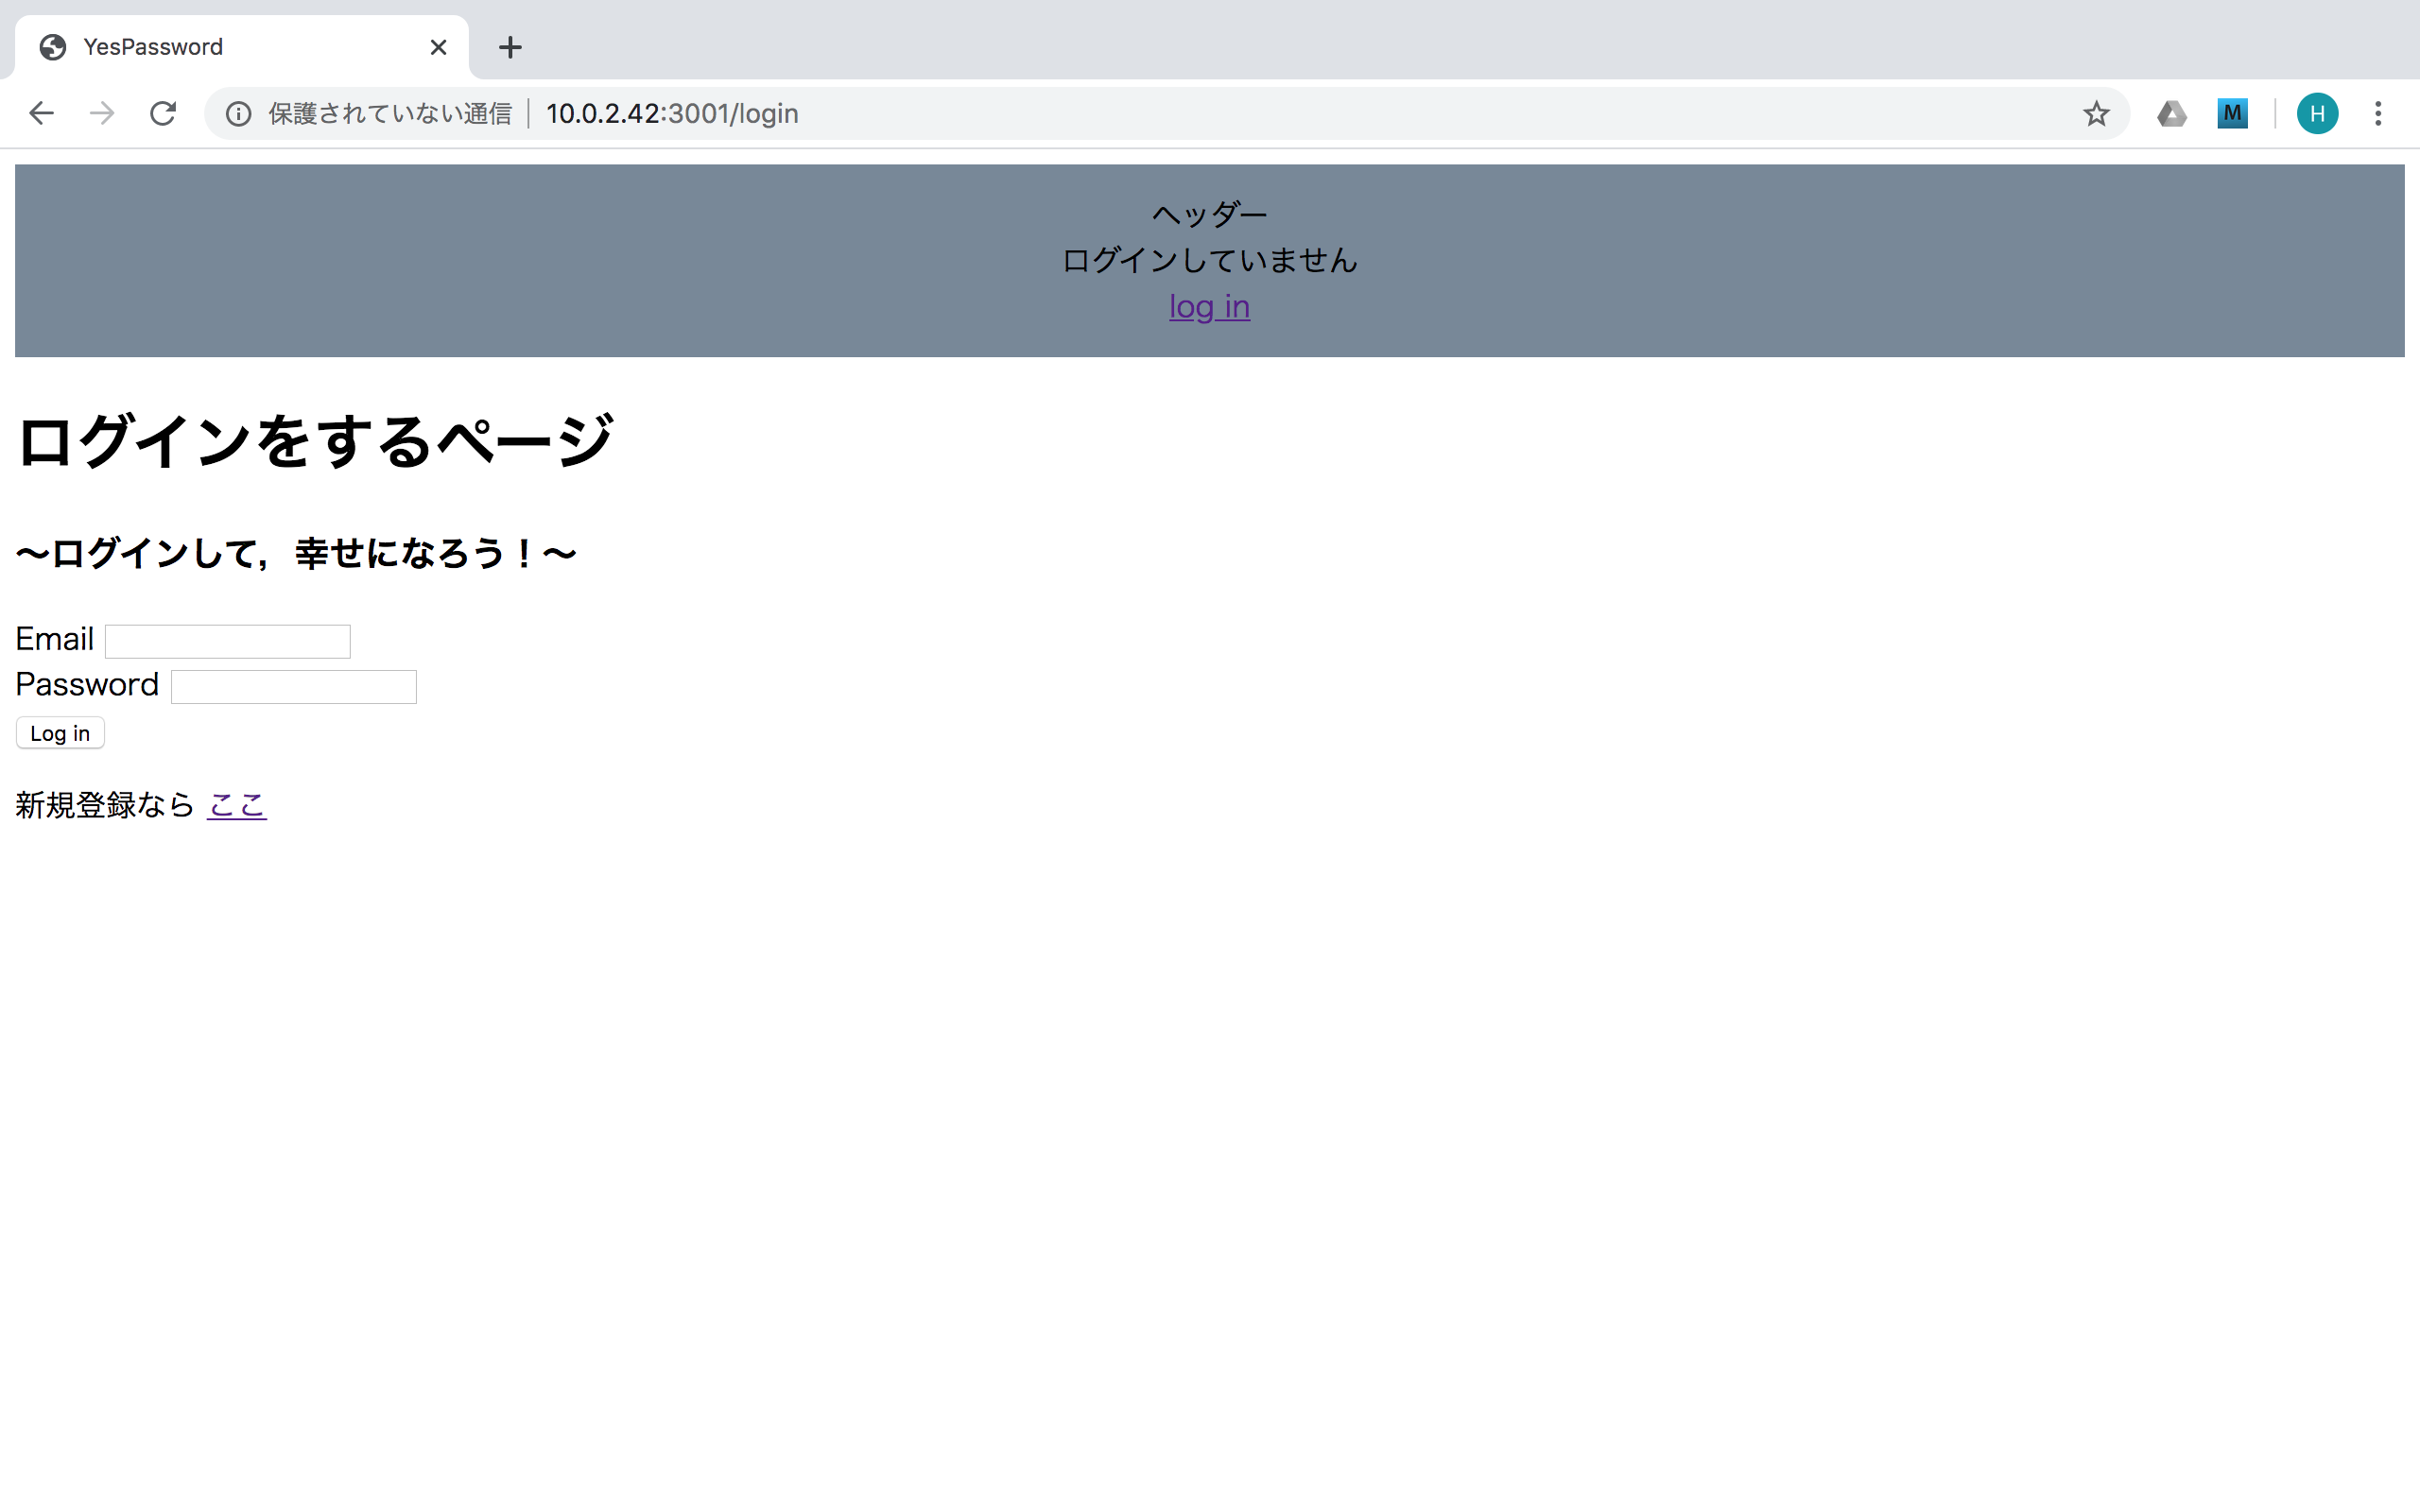
\includegraphics[height=8.4cm]{./fig/chapter4/inspect_2/password_screnn/login.png}
        \caption{検証2\_認証(パスワード方式)}
        \label{検証2認証(パスワード方式)}
    \end{figure}

    \vspace{4cm}%図の位置を正しくする!
    %\begin{figure}[h]
    \begin{figure}[H]
        %\centering
        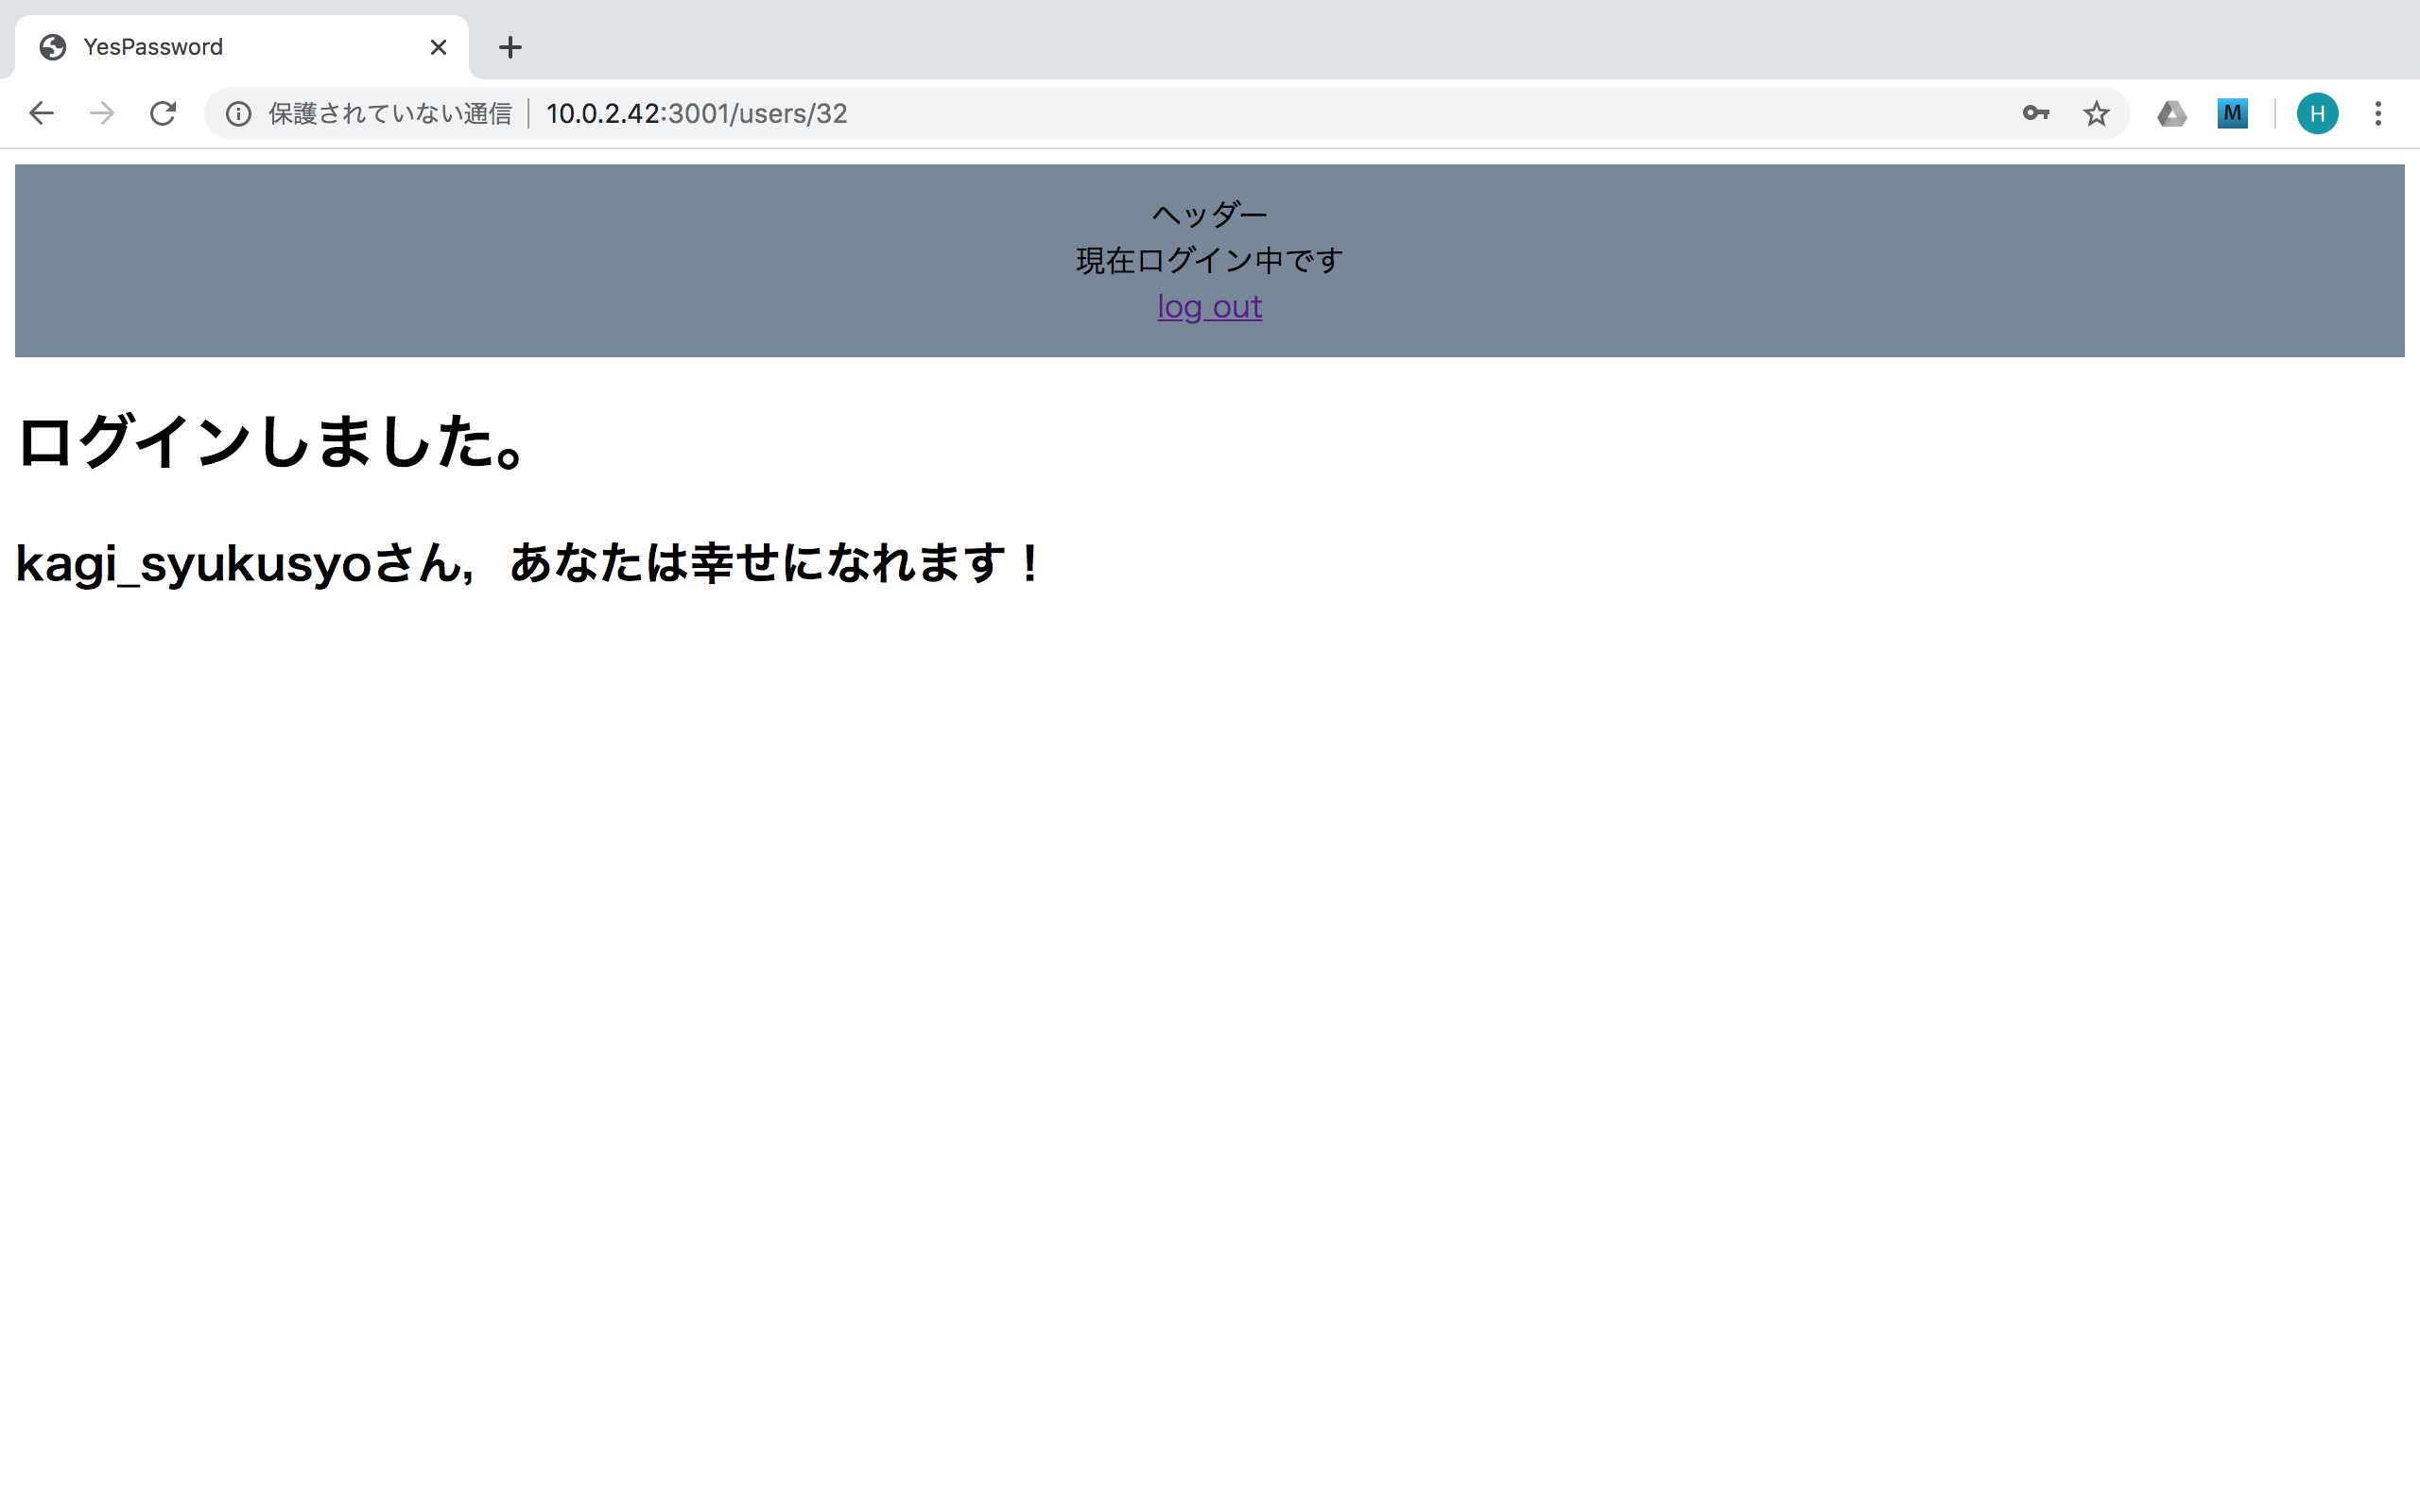
\includegraphics[height=8.4cm]{./fig/chapter4/inspect_2/password_screnn/success.png}
        \caption{検証2\_認証成功後(パスワード方式)}
        \label{検証2認証成功後(パスワード方式)}
    \end{figure}
    % パスワード方式のスクショ---------------------------

    % 鍵方式のスクショ----------------------------------
    \vspace{4cm}%図の位置を正しくする!
    \begin{figure}[H]
        %\centering
        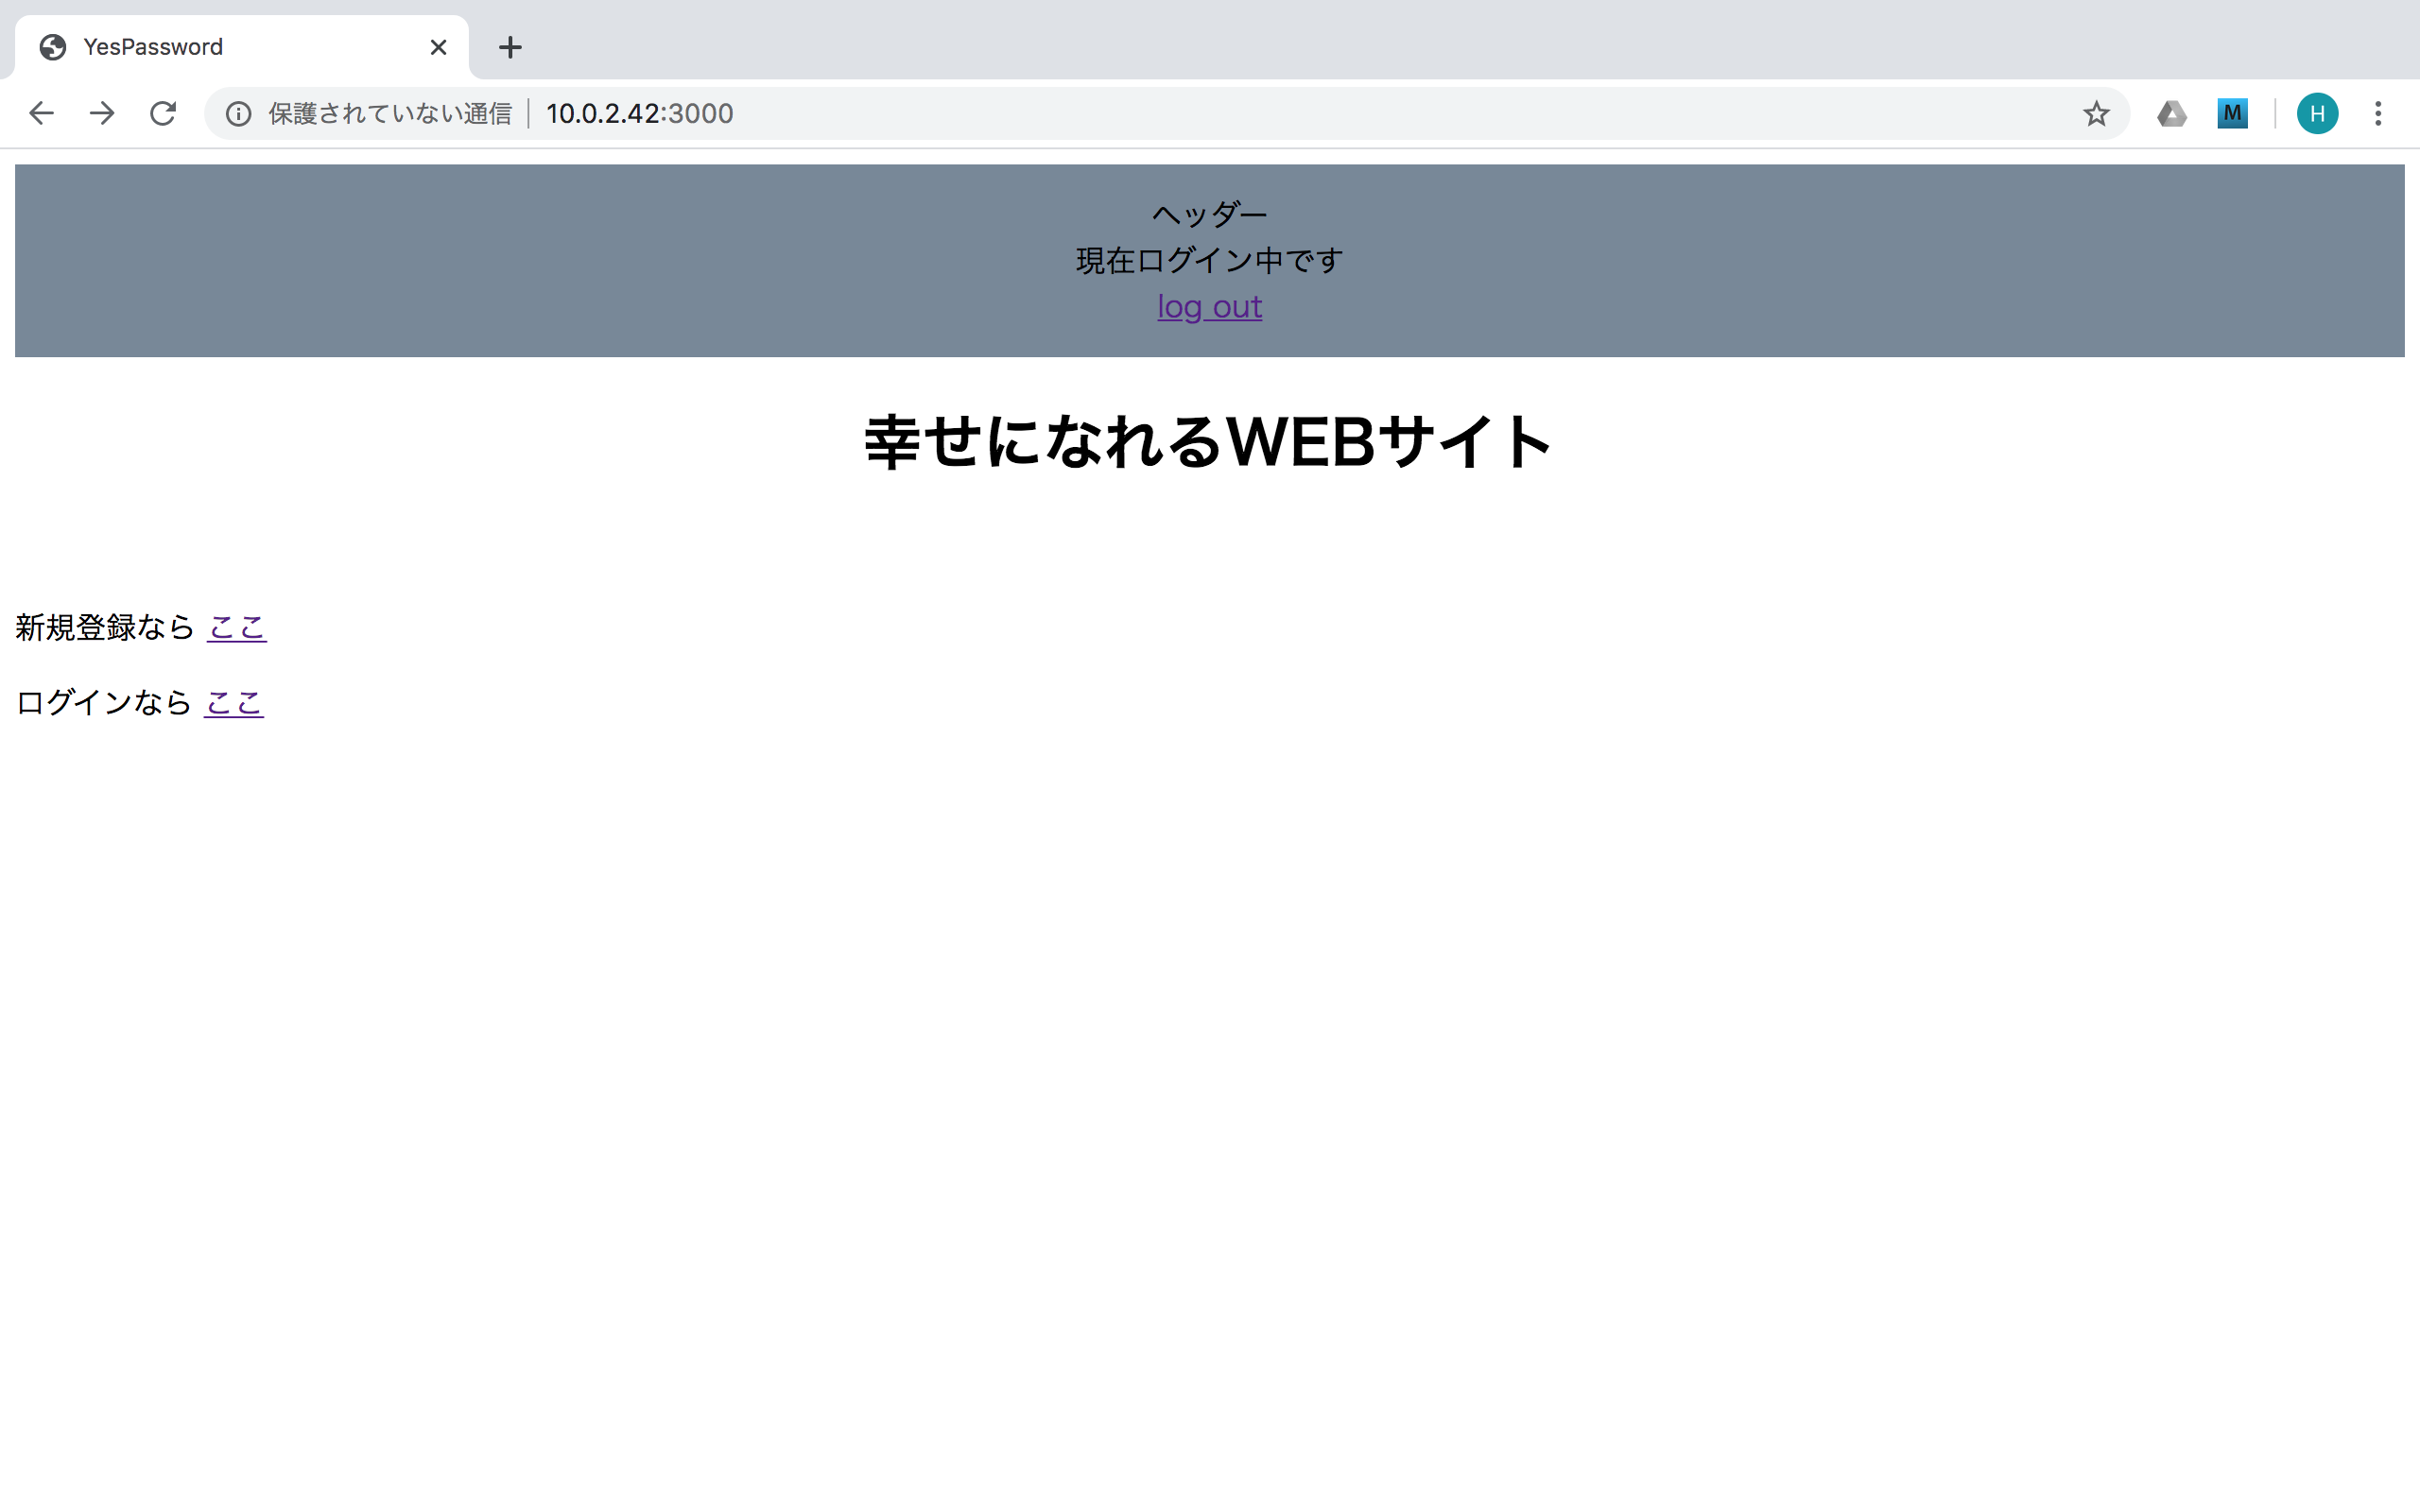
\includegraphics[height=8.4cm]{./fig/chapter4/inspect_2/key_screnn/home.png}
        \caption{検証2\_ホーム画面(鍵方式)}
        \label{検証2ホーム画面(鍵方式)}
    \end{figure}

    \vspace{4cm}%図の位置を正しくする!
    \begin{figure}[H]
        %\centering
        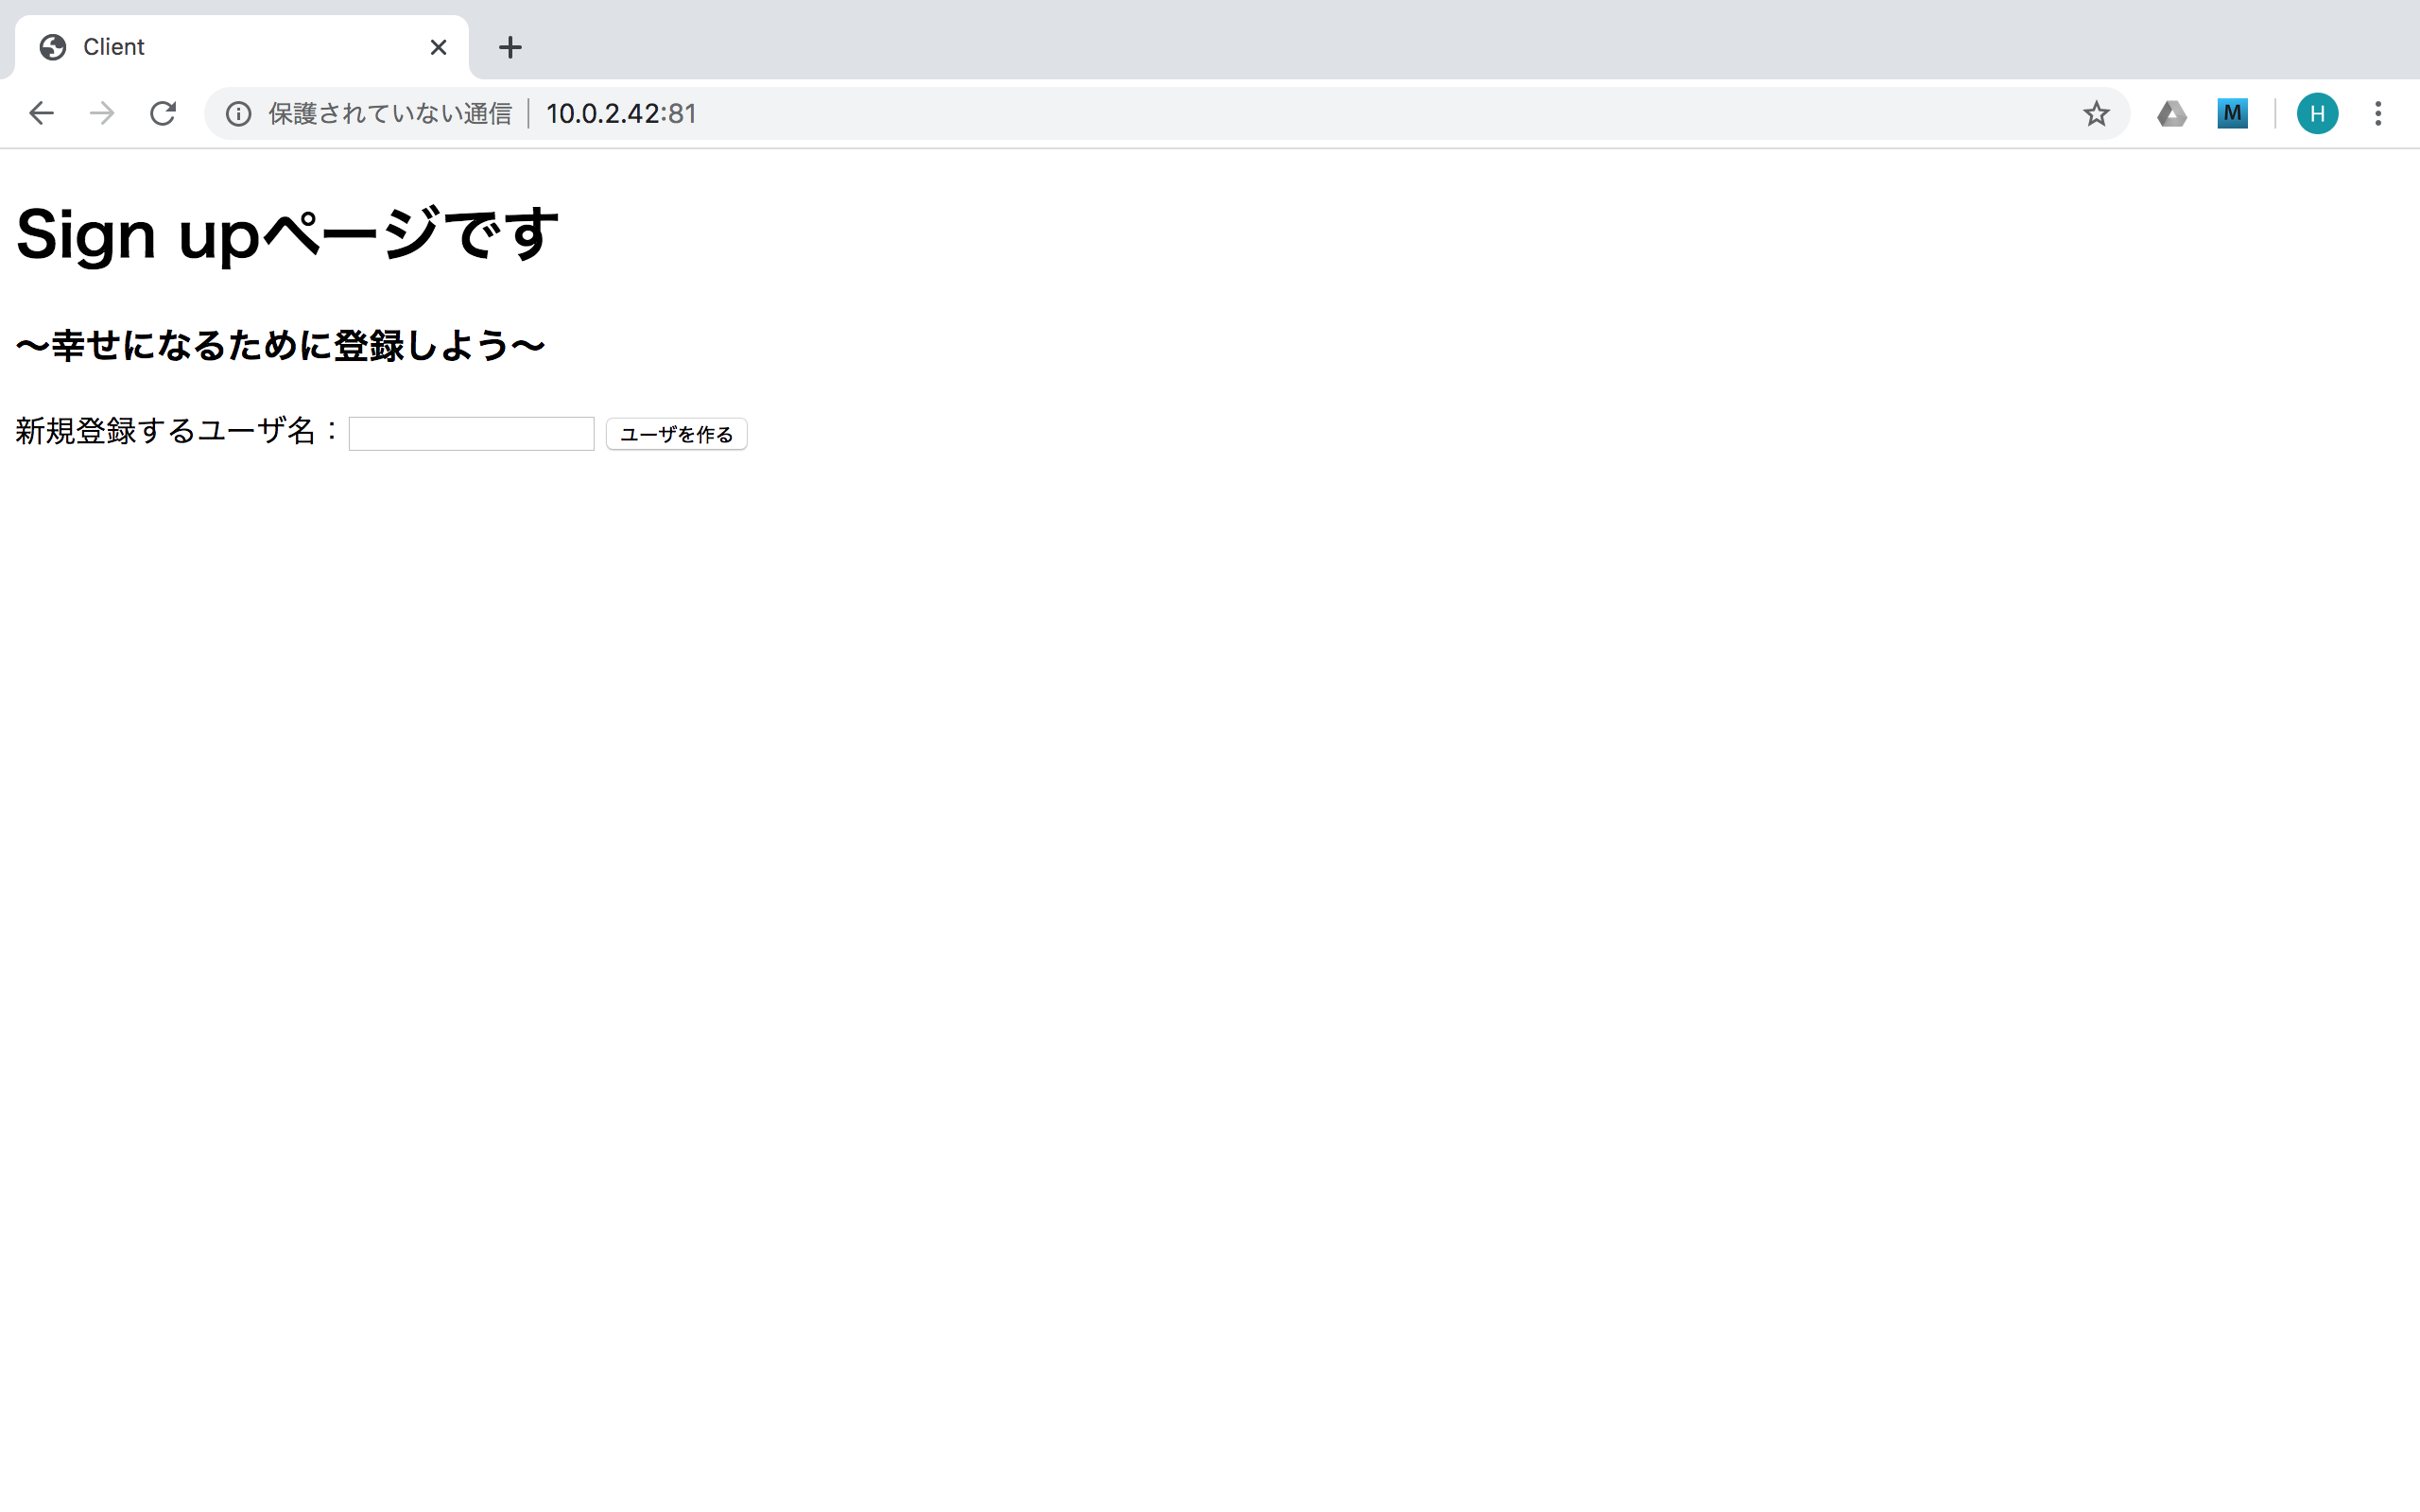
\includegraphics[height=8.4cm]{./fig/chapter4/inspect_2/key_screnn/sign_up.png}
        \caption{検証2\_アカウント作成(鍵方式)}
        \label{検証2アカウント作成(鍵方式)}
    \end{figure}

    \vspace{4cm}%図の位置を正しくする!
    \begin{figure}[H]
        %\centering
        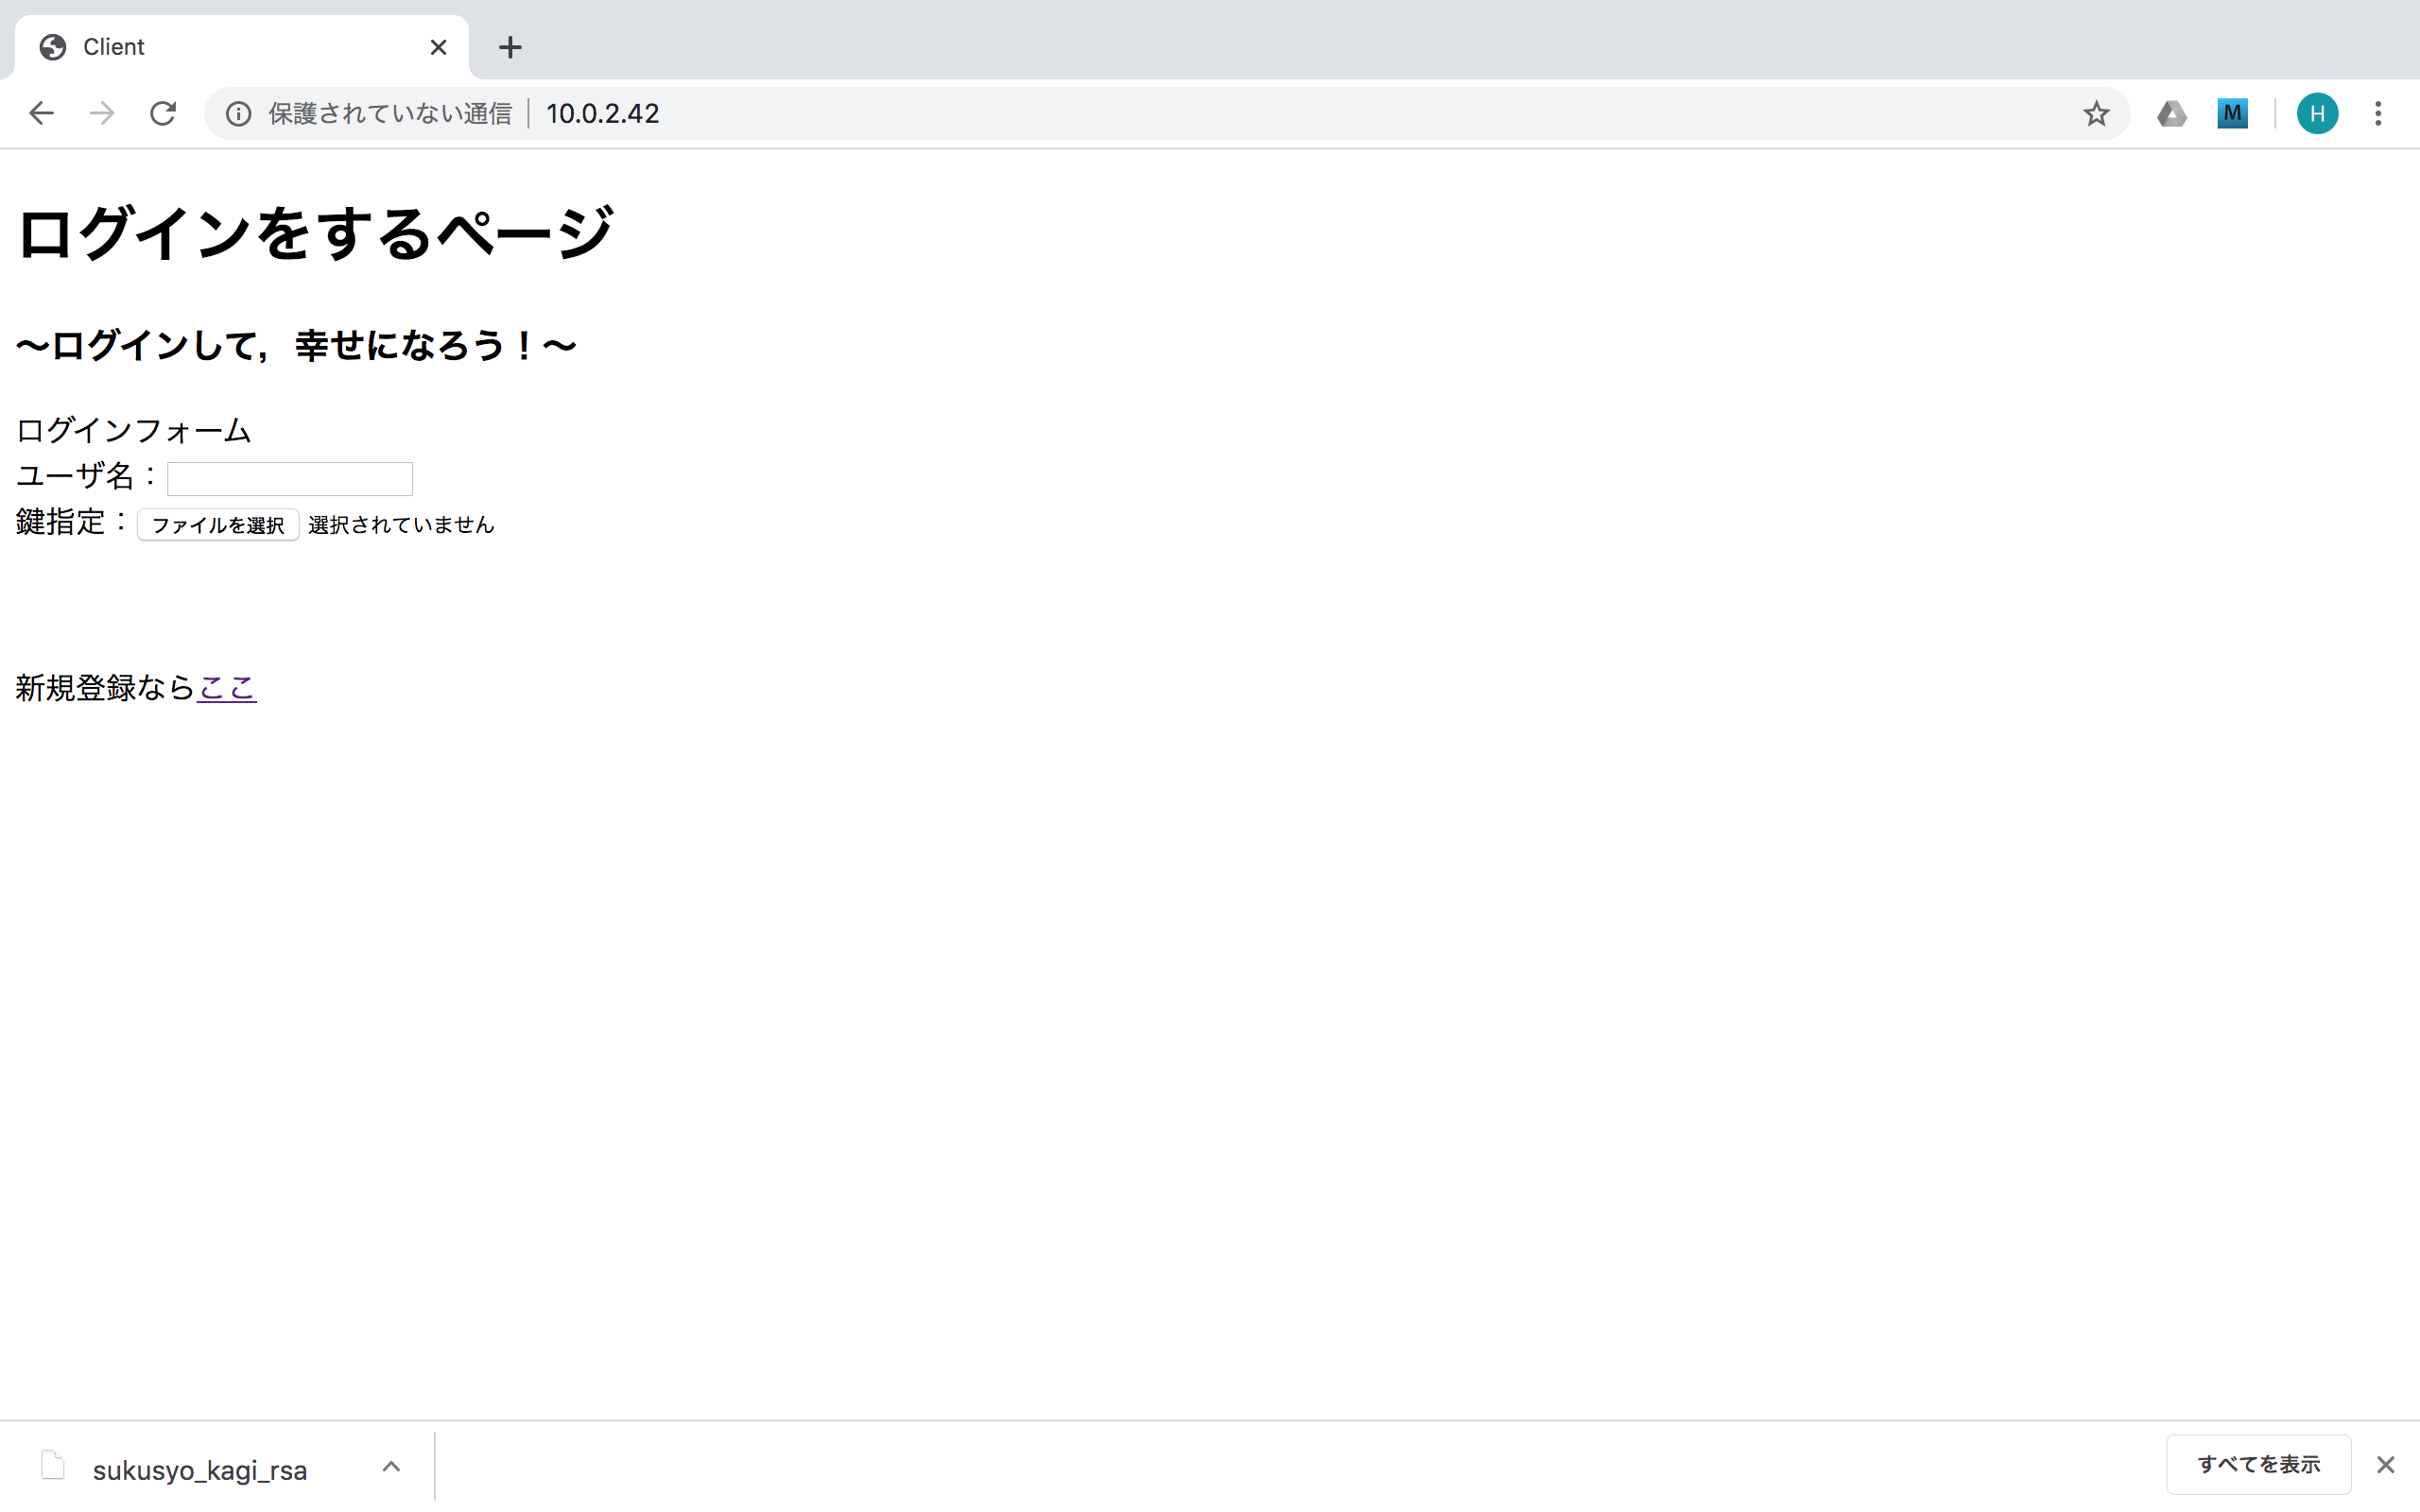
\includegraphics[height=8.4cm]{./fig/chapter4/inspect_2/key_screnn/login.png}
        \caption{検証2\_認証(鍵方式)}
        \label{検証2認証(鍵方式)}
    \end{figure}

    \vspace{4cm}%図の位置を正しくする!
    \begin{figure}[H]
        %\centering
        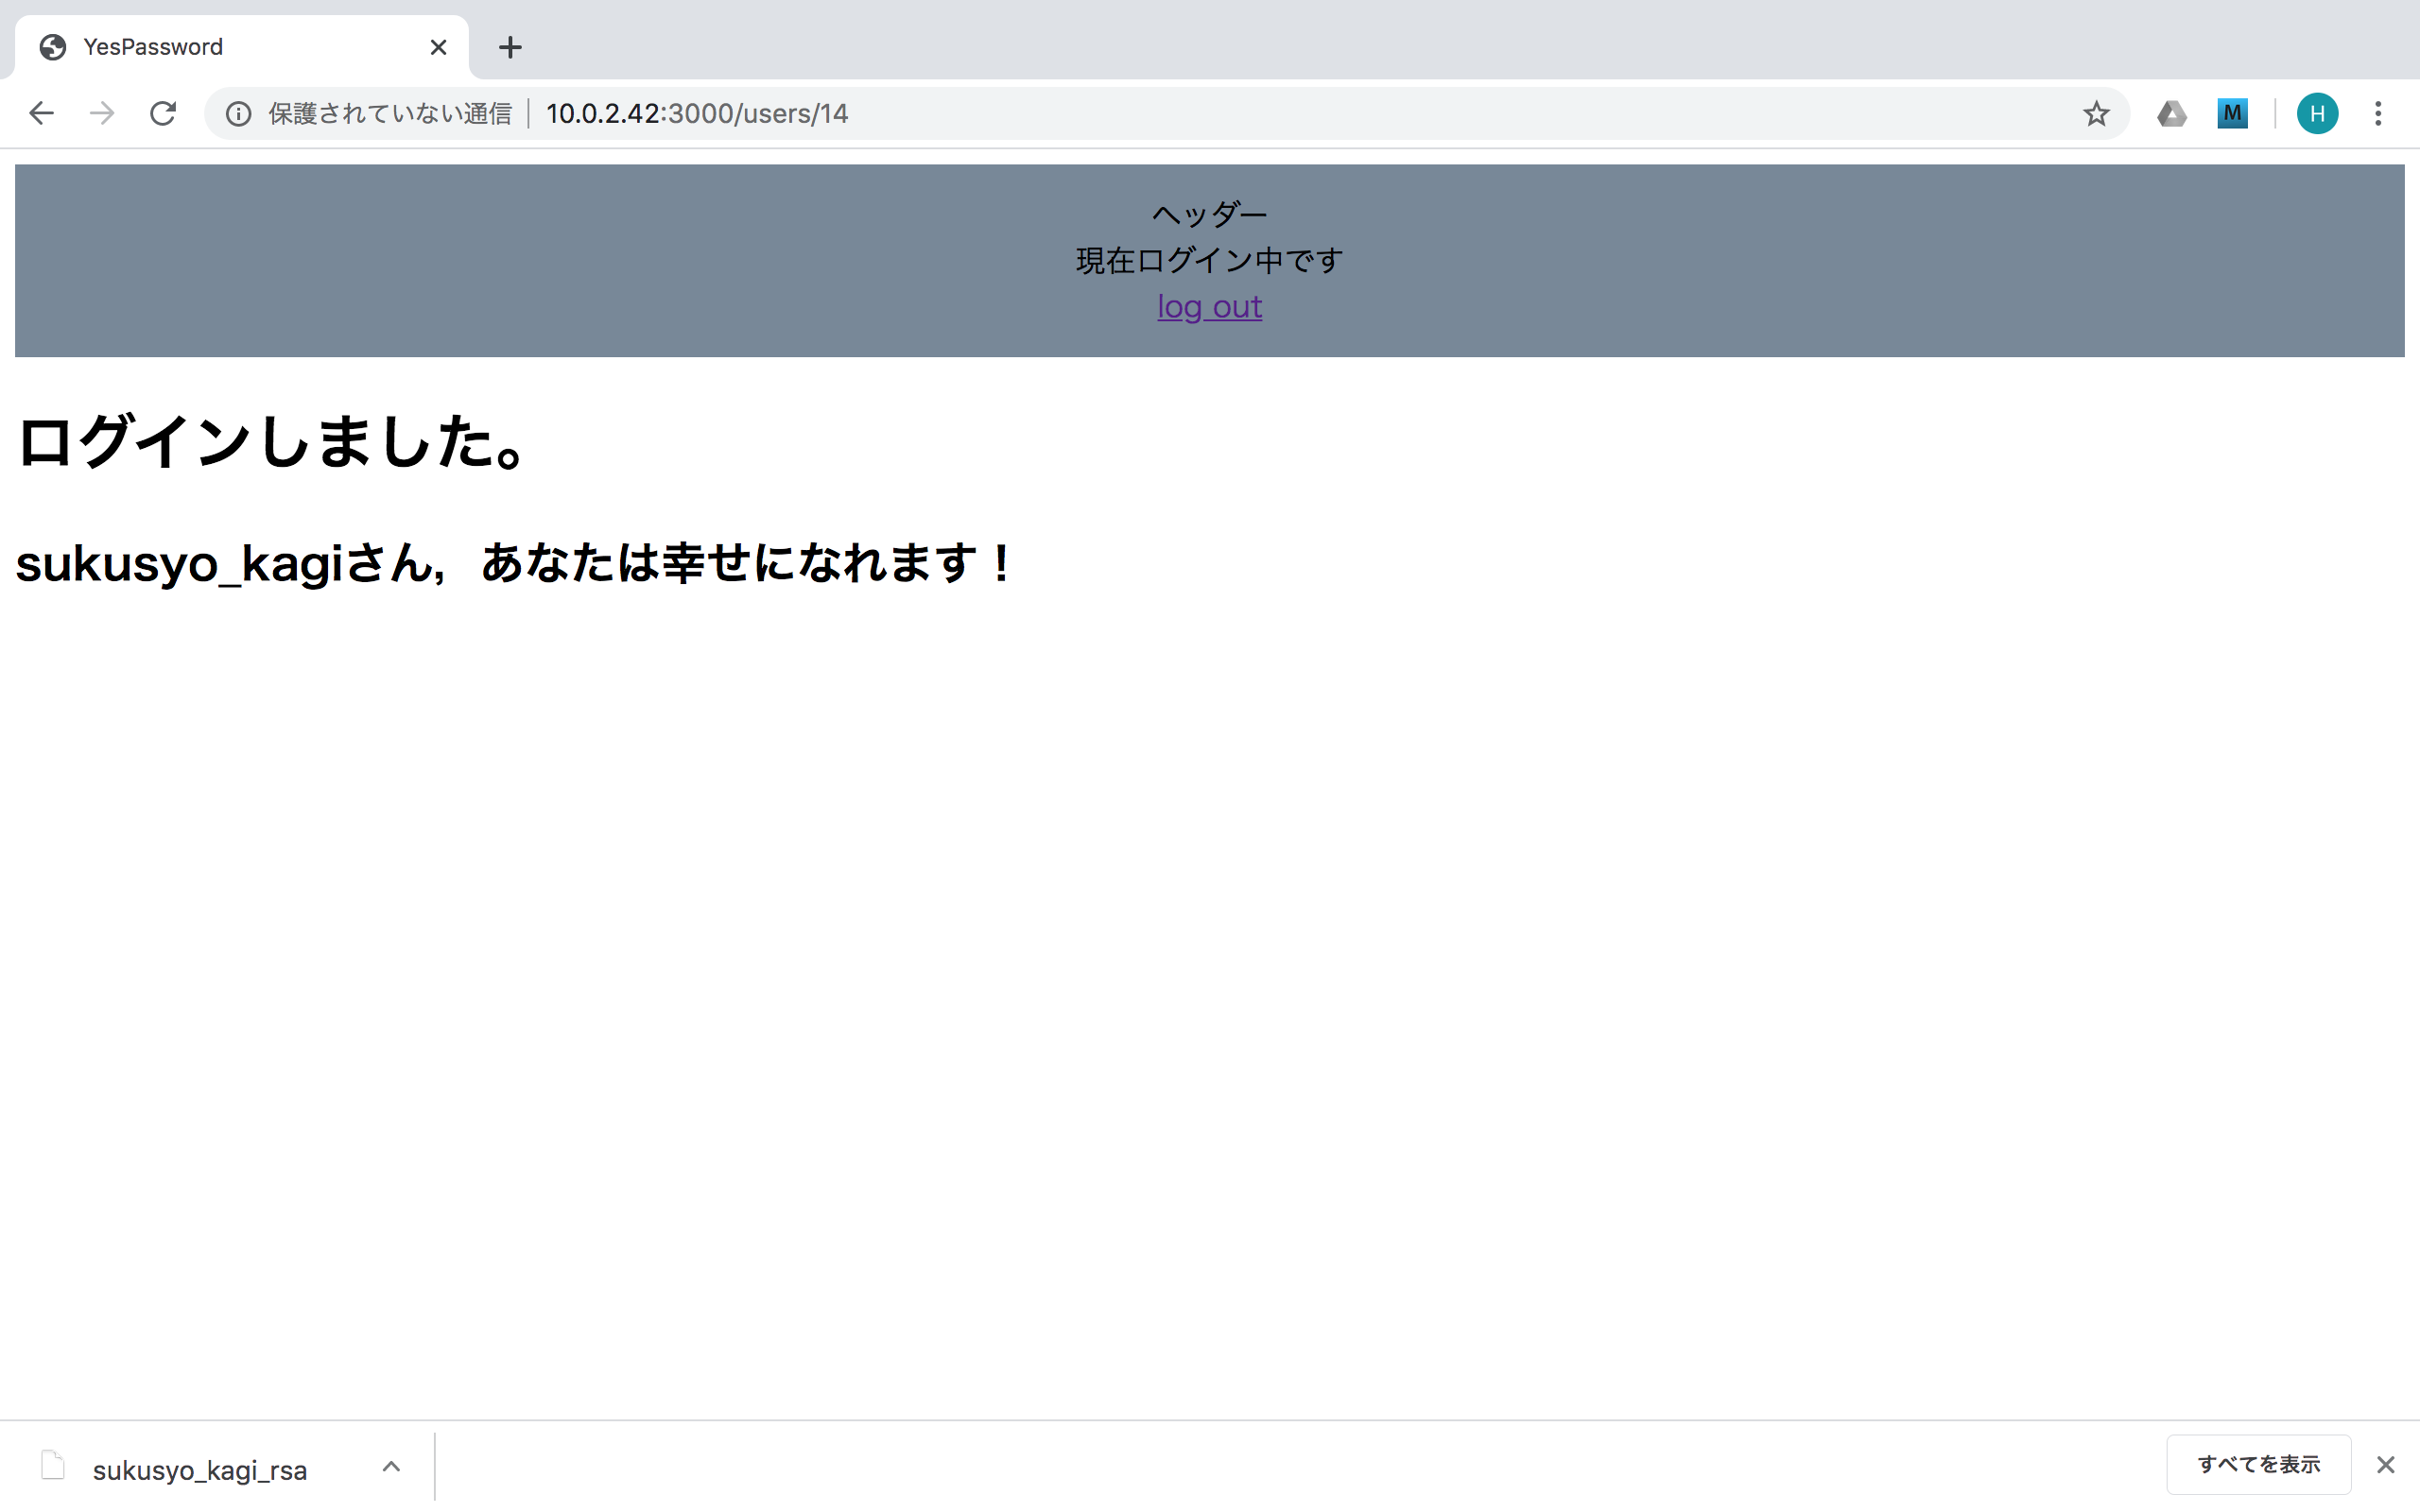
\includegraphics[height=8.4cm]{./fig/chapter4/inspect_2/key_screnn/login-after2.png}
        \caption{検証2\_認証成功後(鍵方式)}
        \label{検証2認証成功後(鍵方式)}
    \end{figure}
    % 鍵方式のスクショ---------------------------------- 

    % アンケートは検証1と同じ質問(意図)をしているため,割愛する。








   
    \newpage


    \subsubsection{検証マニュアル}
    以下の図\ref{検証2マニュアル1},図\ref{検証2マニュアル2},図\ref{検証2マニュアル3}は,上記の図\ref{検証2アカウント作成(パスワード方式)} 〜 図\ref{検証2アカウント作成(鍵方式)} ,図\ref{アンケート1} 〜 図\ref{アンケート4}
    の検証を行うためのマニュアルである.
    マニュアルを作成して,検証を行った意図としては,再現性を持って検証を行うためである.

    次に,検証1のマニュアルと比べての相違点とその意図を以下に述べる.\\
    パスワードの使い回し,password というパスワードなど,日常的に設定しないと思われるパスワードの設定が見受けられた。
    そのため,マニュアル(図\ref{検証2マニュアル1})に 「普段用いるように」,と被験者に注意を促す。
    また,パスワードの設定に関して,日常的に設定ような,より効果的な検証を行うためには,
    アカウントの登録で,パスワードに対して,バリデーション(パスワードの制限)をすることがあげられる。
    しかし,今回の検証では,あえてバリデーションをかけないことにする。
    理由は,
        鍵認証方式の,セキュリティは脆弱性が大きいのに対して,
        パスワード方式のだけセキュアにすると,検証比較として適していないと判断したためである。

    %何をやっているのかわからない
    鍵方式での,登録・認証に関して「何やっているかわからない」という意見があった。
    よって,マニュアル(図\ref{検証2マニュアル1},図\ref{検証2マニュアル2})に,「"パスワード方式です" "鍵方式です"」と軽く説明を加える。
    また,鍵方式の登録・認証に対しての,説明を詳しくすると,
    一般的に普及している,パスワード方式 による,被験者の慣れ を検証に含めることができないので,
    軽く「"パスワード方式です" "鍵方式です"」という説明を加えることにする。

    % 言いたいやつ----------------------------------------------------------------------------------------------
    %% マニュアル面(被験者生の動作や生の声から)----------------------------

    %%% より,日常的な検証結果を得るために(パスワード設定)
    %%%%パスワードの使い回し,password というパスワードなど,日常的に設定しないと思われるパスワードの設定が見受けられた。
    %%%%そのため,マニュアル(図????)に 「普段用いるように」,と被験者に注意を促す。
    %%%%また,パスワードの設定に関して,日常的に設定ような,より効果的な検証を行うためには,
    %%%%アカウントの登録で,パスワードに対して,バリデーション(パスワードの制限)をすることがあげられる。
    %%%%しかし,今回の検証では,あえてバリデーションをかけないことにする。
    %%%%理由は,
    %%%%    鍵認証方式の,セキュリティは脆弱性が大きいのに対して,
    %%%%    パスワード方式のだけセキュアにすると,検証比較として適していないと判断したためである。

    %%% 何をやっているのかわからない
    %%%% 鍵方式での,登録・認証に関して「何やっているかわからない」という意見があった。
    %%%% よって,マニュアル(図????)に,「"パスワード方式です" "鍵方式です"」と軽く説明を加える。
    %%%% 鍵方式の登録・認証に対しての,説明を詳しくすると,
    %%%%    一般的に普及している,パスワード方式 による,被験者の慣れ を検証に含めることができないので,
    %%%% 軽く「"パスワード方式です" "鍵方式です"」という説明を加える。
    %% マニュアル面(被験者生の動作や生の声から)----------------------------

    % 言いたいやつ----------------------------------------------------------------------------------------------


    \newpage
    \vspace{4cm}%図の位置を正しくする!
    \begin{figure}[H]
        %\centering
        \includegraphics[width=15cm]{./fig/chapter4/inspect_2/manual/manual_1.pdf}
        \caption{検証2マニュアル1}
        \label{検証2マニュアル1}
    \end{figure}

    \vspace{4cm}%図の位置を正しくする!
    \begin{figure}[H]
        %\centering
        \includegraphics[width=15cm]{./fig/chapter4/inspect_2/manual/manual_2.pdf}
        \caption{検証2マニュアル2}
        \label{検証2マニュアル2}
    \end{figure}

    \vspace{4cm}%図の位置を正しくする!
    \begin{figure}[H]
        %\centering
        \includegraphics[width=15cm]{./fig/chapter4/inspect_2/manual/manual_3.pdf}
        \caption{検証2マニュアル3}
        \label{検証2マニュアル3}
    \end{figure}



\subsection{検証結果}
    \subsubsection{被験者について}
    \begin{itemize}
        \item 琉球大学情報工学科の学生(4人)
        \item 琉球大学情報工学科の教員(1人)
        \item 琉球大学機械システム工学科の学生(1人)
    \end{itemize}
    %琉球大学情報工学科の学生(4人)\\
    %琉球大学情報工学科の学生(1人)\\
    %琉球大学機械システム工学科の学生(1人)\\

    \subsubsection{時間の観点からの面倒さ}
        ここでは被験者に行ってもらった,登録・認証にかかる時間を以下の表\ref{検証2 認証・登録の計測時間}に示す.
        表\ref{検証2 認証・登録の計測時間} は パスワード方式,鍵方式の登録・認証それぞれについて,個の時間,平均時間を記述した表である.
        被験者6に関しては,password方式の実装の2つの問題点により,計測ができなかったため,省く.
            % 2つの問題点について
                % バグ(登録できるが,認証ができない){同じメアドで登録できてしまうから}
                % パスワード確認入力欄が無い
            %+アルファー
                % 情報工学科以外の ゆういつ の被験者 -> パソコン操作に慣れていない
                %$ --> 今後の課題として,パソコン操作に慣れていない人でも,使いやすいようにする?????
        %表の記述
        \begin{table}[htb]
            \caption{検証2\_認証・登録の計測時間}
            \label{検証2 認証・登録の計測時間}
            \begin{tabular}{|l|r|r|r|r|r|r|r|} \hline%| (ハイプ) は縦線
                %登録・認証の種類 \textbackslash 被験者 & 被験者1 & 被験者2 & 被験者3  & 被験者4 & 平均\\ \hline%\hline は横の線
                                    & 被験者5 & 被験者7 & 被験者8 & 被験者9 & 被験者10 & 被験者11 & 平均 \\ \hline%\hline は横の線
                登録(パスワード方式) & 29.68 & 20.56   & 16.20 & 42.06   & 51.85   & 17.88   & 29.71\\ \hline
                認証(パスワード方式) & 17.29 & 14.95   & 10.40 & 17.95   & 19.62   & 13.33   & 15.59\\ \hline
                登録(鍵方式)        & 11.26 & 11.06   & 8.53  & 19.18   & 12.16   & 11.98   & 12.36\\ \hline
                認証(鍵方式)        & 13.63 & 16.23   & 8.65  & 43.83   & 12.3    & 15.51   & 18.36\\ \hline
    
                %----- 最終ページの表の最下部 --------
                \multicolumn{6}{r}{\small\it (単位:秒)}\\
            \end{tabular}
        \end{table}
    
        %上の表の参考方法
        %%表\ref{検証2 認証・登録の計測時間}


    \subsubsection{アンケートの観点からの面倒さ}
        ここでは,被験者に対して,2つの方式の登録・認証が終わった直後に,
        記入してもらったアンケートについての数値のまとめを以下の表\ref{検証1 アンケートによる6段階評価}に示す.
        表\ref{検証1 アンケートによる6段階評価}は 被験者による パスワード方式,鍵方式の登録・認証それぞれについて0 〜 5 段階評価,さらに,検証自体の面倒さについての評価を加えて まとめた表である.
        被験者6に関しては,password方式の実装の2つの問題点により,時間の計測ができなかったため,省く.
        %表の記述
        \begin{table}[htb]
            \caption{検証2\_アンケートによる6段階評価}
            \label{検証2 アンケートによる6段階評価}
            \begin{tabular}{|l|r|r|r|r|r|r|r|} \hline%| (ハイプ) は縦線
                %登録・認証の種類 \textbackslash 被験者 & 被験者1 & 被験者2 & 被験者3  & 被験者4 & 平均\\ \hline%\hline は横の線
                                          & 被験者5 & 被験者7 & 被験者8 & 被験者9 & 被験者10 & 被験者11 & 平均 \\ \hline%\hline は横の線
                % 改行するために
                \begin{tabular}{l}
                    登録(パスワード方式)\\の面倒さ
                \end{tabular}
                                          & 1 & 4 & 2 & 2 & 1 & 3 & 2.17 \\ \hline%6
                % 改行するために
                \begin{tabular}{l}
                    認証(パスワード方式)\\の面倒さ  
                \end{tabular}
                                         & 1 & 3 & 2 & 2 & 2 & 3 & 2.17  \\ \hline
                登録(鍵方式)の面倒さ        & 0 & 2 & 0 & 2 & 0 & 2 & 1.00  \\ \hline
                認証(鍵方式)の面倒さ        & 1 & 1 & 1 & 2 & 1 & 2 & 1.33  \\ \hline
                検証自体の面倒さ           & 0 & 2 & 0 & 3 & 0 & 0 & 0.83  \\ \hline
    
                %----- 最終ページの表の最下部 --------
                \multicolumn{6}{r}{\small\it (0 〜 5段階)}\\
            \end{tabular}
        \end{table}
        %上の表の参考方法
        %%表\ref{検証2 アンケートによる6段階評価}


  \newpage

  \subsection{考察}
  検証者6の検証は失敗した.鍵方式の登録の検証の際,認証まで進んでしまい,データの取得ができなかったためである.
  そのことから,次の考察ができる.
    被験者6は,唯一 情報工学科でない学生であった.他の情報工学科の被験者と比較して,
    PCを専門にしていない学生である.そのことから,より利用者目線の被験者だと言える.
    利用者目線では,今回の鍵方式は使いづらい認証方式になっていると考察することができる.

    被験者7の認証(表\ref{検証2 認証・登録の計測時間})に注目すると,パスワード方式に比べて鍵方式の方が時間がかかっている.
    しかし,アンケートによる認証の面倒さ(表\ref{検証2 アンケートによる6段階評価})に着目すると,鍵方式に比べてパスワード方式の方が面倒 という数値になっている.
    また,被験者7の検証後に次のことを聞いた.「また,検証後に次のことを聞いた.「(公開鍵暗号方式方式)わかっているから,簡単だった」」
    被験者6と比較すると,鍵認証方式について次のことが考察できる.
    公開鍵暗号方式の知識を持っている人は,公開鍵暗号方式の知識を持っていない人に比べて,簡単に感じる傾向があるということが考えられる.


% 今後の課題
\chapter{今後の課題}

この章では,鍵方式の実装・検証について,今後の課題を列挙し,説明をする.\\
以下に,今後の課題を列挙する.
\begin{itemize}
    \item セキュリティの脆弱性の改善
    \begin{itemize}
        \item http通信を行なっていることの改善
        \item 秘密鍵を通信していることの改善
        \item CSRFトークンOFF\cite{CSRF-token}した上での実装
    \end{itemize}
    \item 利用者視点で使いやすいようにする
        \begin{itemize} 
            \item 鍵を紛失した時の再発行をできるようにする
            \item 鍵の管理を行いやすいようにする
            \item 鍵方式を知らない人でも使えるようにようにする
    \end{itemize}
    \item 鍵方式の登録・認証がセキュアな上での検証を行う.

\end{itemize}



% 参考文献
% 参考文献
\def\line{−\hspace*{-.7zw}−}

\begin{thebibliography}{99}
%\bibitem{*}内の * は各自わかりやすい名前などをつけて、
%論文中には \cite{*} のように使用する。
%これをベースに書き換えた方が楽かも。
%書籍、論文、URLによって若干書き方が異なる。
%URLを載せる人は参考にした年月日を最後に記入すること。


%\bibitem{hoge}
%hoge
% 背景と目的のところ
\bibitem{first-safety1} マスタリングTCP/IP 入門編 第5版 , 2016 , オーム社 , 序文,p11
\bibitem{first-safety2} マスタリングTCP/IP 情報セキュリティ編 第1版 , 2014 , オーム社 , p18
\bibitem{first-password1} 7割以上のサービスが「IDとパスワードのみの認証」、多要素認証の採用に遅れ\\ https://www.is702.jp/news/3520/ \\最終閲覧日:2019/10/09
\bibitem{first-password2} 「8文字(8桁)のパスワード」は今では時代遅れでかなり危険。どうしたら安全? \\ https://keepmealive.jp/8letters-danger/ \\最終閲覧日:2019/10/17

% 技術概要のところ
\bibitem{technology-authentication} \url{https://www.fom.fujitsu.com/goods/pdf/security/fpt1610-2.pdf} \\最終閲覧日:2019/10/10
\bibitem{technology-authentication-2} マスタリングTCP/IP 情報セキュリティ編 第1版 , 2014 , オーム社 , p68 〜 p75 
\bibitem{technology-SSH_authentication} マスタリングTCP/IP 情報セキュリティ編 第1版 , 2014 , オーム社 , p34 



% 提案手法ボツ案? のところだったはず!
\bibitem{cookie1} \url{https://tools.ietf.org/html/rfc6265#section-1} \\ 最終閲覧日:2020/1/20
\bibitem{cookie2} \url{https://qiita.com/mogulla3/items/189c99c87a0fc827520e} \\ 最終閲覧日:2020/1/20
\bibitem{cookie-httponly-default} \url{https://qiita.com/yasu/items/8ae3077bdbee606681f6#cookiestore%E3%81%8C%E5%95%8F%E9%A1%8C%E3%81%AA%E3%81%AE%E3%81%8B} \\ 最終閲覧日:2020/1/21
\bibitem{cookie-httponly-security} \url{https://developer.mozilla.org/ja/docs/Web/HTTP/Cookies} \\最終閲覧日:2020/1/21



% 今後の課題のところ
\bibitem{CSRF-token} \url{https://qiita.com/nishina555/items/4ffaf5cc57a384b66230} \\ 最終閲覧日:2020/2/15

\end{thebibliography}




% 謝辞
\chapter*{謝辞}
\thispagestyle{empty}

%基本的な内容は以下の通り.参考にしてみて下さい.
%厳密な決まりは無いので,個々人の文体でも構わない.
%GISゼミや英語ゼミに参加した人はその分も入れておく.
%順番は重要なので気を付けるように.(提出前に周りの人に確認してもらう.)

\hspace{1zw}本研究の遂行,また本論文の作成にあたり、御多忙にも関わらず,主体的な学びが成長につながるという方針で,私の主体性を伸ばし,尊重してくれた長田智和助教授に深く感謝したします

研究の実装で,砂漠で道に迷っているような時に,方位磁石のように方針の提案をしてくれた秋田さん。研究の実装で,赤子が歩き方をわからないような状態の時に,歩き方を教えてくれた田場さん。深く考えさせるようなアドバイスをくれただいすけさん.インフラのことを教えてくれたり,論文の添削をしてくれた城後さん。開発で詰まった際に,アドバイスをくれた津嘉山さん。数々の貴重な御助言と細かな御配慮を戴き,深く感謝いたします.


また,一年間コミュ障な私に,気軽に接してくれた,ta-hi君,たかひろくん,棚原くん,喜納くんに感謝致します。

最後に、有意義な時間を共に過ごした情報工学科の学友、並びに物心両面で支えてくれた両親に深く感謝致します。

\begin{flushright}
 2020年 3月 \\ 与那嶺東
\end{flushright}




% 付録
%\input{appendix.tex}

\end{document}
